%%%%%%%%%%%%%%%%%%%%%%%%%%%%%%%%%%%%%%%%%
% Masters/Doctoral Thesis 
% LaTeX Template
% Version 2.5 (27/8/17)
%
% This template was downloaded from:
% http://www.LaTeXTemplates.com
%
% Version 2.x major modifications by:
% Vel (vel@latextemplates.com)
%
% This template is based on a template by:
% Steve Gunn (http://users.ecs.soton.ac.uk/srg/softwaretools/document/templates/)
% Sunil Patel (http://www.sunilpatel.co.uk/thesis-template/)
%
% Template license:
% CC BY-NC-SA 3.0 (http://creativecommons.org/licenses/by-nc-sa/3.0/)
%
%%%%%%%%%%%%%%%%%%%%%%%%%%%%%%%%%%%%%%%%%

%----------------------------------------------------------------------------------------
%	PACKAGES AND OTHER DOCUMENT CONFIGURATIONS
%----------------------------------------------------------------------------------------

\documentclass[
11pt, % The default document font size, options: 10pt, 11pt, 12pt
%oneside, % Two side (alternating margins) for binding by default, uncomment to switch to one side
ngerman,
english, % ngerman for German
singlespacing, % Single line spacing, alternatives: onehalfspacing or doublespacing
%draft, % Uncomment to enable draft mode (no pictures, no links, overfull hboxes indicated)
%nolistspacing, % If the document is onehalfspacing or doublespacing, uncomment this to set spacing in lists to single
%liststotoc, % Uncomment to add the list of figures/tables/etc to the table of contents
%toctotoc, % Uncomment to add the main table of contents to the table of contents
%parskip, % Uncomment to add space between paragraphs
%nohyperref, % Uncomment to not load the hyperref package
headsepline, % Uncomment to get a line under the header
%chapterinoneline, % Uncomment to place the chapter title next to the number on one line
%consistentlayout, % Uncomment to change the layout of the declaration, abstract and acknowledgements pages to match the default layout
]{MastersDoctoralThesis} % The class file specifying the document structure

%\usepackage[utf8x]{inputenc} 
\usepackage[utf8]{inputenc} % Required for inputting international characters

\usepackage[T1]{fontenc} % Output font encoding for international characters

\usepackage{mhchem} % chemical reactions 

%\usepackage{mathpazo} % Use the Palatino font by default
\usepackage{lmodern} % Use the Latin Modern font by default

%\usepackage[backend=bibtex,style=authoryear,natbib=true]{biblatex} % Use the bibtex backend with the authoryear citation style (which resembles APA)
\usepackage[backend=bibtex,style=numeric-comp,natbib=true,sorting=none]{biblatex} % Use the bibtex backend with the numeric-comp citation style (which resembles APA), sorting=none is for sorting reference automatically.
%\usepackage[square,numbers]{natbib}

\addbibresource{example.bib} % The filename of the bibliography

\usepackage[autostyle=true]{csquotes} % Required to generate language-dependent quotes in the bibliography
%====================
% To strike out sth
\usepackage{calc}
\newsavebox\CBox
\newcommand\hcancel[2][0.5pt]{%
  \ifmmode\sbox\CBox{$#2$}\else\sbox\CBox{#2}\fi%
  \makebox[0pt][l]{\usebox\CBox}%  
  \rule[0.5\ht\CBox-#1/2]{\wd\CBox}{#1}}
% Example: \hcancel[2pt]{xxx}
%====================
\usepackage[normalem]{ulem}
%\usepackage{amsmath} 
\newcommand{\stkout}[1]{\ifmmode\text{\sout{\ensuremath{#1}}}\else\sout{#1}\fi}
%====================

% add from other template
\usepackage{amsmath, amssymb}
%\usepackage{graphics} 
\usepackage{wrapfig,lipsum,booktabs}
\usepackage{setspace}
\usepackage{enumerate}
\usepackage[]{subfig}
%\usepackage{fancyhdr}
\usepackage{eucal}
\usepackage[below]{placeins}
%\usepackage[english]{babel}
%\usepackage[usenames, dvipsnames]{color}
%\usepackage[perpage]{footmisc}
%\usepackage{multirow}
%\usepackage{ifthen}
%\usepackage[square,sort,comma,numbers]{natbib} % Gang
\usepackage{mathrsfs} % Curlicue characters %Gang
%\usepackage{dcolumn}% Align table columns on decimal point %Gang
\usepackage{bm}% bold math %Gang
\usepackage{sidecap} %Gang
% Nomenclature
\usepackage{nomencl}
\usepackage{graphicx} % Include figure files
\usepackage{epstopdf} % PDFLATEX is not able to handle EPS graphic files, but converters epstopdf will help. The best way is to include epstopdf, which must follow the graphicx package
\usepackage{float}  %introduces a placement option H enforcing the placement exactly at that point.
\usepackage{placeins} %provides the command \FloatBarrier to limit the floating of figures or tables. You could place such a barrier before and after a listing.
\usepackage{xcolor}
\usepackage{color}
\usepackage{soul}
\usepackage{xspace} %In order to have space after "\newcommands" 
\usepackage{listings} %use for listing source codes
%\usepackage[all,cmtip]{xy}  %xypic
\lstset{ 
    language=python, % choose the language of the code
    basicstyle=\fontfamily{pcr}\selectfont\footnotesize\color{black},
    %keywordstyle=\color{red}\bfseries, % style for keywords
    keywordstyle=\color{black}\bfseries, % style for keywords % Gang
    numbers=none, % where to put the line-numbers
    numberstyle=\tiny, % the size of the fonts that are used for the line-numbers     
    backgroundcolor=\color{white}, % we can also choose: darkgray
    showspaces=false, % show spaces adding particular underscores
    showstringspaces=false, % underline spaces within strings
    showtabs=false, % show tabs within strings adding particular underscores
    frame=single, % adds a frame around the code
    tabsize=2, % sets default tabsize to 2 spaces
    rulesepcolor=\color{gray},
    rulecolor=\color{black},
    captionpos=b, % sets the caption-position to bottom
    breaklines=true, % sets automatic line breaking
    breakatwhitespace=false, 
}
%\usepackage[toc,page]{appendix} %For adding appendices
\usepackage{pgfplots} % a plotting package in latex
\usepackage[export]{adjustbox}[2011/08/13]

%=================================================
%(Re-)New commands
%=================================================
%\renewcommand{\nomname}{List of Symbols and Abbreviations}
\newcommand{\etal}{\textit{et al.}}
\newcommand{\abinitio}{\textit{ab initio}\xspace}
\newcommand{\Li}{Li$^{+}$\xspace}
\newcommand{\Na}{Na$^{+}$\xspace}
\newcommand{\K}{K$^{+}$\xspace}
\newcommand{\Cl}{Cl$^{-}$\xspace}
\newcommand{\Br}{Br$^{-}$\xspace}
\newcommand{\I}{I$^{-}$\xspace}
\newcommand{\li}{Li$^{+}$}
\newcommand{\na}{Na$^{+}$}
\newcommand{\pot}{K$^{+}$}
\newcommand{\cl}{Cl$^{-}$}
\newcommand{\br}{Br$^{-}$}
\newcommand{\Iodine}{I$^{-}$}
\newcommand{\COO}{COO$^{-}$\xspace}
\newcommand{\sfg}{Sum Frequency Generation\xspace}
%\newcommand{\cm}{cm$^{-1}$~\xspace}
\newcommand{\cm}{cm$^{-1}$\thinspace}
\newcommand{\centimeter}{cm$^{-1}$}
\newcommand{\nm}{nm$^{-2}$\xspace}
\newcommand{\z}{\textit{z}-axis\xspace}
\newcommand{\water}{H$_2$O\xspace}
\newcommand{\wat}{H$_2$O}
\newcommand{\NVT}{\textit{NVT}\xspace}
\newcommand{\T}{\textit{T}\xspace}
\newcommand{\nitrate}{NO$_3^-$\xspace}
\newcommand{\nit}{NO$_3^-$}
\newcommand{\LiN}{LiNO$_3$\xspace}
\newcommand{\X}{$x$\xspace}
\newcommand{\Y}{$y$\xspace}
\newcommand{\Z}{$z$\xspace}
\newcommand*{\tran}{^{\mkern-1.5mu\mathsf{T}}}

%
\newcommand{\rt}{$t_\text{t}$\xspace}

%
\newcommand{\hbo}{$h(t)$\xspace}
\newcommand{\hbos}{$h^\text{(s)}(t)$\xspace}
\newcommand{\CHB}{$c(t)$\xspace}
\newcommand{\SHB}{$s(t)$\xspace}
\newcommand{\CSHB}{$c^\text{(s)}(t)$\xspace}
\newcommand{\SSHB}{$s^\text{(s)}(t)$\xspace}
\newcommand{\LiFourW}{[Li$\cdot$(H$_2$O)$_4$]$^+$}
\newcommand{\rI}{$r_{\text{I}^-}$}
\newcommand{\rcation}{$r_\text{cation}$}
%Renew the \AA command in order to have a space when we want
\let\oldAA\AA
\renewcommand{\AA}{\oldAA\xspace}
\newcommand{\A}{\oldAA}
%=================================================

%----------------------------------------------------------------------------------------
%	MARGIN SETTINGS
%----------------------------------------------------------------------------------------

\geometry{
	paper=a4paper, % Change to letterpaper for US letter
	inner=2.5cm, % Inner margin
	outer=3.8cm, % Outer margin
	bindingoffset=.5cm, % Binding offset
	top=1.5cm, % Top margin
	bottom=1.5cm, % Bottom margin
	%showframe, % Uncomment to show how the type block is set on the page
}

%----------------------------------------------------------------------------------------
%	THESIS INFORMATION
%----------------------------------------------------------------------------------------

\thesistitle{Structure, Dynamics and Vibrational Spectroscopy of Interfacial 
Alkali Nitrate and Alkali Halide Aqueous Solutions from \abinitio Molecular Dynamics} % Your thesis title, this is used in the title and abstract, print it elsewhere with \ttitle
\thesistitleG{Struktur-, Dynamik- und Schwingungsspektroskopie von Alkaligrenzflächen
Wässrige Nitratlösungen von \abinitio Molecular Dynamics} % Your thesis title, this is used in the title and abstract, print it elsewhere with \ttitle
\supervisor{Apl. Prof. Dr. Marialore \textsc{Sulpizi}} % Your supervisor's name, this is used in the title page, print it elsewhere with \supname
\examiner{Prof. Dr. Hartmut \textsc{Wittig}, Prof. Dr. Thomas \textsc{Palberg}, Prof. Dr. Hubert \textsc{Spiesberger}} % Your examiner's name, this is not currently used anywhere in the template, print it elsewhere with \examname
%\examiner{Prof. Dr. Hartmut \textsc{Wittig}} % Your examiner's name, this is not currently used anywhere in the template, print it elsewhere with \examname
\degree{Doctor of Philosophy} % Your degree name, this is used in the title page and abstract, print it elsewhere with \degreename
\degreeG{Doktor der Philosophie} % Your degree name, this is used in the title page and abstract, print it elsewhere with \degreename
\author{Gang \textsc{Huang}} % Your name, this is used in the title page and abstract, print it elsewhere with \authorname
\addresses{} % Your address, this is not currently used anywhere in the template, print it elsewhere with \addressname

\subject{Statistical Physics and Soft Matter} % Your subject area, this is not currently used anywhere in the template, print it elsewhere with \subjectname
\subjectG{Statistische Physik und weiche Materie} % Your subject area, this is not currently used anywhere in the template, print it elsewhere with \subjectname
\keywords{sum-frequency generation, hydrogen bond dynamics, water/vapor interfaces} % Keywords for your thesis, this is not currently used anywhere in the template, print it elsewhere with \keywordnames
\keywordsG{Summenfrequenzerzeugung, Wasserstoffbrückendynamik, Wasser/Dampf-Grenzflächen} % Keywords for your thesis, this is not currently used anywhere in the template, print it elsewhere with \keywordnames
\university{\href{https://www.uni-mainz.de}{Johannes Gutenberg University Mainz}} % Your university's name and URL, this is used in the title page and abstract, print it elsewhere with \univname
\universityG{\href{https://www.uni-mainz.de}{Johannes Gutenberg Universit\"at Mainz}} % Your university's name and URL, this is used in the title page and abstract, print it elsewhere with \univname
\department{\href{https://www.iph.uni-mainz.de}{Institute for Physics }} % Your department's name and URL, this is used in the title page and abstract, print it elsewhere with \deptname
\departmentG{\href{https://www.iph.uni-mainz.de}{Institut für Physik}} % Your department's name and URL, this is used in the title page and abstract, print it elsewhere with \deptname
\group{\href{https://www.komet1.physik.uni-mainz.de}{Condensed Matter Theory Group}} % Your research group's name and URL, this is used in the title page, print it elsewhere with \groupname
\groupG{\href{https://www.komet1.physik.uni-mainz.de}{Gruppe zur Theorie der kondensierten Materie}} % Your research group's name and URL, this is used in the title page, print it elsewhere with \groupname
\faculty{\href{https://www.komet1.physik.uni-mainz.de}{Condensed Matter Theory}} % Your faculty's name and URL, this is used in the title page and abstract, print it elsewhere with \facname
\facultyG{\href{https://www.komet1.physik.uni-mainz.de}{Theorie der kondensierten Materie}} % Your faculty's name and URL, this is used in the title page and abstract, print it elsewhere with \facname

\AtBeginDocument{
\hypersetup{pdftitle=\ttitle} % Set the PDF's title to your title
\hypersetup{pdfauthor=\authorname} % Set the PDF's author to your name
\hypersetup{pdfkeywords=\keywordnames} % Set the PDF's keywords to your keywords
}

\DeclareUnicodeCharacter{2212}{-} % Minus sign (by Gang Huang)


\begin{document}

\frontmatter % Use roman page numbering style (i, ii, iii, iv...) for the pre-content pages

\pagestyle{plain} % Default to the plain heading style until the thesis style is called for the body content

%----------------------------------------------------------------------------------------
%	TITLE PAGE
%----------------------------------------------------------------------------------------

\begin{titlepage}
\begin{center}

\vspace*{.06\textheight}
{\scshape\LARGE \univname\par}\vspace{1.5cm} % University name
\textsc{\Large Doctoral Thesis}\\[0.5cm] % Thesis type

\HRule \\[0.4cm] % Horizontal line
{\huge \bfseries \ttitle\par}\vspace{0.4cm} % Thesis title
\HRule \\[1.5cm] % Horizontal line
 
\begin{minipage}[t]{0.4\textwidth}
\begin{flushleft} \large
\emph{Author:}\\
\href{https://hg08.github.io}{\authorname} % Author name - remove the \href bracket to remove the link
\end{flushleft}
\end{minipage}
\begin{minipage}[t]{0.5\textwidth}
\begin{flushright} \large
\emph{Supervisor:} \\
\href{https://www.staff.uni-mainz.de/sulpizi}{\supname} % Supervisor name - remove the \href bracket to remove the link  
%\end{flushright}
%\end{minipage}\\[1cm]
%\begin{minipage}[t]{0.5\textwidth}
%\begin{flushleft} \large
\emph{Second reviewer:}\\
%Eximiners' name - remove the \href bracket to remove the link
\href{https://sites.google.com/site/jamirmarino/home}{J-Prof. Dr. Jamir \textsc{Marino}}\\
\end{flushright}
\end{minipage}\\[3cm]
 
\vfill

	\large \textit{A thesis submitted for the award of the title "Doctor of Natural Sciences"} \\[0.3cm] % University requirement text
\textit{to the Faculty of}\\[0.4cm]
	Physics, Mathematics and Computer Science of \\
	{\univname\par} %Johannes Gutenberg University Mainz in Mainz
%\groupname\\\deptname\\[2cm] % Research group name and department name
 
\vfill

{\large 2021}\\[4cm] % Date
%\includegraphics{Logo} % University/department logo - uncomment to place it
 
\vfill
\end{center}
\end{titlepage}

%----------------------------------------------------------------------------------------
%	DECLARATION PAGE
%----------------------------------------------------------------------------------------

\begin{declaration}
\addchaptertocentry{\authorshipname} % Add the declaration to the table of contents
\noindent I, \authorname, declare that this thesis titled, \enquote{\ttitle} and the work presented in it are my own. I confirm that:

\begin{itemize} 
\item This work was done wholly or mainly while in candidature for a research degree at this University.
\item Where any part of this thesis has previously been submitted for a degree or any other qualification at this University or any other institution, this has been clearly stated.
\item Where I have consulted the published work of others, this is always clearly attributed.
\item Where I have quoted from the work of others, the source is always given. With the exception of such quotations, this thesis is entirely my own work.
\item I have acknowledged all main sources of help.
\item Where the thesis is based on work done by myself jointly with others, I have made clear exactly what was done by others and what I have contributed myself.\\
\end{itemize}
 
\noindent Signed:\\
\rule[0.5em]{25em}{0.5pt} % This prints a line for the signature
 
\noindent Date:\\
\rule[0.5em]{25em}{0.5pt} % This prints a line to write the date
\end{declaration}

\cleardoublepage

%----------------------------------------------------------------------------------------
%	QUOTATION PAGE
%----------------------------------------------------------------------------------------

\vspace*{0.2\textheight}

%\noindent\enquote{\itshape The accurate description of water has been and continues to be a challenge for both
%experiment and simulations due to the directional nature and the weakness of the hydrogen bonds in conjunction 
%with its autodissociation properties.}\bigbreak

%\hfill Dominik Marx  and J\"urg Hutter 

\noindent\enquote{\itshape If a problem is worth looking at at all, then no mathematical technique is to be judged too sophisticated.}\bigbreak

\hfill David Ruelle 

%----------------------------------------------------------------------------------------
%	ABSTRACT PAGE
%----------------------------------------------------------------------------------------

\begin{abstract}
\addchaptertocentry{\abstractname} % Add the abstract to the table of contents
The interfacial structure and dynamics of solutions containing alkali nitrates and alkali halides have been studied by density functional theory-based 
molecular dynamics (DFTMD) simulations. We have presented a detailed analysis of the hydrogen bond (HB) structure at the interface and 
calculated the interface vibrational sum-frequency generation (VSFG) spectra to provide a molecular interpretation of the available experimental data.

Both the measured and the calculated VSFG spectra of the alkali nitrate solution show a reduced intensity 
in the lower frequency portion of the stretching band, compared with the water/vapor interface.
This reduction is attributed to the hydrogen (H-) bonds established between nitrate and the surrounding water molecules at the interface.
This spectral feature is only related to the presence of nitrate at the water surface and is not influenced by the alkali metal ions.
We have also shown that, to provide a microscopic interpretation of the spectra,
realistic models of the interface are required beyond simple cluster models.

Heavier halide anions such as iodine have an effect similar to that of nitrate on the structure and dynamics of the water/vapor interface.
From the results of the simulations and the calculation of the nonlinear susceptibilities, 
we conclude that water molecules at the interfaces of LiI, NaI, and KI solutions are participating
in weaker H-bonds, compared with those at the water/vapor interface.
This feature originates from the unique distribution of \I ions and alkali metal cations,
which form a double layer over a thickness of about 5--10 \A.

The second aspect we have investigated is the HB dynamics.
To analyze HB dynamics at interfaces, 
we determined the instantaneous interface based on spatial density, 
and proposed a statistical scheme based on the interfacial HB (IHB) population for identifying the instantaneous interface.
Combining the IHB method with interfacial molecule sampling (IMS), we obtained a method to determine the thickness of the water/vapor interface.
The IHB method has also been extended to the solvation shells of ions in aqueous solutions.

%Finally, the number $n$ of H-bonds per OH group at instantaneous interface promotes our understanding of structural features of the alkali nitrate
%	solution/vapor interface. 
%	By comparing the distribution $P(n)$ of $n$ between the \LiN solution/vapor interface and the water/vapor interface, 
%	we obtained that: For the solution interface, there is less free OH groups, and more OH groups that can form two H-bonds. 
%	This distribution verified the "water-separated cation-nitrate ion pair" structure; 
%	When the interface thickness is greater than 4 \A, the macroscopic properties of the solution interface, 
%	whether it is the distribution $P(n)$ or the relaxation time of the reorientation relaxation process, converge to the same as that of bulk water.
%	In addition, we have verified that the alkali iodide solutions also have these two properties.
\end{abstract}

%----------------------------------------------------------------------------------------
%	ABSTRACT PAGE GERMAN
%----------------------------------------------------------------------------------------
{\selectlanguage{ngerman}
\begin{extraAbstract}
\addchaptertocentry{\abstractname} % Add the abstract to the table of contents
Die Grenzflächenstruktur und -dynamik von Lösungen, die Alkalinitrate und Alkalihalogenide enthalten, 
wurden mit Hilfe von auf Dichtefunktionaltheorie basierenden Molekulardynamik-Simulationen (DFTMD) untersucht.
Wir haben eine detaillierte Analyse der Wasserstoffbrückenbindungsstruktur (HB) an der Grenzfläche durchgeführt und
berechneten die Spektren der Schwingungssummen-Frequenz-Generierung (VSFG) an der Grenzfläche, um eine molekulare Interpretation der verfügbaren experimentellen Daten zu ermöglichen.

Sowohl die gemessenen als auch die berechneten VSFG-Spektren der Alkalinitratlösung zeigen eine verminderte Intensität
im unteren Frequenzbereich der Streckbande im Vergleich zur Wasser-Dampf-Grenzfläche.
Diese Verringerung wird auf die Wasserstoffbrückenbindungen zurückgeführt, die zwischen Nitrat und den umgebenden Wassermolekülen an der Grenzfläche entstehen.
Dieses spektrale Merkmal hängt nur mit dem Vorhandensein von Nitrat an der Wasseroberfläche zusammen und wird nicht von den Alkalimetallionen beeinflusst.
Wir haben auch gezeigt, dass für eine mikroskopische Interpretation der Spektren
realistische Modelle der Grenzfläche erforderlich sind, die über einfache Clustermodelle hinausgehen.

Schwerere Halogenidanionen wie Jod haben einen ähnlichen Effekt wie Nitrat auf die Struktur und Dynamik der Wasser-Dampf-Grenzfläche.
Aus den Ergebnissen der Simulationen und der Berechnung der nichtlinearen Suszeptibilitäten,
schließen wir, dass die Wassermoleküle an den Grenzflächen von LiI-, NaI- und KI-Lösungen
an schwächeren H-Bindungen beteiligt sind als an der Wasser/Dampf-Grenzfläche.
Dieses Merkmal ist auf die einzigartige Verteilung von \I-Ionen und Alkalimetallkationen zurückzuführen,
die eine Doppelschicht über eine Dicke von etwa 5-10 \A\  bilden.

Der zweite Aspekt, den wir untersucht haben, ist die HB-Dynamik.
Um die HB-Dynamik an Grenzflächen zu analysieren,
haben wir die momentane Grenzfläche anhand der räumlichen Dichte bestimmt,
und schlugen ein statistisches Schema vor, das auf der HB-Population an den Grenzflächen (IHB) basiert, um die momentane Grenzfläche zu identifizieren.
Durch die Kombination der IHB-Methode mit dem Interfacial Molecule Sampling (IMS) erhielten wir eine Methode zur Bestimmung der Dicke der Wasser/Dampf-Grenzfläche.
Die IHB-Methode wurde auch auf die Solvatationsschalen von Ionen in wässrigen Lösungen ausgedehnt.

\end{extraAbstract}
}
\selectlanguage{english}
%----------------------------------------------------------------------------------------
%	ACKNOWLEDGEMENTS
%----------------------------------------------------------------------------------------

\begin{acknowledgements}
\addchaptertocentry{\acknowledgementname} % Add the acknowledgements to the table of contents
I wish to express my sincere gratitude to my supervisor,
Prof. Dr. Marialore Sulpizi for her excellent guidance during my doctoral studies, and her detailed and valuable advice for my writing.
I thank her for bringing me into interesting and novel areas of density functional theory-based molecular dynamics simulation 
and interface physics and chemistry. By communicating with her, I was implicitly and positively affected. 
She is rigorous in academic studies, optimistic and active, and has a wide range of interests. 
All these have kept in my heart and gave me greater confidence in my future work.

%
I am grateful to Prof. Dr. Friederike Schmid  and Prof. Dr. Kurt Binder for their talks and guidance.
I wish to thank Prof. Dr. Thomas Kühne, Dr. Giovanni Settanni, PD Dr. Peter
Virnau, Dr. Hans Behringer and Prof. Dr. Thomas Speck at the institute for
physics for leading me to the fundamental statistical physics and excellent lectures and discussions. 

%
I thank Prof. Dr. Harvey Meyer at the institute for nuclear physics. 
I feel very honored to be a teaching assistant in his quantum field theory course. 
%
I thank Prof. Marie-Pierre Gaigeot at Universit{\'e} d'Evry val d'Essonne for useful discussions.

%
I am grateful to Dr. R\'emi Khatib for helpful guidance on the programs for calculating the VSFG spectra. 
I thank Dr. Qi Shuanhu, Dr. Zhou Jiajia and Dr.Yu Fei for useful discussions. 
I would like to thank Leila Salimi, Isidro Lorenzo Geada, Santosh Kumar Meena and Anusha Lalitha, 
at the Institute for Physics, for their assistance.
%
I thank Astrid Chase, Andreas Nussbaumer and Daniela Reibel for their enthusiastic and patient help.

%
The financial supports of the China Scholarship Council and TRR146 are gratefully acknowledged.

%
I thank Prof. Luo Honggang, Prof. Fang Haiping and Prof. Zhou Haijun for their great help in my study during my doctoral studies. 
The cooperation and discussions with Dr. Shi Guosheng, Dr. Shao Junming, Dr. Zhou Bo and Dr. Wang Chunlei have benefited me a lot. 

%
I thank Prof. Jin Yuliang for his support, trust and teachings over the past two years.

%
I would like to thank the following teachers who have benefited me for life:
Mr. Lu Yongliang, Mr. Li Yiyou, 
Mr. Yang Bing, Mr. Chen Jiexian, Mr. Chen Jiangen, Mr. Li Yiji,
Mr. Wu Xiukui, Mr. Chen Wenfeng, Mr. Liao Changchun, Mr. Zhou Wende,
Mr. Yan Zhengzhou, Prof. Huang Ruibin, Prof. Ran Qiyin, Prof. Huang Yong, Prof. Luo Zhiquan, Prof. Fan Silin, Prof. Tao Caide, Prof. Ren Weiyi, 
Prof. Tan Lei and Prof. Liu Yuxiao.

%
I am grateful to my parents Diao Yuhua and Huang Dehuai, and my brother Jialiang, for their care, 
understanding and support for me for decades. 
This thesis is dedicated to my grandparents Zhong Yuhtsing, Diao Sherngwern, Ma Suhfang, and Huang Zongyirn. 
I will always remember the kindness, open-mindedness, diligence and perseverance.
\end{acknowledgements}

%----------------------------------------------------------------------------------------
%	LIST OF CONTENTS/FIGURES/TABLES PAGES
%----------------------------------------------------------------------------------------
{
\hypersetup{linkcolor=black}
\tableofcontents % Prints the main table of contents
}

{
\hypersetup{linkcolor=black}
\listoffigures % Prints the list of figures
}

{
\hypersetup{linkcolor=black}
\listoftables % Prints the list of tables
}

%----------------------------------------------------------------------------------------
%	ABBREVIATIONS
%----------------------------------------------------------------------------------------

\begin{abbreviations}{ll} % Include a list of abbreviations (a table of two columns)

\textbf{2DSFG} & two-\textbf{D}imensional \textbf{S}um-\textbf{F}requency \textbf{G}eneration\\
\textbf{AIMD} & \abinitio \textbf{M}olecular \textbf{D}ynamics\\
\textbf{BLYP} & \textbf{B}eck-\textbf{L}ee-\textbf{Y}ang-\textbf{P}arr\\
\textbf{BOMD} & \textbf{B}orn-\textbf{O}ppenheimer \textbf{M}olecular \textbf{D}ynamics\\
\textbf{CPMD} & \textbf{C}ar-\textbf{P}arrinello \textbf{M}olecular \textbf{D}ynamics\\
\textbf{DFT} & \textbf{D}ensity \textbf{F}unctional \textbf{T}heory\\
\textbf{DFTMD} & \textbf{D}ensity \textbf{F}unctional \textbf{T}heory-based \textbf{M}olecular \textbf{D}ynamics\\
\textbf{EDA} & \textbf{E}lectric \textbf{D}ipole \textbf{A}pproximation\\
\textbf{GGA} & \textbf{G}eneralised \textbf{G}radient \textbf{A}pproximation\\
\textbf{GPW} & \textbf{G}aussian and \textbf{P}lane \textbf{W}aves\\
\textbf{H-} & \textbf{H}ydrogen\\
\textbf{HB} & \textbf{H}ydrogen \textbf{B}ond\\
\textbf{HD} & \textbf{H}eterodyne \textbf{D}etected\\
\textbf{HK} & \textbf{H}ohenberg-\textbf{K}ohn\\
\textbf{IHB} & \textbf{I}nterfacial \textbf{H}ydrogen \textbf{B}ond\\
\textbf{IMS} & \textbf{I}nterfacial \textbf{M}olecule \textbf{S}ampling\\
\textbf{KS} & \textbf{K}ohn-\textbf{S}ham\\
\textbf{LDA} & \textbf{L}ocal \textbf{D}ensity \textbf{A}pproximation\\
\textbf{MD} & \textbf{M}olecular \textbf{D}ynamics\\
\textbf{MLWF} & \textbf{M}aximally-\textbf{L}ocalized \textbf{W}annier \textbf{F}unctions\\
\textbf{MP2} & \textbf{M}oller-\textbf{P}lesset \textbf{P}erturbation\\
\textbf{PBE} & \textbf{P}erdew-\textbf{B}urke-\textbf{E}rnzherhof\\
\textbf{PS} & \textbf{P}hase-\textbf{S}ensitive\\
\textbf{RDF} & \textbf{R}adial \textbf{D}istribution \textbf{F}unction\\
\textbf{SHB} & \textbf{S}olvation shell \textbf{H}ydrogen \textbf{B}ond\\
\textbf{SCF} & \textbf{S}elf \textbf{C}onsistent \textbf{F}ield\\
\textbf{VACF} & \textbf{V}elocity \textbf{A}uto-\textbf{C}orrelation \textbf{F}unction\\
\textbf{VDOS} & \textbf{V}ibrational \textbf{D}ensity \textbf{O}f \textbf{S}tates\\
\textbf{VSFG} & \textbf{V}ibrational \textbf{S}um-\textbf{F}requency \textbf{G}eneration\\
\textbf{XC} & e\textbf{X}change  and \textbf{C}orrelation\\

\end{abbreviations}

%----------------------------------------------------------------------------------------
%	PHYSICAL CONSTANTS/OTHER DEFINITIONS
%----------------------------------------------------------------------------------------

\begin{constants}{lr@{${}={}$}l} % The list of physical constants is a three column table

% The \SI{}{} command is provided by the siunitx package, see its documentation for instructions on how to use it

Avogadro constant & $N_{\text{A}}$ & 6.022 140 76 $\times 10^{23}$ /mol (exact) \\
%Constant Name & $Symbol$ & $Constant Value$ with units\\
Boltzmann constant & $k_{\text{B}}$ & 1.380 649 $\times 10^{23}$ \si{\joule\per\kelvin} (exact) \\
elementary charge & $e$  & 1.602 176 634 $\times 10^{-19}$ C (exact)\\
electron mass & $m_{\text{e}}$ & 9.109 381 887 $\times 10^{-31}$ kg \\
molar gas constant & $R$ & 8.314 459 8 J mol$^{-1}$ K$^{-1}$,\\
proton mass & $m_{\text{p}}$ & 1.672 621 581 $\times 10^{-27}$ kg \\
Planck constant & $h$ & 6.626 070 15 $\times 10^{-34}$ J s (exact) \\
reduced Planck constant & $\hbar$ & 1.054 571 817 $\times 10^{-34}$ J s\\
speed of light in vacuum  & $c$ & \SI{299 792 458}{\meter\per\second} (exact)
\end{constants}

%----------------------------------------------------------------------------------------
%	SYMBOLS
%----------------------------------------------------------------------------------------

\begin{symbols}{lll} % Include a list of Symbols (a three column table)

% $a$ & distance & \si{\meter} \\
% $P$ & power & \si{\watt} (\si{\joule\per\second}) \\
% $\omega$ & angular frequency & \si{\radian} \\
%Symbol & Name & Unit \\

\addlinespace % Gap to separate the Roman symbols from the Greek

%$f_i$ & activity coefficient of species $i$ & \\
$Z_{\text{X}}$ & atomic number of atom X & \\
${\bf R}$ & atomic coordinates & \\
$\tau_{\mathrm{a}}$ & average lifetime of H-bonds: $\langle\tau_{\mathrm{a}}\rangle = \int_0^\infty tP_{\mathrm{a}}(t) d t $ & \\
$\mu_i$ &chemical potential of component $i$ & \\
$\kappa_i$ & decay rate of $C_2(t)$ & \\
$n_{\text{X}}$ & coordination number for ion X & \\
$\delta_1$ & difference between the first peaks' positions of the RDFs $g_{X-O}$ and $g_{X-H}$ & \\
${\bf M}$ & dipole moment & \\
$\mu^{i,l,\epsilon}$ & dipole moment of the bond $\epsilon$ of the $i$-th water molecule in the lab frame & \\
$A$ & dipole polarizability (tensor) & \\
$D$ & direction cosine matrix  & \\
$r$ & distance & \\
${\mu}$ & electric dipole vector & \\
${\phi}$ & electric potential & \\
${\bf E}$ & electric field strength &  \\
$n({\bf r})$ & electron density & \\
$H_\text{e}$ & electronic many-body Hamiltonian & \\
$E_\text{I}({\bf R})$ & energy of the nuclei & \\
$V({\bf r})$ & external potential & \\
$V_{\text{ee}}$ & electron-electron repulsion energy & \\
$T[n]$ & electronic kinetic energy & \\
$E_{\text{disp}}^{(2)}$ & empirical two-body dispersion correction of energy & \\
$E_{\text{disp}}^{(3)}$ & empirical three-body nonadditivity dispersion correction of energy & \\
$E^{\text{XC}}[n]$ & Exchange correlation energy functional & \\
$\Delta F_{AB}$ & free energy difference between configuration A and B &  \\
$F_A$ & free energy of configuration A &  \\
$L_{\eta\kappa}$ & Fresnel coefficients & \\
$\omega_{\text{SFG}}$ & frequency of the sum-frequency generation beam & \\
$\omega_{\text{vis}}$ & frequency of the incident visible beam &  \\
$\omega_{\text{IR}}$ & frequency of the incident infrared beam &  \\
$V_{\text{H}}$ & Hartree potential of electrons & \\
$h(t)$ & HB population operator & \\
$h^{(d)}(t)$ & HB population operator (it is 1 if the tagged pair are closer than $r_{\text{OO}}^{\text{c}}$)& \\
$H(t)$ & HB population operator (continuously)& \\
$c(t)$ & HB population auto-correlation function & \\
$\omega_{\text{I}}$ & highest nuclear phonon frequency & \\
$\theta$ & H-O-H angle in a water molecule, or polar angle of a molecule&  \\
$\beta$ & hyperpolarizability, or reciprocal temperature & \\
$h^{(s)}(t)$ & interfacial HB population operator & \\
$j(t)$ & integrated flux departing the HB configuration space at time t & \\
$I_{\text{SFG}}$ & intensity of the sum-frequency generation beam & \\
$I_{\text{vis}}$ & intensity of the incident visible beam & \\
$I_{\text{IR}}$ & intensity of the incident infrared beam & \\
$r_{\text{OO}}$ & interoxygen distance & \\
${\delta}t$ & inverse sampling frequency & \\
$E^{\text{KS}}[n]$ & Kohn-Sham energy functional & \\
$\omega_{\text{e}}$ & the lowest electronic frequency &  \\
$r_{\text{OO}}^{\text{c}}$ & the maximum value of the interoxygen distance (in the definition of HB) & \\
$\phi^{\text{c}}$ & the maximum value of the angle between the O--O axis and one of the & \\
                  & O--H bonds (in the definition of HB) & \\
$N$ & number of water molecules & \\
$n$ & number of H-bonds per OH group & \\
$R_{\text{OH}}$ & O-H length in water molecule & \\
$C_2(t)$ & orientational anisotropy decay & \\
$Z$ & partition function & \\
$\alpha$ & polarizability tensor & \\
$\alpha^{i,l,\epsilon}$ & polarizability of the bond $\epsilon$ of the $i$-th water molecule in the lab frame & \\
$P_a(t)$ & probability distribution of the first HB breaking in time $t$ & \\
$C_z(t)$ & projected velocity auto-correlation function along $z$-axis & \\
$x^{\text{l}},y^{\text{l}},z^{\text{l}}$ & position coordinates in the lab frame  & \\
$x^{\text{m}},y^{\text{m}},z^{\text{m}}$ & position coordinates in the molecular frame  & \\
$x^{\text{b}},y^{\text{b}},z^{\text{b}}$ & position coordinates in the bond frame  & \\
$g_z(\nu)$ & projected VDOS for selected atoms along $z$-axis &  \\
$g_{\text{A--B}}$ & radial distribution function & \\
$k$ & rate constant of breaking a HB & \\
$k'$ & rate constant of reforming a HB & \\
$r_\text{X}$ & ratio of number of X to that of H$_2$O among neighbors of a water molecule& \\
$\theta_{\text{SFG}}$ & reflected angle of SFG beam w.r.t. the normal direction in the medium  & \\ 
$k(t)$ & reactive flux & \\
$\tau_{\text{R}}$ & relaxation time of HB population operator correlation function & \\
$P_2(x)$ & the second Legendre polynomial &  \\
$\chi^{(2),\text{R}}$ & second-order resonant susceptibility & \\
$\chi^{(2),\text{NR}}$ & second-order nonresonant susceptibility & \\
$E_{\text{KSDFT}}$ & self consistent KS energy & \\
$\Delta \nu'$  & shift of vibrational frequency & \\
$h^\text{k,X}(t)$ & solvation shell HB population operator & \\
$\nu_i$ & stoichiometry of ion $i$ & \\
$\Gamma_i$ & surface excess of component $i$ & \\
$K_{\text{p,X}}$ & surface/bulk molar concentration ratio of ion X &  \\
$\gamma$ & surface tension & \\
$s(t)$ & survival probability of HB & \\
$t_\text{t}$ & temporal resolutions for calculating HB dynamics & \\
%$a_i$ & thermodynamic activity of a chemical species $i$ & \\
$d$ & thickness of layer of interface (model) & \\
$\tau$ & time for switching allegiance of a HB & \\
$\hat{\mu}(t)$ & unit vector of the transition dipole & \\
$g(\nu)$ & VDOS for selected atoms &  \\
$z_i$ & valence of species $i$ & \\
${\bf v}$ & velocity of an atom & \\
$C(t)$ & velocity auto-correlation function & \\
$\nu$ & vibrational frequency, or  vibrational quantum number& \\
%$K^\ominus$ & thermodynamic equilibrium constant &  \\
%$m_i$ & molality (bulk or surface) of the ion $i$ & \\
%$m_i^*$ & solvent molality & \\
\end{symbols}

%----------------------------------------------------------------------------------------
%	DEDICATION
%----------------------------------------------------------------------------------------

\dedicatory{To my parents.}

%----------------------------------------------------------------------------------------
%	THESIS CONTENT - CHAPTERS
%----------------------------------------------------------------------------------------

\mainmatter % Begin numeric (1,2,3...) page numbering

\pagestyle{thesis} % Return the page headers back to the "thesis" style

% Include the chapters of the thesis as separate files from the chapters folder
% Uncomment the lines as you write the chapters

\chapter{Introduction}\label{CHAPTER_1}
%Why care interface?
%1
Interfaces of aqueous electrolyte solutions are ubiquitous in biology, atmosphere, chemistry, man-made systems 
and industrial processes\cite{Irwin88,Tobias1999, Benderskii00, 
Asahi2001,Benderskii02,Richmond2002,LiuH2004,
TianCS08,Yamamoto2008, Salmeron2009,ZhangLY2009,
LoNostro2012,Piatkowski2014,Balajka2018}.
The aqueous interface appears in different forms, such as sprays, aerosols, nanoscopic and  microscopic water droplets, water/vapor interfaces.
Many phenomena, such as solvation\cite{Benjamin1996}, adsorption\cite{Chang06}, bubble formation\cite{Craig1993,Craig1993b,Weissenborn1995,Marcelja04,Craig04},
occur at aqueous interfaces\cite{Ball2008,Kuo2004b}. 

%2.
Compared to bulk atoms or molecules, interfacial atomic or molecular layers generally have very different properties. 
At the water/vapor interface, the hydrogen bond (HB) network is sharply terminated, which makes the interface more heterogeneous 
than bulk water\cite{singh2013}. 
The statistical distribution of the orientation of water molecules at the interface is different from that of bulk water,
and thus the local structure, light absorption,  molecular rotations and diffusion are different at the interface\cite{Jedlovszky2004}.
Experiments also demonstrate that there exists an on-water catalysis effect, which means that some chemical reactions take place much faster 
on water surface with respect to those in bulk phase\cite{Rideout1980,Narayan2005,Beattie2010}.
Molecular simulations also show that the effective dielectric constant of interfacial water is significantly lower than its bulk value, 
and it also depends on the curvature of the interface\cite{Dinpajooh2016}. 
%What does above properties imply?
Overall, aqueous/vapor interfaces provide a unique environment for many physical, chemical and biological processes. 

%Then talk about the special form of liquid/vapor interface---- interfaces of aqueous salt solution.
%[FIRST SPECIAL ROLE OF INTERFACES AND THEN MOVE TO THE IONS AT INTERFACES. IN WHICH PROCESSES IONS AT INTERFACES ARE RELEVANT?]
%Introduce the interfaces with ions done
\paragraph{Ions at interfaces}
%[WHY IONS AT WATER/VAPOR INTERFACE IMPORTANT?]
%[Too general]The influence of ions on the liquid interfaces is fundamental in theory and significant in practice.
Due to the presence of ions, many properties of the interface are significantly affected.
%reason 1[EXAMPLE 1]
For example, the stability of cell membranes is affected by the distribution of counter-ions\cite{Veziriglu1990}; 
the free energies of ions across liquid surfaces are essential to solvent extraction processes and phase transfer catalysis\cite{Starks1994};
the uptake of pollutants by water droplets in cloud depends on the ion distribution at the aqueous liquid/vapor interfaces.
% they worth to be studied [后面讲关于离子分布的开放问题]
%
%reason 2[EXAMPLE 2]
The surface tension of the water/vapor interface changes with the addition of electrolytes in water\cite{Pegram2006}.
%ex1无机盐使水界面的表面张力增强 done
%ex2酸会使界面的表面张力减小    done
In most alkali and inorganic salt solutions, the surface tension increases as the concentration of the electrolyte increases; 
however, in most acid solutions, the surface tension decreases as the concentration of the acid increases.
%[后面讲关于界面上MD结果与Gibbs adsorption eq 不符]
%
%reason 3[EXAMPLE 3]
%Furthermore, the solvation and adsorption of ions at the aqueous interfaces is an important process in a large number of chemical and biological systems\cite{Chang06}.
% ADD examples for reason 
It was also observed that there exists specific ion effect. 
The most typical example is that the solvation structure surrounding the more polarizable \I anion at the interface is more anisotropic than the solvation structure around the less polarizable Cl$^-$.
%reason 3a : Hofmeister series [后面讲硝酸根离子和碘离子会趋向于界面,且会使界面水分子的振动频率升高]
%

%reason 4[EXAMPLE 4]
% Ions will affect the dynamics of HBonds.
%[Progress of the study of HB dynamics of the interface (a)]
Ions also modify HB dynamics at the interface\cite{Raymond2004,McLain2006,Ball2008}.
%[Too general]H-bonding network is important for interfaces of aqueous electrolyte solutions.
The microscopic structure of water is determined by O-H$\cdots$O bonds between the hydroxyl group 
and O atoms of neighboring molecules. 
Because of the hydrogen (H-) bonding, electrostatic force and dispersion forces, 
at aqueous interfaces there exists an interface-specific bonding network\cite{Eisenberg1969,Speedy1976,Poole1994,Soper2008b,Ball2001,Nilsson2011,Pettersson2015}, 
which is different from H-bonding network in corresponding bulk liquid\cite{Allongue96,Velasco-Velez14}.
Experiments have shown that, the presence of ions in aqueous 
electrolyte solutions may significantly change the property of the H-bonding network. 
The formation of H-bonding network indicates a reduction in the orientational degree of freedom, 
an enhancement in the local structure of water around the solute, or change of entropy\cite{Frank45a, Frank45b,Frank45c}.
%
%The H-bonding network\cite{Eisenberg1969,Speedy1976,Poole1994,Soper2008b,Ball2001,Nilsson2011,Pettersson2015} as well as electrostatic forces, 
%and van der Waals forces are the main factors that determine the structure of interfaces. 
%Salts change the H-bonding structure of water in the interfacial region\cite{Raymond2004,McLain2006,Ball2008}. 
%The specific distribution of the anions at the interface may have significant influence on the H-bonding network of interfacial water\cite{Morita2008}.

%reason 5 [这一段无非是多一个研究电解质溶液的理由.不要也罢.]
%[REASON 5]
%% ions affect thickness of interface
%%[MS: THIS IS VERY GENERAL...] % 最好不要在具体和一般之间来回跳跃。最好先一般,再具体。
%The presence of ions will change the thickness of the interface.
%Determination of interface layer thickness of a non-ideal two-phase system is an important problem in interface science, molecular biology, 
%and hydromechanics.\cite{LiZhihong2001,Goharzadeh2005,Bano2006} It has direct impact on many technical and natural phenomena, 
%such as the competitive binding of water, ions or denaturants on the macromolecular surface\cite{Arakawa1985,Timasheff2002}, 
%aggregation of proteins\cite{Webb2001} and binding of molecules or drugs on protein surface\cite{Hritz2004}. 

%reason 6[EXAMPLE 6]
A clear microscopic understanding of interfaces of aqueous salt solutions is also essential to further energy and human development. 
For example, the chemical potential difference of the interface between two seawaters with different salt concentrations can provide new energy for mankind\cite{Pattle1954,Loeb1976}. 
%At the intersection of sea water and river water, brackish water is easily produced
%[There are more than 2 billion kilowatts of usable salinity energy on the earth, and its energy is even greater than the temperature difference energy.]
Many ocean and atmospheric reaction processes, including many key climate properties such as surface activity, 
solubility and interfacial molecular structure, influence climate\cite{Schill2015,Cochran2017}. 

Overall, understanding the equilibrium properties and dynamics of the electrolyte solution interfaces 
is important in designing and controlling the chemical reactions at liquid interfaces.
%In particular, understanding ion behavior at the air/water interface is crucial in solving environmental problems such as acid rain and water pollution\cite{Chang06}.

\paragraph{Methods to selectively probe the interface}
%[Ions interfaces are so important, then what can we do to expand our understanding to them? What are the benefits? SFG, IHB, IMS,...]
For obtaining the information on the specific mechanism underlying the interfacial phenomena,
and gaining molecular-level understanding of the interfacial water organization and ions distribution at interfaces,
we need detection methods with interface selectivity. 

%[THE FIRST POINT TO ADDRESS HERE IS THAT EXPERIMENTS HAVE MADE ENORMOUS PROGRESSES IN THE SELECTIVE CHARACTERIZATION OF LIQUIDS AT INTERFACES. WHY IS SFG SO RELEVANT?]
% 为了研究界面,我们需要具有界面选择性的探测手段。近年来,SFG光谱就是最常用的一种界面探测手段。
% method 1
Experimentally, the vibrational sum-frequency generation (VSFG) spectroscopy is the most frequently used and powerful interface analytical tool\cite{Shen2016,Morita2018,Shen2020}.
%为什么它可以做到界面选择性呢?
It is based on a simple idea that optical responses of a surface and bulk of a medium follow different selection rules.
The VSFG spectroscopy uses a second-order nonlinear optical process and the resulting signal is very sensitive to surface ions and 
molecules of a sub-monolayer level\cite{Morita2008,WangHongFei2015,WenYuChieh2016,Ishiyama2017,Penalber-Johnstone2018}. 
%
For any material exhibiting inversion symmetry, the experimentally recorded signal, namely nonlinear susceptibility $\chi^{(2)}$ is identically 0, and VSFG is precluded\cite{Franken1963}.
This result implies that, the VSFG process is forbidden in any centrosymmetric bulk medium\cite{CheM2012},
such as isotropic liquids and glasses, but it is allowed at interfaces because of the broken inversion symmetry\cite{PF00}.
The advantage of VSFG is its wide applicability to almost every interface which lack a center of inversion, as long as light can reach them. 
%
%=========================
%Conventional SFG spectra.
%=========================
Conventional VSFG spectroscopy detect the intensity of VSFG light,
i.e., it gives only the absolute square $|\chi^{(2)}|^2$ of the nonlinear susceptibility\cite{ShenYR1984,Guyot-Sionnest1986,Shen2020}. 
The phase sensitive (PS-)VSFG\cite{JiN2008} and heterodyne detected (HD-)VSFG technology\cite{Stiopkin2008} permit to overcome this shortcoming. 
The most important feature is that they can measure complex $\chi^{(2)}$ spectra. 
In other words, they can provide $\Re \chi^{(2)}$ and $\Im \chi^{(2)}$, or the amplitude and phase of the components of $\chi^{(2)}$. 
Since $\Im \chi^{(2)}$ spectra shows an absorptive line shape that directly represents a vibrational resonance, 
it can be interpreted more straightforwardly\cite{Nihonyanagi2013}.
The sign of $\Im \chi^{(2)}$ is also closely related to the orientation of molecules at the interface\cite{TianCS2008,TianCS2009,TianCS2011}.
Recently, broadband HD-VSFG spectroscopy with a high phase stability has been developed and has been used to study the polar orientation and HB structure of interfacial
water\cite{Nihonyanagi2009,Shen2013}. 

Therefore, VSFG spectroscopy can be used to probe many types of interfaces, namely, liquid-liquid and 
solid-liquid interfaces\cite{Guyot-Sionnest1987,RS91,DuQ1993,DuQ1994,Richmond2002,Gopalakrishnan2006,ShenYR2006,Morita2008}, metal and semiconductor surfaces\cite{Harris87,Superfine88},
and to determine the molecular orientation at the aqueous solution/vapor interfaces.
It allows to detect intramolecular vibrational modes, and molecular orientation by detecting polarization dependence of the VSFG signals\cite{Vidal05}.  
The VSFG spectra suggest that the interfacial H-bonding between water molecules is changed by the presence of salt, 
especially the anions\cite{Raymond2004}.
%[The progress of theoretical support for the VSFG spectra?]
Molecular-level properties of interfacial materials arising from interactions between water and minerals, 
such as swelling, wetting, hydrodynamics can also be studied by the VSFG spectroscopy\cite{Rotenberg14}.

%[Method 2 for surface selectivity; NO format problem]
%[MD --> AIMD]
On the comuputational side, molecular dynamics (MD) simulations are also powerful tools in the microscopic study of interfaces,
allowing a straightforward investigation of structure and dynamics of molecules at interfaces\cite{Morita2008}.
%既然有MD,为何还需要AIMD呢?
They gives insights into direct interactions between ions and water, and have been used for calculating properties, 
such as the depth profile of ion concentrations of interfaces\cite{Jungwirth2001,Jungwirth2002}, and the VSFG spectra 
of electrolyte solution surfaces\cite{Gopalakrishnan2006,Johnson2014,Ishiyama2014,Ishiyama2017}.
Polarizable force field have been widely used to calculate VSFG spectra\cite{LXD03,Petersen2004,TI07,MM05}, however, they lack
of transferability when complex interfaces are considered.
To overcome this problem, \abinitio MD (AIMD) simulations\cite{CP1985,Pastore1991,Hutter2012} can be used.
In particular density functional theory-based molecular dynamics (DFTMD) simulations\cite{CP1985,Kuehne2020} 
can provide the dynamic trajectory of 
the liquid interface, from which macroscopic properties, such as distribution and
orientation of ions, as well as the VSFG spectra can be calculated.  
%[AIM: compute the interfacial VSFG spectra of electrolyte solutions and to provide their molecular interpretation.]
The advantage of AIMD is that it does not require a priori parameterization and it is capable to include polarization effects\cite{Ufimtsev2011},
also including electronic polarization. AIMD at the gradient corrected level, and also including dispersion corrections\cite{Grimme2004,Grimme2006,Grimme2007,Grimme2010,Baer2011}
has been shown to provide an accurate description of vibrational properties at interface\cite{LeeCM2013,LeeCM2015,
Sulpizi2013,Ohto2015,TO15,Fornaro2015, Khatib2016, Nagata2016, Ohto2016, Nagata2016b, Hosseinpour2017,Santos2018,Ohto2018}.
%[ALL SFG Calculation REF.s].
Recently, progresses in the calculations of VSFG spectra have permitted to reduce their computational cost and to investigate more complex systems\cite{Khatib2016b,Khatib2017}.

%[HERE THERE IS QUITE AN ABRUPT JUMP FROM SFG TECHNIQUE TO HOFFMEISTER SERIES. MAYBE THE NEXT TWO PARAGRAPHS SHOULD GO BEFORE INTRODUCING THE SFG.SULPIZI]
%[OPEN QESTION 1]
%In recent years, more accurate and consistent results about the interface have been reported experimentally\cite{TianCS2009,Shen2013}. 
%However, the quantitative interpretation of the VSFG spectra is not straightforward, because the VSFG intensity is influenced by several factors, including ions' concentration, 
%molecular orientation and distribution and local field correction\cite{Morita2008}.

%Report the available experimental data for the VSFG spectra of salty interfaces.
%[Q1: SOME EXPANSION ;
%Q2: ESTABLISH A CONNECTION BETWEEN THESE EXP.S AND YOUR THESIS. IN PARTICULAR, WHICH OPEN QUESTIONS RAISE FROM THE EXPERIMENTS? WHICH ONE WE WANT TO ADDRESS WITH OUR SIMULATIONS]
\paragraph{Selected experimental data and simulation works}
% WE HAD KNOW THE PROBLEM, THEN HOW TO SET UP OUR MODELS and START TO TRYING TO SOLVE THEM
The ions propensity for the liquid/vapor interface, as well as their influence on  
water's HB network are of special interest to the atmospheric chemistry community.%\cite{Pitts2000,Pitts2003}. 
Various ions play critical roles in the kinetics and mechanisms of heterogeneous chemical reactions 
at the water/vapor interface of atmospheric aerosols. 
A first question which has been subject of intensive investigation regards the ions distribution in the proximity of an interface for the different ionic species.

%%Although we have SFG and powerful computer simulation technology, some problems, such as ions' propensities and surface thickness, are still unresolved regarding the solution interface.
%%\paragraph{Ions' adsorption at solution/vapor interface}
%For the interfaces of electrolyte solutions, theoretical methods, experiments and computer simulations have given some conclusions that seem incompatible with traditional thermodynamic theories, which result in the conclusion that inorganic salts are usually negatively adsorbed and the tension may
%be raised in strong solution\cite{Gibbs1928, Adam1941}.
%%The following results seem to be inconsistent with the theoretical results given by the Gibbs adsorption equation. 
%%clearly state
As early as the beginning of the last century, Heydweiller discovered that anions affected the surface tension significantly
and the magnitude of the variation of the surface tension follows the same sequence discovered by Hofmeister earlier\cite{dosSantos10},
i.e., namely 
CO$_3^{2-}$ $>$  SO$_4^{2-}$ $>$ F$^-$ $>$ Cl$^-$ $>$ Br$^-$ $>$ NO$_3^-$ $>$ I$^-$ $>$ ClO$_4^-$ $>$ SCN$^-$\cite{Jungwirth2006,Pegram2007,ZhangJY2010,Tobias2008,Parsons2011,HuaWei2013}. 
%[DONE for water/vapor interface--Simulations] 
%Progress of the study of interfacial structure (b)
Langmuir\cite{Langmuir1917} was the first to attempt a theoretical explanation of the physical mechanism for the increase of the surface tension by added electrolytes.
The adsorption, or surface excess per unit area, of electrolytes can be described by the well-known Gibbs adsorption equation, which relate 
surface tension, surface excesses and chemical potentials for a system of any number of components.
%[THE INTRO SHOULD BE MORE DISCORSIVE AND AVOID FORMULA.]
%The general form of Gibbs's relation between surface tension $\gamma$, surface excesses $\Gamma_i$, and chemical potentials $\mu_i$ for a system of any number of components is
%\begin{equation}
%d\gamma = -\sum_i \Gamma_i d\mu_i,
%\label{eq:gibbs_relation}
%\end{equation}
%for a system with constant temperature $T$.
Using the Gibbs adsorption equation, Langmuir concluded that this phenomenon was a consequence of ion depletion 
near the water/vapor interface, i.e., the \emph{increase} in surface tension 
implies a \emph{deficiency} of solute in the surface layer\cite{Jarvis1968},
and estimated the thickness of 
the depleted layer in the range 3.3 to 4.2 \A.
Later, MD simulations have shown that more polarizable anions (e.g., larger halide anions) 
can be present in the surface region\cite{Jungwirth2001,Jungwirth2002}. 
Tian and coworkers\cite{TianCS2011} have also predicted that some ions, such as \I and Br$^{-}$, could accumulate at the interface.
These seemingly contradictory conclusions with the Gibbs adsorption equation mean that our understanding of the interface is still incomplete. 
%Specifically, the kinetics of halogen uptake of solutions\cite{HuJH95}, the photoelectron emission experiments\cite{Markovich1991,Ghosal05,Garrett04} and the polarizable 
%force-field simulations\cite{Perera1991,Dang1993,Knipping00,Jungwirth2001,Jungwirth2002,PJ06,Horinek07,Brown08,CST11} showed that 
%some heavier halides anions are able to \emph{approach} the interface closer than the cations, 
%while the surface tension of these solutions is also \emph{increased} compared to pure water. 
%%BUT this result is diff from Gibbs'
%The Poisson-Boltzmann approach also predicts, for a charged interface, an increase in the total number of ions in the vicinity of the interface as compared to the bulk\cite{Manciu2003}.
%These examples imply that our definition of the solution/vapor interface might be not clear enough, 
%motivating us to try to find an approach to better define the thickness of the aqueous solution/vapor interface.
%Another question of widespread concern is the thickness of the interface.

%
%[Known]
%%Progress of the study of interfacial structure (a)
%It was known that a variety of processes, such as propensity to salt-out proteins, enzymatic activity, and polymer and protein folding display a Hofmeister effect.
%Gurau \etal\cite{Gurau2004} demonstrated a novel Hofmeister effect in an octadecylamine monolayer spread on salt solutions by using VSFG spectroscopy.
%Although there is some general consensus on the fact that anions propensity for the interface inversely correlates with
%the order of the Hofmeister series, namely 
%CO$_3^{2-}$ $>$  SO$_4^{2-}$ $>$ F$^-$ $>$ Cl$^-$ $>$ Br$^-$ $>$ NO$_3^-$ $>$ I$^-$ $>$ ClO$_4^-$ $>$ SCN$^-$,
%the driving force and the microscopic details of the solvation structure are still debated. 

The use of surface specific vibrational spectroscopy techniques has 
permitted to elucidate some aspects of surface HB structure for water in 
the presence of ions\cite{Jubb2012,AGL05}. 
% Other result exp. on ions water interfaces>>
Raymond and Richmond\cite{Raymond2004} have shown, using VSFG, that anions are present at the surface of alkali halide salt solutions, 
%comparing the VSFG signal from four alkali halide salt solutions
such as NaF, NaCl, NaBr and NaI. Their experiments showed that the changes of the interfacial H-bonding depend on the anion's species, 
indicating the presence of anions in the interfacial region. The frequency shifts in the peaks of the VSFG spectra display 
the structure-breaking characteristics of larger halogen ions.

The influence of molecular ions such as nitrate (\nitrate), sulfate­ and 
carbonate ions­ has also been analyzed, but proved more elusive than that for halide solution\cite{Gopalakrishnan2005,Salvador2003}.
Recently considerable attention has been given to nitrate in aqueous phase 
for their ubiquitous and diverse role in atmospheric aerosols, polluted water, 
and the remote troposphere\cite{Pitts2000,XuM2009,Jubb2012,Banerjee2016,Yadav2017b,Cochran2017,Yadav2017,Robinson2020}.
Hua \etal\cite{HuaWei2014} have recently measured the VSFG spectra of water/vapor interface of \LiN salt solutions in the OH stretching region
using HD-VSFG spectroscopy\cite{HuaWei2011,HuaWei2011b,ChenXiangKe2010}. 
%At a difference with the spectra for the water/vapor interface, changes in the spectra of 
It has been suggested that the depletion, and in some cases the enhancement of peaks in the spectra of
\LiN solutions are caused by the presence of ions at the interface.  
%[a depletion of the 3200 \cm peak is observed, with an 
%enhancement of the 3400 \cm peak.]
A similar behaviour had been observed for the interface of NaNO$_3$ and 
Mg(NO$_3$)$_2$ solutions\cite{Jubb2012,HuaWei2014}. 
%It has been suggested that the depletion, and in some cases 
%the enhancement of peaks in the spectra, are indications that nitrate 
%ions reside at the interface.
On the other hand the small cations should have little surface propensity. 
It has also been argued that the positive electric field found at the interface of NaCl, NaI and 
NaNO$_3$ salt solutions is due to the formation of an ionic double layer 
between anions located near the surface and their counter-cations (e.g.
Na$^+$) located further below. In PS-VSFG experiments the 
magnitude of the induced change in the $\Im\chi^{(2)}$ spectra comparatively
to that of the neat water suggested that \nitrate has a surface propensity 
just in between I$^-$ and Cl$^-$\cite{Verreault2013,Verreault2009}. 

%From the experimental data of surface tension dependence on solute concentration $\text{d}\gamma/\text{d}m_2$ 
%at low electrolyte concentrations ($\leq$1.5 M )\cite{Weissenborn1995,Hey1981,Jarvis1968,Jarvis1972}, 
%the relation of the surface/bulk molar concentration ratio $K_{\text{p}}$\cite{Pegram2006} among \li, \Na and \K is: 
%\begin{equation}
%0=K_{\text{p,Na}^+}< K_{\text{p,K}^+}< K_{\text{p,Li}^+}.\label{eq:bscr}
%\end{equation}
%i.e., \Na is the most surface-excluded in the alkali nitrate solution RNO$_3$, \K is less excluded, 
%and \Li is the least excluded cation (see Appendix \ref{surface_tension_increment} for details).
%In modeling the interfaces of aqueous solutions of alkali nitrates, we started with LiNO$_3$, 
%because the \Li ion is the least excluded of the solution/vapor interface among the alkali metal ions (see Appendix \ref{surface_tension_increment} for details) 

%%How to calculate VSFG spectra?
%Unlike an absorption spectrum, the vibrational sum-frequency generation (VSFG) signal can be considered as a sum of signed contributions 
%from different hydrogen-bonded species in the sample.\cite{Pieniazek11}
%%[Done]O: 
%Pieniazek and coworkers\cite{Pieniazek11} had shown that the observed positive feature at low frequency, in the imaginary part of
%the VSFG signal, is a result of cancellation between the positive contributions from four-hydrogen-bonded
%molecules and negative contributions from those molecules with one or two broken H-bonds.

%Via the Gibbs adsorption equation, it has been known that, in 
%aqueous solutions of simple inorganic salts, such as the
%alkali halides, the surface tension increases with solute concentration.\cite{PJ01}

%
%%DONE for HBD
%The femtosecond InfraRed Spectroscopy (fsIRS) has been used as a new experimental tool to see the HB dynamics in ionic hydration shells\cite{Laage2007}. 
%Tominaga and coworkers studied the dynamical structure of water in the presence of alkali-metal and halide ions as functions of temperature and concentration, 
%by using the low frequency Raman spectroscopy. 
%They found that the water-water intermolecular stretching frequency decrease with increasing ion concentration\cite{KM98,Amo00}.
%H-Bonds act as bridges between protein binding sites and their substrates\cite{Ball05}.
%The structure and dynamics of H-bonds play an important role in determining the thermodynamic properties of biomolecules in aqueous solutions\cite{HX01}. 
%Water’s HB dynamics is also intimately connected to its ultrafast vibrational dynamics\cite{Nagata15}. 
%The dynamic process of rupturing and reforming of H-bonds is water solution can be indirectly probed by a number of experimental methods\cite{OC84,JT85}.
%The dynamical response of water is intimately related to the lifetime of H-bonds\cite{SP05}. 
%Although it can not be yield by experimental methods, it can be studied by computer simulations\cite{Rapaport1983,Voloshin2009}.
%Computer simulations are tools for the study of HB dynamics near the solvated ions and biomolecules\cite{PJR79,YKC98}.

%[WHY THIS THESIS?]\
\paragraph{This thesis}
%[anisotropy dynamics is important] 
%In bulk water, measuring the anisotropy dynamics of O-H stretch vibrations\cite{Woutersen99} demonstrated the rapid F{\"o}rster resonant energy transfer between O-H vibrations of different water molecules.
%
DFTMD simulations can provide detailed information on the structure and dynamics  
of water in these simple but non-the-less still puzzling systems: alkali metal nitrate and alkali metal halide solutions\cite{Mizoguchi1998}.

% reason 1: SFG calculation 
As first we provide a molecular interpretation of the main characteristics of the
VSFG spectra of the electrolytic solution/vapor interfaces.
We focus on nitrate solutions and alkali halide solutions because these anions have a significant impact on the structure and dynamics of the interface.
We have used AIMD to provide a realistic description of the electrolytic solution/vapor interface and calculated the VSFG spectra.
The nonlinear susceptibility of solution/vapor interfaces is obtained by the Fourier transform (FT) of 
the time correlation function of the dipole moment and the polarization tensor. This requires, for each step of DFTMD, 
the calculation of the dipole moment and polarization of molecules in the interface. 
To simplify the calculation, we express the correlation function 
as the autocorrelation function (ACF) of the velocity of atoms. 
Accordingly, we calculated the VSFG spectrum of the interface for \LiN solution,
which resulted to be consistent with the experiment. 
In addition to the spectra interpretation, we also provide the distribution of anions 
and cations relative to the interface: nitrate ions are located in the uppermost layer of the interface, 
and alkali metal ions are located in the layer below and form with the anion a water separated ion pair. 
Using free energy calculations, we also proved that this water-separated ion configuration is more stable than the contact ion pair.

The adsorption of halide anions, in both surface tension experiments and MD simulations, 
follows the Hofmeister series.
These results suggest that heavier halide anions have a similar effect to nitrate ions on the structure and dynamics of the water/vapor interface. 
To verify the experimental suggestion, we also simulated the interface of lithium iodide, 
sodium iodide and potassium iodide solutions using the DFTMD simulation, and we calculated the corresponding VSFG spectra.
The results show some common characteristics: in all the cases, 
the H-bonded OH-stretching peak of $|\chi^{(2),\text{R}}|^2$ is blue-shifted, 
indicating that the water molecules at the interfaces are forming weaker H-bonding.
% reason 1a:
In addition, we also confirmed that the vibrational properties of interfaces of water and aqueous electrolyte solutions cannot be obtained from small water cluster containing the same ion pair.

%Open question 2
%[AIMD Dynamics]
%The second problem we want to deal with is the dynamics of the hydrogen bond of the solution/vapor interface.
A second aspect which we have investigated in the thesis is the HB dynamics. 
HB dynamics of aqueous solution/vapor interface is different from bulk as suggested by 
vibrational two-dimensional sum-frequency generation (2DSFG) spectroscopy\cite{Asbury2004,Eaves2005,Loparo2006b,Auer2007,Nicodemus2010,Ramasesha2011,NiYicun2012} 
and force-field MD simulations\cite{Luzar1996,AL00,LiuPu2005}. 
Using polarizable water models, Liu \etal\cite{LiuPu2005} showed that
the dynamics of breaking and forming H-bonds at the water/vapor interface is faster than that in bulk water. 
Benjamin\cite{Benjamin2005} showed that, for some water/organic liquid interfaces, the dynamics are slower at the interface 
than in the bulk and are sensitive to the location of the water molecules along the interface normal.
%[what we learn form this?], but depends on force-field.  
However, all these simulation results depend on the force-field. 
Here we have investigated 
HB dynamics of the interface using DFTMD simulations, which do not require an apriori parameterization.
For example, Usui and coworkers\cite{Usui2015} had shown 
that the long-lived O−D$\cdots$O$_{\text{TMAO}}$ H-bonds between Trimethylamine N-oxide (TMAO) and water (D$_2$O) in aqueous TMAO solutions 
can be only reproduced with AIMD instead of force field-based MD simulations. Recent works based on novel \abinitio 
computational methods\cite{Kuehne2007,Mallik2008,Berkelbach2009,Khaliullin2013}
also show that AIMD can provide unprecedented insights into the nature of H-bonding between water molecules.  
%we adopted the DFTMD simulation.
% what does the ions affect HB dynamics? relaxation? hydrogen bond lifetime? free OH bonds' number?  
%
%reason 2: instantaneous interface & IHB.
In the analysis of DFTMD simulations, to selectively address the interface, we 
have used the concept of instantaneous interface. 
%When we calculate the macroscopic properties of the simulated liquid/vapor interface system, 
%if all molecules are averaged, the interface properties obtained will also be masked by the properties of some bulk molecules. 
%Therefore, it is necessary to consider those molecules that are only at the interface, 
%that is, to define an interface layer, or to sample molecules in an interface layer with a specific thickness. 
The traditional method to describe the interface layer makes use of the Gibbs dividing surface, and therefore regard its boundary as a plane.
We consider here the spatial fluctuations of the aqueous interface into the definition of the interface layer. 
Specifically, we choose the interface layer using the instantaneous Willard-Chandler surface. 
Within the instantaneous interfacial layer, the characteristic time of HB breaking and forming, 
and the characteristic time of the orientation relaxation of water molecules have been calculated. 
The dependence of the average number of H-bonds possessed by water molecules 
on the thickness of the interface has also been studied. 

% Open question 3: thickness of w/v interface
% possible methods?
% significance of these problems?
%We are trying to answer a question: How thick is the interface of the solution? 
As the interface thickness cannot be directly inferred from the VSFG experiments,
MD simulations are a precious tool to understand how far is the interface extending.
Due to molecular motions, the identity of molecules at the interface also changes over time\cite{Willard2010}, 
and the fixed interface will no longer apply. 
Therefore, the instantaneous interfaces are calculated for the aqueous electrolyte solutions, and are used in the analysis of interfacial HB dynamics
and reorientation relaxation rate of water molecules.
Combining two different sampling methods, the analysis of interfacial HB dynamics allows us to calculate the interface thickness.
%From the perspective of instantaneous HB dynamics in the interface layer, combined with the method of interface molecular sampling (IMS) from AIMD trajectories,
%we give a method to estimate the interface thickness. The "interface molecule sampling" here is the same purpose as the interface layer 
%based on the instantaneous Willard-Chandler surface, which is to select the water molecules located at the interface so that we can calculate their HB dynamics. 
%It can be proved that the HB dynamics given by these two interface selection methods are not real, and the real interface HB dynamics lies between the two. 
%Using this feature, as long as we gradually increase the thickness of the interface, we can find that the HB dynamics in the two cases will converge to the same. 
%We can interpret the thickness of the interface layer when the two HB dynamics converge to the same as the thickness of the aqueous interface.

Finally, the concept of instantaneous interface 
has been extended to analyze the first solvation shell around the ions.
Furthermore, properties such as solvation shell HB (SHB) dynamics have also been obtained.

%This thesis will study the solution(water)/vapor interfaces from the calculation results of nitrate and iodide solution's VSFG spectrum,
%the calculation of Willard-Chandler instantaneous interface, 
%the interfacial HB dynamics, ion density distribution among instantaneous interface layers, the orientation relaxation of the OH bond at the interface, etc., 
%in an attempt to fully understand the structure and dynamics of interfaces from different perspectives. 

%Structure of the thesis
The thesis is organized as follows. 
In Chapter \ref{CHAPTER_Methods}, we present the foundations of AIMD 
and the method to calculate the VSFG spectra.
In Chapter \ref{CHAPTER_Clusters}, we present the results of the vibrational properties of water \emph{clusters} including alkali nitrates, 
which are calculated for interpreting the vibrational characteristics of water molecules in water clusters.
The theoretical results of VSFG spectra of solution/vapor interfaces of alkali metal nitrate solutions are included in Chapter \ref{CHAPTER_SFG}. 
Chapter \ref{CHAPTER_HBD} focuses on the HB dynamics of the water/vapor interface, 
and introduce the method for studying the HB dynamics of the instantaneous interface layer of the water/vapor interface.
% (based on a specific geometric definition of H-bond,)
In addition to the alkali nitrate solutions, in Chapter \ref{CHAPTER_HBD_Solutions}, we simulated and analyzed the alkali iodide solutions 
and their interfaces, which have similar properties in terms of ions' surface propensities and HB dynamics to those of the alkali nitrate solutions. 
The conclusions are summarized in Chapter \ref{CHAPTER_Summary}.

\raggedbottom
\chapter{Methods}\label{CHAPTER_Methods}
In this chapter, we describe the methods to study the structure and dynamics of water and aqueous electrolyte solutions.
DFTMD simulations are performed to calculate the VSFG spectra. 
Our motivations for adopting DFTMD simulations are manifold.
In general, DFTMD simulations have the following advantages: 
(1) structure and reactivity can be treated in a consistent way;
(2) efficient treatments of basis sets and long range interactions in DFT do extend the simulation capabilities to 
thousands of atoms, i.e., it allows realistic models for interfaces;
(3) they provide information on the structural organization of the solvent at the interfaces. 
In particular, the interface of solutions contains a large number of H-bonded water molecules.
As Stillinger said, since H-bonding is the most important interaction in liquid water and since these interactions 
are cooperative, it is insufficient for the purposes of computer simulation to use the potential energy function for dimers alone\cite{Stillinger1980}.

The organization of this chapter is the following.
Paragraphs \ref{section_AIMD} to \ref{section_BOMD} give an introduction to the basic ideas of DFTMD as well as Born-Oppenheimer MD (BOMD) we adopted.
Paragraphs \ref{section_VDOS} and \ref{section_VSFG} introduce the analysis methods used in this thesis, including the method of calculating 
vibrational properties from velocity auto-correlation and the method of calculating the VSFG spectra from velocity ACF.
Paragraph \ref{section:def_HBP} reviews the Luzar-Chandler HB population operator and associated correlation functions, which are the basis for studying the 
instantaneous interfacial HB dynamics. 

\section{Modeling interfaces with \abinitio molecular dynamics}\label{section_AIMD}
Modern theoretical methodology, aided by the advent of high speed computing, has advanced
to a level where the microscopic details of dynamical processes in condensed phases can be
treated on a relatively routine basis. One common theoretical approach
for obtaining these microscopic details of the system is the MD simulations
In the MD simulations, classical Newton equations of motion for
a system are solved numerically starting from a pre-specified initial state, and subject to a set of
boundary conditions appropriate to the problem. The MD methodology allows both equilibrium
thermodynamic and dynamical properties of a system at finite temperature to be computed,
while simultaneously providing a view of the microscopic motion of individual atoms
in the system\cite{Tuckerman2010}.

%[The reason to use  AIMD to simulate the water/vapor interface]
Despite the success of classical MD simulations, they  have some limitations. First, charges
are treated as static parameters, therefore electronic polarization effects are
not included.  The so-called polarizable models\cite{Rick1994,Rick2002,Lamoureux2003}, in which charges 
and induced dipoles are allowed to fluctuate in a changing environment, 
have been proposed to overcome this problem. 
While having considerable success, they also have serious limitations, including a lack of transferability 
and standardization\cite{Tuckerman2002}. Second, force fields assume a pre-specified connectivity among the atoms, therefore, they suffer
from an inability to describe chemical bond-forming and -breaking. This problem
can be treated using techniques such as the empirical valence
bond method\cite{Warshel1980} or other semi-empirical approaches. Unfortunately, these methods are also not
transferable and, therefore, need to be reparametrized for each type of reaction and may end
up biasing the reaction path in undesirable ways.

To overcome these limitations of force field based approaches, AIMD simulation techniques\cite{DKR90,MCP92,Allen1993,MET96,MP97,Marx2000,RC02}
can be used. The AIMD method combines finite temperature dynamics with forces
obtained from electronic structure calculations performed ‘on the fly’ as the MD simulation
proceeds\cite{Marx2000}. Because the electronic structure is treated explicitly in AIMD calculations,
many-body forces, electronic polarization and bond-forming and -breaking events are described
with the accuracy of the electronic structure representation. Moreover, the AIMD
method can be easily extended to incorporate nuclear quantum effects via the Feynman
path integral approach\cite{RPF65,RPF72}, leading to the \abinitio path integral technique\cite{Marx1996,Tuckerman1996,Marx1999}.

The AIMD method have been used to study a wide variety of chemically
interesting problems in areas such as chemical reactivity, H-bonds for the interfacial structure, pKa,
and vibrational spectroscopy. The AIMD applications include calculations of the structure and dynamics of water and other H-bonded liquids, 
proton transport in aqueous and condensed phase environments, structure, proton order/disorder and dynamical properties of ice, structure of
liquid silicates and glasses, mechanisms of polymer knotting, Ziegler-Natta industrial catalysis
and other surface catalytic processes. 
More recently, the AIMD method has started to impact the
biological sciences and has been applied in calculations of nuclear magnetic resonance chemical shifts in 
drug-enzyme complexes, structure of nucleic acids, exploration of the design of possible
biomimetics and structure, dynamics and binding mechanisms in myoglobin.
In many of these applications, new physical phenomena have been revealed, which could
not have been uncovered using empirical models, often leading to new interpretations of
experimental data and even suggesting new experiments to perform\cite{Tuckerman2002}.

%[The reason to use the AIMD? ] 
%[How to model the water/vapor interface system? ]
To study the heterogeneous environment at water interface, the AIMD method is particularly suitable for the following reasons:
(1) The AIMD method is only relying on the atomic coordinates of the model system $\bf R$, and not on any adjustable parameter, 
i.e., the inter-atomic forces ${\bf F}_{\text{I}}=-\bigtriangledown_{{\bf R}_{\text{I}}}V({\bf R})$, where $V({\bf R})$ is the potential energy\cite{CP2K},
are determined using the first principle electronic structure methods on the fly; 
(2) New phenomena that are not foreseen before starting the simulation can simply happen if necessary.
Therefore, the AIMD method is also a good predictive tool. 
However, as a drawback, the AIMD simulations are expensive and can nowadays be performed on size-limited system of 100--1000 atoms 
for up to a few hundred picoseconds (ps). 

\section{Density functional theory} \label{section_DFT}
In most currently performed AIMD simulations, the dynamics is performed within the so-called Born-Oppenheimer (BO) approximation\cite{Born1927}.
The mass of an electron is much smaller than that of any nuclei. 
This means that electrons respond much more rapidly to changes in their 
environment than nuclei can. 
As a result, there is a strong separation of timescales between the electronic and nuclear motion, i.e., the kinetic energy of the nuclei can be ignored.
First, we solve the question that describe the electron motion, for fixed positions of the nuclei. In other words, for a set of electrons moving in the field of a set of fixed nuclei, we find the lowest energy configuration (or \emph{ground state}) of the electrons. 
Then we can express the ground state energy as a function of the positions of the nuclei (\emph{adiabatic potential energy surface} of atoms).
In this approximation, the electrons are treated independently at constant nuclear coordinates $\bf R$. This is BO approximation, or adiabatic approximation. 
Applying BO approximation, the potential energy $V(\bf R)$ is  written as
\begin{equation}
  V({\bf R})=\langle \Psi_0 | H_{\text{e}} | \Psi_0 \rangle + E_{I}({\bf R}),
\label{eq:BO}
\end{equation}
where $|\Psi_0\rangle$ is the ground state, 
$E_I({\bf R})$ is the energy of the nuclei,
and $H_{\text{e}}$ is the electronic many-body Hamiltonian, which depends on the electronic 
coordinates but parametrically on the nuclear degrees of freedom, 

After using BO approximation, a formidable task is to solve the electronic, non-relativistic, time independent many-body Sch\"{o}dinger equation
\begin{equation}
H_{\text{e}} |\Psi_0 \rangle = \epsilon_0({\bf R})|\Psi_0 \rangle.
\label{eq:SE}
\end{equation}
This is a high-dimensional eigenvalue problem, and it is still time consuming. 
One great solution to the electronic structure problem is density functional theory (DFT)\cite{HK64,Kohn1965}.

DFT can be used to map the problem of an interacting electron gas onto that of a non-interacting particles in an effective non-local 
potential\cite{MCP92}. 

%[HK theorem]
\paragraph{DFT fundamental theorems}
Hohenberg and Kohn (HK) proved that the total energy of a many-electron system is a unique functional of the electron density $n(\bf r)$.
The first HK theorem proves that there exists a one-to-one correspondence between the ground state electronic density $n_0(\bf r)$ 
and an external potential $v(\bf r)$, i.e., the electron density  $n$ determines all
properties of a non-degenerate ground state of an atom or molecule (for a degenerate 
ground state the density $n$ determines the energy).
(If we want to solve variationally for the ground state energy of a system with $H=T + V_{ee}+\sum_{i=1}^N v(i)$) the 
HK theorem says that there exists a valid functional $Q[n]$ that delivers the sum of the electronic kinetic energy $T[n]$ 
and electron-electron repulsion energy $V_{ee}[n]$ of each trial electron density $n$\cite{Levy1979}.

The electronic density $n(\bf r)$, which depends on just 3 electronic degrees of freedom, become the central quantity in DFT 
in place of the complex $3N_{\text{e}}$-dimensional many-body wave-function.

The second HK theorem states that the total energy in the electronic density space satisfies
\begin{equation}
        E^{\text{DFT}}[n_0]= \psi_0  H_{\text{e}} \psi_0 \leq \psi' H_{\text{e}} \psi' =E^{\text{DFT}}[n'],
\label{eq:HK2}
\end{equation}
for which the equality holds if and only if $n_0=n'$ (variational principle).
One try to choose different $n$ to optimize $E^{\text{DFT}}[n]$, the quantum expectation value of $H_{\text{e}}[n]$, thus to determine $E^{\text{DFT}}[n_0]$, i.e.
\begin{equation}
E^{\text{DFT}}[n_0]= \min\limits_{\psi} \psi  H_{\text{e}} \psi  = \min\limits_{n}\psi[n]H_{\text{e}}[n]\psi[n] =\min\limits_{n}E^{\text{DFT}}[n],
\label{eq:var}
\end{equation}
Eq.\thinspace(\ref{eq:SE}) can be solved by iteratively diagonalizing $H_{\text{e}}[n]$ within a self consistent field (SCF) procedure.

%[The ground-state energy of a many-electron system as minimum of an energy functional]
Assuming atomic units and considering the physical relevant Coulomb interaction, the total Hamiltonian is 
\begin{align}        
        H_{\text{e}} =& \frac{1}{2}\sum_{i=1}^{N_{\text{e}}}\bigtriangledown_i^2 +\sum_{i<j}^{N_{\text{e}}}\frac{1}{|{\bf r}_i -{\bf r}_j|} +\sum_{I,i}^{N,N_{\text{e}}}\frac{Z_I}{|{\bf R}_I - {\bf r}_i|}   \nonumber \\
        =& {\hat{T}}+{\hat{U}}+{\hat{V}},
\label{eq:H}
\end{align}
where $Z_I$ is the atomic number of the $I$-th atom, ${\hat{T}}$ is the operator of kinetic energy of electrons, ${\hat{U}}$ is the 
electron-electron interaction and  ${\hat{V}}=\sum_i v({\bf r}_i)$ is the electron-nuclei operator.

In DFT, we obtain the ground state energy of a many-electron system as minimum of an energy functional
\begin{equation}
E^{\text{DFT}}[n({\bf r})] = T[{n (\bf r)}] + U[n({\bf r})] + V[n(\bf r)].
\label{eq:asume}
\end{equation}
The next problem is how to provide an explicit form for the three terms appearing in Eq.\thinspace(\ref{eq:asume}). 
The solution is the Kohn-Sham approach to DFT. 
A reference system with the same electron density as the density for the full interacting system  and without electron electron repulsion is introduced. 
For such reference system, the kinetic energy functional is
\begin{equation}
        T_\text{s}[n({\bf r})]= - \frac{1}{2}\sum_{i=1}^{N_{\text{e}}}\int d{\bf r} \psi_i^*({\bf r})\bigtriangledown^2\psi_i({\bf r})
        = T_\text{s}[\{\psi_i[n({\bf r})]\}],
 \label{eq:kinetic_ks}
\end{equation}
and the electronic density can be written as 
\begin{equation}
n({\bf r})=\sum_{i=1}^{N_{\text{occ}}}f_i \psi_i({\bf r})\psi_i^*({\bf r}),
\end{equation}
in which $N_{\text{occ}}$ is the number of occupied orbitals and $f_i$ the occupation number of the $i$th state, so that
\begin{equation}
 \sum_{i=1}^{N_{\text{occ}}}f_i =N_{\text{e}},
\end{equation}
and $\psi_i({\bf r})$ is the wave-function of the $i$-th state. 

The total energy functional of the Kohn-Sham (KS) system is
\begin{align}
 E^{\text{KS}}[n({\bf r})]=&E^{\text{KS}}[\{\psi_i[n({\bf r})]\}]  \nonumber \\
        =&T_\text{s}[\{\psi_i[n({\bf r})]\}] +U_H[n({\bf r})] +V[n({\bf r})]+E_{\text{XC}}[n({\bf r})] \label{eq:T_s} \\
 =&-\frac{1}{2}\sum_{i=1}^N f_i \int d{\bf r} \psi_i^*({\bf r})\bigtriangledown^2\psi_i({\bf r})
 +\frac{1}{2}\int d{\bf r} \int d{\bf r}'\frac{n({\bf r})n({\bf r}')}{{\bf r}-{\bf r}'}  \nonumber \\
+&\int d{\bf r} v_{\text{ext}}({\bf r})n({\bf r}) + E_{\text{XC}}[n({\bf r})], \label{eq:E_KS}
 \end{align}
 where $ E_{\text{XC}}[n({\bf r})] \equiv (T[n({\bf r})] - T_\text{s}[\{\psi_i[n({\bf r})]\}])+(U[n({\bf r})]-U_H[n({\bf r})])$ 
 is the exchange and correlation (XC) energy functional and 
$v_{\text{ext}}=\delta V[n({\bf r})]/\delta n({\bf r})$ is the external potential. 
The energy functional $ E_{\text{XC}}[n({\bf r})]$ is the only unknown part of the total energy functional.
This definition of XC energy functional shows that a significant of part $E_{\text{XC}}$ is due to correlation effects 
of the kinetic energy, that is expressed explicitly only with the reduced 2-particle density matrix.

Directly minimizing Eq.\thinspace(\ref{eq:T_s}) is not straightforward because $T_\text{s}[\{\psi_i[n({\bf r})]\}]$ 
is an explicit orbital functional. However, it is more appropriate to
make $E_{\text{KS}} [\{\psi_i [n({\bf r})]\}]$ stationary by the following Euler-Lagrange equation.
It is possible to use the variational principle to derive the corresponding Euler-Lagrange equation of
the non- interacting system within the potential $v_{\text{ext}}$.
The KS scheme permits to map the full interacting many-body problem, with the electron-electron interaction $\hat U$
onto an equivalent fictitious single-body problem, with an effective potential operator 
$\hat V_{\text{KS}}=\hat U_s + \hat V_{\text{H}} + \hat V_{\text{XC}}$.

%\paragraph{Euler-Lagrange equation}
%[Hartree-Fock Approx.]
If we figure out a way to approximate $V_{\text{XC}}$ accurately, we will have a much less demanding set of equations 
to solve than those of the true system\cite{Burke07}.
Using variational principle is possible to derive corresponding Euler-Lagrange equation of the reference 
system (non-interaction system) within the potential $v$.
To determine the set of wave-functions $\psi_i$ which minimize the KS energy functional , we can iteratively solve the equation
\begin{align}
  \bigl[T_\text{s}[n({\bf {r}})] +V_\text{H}[n({\bf{r}})] +V[n({\bf{r}})]+E_{\text{XC}}[n({\bf{r}})] \bigr]\psi_i({\bf{r}})=\varepsilon_i\psi_i({\bf{r}}), \label{eq:KSE}
\end{align}
where $\varepsilon_i$ is the eigenvalue of each equation, $V_\text{H}$ is the Hartree potential of electrons:
\begin{align}
 V_{\text H} = e^2 \int\frac{n({\bf r})n({\bf r}') }{|{\bf r}- {\bf r}'|}d{\bf r} ',
 \end{align}
and the exchange and correlation potential is
 \begin{align}
 V_{\text {XC}} = \frac{\delta E_{\text{XC}}[n({\bf r})]} {\delta n({\bf r}) }.
 \end{align}
Given the explicit form of the exchange and correlation functional $E_{\text{XC}}$, the exchange and correlation potential $V_{\text {XC}}$ can be determined, and thus electron density $n({\bf r})$. Thus the KS equation must be solved self-consistently.

\paragraph{Exchange and correlation: LDA and GGA functionals}
The simplest density functional approximation is local density approximation (LDA). 
In LDA, the exchange and correlation energy of an electronic system is
\begin{equation}
E_{\text{XC}}[n({\bf r})]= \int\varepsilon_{\text{XC}}({\bf r}){n({\bf r})}d{\bf r},
\label{eq:E_XC}
\end{equation}
and
\begin{equation}
\frac{\delta E_{\text{XC}}[n({\bf r})]}{\delta n({\bf r})}=\frac{\partial n({\bf r})\varepsilon_{\text{XC}}({\bf r})}{\partial n({\bf r})},
\label{eq:delta_E_XC_2}
\end{equation}
where 
\begin{equation}
\varepsilon_{\text{XC}}({\bf r})= \varepsilon^{\text{hom}}_{\text{XC}}[n({\bf r})].
\end{equation}
Local density approximation is accurate for systems with slowly varying charge densities. 
It has a tendency to favor more homogeneous systems and over-binds solids and molecules. 
The dielectric and piezoelectric constant calculated from LDA are approximately 10\% over estimated. 
The limitations of LDA suggest that care must be taken into its applications. 
For example, the independent particle picture  breaks down in strongly correlated systems, where LDA is very inaccurate. 
Furthermore, LDA does not take into account variation of electronic density and van der Waals interactions\cite{Burke07}, 
so it does not give an accurate description of H-bonding.
H-bonding is essential for a correct description of water and interfaces 
with water, therefore, a functional beyond LDA is needed in the description of H-bonded systems, including water.

For any density that varies sufficiently slowly, an expansion of a functional $f$ in gradients should have increasing
accuracy:
\begin{equation}
f[n]= \int d^3r [a n({\bf r})+b n({\bf r})|\nabla n({\bf r})|^2 + \cdots].
\label{eq:any_f}
\end{equation}
But the gradient expansion of the exchange-correlation energy does not always improve results, sometimes it leads to divergences.
Therefore, a more general approach which is called generalised gradient approximation (GGA) is considered. An approach to improve 
LDA is to include gradient corrections , in which $E_{\text{XC}}$ is a functional of density and its gradient:
\begin{equation}
  E^{\text{GGA}}_{\text{XC}}[n({\bf r})] = \int \varepsilon_{\text{XC}}\bigl(n({\bf r})\bigr)n\bigl(F_{\text{XC}}[ n({\bf r}), |\nabla n({\bf r})| ]\bigr)d{\bf{r}},
\end{equation}
where $F_{\text{XC}}[n({\bf r})]$ is a correction chosen to satisfy conditions for $E_{\text{XC}}$. Exchange and correlation energy depends locally on the
gradient of the density $\nabla n$ as well as the density $n$. There are several forms of GGA. % the noun: the class of the noun.

GGA is usually the best compromise between speed and accuracy in large systems. For solids, the most commonly used functional
with GGA is the one proposed by Perdew, Burke and Ernzherhof (PBE)\cite{Perdew1996}.
Another popular GGA functional is the BLYP functional\cite{Becke1988,LeeC1988}.  
Electron densities of electric dipole and quadruple moments are not uniform in space.
Physically, GGAs include information on the spatial variation in the electron densities,
and thus they can create functionals with better flexibility to describe dipole and quadruple moments. 
Therefore, GGAs generally describe the dipole and quadruple moments of the monomer quite well. 
However, they somewhat overestimate polarizabilities, the predicted dipolar 
polarizability (also called dipole polarizability) being typically 10\% too large.

%[Dispersion Forces]
\paragraph{Dispersion corrections}
Dispersion is a general term referring to weak, long-range correlations in electronic structure. It includes van der Waals interactions,
which originates from the coupling of the electric field generated by fluctuations in the electronic density at position $\bf{r}$ 
in the system with the density at another point $\bf{r'}$\cite{Zeiss1977,Kohanoff2006}. These interactions are not well modeled by any mean-field level of theory, 
the \abinitio wave-function theory such as second-order M{o}ller-Plesset perturbation theory (MP2), 
or standard DFT functionals, eg. LDA, GGAs, etc. 
The mean-field theory does not include the electron correlation effect, MP2 theory usually overestimate the binding energies 
and underestimates inter-molecular equilibrium distances, and all the gradient corrected DFT are unable to describe dispersion 
interactions,because they can not describe the long-range electron correlation.
In the last two decades, a series of empirical corrections have been proposed which can improve the structural properties 
without more computational cost\cite{WuX2001,WuQ2002,Zimmerli2004,Grimme2004,Grimme2006,Grimme2007,Grimme2010}.
Among such empirical approaches we  choose DFT-D3 correction which can be used in our application to interfaces with water\cite{Grimme2010,Klimes2012}.

%Detail of D3
In DFT-D3 correction, also used in this thesis, the input parameters are cutoff radii and dispersion coefficients, and they can be calculated by 
KS-DFT methods using extended atomic orbital basis sets. The use of structure dependent dispersion coefficients, 
i.e., functional coordination number, to interpolate between dispersion coefficients of atoms in different chemical environments, 
increases the accuracy.  Moreover, no atom connectivity information is required and all the properties are calculated only 
from Cartesian coordinates and atomic numbers\cite{Grimme2010}.

If the three-body nonadditivity terms are considered, as well as the pairwise terms, the total energy is given by 
\begin{equation}
    E_{\text{DFT}} = E_{\text{KS-DFT}}+E_{\text{disp}}^{(2)}+E_{\text{disp}}^{(3)},
\label{eq:e_dftd3}
\end{equation}
where $E_{\text{KS-DFT}}$ is the usual self-consistent KS energy obtained from the chosen density functional, $E_{\text{disp}}^{(2)}$ is the empirical two-body  dispersion correction term and $E_{\text{disp}}^{(3)}$ is the three-body nonadditivity term. $E_{\text{disp}}^{(2)}$ is given by
\begin{equation}
    E_{\text{disp}}^{(2)} = \sum_{\text{AB}}\sum_{n=6,8,10,\cdots}s_n\frac{C_n^{\text{AB}}}{R_{\text{AB}}^n}f_{\text{dmp},n}(r_{\text{AB}}),
    \label{eq:e_disp_2}
\end{equation}
where $\sum\limits_{\text{AB}}$ denotes the sum over all atom pairs in the system\cite{Zeiss1977},
$C_n^{\text{AB}}$ is the averaged $n$-order dispersion coefficients ($n=6{,}8{,}10{,}\cdots$) for atom pair AB,
$r_{\text{AB}}$  is the inter-nuclear distance of atom pair AB,
and $f_{\text{dmp},n}(r_{\text{AB}})$ is the damping function used to avoid near-singularities for small distance $R$  between nuclei.
The damping function in Eq.\thinspace(\ref{eq:e_disp_2}) is given by 
\begin{equation}
    f_{\text{dmp},n}(r_{\text{AB}}) = \frac{1}{1+6(r_{\text{AB}}/(s_{r,n}R_0^{\text{AB}}))^{-\alpha_n}},
    \label{eq:e_damping}
\end{equation}
where $s_{r,n}$ is the order-dependent scaling factor of the cutoff radii $R_0^{\text{AB}}$, 
which is the most important parameter that has to be adjusted for each density functional 
and $\alpha_n$ is a parameter which can be adjusted manually such that the dispersion correction is 
smaller than 1\% of max($|E_{\text{disp}}|$) for typical covalent bond distances.
In Ref.\cite{Grimme2010} $s_{r,6}$ is optimized by a least-squares fitting procedure and $s_{r,8}$ is fixed to 1 for all density functionals.

The leading non-additive dispersion term for three atoms A, B and C is
\begin{equation}
    E_{\text{disp}}^{(3)} =\frac{C_9^{\text{ABC}}(3\text{cos}\theta_a\text{cos}\theta_b \text{cos}\theta_c+1)}{(r_{\text{AB}}r_{\text{BC}}r_{\text{CA}})^2},
\label{eq:e_ABC}
\end{equation}
where $\theta_a$, $\theta_b$ and $\theta_c$ are the internal angles of the $\Delta$ABC,
and $C_9^{\text{ABC}}$ is the triple-dipole constant defined by 
\begin{equation}
  C^{\text{ABC}} =\frac{3}{\pi}\int_0^{\infty}\alpha^{\text{A}}(i\omega)\alpha^{\text{B}}(i\omega)\alpha^{\text{C}}(i\omega),
\label{eq:C_ABC}
\end{equation}
which can be approximated by a geometric mean
\begin{equation}
C^{\text{ABC}} \approx -\sqrt{C_6^{\text{AB}}C_6^{\text{AC}}C_6^{\text{BC}}},
\label{eq:C_ABC_approx}
\end{equation}
since the total three-body contribution is typically 5--10\% of $E_{\text{disp}}=E_{\text{disp}}^{(2)}+E_{\text{disp}}^{(3)}$.
%
\section{Born-Oppenheimer and Car-Parrinello molecular dynamics}\label{section_BOMD}
%[Ehrenfest MD, CPMD and BOMD]
In computational material science, the most popular AIMD simulation methods are the BOMD and Car-Parrinello MD (CPMD) methods. 
In BOMD, the potential energy $E[\{\psi_i\};\bf{R}]$ is minimized at each MD step with respect to $\{\psi_i({\bf r})\}$  under the orthonormality condition
\begin{equation}
\langle\psi_i({\bf{r}})|\psi_j({\bf r})\rangle=\delta_{ij}.
\label{eq:e_XC}
\end{equation}
Thus the Lagrangian density is 
\begin{align}
L_\text{BO} (\{\psi_i\}; {\bf R}_{I})=&\frac{1}{2}\sum^N_{I=1}M_{I}\dot{\bf R}^2_{I} - {\text{min}}_{\{\psi_i\}}E[\{\psi_i\};{\bf R}_{I}] \nonumber \\
             +& \sum_{i,j}\Lambda_{ij}(\langle\psi_i|\psi_j\rangle-\delta_{ij} ),
\label{eq:L_BO}
\end{align}
in which $\Lambda$ is the Hermitian Lagrangian multiplier matrix. By Euler-Lagrange equations one obtains the equations of motion
\begin{align}
     M_{I}{\bf \ddot{R}}_I =& -\nabla_{R_I} \bigl[ {\text{min}}_{\{\psi_i\}}E[\{\psi_i\};{\bf R}_I] |_{\langle\psi_i|\psi_j\rangle=\delta_{ij} }\bigr]\nonumber \\
     =&-\frac{\partial E}{\partial {\bf R}_{I}}  + \sum_{i,j}\Lambda_{ij}\frac{\partial}{\partial {\bf R}_I}\langle\psi_i|\psi_j\rangle \nonumber \\
     -&2\sum_i \frac{\partial \langle\psi_i|}{\partial {\bf R}_I}\biggl(\frac{\delta E}{\delta\langle\psi_i|}-\sum_j \Lambda_{ij}|\psi_j\rangle\biggr). 
\label{eq:LEE_BO}
\end{align}
The term $-\frac{\partial E}{\partial {\bf R}_{\text{I}}}$ is the Hellmann-Feynman force, and the term $\sum_{i,j}\Lambda_{ij}\frac{\partial}{\partial {\bf R}_{\text{I}}}\langle\psi_i|\psi_j\rangle$, i.e., the wave-function force $F_{\text{WF}}$\cite{Pulay1969}, is a constraint force due to the orthonormality constraint. The last term comes from the fact that there is always an implicit dependence on the atomic positions through the expansion coefficient $c_{ij}({\bf r})$ that is defined by 
\begin{equation}
\psi_i({\bf r})=\sum_j c_{ij}({\bf r})\phi_i({\bf r}),
\label{eq:linear_combination}
\end{equation}
where the KS orbitals are assumed to be real.

CPMD is an alternative method to BOMD, which includes 
electrons in a single state\cite{CP1985}. In CPMD, a coupled electron-ion dynamics is performed.
The CP Lagrangian is 
\begin{align}
L_{\text{CP}} (\{\psi_i\}; {\bf R},\dot{{\bf R}}) =& \frac{\mu}{2}\sum_i\langle\dot{\psi}_i|\dot{\psi}_i\rangle +  \frac{1}{2}\sum^N_{I=1}M_{\text{I}}\dot{\bf R}^2_{\text{I}}  - E[\{\psi_i\};{\bf R}] \nonumber \\
   +& \sum_{i,j}\Lambda_{ij}(\langle\psi_i|\psi_j\rangle -\delta_{ij} ),
\label{eq:L_CP}
\end{align}
where the electronic degrees of freedom carries a fictitious mass parameter $\mu$, and are characterized by orbital velocities 
$\{\dot{\psi}_i\}$.  Applying Euler-Lagrangian equations leads equations of motion:
\begin{align}
  M_{\text{I}}\ddot{\bf R}_{\text{I}} =& -\nabla_{R_{\text{I}}} \bigl[E[\{\psi_i\};{\bf R}]|_{\langle\psi_i|\psi_j\rangle=\delta_{ij} }\bigr]\nonumber \\
  =&-\frac{\partial E}{\partial {\bf R}_{\text{I}}}  + \sum_{i,j}\Lambda_{ij}\frac{\partial}{\partial {\bf R}_{\text{I}}}\langle\psi_i|\psi_j, \rangle\\ 
  \mu\ddot{\psi}_i({\bf r},t) =& -\frac{\partial \langle\psi_i|}{\partial {\bf R}_{\text{I}}}\biggl(\frac{\delta E}{\delta\langle\psi_i|} + \sum_j \Lambda_{ij}|\psi_j\rangle\biggr)\nonumber \\
  =& -\hat{H}_{\text{e}}\langle\psi_i| + \sum_j \Lambda_{ij}|\psi_j\rangle,
\label{eq:LEE_CP}
\end{align}
where $-\delta E/\delta\psi_i$ are the electronic forces to propagate the electronic degrees of freedom in time 
within a fictitious Newtonian dynamics.  No SCF cycle is required to quench the electrons to the BO surface and 
to force them to evolve adiabatically with respect to the nuclei.

%[A proper choice of the ficticious mass $\mu$]
To ensure the adiabatic energy-scale separation of the nuclear and the electronic degrees of freedom, i.e. 
to prevent energy transfer between them, the highest nuclear phonon frequency  $\omega_{\text{I}}$ must be 
much smaller than the lowest electronic phonon frequency $\omega_{\text{e}}$. The condition $\omega_{\text{I}} \ll \omega_{\text{e}}$ 
is ensured by a proper choice of the fictitious mass $\mu$. The fictitious mass determines the computational accuracy.  

%BOMD or CPMD? 
Which method is to favor depends largely on the definition of accuracy, as well as on the particular application.
In this thesis, we use the BOMD method, as implemented in CP2K package\cite{CP2K,Kuehne2020}. 
In BOMD,  
(1) the nuclear positions are propagated in time followed Newton's equations of motion with the electronic ground state energy as the potential energy surface; 
(2) the time evolution of the atomic coordinates is performed with the velocity-Verlet algorithm\cite{FS2002}.

%[The integration time step problem]
Since there is no explicit electron dynamics, the maximum integration time step is simply given by the one intrinsic 
to nuclear motion, i.e., $\tau_{e}^{\text{BO}}\approx\tau_{\text{n}}$. 
In BOMD, the time step can be even larger if the nuclear dynamics becomes fairly slow\cite{GK93}. 
But in order to resolve vibrations in molecular systems, the time step is decreased to less than 1 fs in this thesis\cite{Marx2000}.
%
\section{Vibrational density of states}\label{section_VDOS}
To obtain vibrational properties of a molecular system, it is possible to use the velocity ACF,
as calculated from AIMD trajectories.
The obtained vibrational density of states (VDOS) can 
provide information on the local environment of the water molecules' OH-stretching mode. 
For a system comprised of $N$ atoms, the velocity ACF $C(t)$ for a molecule is\cite{MTD,Dickey1969,Ishiyama2007} 
\begin{equation}
C(t)=\frac{\langle\sum^{N}_{i=1}{\bf{v}}_i(t)\cdot{\bf{v}}_i(0)\rangle}{\langle\sum^{N}_{i=1}{\bf{v}}_i(0)\cdot{\bf{v}}_i(0)\rangle},
\label{eq:Ct3s}
\end{equation}
where $\langle\dots\rangle$ denotes the average over starting times, $t$ is the time interval, and ${\bf{v}}_i$ denotes 
the velocity of the $i$-th atom. The VDOS $g(\nu)$ for selected atoms, which is a function of the vibrational frequency $\nu$ 
of atoms, is expressed in terms of the FT of the velocity ACF of the atoms\cite{Allen1986}.
In equilibrium, $C(-t)=C(t)$, and $g(\nu)$ is a real function, i.e., 
\begin{equation}
g(\nu)= \sqrt{\frac{2}{\pi}}\int^{\infty}_{0}\text{d}t \text{cos}(2\pi\nu{t})C(t).
\label{eq:f_omega2}
\end{equation}
In the case of an interface it may be of interest to look at 
$z$-component (where $z$ is the direction perpendicular to the Gibbs interface),
we can calculate the FT $g_z(\nu)$ of the ACF of the vertical component of atomic velocity. 
$g_z(\nu)$ can be calculated by Eq.\thinspace(\ref{eq:f_omega2}) if we replace $C(t)$ by 
\begin{equation}
C_z(t)=\frac{\langle\sum^{N}_{i=1}{v_{i,z}(t){v_{i,z}(0)\rangle}}}{\langle\sum^{N}_{i=1}{\bf{v}}_i(0)\cdot{\bf{v}}_i(0)\rangle},
\label{eq:ACN}
\end{equation}
where $v_{i,z}$ is the vertical component of the velocity of the $i$-th atom.
Vibrational density of state $g_z(\nu)$ for water molecules is used to extract the O-H stretch along the vertical direction to the interface. 

\section{Calculation of VSFG spectra from molecular dynamics simulations}\label{section_VSFG}
%SFG calculation and measurement
%[Introduction of the VSFG spectroscopy]
As introduced in Chapter \ref{CHAPTER_1}, the VSFG spectroscopy is a powerful tool for extracting structural and dynamical information
on surfaces and interfaces.
It can be applied to any interface as long as light can reach it, also including liquid/metal interfaces\cite{Harris90,Harris90b,DaiHL95,Halevi96,Wieckowski99} 
and buried interfaces\cite{ChenZ1999,ChenZ2007};
it can probe liquid interface with molecular sensitivity\cite{Khatib2016,Khatib2016b,Khatib2017}.
Therefore, the VSFG spectroscopy can yield structural information about solution/vapor interfaces which could not be obtained with other techniques.

\subsection{Nonlinear susceptibility of solution/vapor interfaces}
% [Aim of VSFG simulations and VSFG theory]
%[
%    [PUT ELSEWHERE: this part is FOR introducing VSFG tech] Experiments required theoretical modeling in order to dissect the experimental results, and to rationalize the different factors that contribute to the interfacial properties.
%Perry et al.\cite{Perry03} developed a method to compute the VSFG spectrum from instantaneous normal modes (INM), 
%as well as a time correlation function method. They are based on classical MD simulations.
%]
\paragraph{VSFG}
VSFG is a coherent nonlinear optical process in which incident laser beams with frequency and wave vector 
($\omega_1, {\bf k}_1$) and ($\omega_2, {\bf k}_2$) produce a signal with frequency and wave vector
($\omega_1+\omega_2, {\bf k}_1+{\bf k}_2$ ) (Fig.\thinspace\ref{fig:sfg_1a}). 
In this process, the fields arise from the polarization induced over a macroscopically large volume superposition coherently.
%
%\paragraph{Vibrational Resonances and Non-resonances}
The VSFG signal intensity is proportional to the square of the resonant and non-resonant terms:
\begin{align}
  &I_{\text{SFG}}(\omega) \varpropto |\chi^{(2)}(\omega)|^2 \nonumber \\
  &=|\chi^{(2),\text{R}}(\omega)+\chi^{(2),\text{NR}}(\omega)|^2,
\label{eq:I_SFG}
\end{align}
where $\chi^{(2)}$ is a third-rank tensor called second-order nonlinear susceptibility, or hyperpolarizability for a molecule\cite{Morita2018-page2},
and it is responsible to the VSFG process. 
$\chi^{(2),\text{R}}$ is the vibrationally resonant term, while $\chi^{(2),\text{NR}}$ is the nonresonant term.
\begin{figure}[h]
\centering
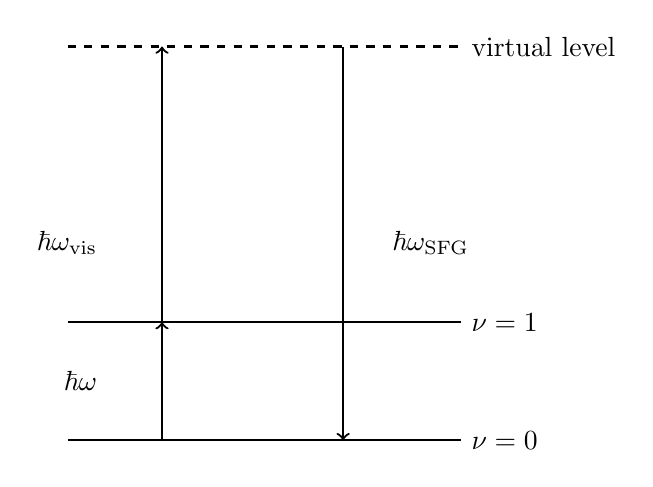
\begin{tikzpicture}[help lines/.style={thin,draw=black!50}]
%%\draw[help lines] (0,0) grid (4,4);
\draw [-, thick] (0,0) -- (5,0) node [anchor = west] {$\nu =0$};
\draw (0.5,0.75) node [anchor = east] {$\hbar\omega$};
\draw [-, thick] (0,1.5) -- (5,1.5) node [anchor = west] {$\nu = 1$};
\draw (0.5,2.5) node [anchor = east] {$\hbar\omega_{\text{vis}}$};
\draw [-, thick,dashed] (0,5) -- (5,5) node [anchor = west] {virtual level};
\draw (4.0,2.5) node [anchor = west] {$\hbar\omega_{\text{SFG}}$};
\draw [->, thick] (1.2,0) -- (1.2,1.5);
\draw [->, thick] (1.2,1.5) -- (1.2,5);
\draw [->, thick] (3.5,5) -- (3.5,0);
\end{tikzpicture}
\caption{The schematic diagram of the VSFG process which involves IR and Raman transitions. The $\nu =0$, $\nu=1$ levels denote the ground and the first excited state of the oscillator\cite{Gang202104}, respectively.
 The dashed line denotes a virtual electronic state in the Raman transition.
}\label{fig:sfg_1a} 
\end{figure}
%
Because experiments usually employed visible and the VSFG frequencies are far from resonant 
conditions, $\chi^{(2),\text{NR}}$ can be considered totally off-resonant and therefore 
insensitive to the laser beams' frequencies involved. Therefore, we can neglect the 
frequency dependence of the non-resonant term.
The molecular information is contained in the resonant signal. The resonant susceptibility $\chi^{(2),\text{R}}(\omega)$ is given by 
\begin{equation}
  \chi_{\eta\xi\kappa}^{(2),\text{R}}(\omega)=\frac{-i}{\hbar}\int_0^\infty dt e^{i\omega t} \text{Tr}{[\rho,\mu_\kappa]\alpha_{\eta\xi}(t)},
\label{eq:chi_R}
\end{equation}
where the index ($\eta$, $\xi$ or $\kappa$) is one of $x, y$ and $z$ labels of the laboratory coordinate frame.
In Eq.\thinspace(\ref{eq:chi_R}) $\rho=e^{-\beta H}/Z$ for a system with Hamiltonian $H$ and partition function $Z$ at reciprocal temperature $\beta=1/k_\text{B}T$;
$\mu_\kappa$ is the $\kappa$-th component of the system electric dipole and ${\alpha_{\eta\xi}}$ is the $\eta\xi$-th component of the polarizabiltiy tensor\cite{1995SM}.
Besides the vibrational resonance, $\chi^{\text{(2),R}}$, which reflects the vibrational and orientational characteristics of the surface species, 
the VSFG signal also includes the contribution from the non-resonant signal background $\chi^{\text{(2),NR}}$, 
due to static hyperpolarizability of the interface itself\cite{CheM2012}.  
For example, there are strong non-resonant second-order nonlinear responses\cite{Pradier11,Vanselow2012,Wieckowski99} of the interface in the case of some metal(-oxide). 
Generally, experiments employ visible light and VSFG frequencies far from resonant conditions, therefore, the non-resonant 
term $\chi^{\text{(2),NR}}$ is approximately off-resonant to the light frequencies involved\cite{Morita2002}.
%Neglecting the frequency dependence of the nonresonant term $\chi^{\text{(2),NR}}$ is usually a good approximation. 

\paragraph{Microscopic expression of molecular hyperpolarizability} 
As the electric field is increased, the description of the induced dipole moment 
$\boldsymbol \mu$ should include the normally insignificant nonlinear terms. We can express the induced dipole moment as
\begin{equation}
  {\boldsymbol \mu} = {\boldsymbol \mu}_0 +\alpha {\bf E} + \beta {\bf E E}.
\label{eq:induced_mu}
\end{equation}
%or
%\begin{equation}
%  \mu_i = (\mu_0)_i +\alpha_i  E_i + \beta_{ijk}E_j E_k + \cdots.
%\label{eq:induced_mu}
%\end{equation}
The VSFG spectra are determined by the frequency-dependent hyperpolarizability in molecular level description. 
The frequency-dependent hyperpolarizability can be expressed as a sum of resonant and non-resonant terms:
\begin{equation}
\beta_{\eta\xi\kappa}(\omega_{\text{SFG}},\omega_{\text{vis}},\omega)=\beta_{\eta\xi\kappa}^{\text{R}}+\beta_{\eta\xi\kappa}^{\text{NR}},
\label{eq:beta}
\end{equation}
where $\eta$, $\xi$ and $\kappa$ are space-fixed axes.
The resonant term of the frequency-dependent hyperpolarizability is 
\begin{equation}
  \beta_{\eta\xi\kappa}^{\text{R}}(\omega_{\text{SFG}},\omega_{\text{vis}},\omega)=\sum_{v',v}\frac{\langle v|\alpha_{\eta\xi}|v'\rangle\langle v'|\mu_{\kappa}|v\rangle}{(\omega_{v'}-\omega_v)-\omega-i\gamma_{v'v}}\rho_v,
\label{eq:beta_R}
\end{equation}
where the subscripts $\eta$, $\xi$ and $\kappa$ denote body-fixed axes,
$\omega_{v'}-\omega_v$ is the vibrational energy gap, 
$\rho_v$ is the thermal distribution function of the initial vibrational states $v$,
$\alpha_{\eta\xi}$ is the $\eta\xi$-th component of the molecular dipole polarizability,
$\mu_{\kappa}$ is the $\kappa$-th component of the molecular dipole moment,
and $\gamma_{v'v}$ is the damping rate.
We can rewrite Eq.\thinspace(\ref{eq:beta_R}) as 
(Appendix \ref{calculation_of_chi}) 
\begin{align}
  \beta_{\eta\xi\kappa}^{\text{R}}&=i\int_0^\infty dt \sum_{v'v}e^{-i[(\omega_{v'}-\omega_v)-\omega-i\gamma_{v'v}]t} \langle v|\alpha_{\eta\xi}|v'\rangle\langle v'|\mu_{\kappa}|v\rangle \rho_v \nonumber\\
   &=i\int_0^\infty dt \sum_{v'v}e^{i\omega t} \langle v|e^{iHt}\alpha_{\eta\xi}e^{-iHt}|v'\rangle\langle v'|\mu_{\kappa}|v\rangle \rho_v \nonumber\\
   &=i\int_0^\infty dt e^{i\omega t} \langle\alpha_{\eta\xi}(t)\mu_{\eta\xi}(0)\rangle,
\label{eq:beta_R_b}
\end{align}
where $H$ is the Hamiltonian of the system without external field. 
Eq.\thinspace(\ref{eq:beta_R_b}) indicates that the resonant term $\beta_{\eta\xi\kappa}^{(2),\text{R}}$ is the FT 
of the quantity $\langle\alpha_{\eta\xi}(t)\mu_{\kappa}(0)\rangle$, i.e., the ensemble average of the time correlation function $\alpha_{}(t)\mu_{r}(0)$.
The damping rate $\gamma_{v'v}$ is not explicitly included in Eq.\thinspace(\ref{eq:beta_R_b}), because the dephasing is incorporated in the time development of the off-diagonal matrix elements 
of $\alpha_{\eta\xi}(t)$ and $\mu_{\kappa}(0)$.

The tensor elements $\chi^{(2),\text{R}}_{\eta\xi\kappa}$ is microscopically represented as the average sum of first-order hyperpolarizability of the constituent molecules $\beta$ in the space-fixed frame
\begin{align}
  \chi^{(2),\text{R}}_{\eta\xi\kappa} = \langle \sum_i^N \sum_{pqr} D_{\eta p}(\Omega_i) D_{\xi q}(\Omega_i) D_{\kappa r}(\Omega_i) \beta_{pqr}\rangle
\label{average_sum}
\end{align}
where $D(\Omega_i)$ is the direction cosine matrix of the $i$-th molecule, projecting $\beta$ onto the space-fixed frame\cite{Morita2000}.

%and evaluate it with the static hyperpolarizability, which can be calculated by an \abinitio Molecular Orbital (MO) package\cite{Morita2002}, 
%\begin{equation}
%        \beta_{\eta\xi\kappa}^{\text{NR}}=\sigma\beta_{\eta\xi\kappa}^{\text{static}},
%\label{eq:beta_NR}
%\end{equation}
%where $\sigma$ is the symmetry number among the indices $\eta$, $\xi$ and $\kappa$.
%\paragraph{Derive the value of $\sigma$}
%The frequency-dependent hyperpolarizability, $\beta(\omega_1,\omega_2,\omega_3)$, satisfies the following equation 
%\begin{equation}
%\label{eq:beta_condition}
%        P_p(\omega_1)=\sum_q\alpha_{pq}(\omega_1)E_q(\omega_1)+\sum_{qr}\beta_{pqr}(\omega_1,\omega_2,\omega_3)E_q(\omega_2)E_r(\omega_3)+\cdots
%\end{equation}
%where the suffices $p$, $q$ and $r$ range over $x$, $y$ and $z$, and $P_p(\omega_1)$ is the induced dipole moment at frequency $\omega_1$. The static polarizability and hyperpolarizability are defined as 
%\begin{equation}
%        \alpha_{pq}^{\text{static}}=(\frac{\partial P_p}{\partial E_q})_{E=0},\ \
%        \beta_{pqr}^{\text{static}}=(\frac{\partial^2 P_p}{\partial E_q \partial E_r})_{E=0}
%\label{eq:beta_condition}
%\end{equation}
%and thus the dipole moment in a static external electric field is expressed as 
%\begin{equation}
%        P_p^{\text{static}}=(P_p)_{E=0}+\sum_q\alpha_{pq}^{\text{static}}E_q+\frac{1}{2}\sum_{qr}\beta_{pqr}^{\text{static}}E_qE_r+\cdots,
%\label{eq:static_dipole_moment}
%\end{equation}
%where $(P_p)_{E=0}$ is the permanent dipole moment. From Eq. (\ref{eq:beta_condition}) and Eq. (\ref{eq:static_dipole_moment}), we obtain $\sigma=1/2$ in Eq. (\ref{eq:beta_NR}).

\paragraph{Fresnel Factors}
Because of screening and dipole-dipole coupling, the local electric fields felt by molecules is different from the macroscopic fields\cite{Vanselow2012}. 
The VSFG signal depends on the magnitude of the local electric fields of the interacting optical beams at the interfaces. 
While the magnitude of the local electric fields is related to both the intensity of the incident beams and the linear refractive indices 
of the different layers (bulk) of the sample\cite{Khatib2016}. Fresnel coefficients define the magnitude of the electric fields at the interface. 
Therefore, to find out the magnitude of the local electric fields, we need to evaluate Fresnel factors. 
The VSFG intensity $I_{\text{SFG}}$, is proportional to the intensities of the incident visible and infrared beams, $I_{\text{vis}}$, $I$, 
and to the square of the second-order nonlinear susceptibilities,
$\chi_{\eta\xi\kappa}^{(2)}(\omega_{\text{SFG}})$, of the interface:
\begin{equation}
        \chi_{\eta\xi\kappa}^{(2)}(\omega_{\text{SFG}})\propto|\sum_{\eta,\xi,\kappa}L_{\eta\eta}(\omega_{\text{SFG}})\chi_{\eta\xi\kappa}^{(2)}(\omega_{\text{SFG}})L_{\xi\xi}(\omega_{\text{vis}})L_{\kappa\kappa}(\omega)|^2\text{sec}^2(\theta_{\text{SFG}})I_{\text{vis}}I
\label{eq:chi}
\end{equation}
where $\eta$, $\xi$, $\kappa$ are the Descartes coordinates of the reference frame;
$\omega_{\text{SFG}}=\omega_{\text{vis}}+\omega$ is the frequency of VSFG beam; 
$L_{\eta\eta}$, $L_{\xi\xi}$ and $L_{\kappa\kappa}$ are the Fresnel coefficients; 
$\theta_{\text{SFG}}$ is the reflected angle of VSFG beam with respect to the normal 
direction in the medium.

\subsection{VSFG spectra from velocity auto-correlation functions}
%To construct SFG spectrum of O-H stretching at the water/vapor interface and to ascertain the molecular origin of SFG spectrum, 
%quantum corrected time correlation function \cite{Morita2002,Morita2004} and instantaneous normal mode (INM) methods are used 
%by Perry and coworkers.\cite{Perry03} 
%For  water/vapor interface, the INM SFG spectrum is in agreement with the time correlatin function SFG spectrum. 
%This implies that motional narrowing effects play little role  in the interfacial line shape. The Shen group suggests that 
%the motional narrowing effects may be significant in the SPS geometry, where the "free O-H" stretching peak is greatly diminished.\cite{WeiX02}
%========================
%\section{solutions}
%Here we discuss the calculation of nonlinear susceptibility of water molecules at liquid/vapor interfaces.
%The SFG spectrum is proportional to the square of the nonlinear susceptibility of water molecules at the water/vapor interface. \cite{QD94}  
%Details:
This paragraph gives the derivation for the calculation of the sum frequency generation spectra of water interfaces that is
based on the projection of the atomic velocities on the local normal modes, such an approach permits one to obtain VSFG signals from suitable
velocity ACFs, reducing the computational cost to that of the accumulation of a molecular dynamics trajectory, and therefore cutting 
the overhead costs associated with the explicit calculation of the dipole and polarizability tensor. Moreover, the method permits to interpret 
the peaks in the spectrum in terms of local modes.
Components of the resonant term $\chi^{\text{(2),R}}_{\eta\xi\kappa}$ of the second order susceptibility can be calculated 
according to the classical formula\cite{Morita2002,Morita2008,Nihonyanagi2011}
\begin{align}
  \chi^{\text{(2),R}}_{\eta\xi\kappa}&=\frac{-i}{k_{\text{B}}T \omega} \int_0^\infty dt e^{i\omega t}\left\langle \dot{A}_{\eta\xi}(t) \dot{M}_{\kappa}(0)\right\rangle 
 \label{eq:chi}
\end{align}
%\begin{align}
% \chi^{(2)}_{XXZ,R}&=\frac{i}{k_BT \omega} \sum\limits_j \int_0^\infty dt e^{i\omega t} \left \langle \frac{\partial A_{XX}}{\partial r_j} \frac{\partial M_Z}{\partial r_j}  \dot{r}_j(0) \dot{r}_j(t) \right\rangle
% \label{eq:chi2}
% \end{align}
where $k_{\text{B}}$ is the Boltzmann constant, $\omega$ is the frequency of the IR beam, ${\bf M}$ (${A}$) is the dipole 
moment (dipole polarizability) of the system, and $\left\langle\dots\right\rangle$ denotes the average over all starting time points. 
%The derivation of Eq.\thinspace(\ref{eq:chi}) is given in Appendix \ref{calculation_of_chi}.
 
 The total dipole moment and dipole polarizability derivatives for the system can be expressed in terms of the water and bond contributions:
\begin{align}
 \dot{A}&=\sum_{i=1}^N \sum_{\epsilon}\dot{\alpha}^{i,\text{l},\epsilon} \\ 
 \dot{{\bf M}}&=\sum_{i=1}^N \sum_{\epsilon}\dot{\mu}^{i,\text{l},\epsilon} 
 \label{eq:A-M}
\end{align}
where ${\mu}^{i,\text{l},\epsilon}$ (${\alpha}^{i,\text{l},\epsilon}$) is the dipole moment (polarizability)
of the bond $\epsilon$ of the $i$-th water molecule, the superscript (l) denote these quantities are measured in the 
lab frame, and $N$ is the total number of water molecules.
Therefore, the correlation function in Eq.\thinspace(\ref{eq:chi}) can be written as 
\begin{align}
  \langle\dot{A}_{\eta\xi}(t)\dot{M}_{\kappa}(0)\rangle 
    &=\sum_{i=1}^N \sum_{\epsilon}\left\langle\dot{\alpha}_{\eta\xi,i,\epsilon}^{\text{l}}(t)\dot{\mu}_{\kappa,i,\epsilon}^{\text{l}}(0)\right\rangle \nonumber \\ 
    &+\sum_{i=1}^N \sum_{\epsilon}\left\langle\dot{\alpha}_{\eta\xi,i,\epsilon}^{\text{l}}(t)\dot{\mu}_{\kappa,i,-\epsilon}^{\text{l}}(0)\right\rangle \nonumber \\
    &+\sum_{i,j=1;i\neq j}^N \sum_{\epsilon,\epsilon'}\left\langle\dot{\alpha}_{\eta\xi,i,\epsilon}^{\text{l}}(t)\dot{\mu}_{\kappa,i,\epsilon'}^{\text{l}}(0)\right\rangle.
 \label{eq:correl_AM}
 \end{align}
In Eq.\thinspace(\ref{eq:correl_AM}), the first term of the right-hand side is the bond auto-correlation, the second term accounts 
for the correlation between the two bonds in the same water molecule, and the third them for the correlation between 
bonds in two different water molecules.
 
We assume that the bond elongation are small compared to the total bond length and stretching frequencies of the bond are 
much larger than frequencies of bond reorientation, for example, the libration.
Therefore, we can approximately write ${\dot\mu}(0)$ by 
\begin{align}
    \dot\mu_{\kappa}(0)&=\sum_i^{x,y,z}{{D}}_{\kappa i}(0)\dot{\mu}_i(0) \nonumber \\
                       &=\sum_i^{x,y,z}{{D}}_{\kappa i}(0)\biggl(\sum_j^{x,y,z}\frac{d\mu_i}{d r_j}\frac{d{r}_j}{dt}|_{t=0}\biggr) \nonumber \\
                       &=\sum_{i}^{x,y,z}{{D}}_{\kappa i}(0)\frac{d\mu_i}{dr_z}v_z(0),
    \label{eq:dot_mu}
 \end{align}
where ${D}_{\kappa i}$ is the direction cosine between the laboratory-fixed $\kappa$ axis and the molecular-fixed $i$ axis,
and $v_z=\frac{d{r}_z}{dt}|_{t=0}$ is the projection of the velocity on the bond axis.

Similarly, for the dipole polarizability, we have
\begin{align}
  \dot\alpha_{\eta\xi}(t)&=\sum_{i,j}^{x,y,z} \biggl({D}_{\eta i}(t)\frac{\partial\alpha_{ij}}{\partial r_z}{D}_{\xi j}(t)\biggr)v_z(t). 
  \label{eq:dot_alpha}
 \end{align}
The Eq.\thinspace(\ref{eq:dot_mu}) and Eq.\thinspace(\ref{eq:dot_alpha}) simplify the calculation of the  
$\left\langle \dot{A}_{\eta\xi}(t) \dot{M}_{\kappa}(0)\right\rangle$ in Eq.\thinspace(\ref{eq:chi}), because $v_z(t)$
and ${D}(t)$ can be readily determined from the DFTMD
trajectory, and $\frac{d\mu_i}{dr_z}$ and $\frac{d\alpha_{ij}}{dr_z}$ can be parameterized\cite{Corcelli2005,Khatib2016}.
%
\begin{figure}[H]
\centering
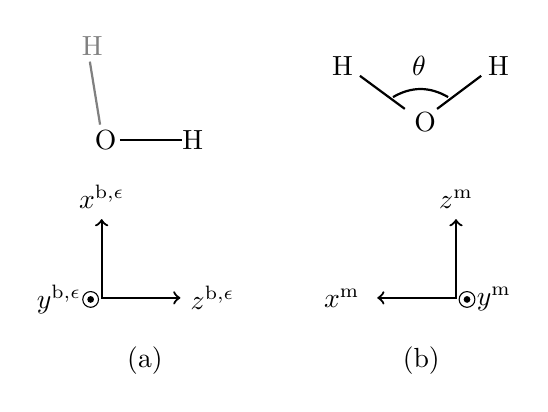
\begin{tikzpicture}[help lines/.style={thin,draw=black!50}]
%\draw[help lines] (0,0) grid (4,4);
%a
\draw [<->,thick] (0,1) node (xaxis) [above] {$x^{\text{b},\epsilon}$}
  |- (1,0) node (zaxis) [right] {$z^{\text{b},\epsilon}$};
  \filldraw[black] (-0.14,-0.02) circle (1pt) node [anchor=east] {$y^{\text{b},\epsilon}$};
\draw(-0.14,-0.02) circle (0.1);
\draw (0.2, -0.8) node [anchor=west] {(a)};
% H2O
\draw[gray,thick] (-0.02, 2.2) coordinate (a_1) -- (-0.15, 3) coordinate (a_2);
\draw[thick] (0.23, 2) coordinate (b_1) -- (1.02, 2) coordinate (b_2);
\draw (0.31, 2) node [anchor=east] {O};
\draw (0.9, 2) node [anchor=west] {H};
\draw[gray] (-0.12, 2.95) node [anchor=south] {H};
%\draw (0.56, 2.61) node {\chemfig{[:-84]H-O-[:0]H}};
%b
\draw [<->,thick] (3.5,0)--(4.5,0) node (xaxis){} 
  |- (4.5,0)--(4.5,1) node (zaxis) [above] {$z^{\text{m}}$};
  \filldraw[black] (4.64, -0.02) circle (1pt) node [anchor=west] {$y^{\text{m}}$};
\draw (2.7, 0) node [anchor=west] {$x^{\text{m}}$};
\draw(4.64,-0.02) circle (0.1);
\draw (3.7, -0.8) node [anchor=west] {(b)};
% H2O
\draw[thick] (3.85, 2.4) coordinate (a_1) -- (3.28, 2.82) coordinate (a_2);
\draw[thick] (4.26, 2.4) coordinate (b_1) -- (4.82, 2.82) coordinate (b_2);
\draw[thick] (3.7,2.55) to [out=30,in=150] (4.4,2.55);
\draw (4.03, 2.7) node [anchor=south] {$\theta$};
\draw (4.37, 2.23) node [anchor=east] {O};
\draw (5.04, 2.7) node [anchor=south] {H};
\draw (3.06, 2.7) node [anchor=south] {H};
%\draw (4.06, 2.61) node {\chemfig{[:-37]H-O-[:37]H}};
\end{tikzpicture}
  \caption{\label{fig:frameworks} The representation of the bond (a) and the molecular (b) frameworks\cite{Khatib2017}.}
\end{figure}

%
We used three different frameworks: the lab framework ($x^{\text{l}},y^{\text{l}},z^{\text{l}}$), the molecular framework 
($x^{\text{m}},y^{\text{m}},z^{\text{m}}$) and the bond framework ($x^{\text{b}},y^{\text{b}},z^{\text{b}}$) (Fig.\thinspace\ref{fig:frameworks}).
In the lab framework, the $z^{\text{l}}$-axis is perpendicular to the interface. 
The molecular frame will be used to decompose the signal into normal modes of water monomers. 
For the $j$-th molecule, the $z^{\text m}$ axis is along the bisector of the H-O-H angle, the $x^{\text m}$ axis is in the molecular plane, 
and the $y^{\text m}$ axis is out of the molecular plane\cite{Khatib2017}. 

In the bond framework, $z^{\text{b},\epsilon}$ axis is along the bond $\epsilon$ of a molecule, $z^{\text{b},\epsilon}$
is in the molecular plane and $y^{\text{b},\epsilon}$ is out of the molecular plane.
\begin{align}
  \dot{\alpha}^{\text{l},\epsilon} &= {{D}}^{\text{m}}{{D}}^{\text{b},\epsilon}(\frac{\partial{\alpha}^{\text{b}}}{\partial r}\dot
    r^{\epsilon})({D}^{\text{b},\epsilon})^{\text{T}}({D}^{\text{m}})^{\text{T}}, \\ 
    \dot\mu^{\text{l},\epsilon} &= {{D}}^{\text{m}}{{D}}^{\text{b},\epsilon}(\frac{\partial \mu^{\text{b}}}{\partial r}\dot r^{\epsilon}).
    \label{eq:dot_mu-alpha}
 \end{align}
The direction cosine matrix ${{D}}^{\text{b},\epsilon=1}$ and ${{D}}^{\text{b},\epsilon=-1}$ can be expressed as 
\begin{equation}
    {{D}}^{\text{b},1}=\left(
                \begin{matrix}
                    \text{cos}\frac{\theta}{2} &  0  & -\text{sin}\frac{\theta}{2}\\
                    0 & 1 & 0\\
                    \text{sin}\frac{\theta}{2} & 0 & \text{cos}\frac{\theta}{2}
\end{matrix}
\right),\quad
    {{D}}^{\text{b},-1}=\left(
         \begin{matrix}
             -\text{cos}\frac{\theta}{2} & 0 & \text{sin}\frac{\theta}{2}\\
             0 & 1 & 0\\
             \text{sin}\frac{\theta}{2} & 0  & \text{cos}\frac{\theta}{2}
\end{matrix}
\right),
\label{eq:D_b}
\end{equation}
where $\theta$ is the H-O-H angle in a water molecule.
%The approximate value of the angle is 105.5$^\circ$.
We use ${{D}}^{\text{m}}$ to transform the coordinates in a molecular framework to coordinates in the lab framework. 
Because the orientation of water molecules is changing during the simulation, 
%the angle $\theta'_i$ between the water dipole moment and the $z$-axis is time dependent, therefore, 
${{D}}^{\text{m}}$ is time dependent. 
%It can be expressed as 
%\begin{equation}
%    {\bf{D}}^{\text{m}}=
%    \left(
%        \begin{matrix}
%            \text{cos}{\gamma} & \text{sin}{\gamma} & 0\\
%            -\text{sin}{\gamma} & \text{cos}{\gamma} & 0\\
%            0 & 0 & 1
%        \end{matrix}
%     \right)
%     \left(
%         \begin{matrix}
%             \text{cos}{\theta'} & 0 & -\text{sin}{\theta'}\\
%             0 & 1 & 0\\
%             \text{sin}{\theta'} & 0  & \text{cos}{\theta'}
%         \end{matrix}
%     \right) 
%     =
%     \left(
%         \begin{matrix}
%             \text{cos}{\gamma}\text{cos}{\theta'} & \text{sin}{\gamma} & -\text{cos}{\gamma}\text{sin}{\theta'}\\
%             -\text{sin}{\gamma}\text{cos}{\theta'} & \text{cos}{\gamma} & \text{sin}{\gamma}\text{sin}{\theta'}\\
%             \text{sin}{\theta'} & 0  & \text{cos}{\theta'}
%         \end{matrix}
%     \right),
%\label{eq:D_m}
%\end{equation}
%where $\gamma$ is the angle between the incident plane (x-z plane) and the molecular plane of a water molecule,
%and $\theta'$ is the angle of the dipole moment of the water molecule from the normal direction of the interface, 
%and both $\gamma$ and $\theta'$ are time dependent.

Based on DFTMD simulations, we can implement the parameterization of $\frac{\partial \mu_{k}}{\partial r_z}$ and $\frac{\partial\alpha_{ij}}{\partial r_z}$
and calculate the correlation function $\langle\dot{A}_{\eta\xi}(t)\dot{M}_{\kappa}(0)\rangle$ through the velocity ACF. 
This approximation for estimating the susceptibility retains the details of the interface, including the full electronic structure. 
And it reduces the computational cost for a total calculation with the instantaneous evaluation of the molecular dipoles and polarizabilities\cite{Sulpizi2013}. 
The parametrization of $\frac{\partial \mu_{k}}{\partial r_z}$ and $\frac{\partial\alpha_{ij}}{\partial r_z}$ is based 
on the calculation of the MLWF\cite{Marzari1997} 
 and can be done through the approach developed by Salanne \etal\cite{Salanne08} and Khatib \etal\cite{Khatib2017}.
The implementation of this parametrization is given in Appendix \ref{calculate_derivatives}.
%\paragraph{Calculation of $\chi^{(2)}$ (Method 2)}
%We now consider the velocities projection on the water normal modes, identified by the collective variables ${\bf{R}}_j$ in the molecular framework. 
%The single water molecule has nine normal modes. Six of them have the angular frequencies $\omega$ equal zero and three normal modes remains. 
%The three normal modes are the symmetric stretching (SS), the antisymmetric stretching (AS) and the bending (B).
%The dipole moment and the molecular polarizability of the $i$th water molecule can be rewritten as
%\begin{align}
%    \dot{\bf \alpha}_{i}^{\text{l}}(t)&={\bf{D}}_{\text{m},i}(\sum_{j=Q,SS,AS}\frac{\partial{\bf\alpha}_{i}^{\text{m}}}{\partial R_j}){\bf{D}}^{\text{T}}_{\text{m},i}, \\ 
%    \dot{\bf \mu}_{i}^{\text{l}}&={\bf{D}}_{\text{m},i}(\sum_{j=Q,SS,AS}\frac{\partial{\bf\mu}_i^{\text{m}}}{\partial R_j}\dot{R}_j).  
%    \label{eq:dot_mu_alpha}
%\end{align}
%where $i$ denote the $i$-th water molecule.


\section{Definitions of HB population and correlation functions}\label{section:def_HBP}
Luzar and Chandler\cite{AL96} have pioneered the analysis of HB dynamics of pure water, and
subsequently such analysis has been extended to more complex systems, e.g., electrolytes\cite{Chandra2000}, proteins\cite{Tarek02,Matthias13}, 
biomolecules\cite{Kolano06} and micellar surfaces\cite{SP05}.
There are geometric\cite{Kumar2007} and energetic\cite{Sciortino1989} criteria to define a HB.
Here we use the geometric one:
Two water molecules are H-bonded if their inter-oxygen distance between a specific tagged pair of water molecules 
is less than cutoff radius $r^{\text{c}}_{\text{OO}}$ and
the H-O$\cdots$O angle is less than cutoff angle $\phi^{\text{c}}$\cite{AKS86,JT90,SB02}. 
The value $r^{\text{c}}_{\text{OO}}$ corresponds to the first-minimum position of the O--O radial distribution function (RDF) of water\cite{Sciortino1989}.   
The choice for $\phi^{\text{c}}$ for water-water molecules is obtained by studying the average number of H-bonds,
as a function of $\phi^{\text{c}}$\cite{Luzar1993}. We call this definition of HB the acceptor-donor-hydrogen (ADH) criterion. 
To compare the impact of different HB definitions on HB dynamics, we also use another definition of HB in our analysis. 
When the distance between the oxygen atoms of two water molecules is less than $r^{\text{c}}_{\text{OO}}$, 
and the O-H$\cdots$O included angle is greater than cutoff angle $\theta^{\text{c}}$, then we say that there is a HB between the two molecules. 
We denote this definition as acceptor-hydrogen-donor (AHD) criterion.
In this thesis, we use $r^{\text{c}}_{\text{OO}}=3.5$ \AA both for the ADH and AHD criteria, $\phi^{\text{c}}=30^{\circ}$ for the ADH criterion, 
and $\theta^{\text{c}}=120^{\circ}$ for the AHD criterion.

% introduce h(t)
The configuration criterion above allows us to define a variable $h[r(t)] = h(t)$, the HB population. 
Here a configuration $r(t)$ denotes the positions of all the atoms in the system at time $t$\cite{AL96}.  
The $h(t)$ has a value 1 when the particular tagged pair of molecules are bonded, and 0 otherwise. 
%=================
% added 2020-5-27: to show that h(t) is actually the fluctuation of itself (\delta h).
The fluctuation or deviation in the dynamical variable $h(t)$ from its time-independent equilibrium average $\langle h\rangle$ , 
is defined by\cite{DC87} 
$$
\delta h = h(t) - \langle h\rangle.
$$
Since the probability that a specific pair of molecules is bonded in a large system is extremely small, i.e., 
the time average of $h$ is zero, or  
$\langle h \rangle = 0$,
then
$$
\delta h(t) = h(t).
$$
Therefore, $h(t)$ describe the fluctuation $\delta h(t)$  of the HB population.  
%=================

While the equilibrium average of $\delta h(t)$ is zero, we can obtain useful information by considering the equilibrium 
correlations between fluctuations at different times. The correlation between $\delta h(t)$ and $\delta h(0)$ can be written as 
$$
\langle \delta h(0) \delta h(t)\rangle = \langle h(0)h(t)\rangle-\langle h \rangle^2 = \langle h(0)h(t)\rangle,
$$
where the averaging $\langle\cdots\rangle$ is to be performed over the ensemble of initial conditions.% $(r^N, p^N)$.


In this paragraph, we use the following three correlation functions to describe the HB dynamics of the water/vapor interface:
the HB population ACF \CHB, the continuum HB population correlation function (also called survival probability) 
\SHB and the reactive flux $k(t)$\cite{Rapaport1983}.

\FloatBarrier
\paragraph{HB population ACF \CHB}\label{para:def_HBP}
The structural relaxation of H-bonds is described by the ACF \CHB of the HB population, i.e., 
\begin{eqnarray}
c(t)=\langle h(0)h(t) \rangle/\langle h\rangle
\label{eq:C_HB}.
\end{eqnarray}
With the aid of the ergodic principle, the ensemble average $\langle \cdots\rangle$ is implemented by the time average.
The $\langle h\rangle$ is the probability that a pair of randomly chosen water molecules in the system is
H-bonded at any time $t$. 
As examples, the dynamics of the inter-oxygen distance $r_{\text{OO}}(t)$, 
the cosine of the H$-$O$\cdots$O angle (cos$\phi(t)$)  
and the HB population operator $h(t)$ for a HB in a DFTMD simulated water cluster (H$_2$O)$_n$ (n=5) 
at 300 K is displayed in Fig.\thinspace\ref{fig:Ex30ps_hb}, respectively.
%-------------------
\begin{figure}[hbtp]
\centering
\includegraphics [width=0.7\textwidth] {./diagrams/Ex30ps_hb}
\setlength{\abovecaptionskip}{0pt}
\caption{\label{fig:Ex30ps_hb}Dynamics of $r_{\text{OO}}(t)$ (top panel), cos$\phi(t)$ (middle panel), 
  and $h(t)$ (bottom panel) for a typical HB in a water cluster. The dashed lines show the inter-oxygen distance 
  boundary $r^{\text{c}}_{\text{OO}}$=3.5 \AA (top panel) and criterion of cosine of H$-$O$\cdots$O angle cos$\phi^{\text{c}}$ 
  with $\phi^{\text{c}}$=30$^{\circ}$ (middle panel), respectively.}
\end{figure} 

In a large system that consists of many water molecules, the probability that a specific pair of water molecules are H-bonded is extremely small. 
Therefore, \CHB relaxes to zero when $t$ is large. 
The function \CHB measures correlation in $h(t)$ independent of any possible bond breaking events. 
It is one of the intermittent HB correlation functions, introduced by Stillinger, Rapaport 
and others\cite{Stillinger1975,Rapaport1983,Geiger1984,Zichi1986,Sciortino1989,Sciortino1990,Starr2000,vanderSpoel2006,Busch2021},
and can be studied by a continuous function, the probability density.
From \CHB, the HB relaxation time $\tau_{\text{R}}$ can be computed by
\begin{eqnarray}
  \tau_{\text{R}} &=& \frac{\int t c(t)\text{d}t}{\int c(t)\text{d}t}.
\label{eq:tau_relaxation}
\end{eqnarray}

The ACF \CHB for the simulated bulk water 
(for computational details see Appendix\thinspace\ref{DETAILS_NEAT_WATER})
is shown in Fig.\thinspace\ref{fig:pure_bk_c_from_2_methods} a. 
We can obtain the relaxation time from Eq.\thinspace\ref{eq:tau_relaxation}: $\tau_R = 14.01$ ps for the ADH definition, 
and $\tau_R = 14.16$ ps for the AHD definition. 
\begin{figure}[H]
\centering
\includegraphics [width=1.0\textwidth] {./diagrams/pure_bk_c_from_2_methods}
\setlength{\abovecaptionskip}{0pt}
\caption{\label{fig:pure_bk_c_from_2_methods}
The \CHB for bulk water, as computed from the ADH (solid line) and AHD (dashed line) criterion of H-bonds. 
	(a) The interchange processes are neglected;
	(b) the interchange processes are included. }
%\caption{\label{fig:128w_c_itp_bk_ns40}Time dependence of \CHB for bulk water at 300 K with density $\rho =1.00$ g/cm$^3$.} 
%The length of the trajectory is 35 ps of physical time. Ref:\cite{Khaliullin2013}}
\end{figure} 

The method of HB population-based HB dynamics has been frequently used in previous literature\cite{Luzar1994,AL96,Chandra2000}. 
The basis is the population operator $h(t)$ of the HB formed between two water molecules. 
The function \CHB is interpreted as the probability that the HB is intact at time $t$, 
if the pair of water molecules are H-bonded at time zero. 

%Besides $h(t)$, here we also discuss another possible definition of the HB population operator ${h}'(t)$.
When a pair of water molecules are H-bonded, 
there are 4 different forms of possible H-bonds . 
In other words, there are exchange processes, i.e., interchange tunneling and bifurcation tunneling, during the dynamics.
After an exchange process, a pair of bonded molecules still form H-bonds.
%we say that an old HB is broken and a new HB is formed.
In the above definition, we have not included this interexchange process, i.e., H-bonds before and after the interexchange process are regarded as the same HB.
After considering this interexchange process in the definition of HB population, the relaxation of the corresponding function $c(t)$ is slightly faster  
(Fig.\thinspace\ref{fig:pure_bk_c_from_2_methods} b),   
because the bifurcation tunneling (hydrogen exchange) is considered.
Besides, in Fig.s\thinspace\ref{fig:pure_bk_c_from_2_methods} a and \ref{fig:pure_bk_c_from_2_methods} b, 
we plotted \CHB for bulk water, using the ADH and AHD criteria of HB. We find that the relaxation time of H-bonds is not affected by the HB criteria. 
In the next paragraphs, for the sake of simplicity, 
we will ignore this interchange process and simply regard the H-bonds before and after the exchange process as the same HB.
%Fig.\thinspace\ref{fig:pure_bk_c_from_2_methods} a shows the correlation function \CHB for bulk water over time. 
%In the following, we will use the original HB population based on O--H bond, instead of water--water molecule pairs, unless otherwise specified.


Because the thermal motion can cause distortions of H-bonds from the perfectly tetrahedral configuration,
water molecules show a librational motion on a time scale of $\sim$ 0.1 ps superimposed to rotational and diffusional motions ($> 1$ ps), 
which causes a time variation of interaction parameters.
A new HB population $h^{(d)}(t)$ was also defined to obviate the distortion of real HB dynamics\cite{Sciortino1989,Chandra2000}.
The $h^{(d)}(t)$ is 1 when the inter-oxygen distance of a particular tagged pair of water molecules is less than $r^{\text{c}}_{\text{OO}}=3.5$ \AA at time $t$ and 0 otherwise. 
The difference between the operators $h^{(d)}(t)$ and $h(t)$ is that there is no restriction on the angle. Therefore, those molecular pairs that meet the condition of $h^{(d)}(t)=1$ may not meet the condition of $h(t)=1$.
That is, the H-bonds between the tagged molecular pairs that satisfy the condition $h^{(d)}(t)=1$ may have been broken, but they may more easily form H-bonds again.
The function 
\begin{eqnarray}
  c^{(d)}(t)=\langle h(0)h^{(d)}(t) \rangle/\langle h\rangle
\label{eq:C_HB_d}
\end{eqnarray}
is the probability that the specific two water molecules are located in reformable region ($r_{\text{OO}} < r^{\text{c}}_{\text{OO}}$) at time $t$,
if they were H-bonded at time zero. 
The time correlation function 
%
\begin{eqnarray}
n(t)=\langle h(0)[1-h(t)]h^{(d)}(t) \rangle/\langle h\rangle 
\label{eq:n_HB}
\end{eqnarray}
represents the probability at time $t$ 
that a tagged pair of initially H-bonded water molecules are not bonded but remain separated by less than $r_{\text{OO}}^{\text{c}}$,
$1-h(t)$ describes the breaking of a HB at time $t$ after its formation at time $t=0$.
The probability at time $t$ that a pair of water molecules bonded at the initial moment does not be bonded 
but the distance between their oxygen atoms is still less than $r_\text{OO}^c$ is calculated according to 
\begin{eqnarray}
n(t) = \int_0^t dt'k_\text{in}(t'),
\label{eq:n_from_k_in}
\end{eqnarray}
where $k_\text{in}(t) = -\langle \dot h(0)[1-h(t)]h^d(t) \rangle/\langle h\rangle$ is the restricted rate function. 
%===============================
\FloatBarrier
\paragraph{Continuum HB population correlation function \SHB}
%===============================
Another scheme to describe the HB dynamics is the continuum HB population correlation function \SHB, or survival probability\cite{Chandra2000} for a newly generated HB.
It is defined as
\begin{eqnarray}
s(t)=\langle h(0)H(t) \rangle/\langle h\rangle 
\label{eq:S_HB},
\end{eqnarray}
where $H(t)=1$ if the tagged pair of molecules, remains \emph{continuously} H-bonded till time $t$ 
and 0 otherwise.  It describes the probability that an initially H-bonded molecular pair 
remains bonded at all times up to $t$\cite{Chowdhuri2006}.
The \SHB for the simulated bulk water according to the formula \ref{eq:S_HB} is shown in Fig.\thinspace\ref{fig:128w_s_itp_bk_ns40}.
%
\begin{figure}[hbtp]
\centering
\includegraphics [width=0.60\textwidth] {./diagrams/128w_s_bk_ns40}
\setlength{\abovecaptionskip}{0pt}
\caption{\label{fig:128w_s_itp_bk_ns40} Time dependence of \SHB for bulk water.} 
%The length of the trajectory is 35 ps of physical time.
\end{figure} 

The average continuum HB lifetime $\langle \tau_{\mathrm{a}} \rangle$ is calculated by the integration of \SHB over $t$ (for detailed derivation see Appendix \ref{diff_distr}) :  
\begin{eqnarray}
  \langle\tau_{\mathrm{a}}\rangle = \int_0^\infty s(t) dt.
\label{eq:calculate_hb_lifetime_from_s}
\end{eqnarray}
%
The time derivative 
\begin{eqnarray}
P_a(t) = -\frac{\text{d}s(t)}{\text{d}t}\nonumber
\label{eq:P_1}
\end{eqnarray}
represents the first passage time probability density of H-bonds. $P_a(t)$ is also called probability distribution of HB lifetimes\cite{Sciortino1990prl,Krausche1992,FWS99,Voloshin2009}, or histogram of HB lifetimes\cite{Geiger1984,Stanley2000}.
It denotes the probability of the first HB breaking in time $t$ after it has been detected at $t=0$, i.e.,
\begin{eqnarray}
s(t)= \int_t^\infty P_a(t')dt'.
\label{eq:P_2}
\end{eqnarray}

\FloatBarrier
\paragraph{Reactive Flux $k(t)$} 
The rate of relaxation to equilibrium is characterized by the reactive flux correlation function, 
\begin{eqnarray}
k(t) = -\frac{\text{d}c(t)}{\text{d}t},
\label{eq:k}
\end{eqnarray}
i.e., $k(t)=\langle j(0)[1-h(t)]\rangle/\langle h\rangle$\cite{AL96,AL00},
where 
$j(0)=-\text{d}h/\text{d}t|_{t=0}$ 
is the integrated flux departing the HB configuration space at time $t=0$ (for detailed derivation see Appendix \ref{calc_rf}).
$-k(t)$ is the average rate of change of HB population for the trajectories in which the HB is broken at a time $t$ later\cite{AL96}, 
independent of possible breaking and reforming events in the interval from 0 to $t$.
Therefore, $k(t)$ measures the effective decay rate of an initial set of H-bonds\cite{DC87,Starr2000}.


Assuming that each HB acts independently of other H-bonds, 
from detailed balance condition, we obtain 
\begin{eqnarray}
  \tau_{\text{HB}} &=& \frac{1- \langle h\rangle}{k},
\label{eq:rate}
\end{eqnarray}
where $k$ is the rate constant of breaking a HB (forward rate constant)\cite{Chandler1986,Chandler1978}. 
For an aqueous interface, the probability that a given tagged molecule pair forms a HB is very low, i.e., $\langle h\rangle \ll 1$. 
Therefore, from Eq.\thinspace\ref{eq:rate}, $k$ is related to the average HB lifetime by $\tau_{\text{HB}}=1/k$.
Using $k'$ to represent the rate constant from the HB \emph{on} state to the HB \emph{off} state for a tagged pair of molecules (backward rate constant),
the reaction time constant $\tau_\text{re}$ is 
\begin{eqnarray}
  \tau_\text{re} &=& \frac{1}{k+k'}.\nonumber
\label{eq:reaction_rate_tau}
\end{eqnarray}

 
  \chapter{Alkali nitrate clusters}\label{CHAPTER_Clusters}
There are two ways of obtaining highly specific information on solvation structures: studying gas-phase clusters consisting of ions surrounded by a few water molecules\cite{Weber2000,Kropman2001},
and exciting and detecting a dissolved prob molecule\cite{Jimenez1994}.
Due to the experimental difficulties, most information on the dynamics of aqueous solvation shells was obtained from MD simulations\cite{Smith1994,Chandra2000}.
  In this chapter, DFTMD simulations of gas phase clusters including alkali metal cations, nitrate ions and a few water molecules have been used to obtain these specific information and to understand the
  effects of alkali cations and nitrate anions on H-bonding\cite{jiangling2010,heine2015}. 
  The VDOS is used to extract the vibrational signatures for water molecules in these systems.
  In Paragraphs \ref{paragraph_3w_nitrate} and \ref{paragraph_clusters_alkali_water}, 
  the effect of the anion and the cation are separately investigated. 
  The two clusters, [NO$_3\cdot$(H$_2$O)$_3$]$^-$ and [Li$\cdot$(H$_2$O)$_4$]$^+$, are used 
  to study the structural and dynamical properties of water clusters with nitrate ions and with alkali cations. 
  In Paragraph \ref{paragraph_clusters_alkali_nitrate_and_water_molecules}, the effects of alkali metal cations 
  and nitrate anion are discussed within clusters containing both cations and anions and an increasing number of water molecules.
  %
  \section{Cluster of nitrate and water molecules}\label{paragraph_3w_nitrate}
  %EXAMPLE of FORMULA
  %$$X_n=X_k \qquad\hbox{if and only if}\qquad Y_n=Y_k \quad\hbox{and}\quad Z_n=Z_k.$$
  
  %\begin{wrapfigure}{l}[0.05cm]{8.0cm}
  %\centering
  %\includegraphics[width=0.3\textwidth]{./diagrams/3_NO3_small}
  %\setlength{\abovecaptionskip}{10pt}
  %\caption{The geometry optimized structure of the cluster NO$_3^-$(H$_2$O)$_3$. The red dotted lines denote the H-bonds.}\label{fig:3_NO3_small}
  %\end{wrapfigure}
  \begin{figure}[H]
  \centering
  \includegraphics[width=0.7\textwidth]{./diagrams/clusters_4}
  \setlength{\abovecaptionskip}{0pt}
    \caption{\label{fig:clusters_4}Geometry optimized structure of clusters: 
    (a) [NO$_3\cdot$(H$_2$O)$_3$]$^-$; 
    (b) RNO$_3$(H$_2$O)$_3$; 
    (c) RNO$_3$(H$_2$O)$_4$; 
    (d) RNO$_3$(H$_2$O)$_5$ (R=Li, Na, K)
	  (for more structural properties see Appendix \ref{structure_of_clusters}).}
  \end{figure}
  First, we consider the nitrate--water cluster, [NO$_3\cdot$(H$_2$O)$_3$]$^-$. The symmetric isomer of the cluster, 
  as shown in Fig.\thinspace\ref{fig:clusters_4} a, is obtained by geometry optimization at the BLYP/TZV2P level of theory. 
  According to the definition of HB\cite{JT90,SB02}, there are three H-bonds in it,
  i.e., only one of the two OH bonds is H-bonded to \nitrate in each water molecule. 
  Therefore, the two OH bonds in each water molecule exhibit different vibrational features. 
  Fig.\thinspace\ref{fig:vdos_NO3-3w_2_H6H7} shows the VDOS for OH bonds in the cluster.
  For each water molecule, one OH bond is vibrating in the frequency range 3680--3700 cm$^{-1}$, 
  while the other in the range 3380--3440 cm$^{-1}$. 
  The difference of frequencies between these vibrational modes is about $\Delta\nu=$ 180 \centimeter.
  %
  \begin{figure}[H] %[htbp]
  \centering
  \includegraphics [width=0.5\textwidth] {./diagrams/vdos_NO3-3w_2_H6H7_simple}%
  \setlength{\abovecaptionskip}{0pt}
    \caption{\label{fig:vdos_NO3-3w_2_H6H7} The VDOS for the two OH bonds in w1 (Fig.\thinspace\ref{fig:clusters_4} a) of [NO$_3\cdot$(H$_2$O)$_3$]$^-$.} 
    %The length of the DFTMD trajectory is 5 ps.
  \end{figure}  %(Calculated from the function vdos3.f and ft$\_$5s.sh)
  %(MS:repetition)A quasi-HB is formed if the O--H distance $r_\text{OH}$ satisfies the condition $r_\text{OH}<3.5$ \AA, but not that the O--H$\cdots$O angle is less than $\frac{\pi}{6}$. \cite{JT90} 
  Additionally, we label the three water molecules as w1, w2, and w3, respectively (Fig.\thinspace\ref{fig:clusters_4} a). 
  For the three water molecules, we find some differences in the structural parameters.
  Table\thinspace\ref{tab:3_nitrate_bond} gives the calculated lengths of H-bonds in the cluster [NO$_3\cdot$(H$_2$O)$_3$]$^-$. 
  The average differences $\Delta{d}$ between the H-bonds and other three bonds are 0.69 \AA (Table\thinspace\ref{tab:3w_nitrate}). 
  %============
  %section 4_Li
  %============
  \section{Cluster of alkali metal cation and water molecules}\label{paragraph_clusters_alkali_water}
  \begin{wrapfigure}{l}[0.05cm]{6.5cm}
  \centering
  \includegraphics[width=0.25\textwidth]{./diagrams/4_Li}
  \setlength{\abovecaptionskip}{0pt}
  \caption{\label{fig:4_Li}The cluster [Li$\cdot$(H$_2$O)$_4$]$^+$.}
  \end{wrapfigure}
  %====
  To find the effects of alkali cations on the structural properties of water, we investigated the cluster \LiFourW 
  (Fig.\thinspace\ref{fig:4_Li}). We concentrate on two aspects: the radial distribution function (RDF), 
  and the VDOS for water molecules of this cluster.

  Sharp peaks in the RDF (Fig.\thinspace\ref{gdr_4_Li}) show that the solvation shell of \Li is bound to all the four water molecules.
  The peak for $g_{\text{LiO}}$ is at 2.02 \AA, and for $g_{\text{LiH}}$ is at 2.69 \AA. 

  %
  The VDOS for water molecules in the cluster [Li$\cdot$(H$_2$O)$_4$]$^+$ is calculated from a 20-ps trajectory,
  during which one water molecule escaped from the bonding of the Li and then formed a new HB to 
  another water molecule. Figure \thinspace\ref{fig:vdos_4_Li} A 
  shows that there are two types of OH stretching modes in the cluster \LiFourW:
  free OH stretch which peaks at 3705 \cm and bonded OH stretch at 3625 \centimeter. 
  However, water molecules just bound to Li has two degenerate free O-H stretching modes. 
  \begin{figure}[H] %[b!]
  \centering
  \includegraphics[width=0.60\textwidth] {./diagrams/gdr_4_Li}
  \setlength{\abovecaptionskip}{0pt}
    \caption{\label{gdr_4_Li}RDFs $g_{\text{Li-O}}$ and $g_{\text{Li-H}}$ for the cluster \LiFourW.} 
  \end{figure}
\begin{figure}[H]%
    \centering
    \subfloat[]{{\includegraphics[width=6.6cm]{./diagrams/vdos_4_Li} }}
    \qquad
    \subfloat[]{{\includegraphics[width=6.2cm]{./diagrams/vdos_4_Li-wat_w1_5ps} }}
    \caption{
(A) 
The VDOS for the four water molecules (all water molecules) in the cluster \LiFourW.
(B)
The VDOS for water molecules (three water molecules) bound to Li in the cluster \LiFourW.
}%
    \label{fig:vdos_4_Li}%
\end{figure}
  %
  The VDOS for water molecules only bound to Li (Fig.\thinspace\ref{fig:vdos_4_Li} B) shows that these water molecules only have free OH stretch, 
  since there is only a broad stretching mode at 3705 cm$^{-1}$.

  \section{Clusters of alkali nitrate and water molecules}\label{paragraph_clusters_alkali_nitrate_and_water_molecules}
  %===================
  %MS:INSERT AN INTRO:
  %===================
  As a first minimal model system for the interface of alkali nitrate solution, we consider alkali nitrate water clusters including 3 to 5 waters. 
  The idea is to investigate the effect of alkali nitrate on the vibrational properties of those water molecules which are directly 
  H-bonded to the ions.
  In our simulations, clusters are geometry optimized and the most stable configurations are determined (Fig.s\thinspace\ref{fig:clusters_4} b--d).
  The first interesting result is that for all the clusters containing 3 to 5 water molecules, a contact ion pair is maintained during the 
  simulation trajectories where a \emph{direct} interaction involves the cation and one of the nitrate oxygen's. 

In the LiNO$_3$(H$_2$O)$_3$ cluster, there are three H-bonds and three Li-O bonds. 
The average lengths of them are given in Table\thinspace\ref{tab:table_lino3}. 
We use HB1, HB2 and HB3 to denote the HB between w1 and w2, w2 and \nitrate, and w3 and \nitrate, 
respectively (Fig.\thinspace\ref{fig:clusters_4} b). Both the average lengths of HB1 and HB3 are very close 
to each other and both of them are smaller than that of HB2. 
Since both w1 and w3 are bound to \li, we calculate an average value $\bar{d}_{\text{HB}}=1.81$ \AA of the lengths of HB1 and HB3.
The difference between length of HB2 and $\bar{d}_{\text{HB}}$ is $\delta d_{\text{HB}}=0.19$ \AA.
By testing the difference of environment of each H-bonds,  we obtain that $\delta d_{\text{HB}}$ comes from the 
difference between Li-O bonds and H-bonds.
\begin{table}[htbp]
\centering
\caption{\label{tab:table_lino3}%
  The average length $r_a$ of H-bonds (Li-O bonds) in the cluster LiNO$_3$(H$_2$O)$_3$.}
\begin{tabular}{ccc}
Bonds& $r_a$( \AA) \\ 
\hline
HB1 &1.83 $\pm$ 0.14\\
HB2 &2.00 $\pm$ 0.25 \\
HB3 &1.79 $\pm$ 0.16 \\
O(w1)--Li &1.95 $\pm$ 0.09 \\
O(w3)--Li &1.92 $\pm$ 0.07 \\
nitrate O--Li &1.91 $\pm$ 0.08
\end{tabular}
\end{table}

%\subsection{Structural Characterization}
 Besides, the RDF between the alkali (\li, \na\space or \pot) and the water O (panel a) and the nitrate O (ON)-- water H (HW) (panel b) are reported in Fig.\thinspace\ref{fig:gdr_3_RNO3}. 
The sharp and left-shifted peaks (Fig.\thinspace\ref{fig:gdr_3_RNO3} b) 
show that the nitrate is solvated and in particular a stronger HB is formed in the presence of the cation in all three clusters. 
%=============
% To express number ranges like 2--4, use en-dash, which can be implemented by typing two hyphens (--).
%=============

 The vibrational features associated to these small clusters are calculated from the VDOS and reported in
Fig.\thinspace\ref{fig:vdos_Li_Na_K-NO3-3w}.
In the frequency range 3000--3800 \centimeter, each water molecule has two vibrational bands. In addition
to the free OH peak at $\sim$3700 \centimeter, we see that the H-bonded band (HB band) is characterized by quite strong \emph{red-shifted} 
peaks around 3200 \centimeter. These red-shifted peaks are associated to water molecules which are bound either to 
the cation or to both cation and anion and are different with respect to the peaks associated to the water molecules
which only bound to the nitrate in the cluster [NO$_3\cdot$(H$_2$O)$_3$]$^-$ (3430 \centimeter, see Fig.\thinspace\ref{fig:vdos_NO3-3w_2_H6H7}). 
%
%\egin{figure}[h!]
\begin{figure}[H]
\centering
  \includegraphics [width=\textwidth] {./diagrams/gdr_3_RNO3}
\setlength{\abovecaptionskip}{0pt}
\caption{\label{fig:gdr_3_RNO3} (a) RDF $g_{\text{R-O}}$ for clusters RNO$_3$(H$_2$O)$_3$ (R=Li, Na, K);
  (b) RDF $g_{\text{O-H}}$ for clusters RNO$_3$(H$_2$O)$_3$ and [NO$_3\cdot$(H$_2$O)$_3$]$^-$ (no alkali metal cation, denoted as "R=-").}
\end{figure}
%
\begin{figure}[H]
 \centering
 \includegraphics [width=1.1\textwidth, center] {./diagrams/vdos_Li_Na_K-NO3-3w}
 \setlength{\abovecaptionskip}{0pt}
  \caption{\label{fig:vdos_Li_Na_K-NO3-3w}The VDOS for H$_2$O in clusters: (a) LiNO$_3$(H$_2$O)$_3$, (b) NaNO$_3$(H$_2$O)$_3$ and (c) KNO$_3$(H$_2$O)$_3$.  
 w1: \water bound to R and \water;
 w2: H$_2$O bound to nitrate and \water;
 w3: \water bound to R and nitrate.
 } 
\end{figure}
%
\begin{figure}[H]
\centering
\includegraphics [width=1.1\textwidth, center] {./diagrams/vdos_LiNO3-3-5w}
\setlength{\abovecaptionskip}{0pt}
\caption{\label{fig:vdos_LiNO3-3-5w}The VDOS for H$_2$O in clusters LiNO$_3$(H$_2$O)$_n$: 
  (a) $n=3$;  (b) $n=4$; (c) $n=5$.
  w1: H$_2$O bound to Li and \water;
  w2: H$_2$O bound to nitrate and \water;
  w3: H$_2$O bound to Li and nitrate;
  w4: H$_2$O bound to \water;
  w5: H$_2$O only bound to Li.}
\end{figure}
%

To explore the effect of adding some additional water molecules to
the cluster, we considered clusters RNO$_3$(H$_2$O)$_n$ ($n$=4, 5; R=Li, Na, K).
The most stable configurations are shown in Fig.s\thinspace\ref{fig:clusters_4} c and d,
and the corresponding VDOS for water molecules are shown in
Fig.s\thinspace\ref{fig:vdos_LiNO3-3-5w} b and c for the clusters LiNO$_3$(H$_2$O)$_n$
($n$=4 and 5). We find that the OH stretching peaks in the HB region are also quite red-shifted.
The red shift is particularly strong for the water molecules which are directly interacting with
the Li and those which are simultaneously bound to the Li and to the nitrate O's (e.g. w3).

%

We also calculated the effects of other alkali metal cations, namely Na$^+$ and K$^+$. 
The calculated VDOS for water molecules in clusters NaNO$_3$(H$_2$O)$_3$ and KNO$_3$(H$_2$O)$_3$ are shown in 
Fig.s\thinspace\ref{fig:vdos_Li_Na_K-NO3-3w} b and c, respectively. As in the case of LiNO$_3$(H$_2$O)$_3$, the HB 
bands are also characterized by red-shifted peaks around 3200 \centimeter.
In addition, the peaks in the OH-stretching region are also compatible with infrared predissociation
(IRPD) spectra which have been recorded for the [Li$\cdot$(H$_2$O)$_{3-4}$Ar]$^+$
clusters\cite{rodriguez2011, Miller2008, Miller2008b}
and for [Na$\cdot$(H$_2$O)$_{4-7}$]$^+$ and [K$\cdot$(H$_2$O)$_{4-7}$]$^+$ clusters\cite{beck2011}, although there no
nitrate is present and only the effect of the cation was investigated.
%	
\section{Summary}
To summarize, the vibrational spectra from the clusters clearly point to red-shifted peaks which are not 
recorded in VSFG spectra at the solution/vapor interface for the \LiN solution. 
In other words, these clusters are not really representative of the solvation structures presents in the \LiN solution.
Therefore, these small clusters cannot be directly used to describe the topmost layer of the \LiN solution, 
and we need to build more realistic models to capture main features of the interface. 
In particular, according to the cluster picture one would be tempted to rule out the possibility of a contact 
ion pair at the interface.

 
\chapter{VSFG spectroscopy of the water/vapor and solution/vapor interfaces}\label{CHAPTER_SFG}
In Chapter \ref{CHAPTER_Clusters}, we investigated the VDOS for water clusters containing nitrate and alkali metal ions.
We found that small clusters cannot be directly used to model interfaces of aqueous solutions,
and we need to build more realistic ones to capture the main features of interfaces.
In this chapter, we will analyze the structure and dynamics of solutions containing an alkali cation and a nitrate (iodide) ion and to provide 
a microscopic interpretation of recent experimental results\cite{Salvador2003,Jubb2012,HuaWei2014}. 

The goal of this chapter is to find the origin of the main characteristics of the VSFG spectrum of the \LiN solution,
and provide a molecular picture to interpret the recorded spectra.
To achieve this goal, we simulate a solution/vapor interface including \Li and \nitrate
(Fig.\thinspace\ref{fig:interface_chandler}),
and extract the vibrational spectroscopic properties of the interface.
%=========
\begin{figure}[htbp]
\centering
\includegraphics [width=0.7 \textwidth] {./diagrams/interface_chandler}
\setlength{\abovecaptionskip}{0pt}
\caption{\label{fig:interface_chandler} The salty water interface of \LiN solution (left, top) and the water/vapor interface (left, bottom). 
The right panel shows that the \Li and the \nitrate ions are separated by a water molecule at the salty interface.}
\end{figure}

We consider a model for the interface where a slab of 256 water molecules containing one \Li and 
one \nitrate (LiNO$_3$(H$_2$O)$_{256}$) is included in a periodic simulation box of 19.70 $\times $ 19.70 $\times $ 40.00 \A$^3$ at 300 K.
The slab is 20 \AA thick and infinite in the \X and \Y direction, while the
separation between the periodic slabs in the \Z direction is 20 \A.
The  \LiN was inserted at one of the two interfaces, with the \nitrate residing in the topmost layer and 
the \Li residing somewhat deeper at about 5 \AA from the surface. In this way we have a model with one \emph{salty} interface
and one \emph{neat} interface which can be used as a reference.  
To provide the interpretation to the above experimental results, the following analysis tools are used:
(1) VDOS; 
(2) calculation of the nonlinear susceptibility; 
(3) reconcile of the interface and cluster picture.
In Paragraph \ref{sfg_ln}, the VSFG spectrum of the alkali nitrate interface of  aqueous solutions is calculated,
to find the connection between these two kind of models: the interface and cluster picture.
Additionally, to study the effect of cations, interfaces of alkali iodide solutions are also studied in Paragraph \ref{sfg_alkali_iodide_interface}.

\section{VSFG spectra of the lithium nitrate solution/vapor interface}\label{sfg_ln}
% MAIN STATEMENT p1: LiNO3 forms a stable water separated ion pair at the interface.
% p1a: NO3- is on the surface.
It has been often put forward the idea that in nitrate solution anion and cation are paired 
at the interface and form a double layer. Based on the relatively high propensity of \nitrate for the interface\cite{Otten2007}
we decided to start DFTMD simulations with the anion at the water surface and to investigate the possibility that  \LiN
forms a stable water-separated ion pair at the interface. The idea that nitrate ions form water-separated pair where
the Coulomb interaction is shielded was already suggested for divalent cation nitrate\cite{XuM2009}.
%An equilibration time of about 10 ps was considered before the trajectory analysis, and subsequently 40 ps have been considered for production. 
The first result is that
such model system is stable and the \nitrate remains within the topmost water layer during all the simulation time.
This result can be found in the probability distribution along $z$-axis of the simulation box (Fig.\thinspace\ref{fig:prob_LiNO3-wat--256_LiNO3_double_axis}).
This is in agreement with previous simulation results based on polarizable classical force field\cite{DJT13}
and also with some DFTMD work on nitric acid, which was also found stable at the interface\cite{Shamay2007}. 
Moreover, the \Li remains relatively close to the surface, in a water sub-layer forming a water separated ion pair 
with \nitrate at the interface.
%
\begin{figure}[H]
\centering
\includegraphics [width=0.6\textwidth] {./diagrams/prob_LiNO3-wat--256_LiNO3_double_axis} 
\setlength{\abovecaptionskip}{0pt}
\caption{\label{fig:prob_LiNO3-wat--256_LiNO3_double_axis}Probability distributions of ions and water molecules for 
\LiN water interface along the normal direction.}
%During the simulation, the \Li is located in the middle layers of the system.  Thus, the effects of \Li on susceptibility of the water molecules is canceled. 
\end{figure}
%
% p2: The interface LiNO3 has depletion in 3200 cm-1 in SFG
% p1 => p2
We have calculated the nonlinear susceptibility for the two interfaces, namely the one containing the \LiN pair (salty interface) 
and the neat one which does not include any ion. 
The calculated imaginary part is reported in panel a and the intensity in panel b of  
Fig.\thinspace\ref{fig:sfg_LiNO3_7A_20ps_gauss150}. The calculated intensity spectra show a depletion of 
the 3200 \cm region as in the experiments (Fig.\thinspace\ref{fig:Allen12}).
The same feature is also shown in the imaginary part. 
Also the calculated spectra show that the free OH region is less intense in the salty interface with respect to the water/vapor interface.
%
\begin{figure}[H]
\centering
\includegraphics [width=\textwidth] {./diagrams/sfg_LiNO3_7A_20ps_gauss150}
\setlength{\abovecaptionskip}{0pt}
  \caption{\label{fig:sfg_LiNO3_7A_20ps_gauss150} (a) The $\Im\chi^{(2),\text{R}}_{SSP}$ and (b) $|\chi_{SSP}^{(2),\text{R}}|^2$ for water molecules 
at the interface of \LiN solution.} 
\end{figure}
\begin{figure}[H] %[htbp]
\centering
  \includegraphics [width=0.6 \textwidth] {./diagrams/vsfg_alkali_nitrate}
\setlength{\abovecaptionskip}{0pt}
  \caption{\label{fig:Allen12}Experimental VSFG intensity of \LiN solutions, compared with that of neat water\cite{HuaWei2014}.}
\end{figure}
%The simulation time is 40 ps and the $d$=9 \A. 
%Note:
%The simulation system is \Li ion, 1 \nitrate ion, and 256 water molecules in 19.7 $\times $ 19.7 $\times $ 40.0 \A$^3$ simulation box.

To find the microscopic origin of the depression of the lower frequency region,
we have also decomposed the salty water interface VDOS into the contributions coming from the different water molecules. 
%======================================================VDOS========================
%{Discuss the difference between the two interfaces using the VDOS--- Lore Sulpizi}
%To explore the ion-induecd effect in the interface, 
The VDOS $g_z(\nu)$ for the water molecules at the interface, which is calculated from the FT of atoms' ACF 
of velocity in the $z$-axis projection, gives a rough value of the thickness $d$ of the interface. 
Using 1, 2 and 5 \AA thicknesses, we have defined three different interfacial regions. 
For the LiNO$_3$ solution, $g_z(\nu)$ of the salty and neat water interfaces in the slab is reported in Fig.\thinspace\ref{fig:surf_x-vs-l_x_d1-5}.
When $d$ is equal to 1 \A, water molecules at the solution surface have lower free OH stretching frequency than that in pure water.
This means that there are less water molecules with free OH stretch at the interface of \LiN solution than at the water/vapor interface. 
It compares very well with the experimental result of the surface propensity of nitrate anions in water solution\cite{Salvador2003}.
Meanwhile, compared to the result of the water/vapor interface, the H-bonded band of the VDOS for the salty interface has a blue shift of $\Delta\nu\approx 80$ \centimeter.
As we increase the value of $d$, the difference between the VDOS of the water/vapor and solution/vapor interface is gradually reduced. 
When $d$ is equal to 2 \A, the amount of blue shift $\Delta\nu$ reduces to 55 \centimeter (Fig.\thinspace\ref{fig:surf_x-vs-l_x_d1-5} b); 
when $d$ is 5 \A, $\Delta\nu$ is almost zero (Fig.\thinspace\ref{fig:surf_x-vs-l_x_d1-5} c).
This tendency indicates that ions' (\li, \na, \K and \nit) effects 
can be found only on the water molecules in the top $\sim$5-\AA layer of the interface.
% p3: l=1A, peak of g_z for the interface is blue-shifted.
As the thickness of the interfacial water layer included in $g_z(\nu)$ increases, the free OH signal is depressed
and at the same time the H-bonded OH bands for the salty and neat water interfaces become more similar.
%To check the convergence of the dynamics of the system, $g_z(\nu)$ is calculated for the first half 10 ps 
%and the later half second 10 ps, respectively. (see Fig.\ref{fig:FT_all_w_in_interf})
\begin{figure}[H]
\centering
\includegraphics [width=0.6 \textwidth] {./diagrams/surf_x-vs-l_x_d1-5}
\setlength{\abovecaptionskip}{0pt}
\caption{\label{fig:surf_x-vs-l_x_d1-5}The VDOS $g_z(\nu)$ for water molecules at the interface of LiNO$_3$ solution 
  (solid line) and at the water/vapor interface (dashed line). (a): $d=1$ \A; (b): $d=2$ \A; (c): $d=5$ \A.}
\end{figure}
%

To explore the reason for the blue shift of the H-bonded OH stretch at the interface,
we also calculated the VDOS $g(\nu)$ for the six water molecules in the subsystems NO$_3^-$(H$_2$O)$_6$
(the structure of this cluster is shown in Fig.\thinspace\ref{fig:interface_chandler}).
Compared to the VDOS for H-bonded water molecules at the water/vapor interface, a blue shift of $\Delta\nu' \approx 80$ \cm on the vibrational modes 
of water molecules is found at the interface (Fig.\thinspace\ref{fig:vdos_LiNO3-256w_w_near_nitrate}).
It indicates that a HB with nitrate acceptor (nitrate--water bond) is weaker than that with water acceptor (water--water bonds), 
since the amount of O--H frequency shift reflects the strength of the H-bonds\cite{Pimentel1960,Morita2000}. 
This feature agrees with experimental result obtained by Jubb \etal\cite{Jubb2012}.  
The OH stretching band at 3394 \cm(for $T=300$ K) also agrees with that of liquid pure water (3400 \centimeter\cite{Marechal2011}).
Since $\Delta\nu'$ is almost equal to $\Delta\nu$ for the case of $d=1$ \A, we conclude that the blue shift of the VDOS 
at the salty water interface is mainly caused by the H-bonds between the uppermost nitrate and water molecules at the solution/vapor interface.
%
\begin{figure}[htbp]
\centering
\includegraphics [width=0.60 \textwidth] {./diagrams/vdos_LiNO3-256w_w_near_nitrate}
\setlength{\abovecaptionskip}{0pt}
\caption{\label{fig:vdos_LiNO3-256w_w_near_nitrate}The VDOS for the six water molecules bound to \nitrate at the \LiN solution/vapor (\LiN/vapor) interface (salty water) and
 that for 15 water molecules at the top layer ($d$=1 \A) of the neat water.}
\end{figure} 

% p1a => p6 => p5
First, there are two reasons to support the view that \nitrate is located at the top layer of the surface.
(1) The reduced intensity of the free OH peak can be explained by that \nitrate is at the surface.
The 3700 \centimeter-peak is the character of free OH stretch in water molecules with 
their dipole moment pointing to the vapor phase\cite{DuQ1993,Baldelli1997}. 
\nitrate binds to water molecules from the water surfaces which have less free OH, therefore reduce the intensity of the free OH peak.
% p3 => p1a
%p3:
(2) Those water molecules directly H-bonded to the \nitrate ion show an higher frequency band with respect to the neat 
water at the interface, which explain the increased intensity of the 3400 \cm band.
%It is the water molecules H-bonded to \nitrate cause the blue shift in the VDOS $g_z$. 

% p1b: separated pair
Second, the statement that \Li and \nitrate are separated is confirmed by Ref. \cite{Pegram2006,Pegram2008},
which show that the alkali metal cations are of \emph{small}
composite partition coefficients ($k_{p,\text{K}^+} = 0.00\pm 0.03$, $k_{p,\text{Na}^+} = 0.05\pm 0.17$, $k_{p,\text{Li}^+} = 0.14\pm 0.18$), i.e., 
these cations are more surface-excluded than 
NO$_3^-$ ($k_{p,\text{NO}_3^-} \approx 1.0$).
How do we reconcile the interface picture and the cluster picture?
In the small clusters (with 3, 4 and 5 water molecules) the contact ion pair is the most stable configuration, 
while at the interface the water \emph{separated} configuration is the most stable.
This result suggests that a sufficiently large number of water molecules is required to stabilize a water separated ion pair where
\nitrate still reside at the surface. 
To verify this idea we extracted a relatively large cluster with 30 water molecules from the full interface, centered
around the \Li ion and we simulate it in the gas phase. 
For this medium size cluster we calculated the free energy difference between the
water separated and the contact ion pair (for computational details see Appendix \ref{calculate_free_energy}). 
The blue-moon ensemble method\cite{Carter1989,Sprik1998,Tuckerman10} is used to calculate the free energy as a function of  
the distance $r$ between alkali metal cation and the nitrogen of \nitrate in LiNO$_3$(H$_2$O)$_{30}$.
We find that (Fig.\thinspace\ref{fig:Li-nitrate-32w_free-ener})
there are two minima in the free energy
at $r=2.9$ \AA (configuration A)  and $r=4.3$ \AA(configuration B).
\Li and \nitrate are bonded in configuration A, but are water-separated in configuration B.
The free energy difference $\Delta{F}_{\text{AB}}=F_{\text{A}}-F_{\text{B}}$ is equal to 0.3 kcal/mol. 
%We use C denotes the transition state. 
The energy barrier between C and A (B) is
$\Delta{F_{\text{CA}}} = 1.2$ kcal/mol ($\Delta F_{\text{CB}} = 1.5$ kcal/mol), i.e., configuration B is more stable than A.
% [REMOVED: This result interprets the probability that the system is in configuration B is larger than in A.]
For the interface system, \nitrate resides on the surface and \Li in the layer below, separated from \nitrate by water molecules.
Therefore, no obvious red-shift induced by alkali metal cation and nitrate is obtained in the VSFG spectrum.
Our results show that as the number of waters increases, the first solvation shell around the \Li is stabilized and 
the water separated ion pair is equally stable as the contact ion.
%
\begin{figure}[h!]
\centering
\includegraphics [width=0.8 \textwidth] {./diagrams/Li-nitrate-32w_free-ener}
\setlength{\abovecaptionskip}{0pt}
\caption{\label{fig:Li-nitrate-32w_free-ener}Free energy profile with respect to the 
distance $r$ between Li$^+$ and the nitrogen in \nitrate in the cluster LiNO$_3$(H$_2$O)$_{30}$.  
\emph{A}: configuration A where $r$ is equal to 2.9 \A; \emph{B}: configuration B where $r$ is equal to 4.3 \AA;
\emph{C}: the transition states.}
\end{figure}

% p1c: one single water is constantly shared between the \Li and the \nitrate
Finally, at the salty interface, one single water is constantly shared between the \Li and the \nitrate and indeed 
this water shows a vibrational peak with a pronounced red shift. This clearly reminds the water peak we already observed 
in the small clusters, however if the full interface is considered its signature do not emerge from the spectra, as it can be 
seen in Fig.\thinspace\ref{fig:sfg_LiNO3_7A_20ps_gauss150}.

From the three arguments above, our conclusion is thus that in the VSFG spectrum we do only see the changes induced by the \nitrate at the interface.
This points to a clear 3400 \cm band in the vibrational spectra.
The \Li resides in the sub-layer forming a water separated ion pair at the interface.

Until now, we have analyzed the behaviour of a salty interface containing \LiN.
Both the measured and calculated VSFG spectra show a reduced intensity of the lower frequency portion of
the HB region, namely around 3200 \centimeter, when compared to the water/vapor interface. 
This reduction can be attributed to the H-bonds which are established between the \nitrate and the surrounding water molecules at the interface.
This effect is only related to the presence of \nitrate at the water surface and is not affected by the \Li ions.
Indeed we have shown that although \Li can reside relative close to the water surface, also forming a water mediated
ion pair with \nit, its effect on the VSFG spectrum is not visible. The water which mediate the interaction 
between the \nitrate and \Li ions would produce a red-shifted peak in small water cluster, but its influence is not visible 
neither in the calculated or the measured VSFG spectra. 
We have also shown that a realistic model of the interface is required to address the influences of the ion on the water surface.
Besides, how do other ions, such as \li, \na, and K$^+$, affect the VSFG spectra of the interface? 
To apply our method and explain the experimental observations, we constructed the interface of lithium iodide,
 sodium iodide, and potassium iodide solutions and calculated the VSFG spectra. 
Experiments have proved that iodide ions have similar properties to nitrate ions in many aspects. 
For example, they tend to the interface and are easily polarized. 
On the other hand, when we analyze the effects of cations, the model containing iodide ions is more simplified than the model containing nitrate ions.

\section{VSFG spectra of the alkali iodide solution/vapor interfaces}\label{sfg_alkali_iodide_interface} %Solutions LiI, NaI, KI
Direct investigations of the dynamics of simple ions, such as \I and \br, at water interfaces, 
by the x-ray photoelectron spectroscopy\cite{Ghosal2005} and MD simulations\cite{Jungwirth2001,Jungwirth2002} 
have shown that these ions could accumulate at the interface.
To provide a molecular interpretation of the recorded spectra we performed AIMD simulations of salty solutions containing alkali metal cations
and iodide. % MS modified

A model for the electrolyte solution/vapor interface is built, in which a slab of 118 water molecules containing two \Li cations and 
two \I anions is included in a period simulation box of 15.60 $\times $ 15.60 $\times $ 31.00 \A$^3$ (0.9 M). % MS added
The slab is about 20 \AA thick and infinite in the \X and \Y direction, while the separation between the periodic slabs 
in the \Z direction is about 20 \AA. 
In the initial configuration, the LiI was inserted at one of the two interfaces, with the \I residing in the topmost 
layer and the \Li residing somewhat deeper at about 5 \AA from the surface. 
Using the same method, we also constructed interface models of NaI and KI solutions for DFTMD simulations.
In all the cases the systems were equilibrated for 30 ps and then a production time of 60 ps was considered for the analysis.
% MS moved it here.

%
\paragraph{Structural Properties} % LiI, NaI and KI solutions
\begin{figure}[h!]
\centering
\includegraphics [width=0.60 \textwidth] {./diagrams/prob_124_LiI_double_axis} 
\setlength{\abovecaptionskip}{0pt}
\caption{\label{fig:prob_124_LiI_double_axis}Probability distribution $P(z)$, along the normal direction ($z$-axis), 
  of \li, I$^-$ and O in LiI solution/vapor interface.}
%During the simulation, the \Li is located in the middle layers of the system.
\end{figure}
% Thus, the effects of \Li on susceptibility of the water molecules is canceled. 
%
First, we have calculated the probability distributions of \li, \I and O with respect to 
the normal direction ($z$-axis) of the LiI solution surface. 
We see that the \I anions prefer to be located at the surface of the 
solution, while the \Li cations prefer to stay below the surface (Fig.\thinspace\ref{fig:prob_124_LiI_double_axis}). 
This result is consistent with the calculations by 
Ishiyama and Morita\cite{TI07,Ishiyama2014} on a similar system. 
%The ions distribution affects the orientation of water molecules in the interface system. % MS removed this sentence.

The effects of \Li and \I on the organization of water molecules are shown in Li--water (Fig.\thinspace\ref{fig:gdr_124_LiI} a) 
and I--water RDFs (Fig.\thinspace\ref{fig:gdr_124_LiI} b), respectively.  
In Fig.\thinspace\ref{fig:gdr_124_LiI} a, the first two peaks of $g_{\text{Li-O}}$ and $g_{\text{Li-H}}$ are located at 1.97 \AA and 4.12 \ \A,  
and, 2.61 \AA and 4.73 \ \A, respectively. 
Here we consider the \emph{difference} $\delta_1$ between the first peaks' positions of $g_{\text{X-O}}$ and $g_{\text{X-H}}$. 
Thus, one can determine the differences of the peaks' positions, which are shown in Table \ref{tab:gdr_Li-water}. 
The difference $\delta_1$ between the first peaks, 0.67 \A, is shorter than the OH bond length $R_{\text{OH}}$ in a water molecule which is about 0.98 \A, i.e.,
\begin{equation}
\delta_1 < R_{\text{OH}}.
\label{lt_OH}
\end{equation}
This relation reflects that all the water molecules around \Li have their O atom facing \li. 
Similarly, the distance $\delta_1$ between the first peaks of the 
two RDFs is $0.93$ \A, and it can be seen that $\delta_1$ is slightly equal to $R_{\text{OH}}$ (about 0.98 \A)
(Fig.\thinspace\ref{fig:gdr_124_LiI} b), i.e., 
\begin{equation}
\delta_1 \approx R_{\text{OH}}.
\label{almost_OH}
\end{equation}
This relation shows that for the water molecules around I$^-$, only one H atom forms an I--H bond with I$^-$. 
This relation also implies that \I is essentially at the outermost layer of the solution interface. 
This is consistent with many of the previous results from MD simulations\cite{Dang2002,Jungwirth2001} 
and experimental results for the increase in surface tension relative to neat water for aqueous solutions of sodium halide salts\cite{Jungwirth2002,Vrbka2004,Garrett2004,Bajaj2016}.
\begin{table}[htbp] %at 330 K.
\centering
\caption{\label{tab:gdr_Li-water} 
Peaks of $g_{\text{Li-O}}$ and $g_{\text{Li-H}}$ for the LiI solution. (unit: \A, the same for Tables\thinspace\ref{tab:gdr_Na-water} and\thinspace\ref{tab:gdr_K-water})}
\begin{tabular}{ccc} % 0.9 M
  $g_{\text{Li-O}}$& $g_{\text{Li-H}}$ & $\delta_1$  \\
\hline
 1.97 & 2.64 & 0.67 \\
 4.12&4.73  &0.61  \\
 6.13 &6.93 & 0.80 
\end{tabular}
\end{table}
\begin{table}[htbp] % at 330 K.
  \centering
  \caption{\label{tab:gdr_Na-water} 
  Peaks of $g_{\text{Na-O}}$ and $g_{\text{Na-H}}$ for the NaI solution.}
  \begin{tabular}{ccc} % 0.9 M
    $g_{\text{Na-O}}$& $g_{\text{Na-H}}$ & $\delta_1$  \\
  \hline
   2.41 & 3.02 & 0.61 \\
   4.55 & 4.96  &0.41  \\
   6.48 & 7.20 & 0.72 
  \end{tabular}
\end{table}
\begin{table}[htbp]
    \centering
    \caption{\label{tab:gdr_K-water} 
    Peaks of $g_{\text{K-O}}$ and $g_{\text{K-H}}$ for the KI solution.}
    \begin{tabular}{ccc} % 0.9 M
      $g_{\text{K-O}}$& $g_{\text{K-H}}$ & $\delta_1$  \\
    \hline
     2.84 & 3.40 & 0.56 \\
     4.71& 5.51  &0.80 \\
     6.78 & 7.49 & 0.71 
    \end{tabular}
\end{table}
%
\begin{figure}[h!]
\centering
\includegraphics [width=\textwidth] {./diagrams/gdr_124_LiI} 
\setlength{\abovecaptionskip}{0pt}
  \caption{\label{fig:gdr_124_LiI} RDFs for the LiI solution/vapor interface:
  (a) $g_{\text{Li-O}}$ and $g_\text{{Li-H}}$. 
  The first two peaks of $g_{\text{Li-O}}$ and $g_{\text{Li-H}}$: 1.97 and 4.12 \A, and, 2.61 and 4.73 \A, respectively. 
  (b) $g_{\text{I-O}}$ and $g_{\text{I-H}}$. 
  The first two peaks of $g_{\text{I-O}}$ and $g_{\text{I-H}}$: 3.62 and 5.28 \A; and, 2.69 and 4.11 \A, respectively.
  }
\end{figure}
\begin{figure}[h!]
\centering
\includegraphics [width=\textwidth] {./diagrams/gdr_124_NaI} 
\setlength{\abovecaptionskip}{0pt}
  \caption{\label{fig:gdr_124_NaI} RDFs for the NaI solution/vapor interface:
  (a) $g_{\text{Na-O}}$ and $g_\text{{Na-H}}$. 
  The first two peaks of $g_{\text{Na-O}}$ and $g_{\text{Na-H}}$: 2.41 and 4.55 \A, and, 3.02 and 4.96 \A, respectively. 
  (b) $g_{\text{I-O}}$  and $g_{\text{I-H}}$. 
  The first two peaks of $g_{\text{I-O}}$ and $g_{\text{I-H}}$: 3.59 and 5.04 \A; and, 2.63 and 4.15 \A, respectively.
  }
\end{figure}
\begin{figure}[h!]
\centering
\includegraphics [width=\textwidth] {./diagrams/gdr_124_KI} 
\setlength{\abovecaptionskip}{0pt}
  \caption{\label{fig:gdr_124_KI} RDFs for the KI solution/vapor interface:
  (a) $g_{\text{K-O}}$ and $g_\text{{K-H}}$. 
  The first two peaks of $g_{\text{K-O}}$ and $g_{\text{K-H}}$: 2.84 and 4.71 \A, and, 3.40 and 5.51 \A, respectively. 
  (b) $g_{\text{I-O}}$  and $g_{\text{I-H}}$. 
  The first two peaks of $g_{\text{I-O}}$ and $g_{\text{I-H}}$: 3.59 and 5.43 \A; and, 2.65 and 4.10 \A, respectively.
  }
\end{figure}
%

For the NaI and the KI interfaces, the effects can be seen from Fig.s\thinspace\ref{fig:gdr_124_NaI} and \ref{fig:gdr_124_KI}. For \Na and K$^+$, 
the relation $\delta_1 < R_{\text{OH}}$ remains,
i.e., $\delta_1$ is equal to 0.61 \AA for \Na and 0.56 \AA  for K$^+$.
For \I, the relation $\delta_1 \approx R_{\text{OH}}$ still holds (Fig.s\thinspace\ref{fig:gdr_124_NaI} a and \ref{fig:gdr_124_KI} a,
and Tables \ref{tab:gdr_Na-water} and \ref{tab:gdr_K-water}). For \I in the NaI interface, $\delta_1$ is equal to 0.96 \A; 
and for \I in the KI interface, $\delta_1$ is 0.94 \AA (Fig.s\thinspace\ref{fig:gdr_124_NaI} b and \ref{fig:gdr_124_KI} b).
Therefore, these structural properties are similar to that in the LiI interface, except the larger solvation shells.

\paragraph{VSFG spectra}
%We have calculated the susceptibility for the two interfaces, the one containing the LiI pair 
%and the neat one which does not include any ion.
%As we assumed in chapter 3, there is no time dependence of the dipole/polarisability components, therefore, 
%only the value at $t=0$ is taken into account. 
%The expression for the VSFG spectrum is :
The calculated VSFG spectra for the LiI, NaI and KI interfaces, are shown in Fig.s\thinspace\ref{fig:sfg_118_2LiI_both_50ps_gauss150} to \ref{fig:sfg_118_2KI_both_50ps_gauss150}. 
In all the cases there is one free OH stretching band (3600--3800 \centimeter) and one bonded OH stretching band (3000--3600 \centimeter).
These features are the same as that of the water/vapor interface.
The sign of $\Im\chi^{(2),\text{R}}$ is positive for the free OH peak while it is negative in the H-bonded region. % MS modified 
This result is consistent with the VSFG spectrum calculated in Paragraph \ref{sfg_ln}, i.e., 
(1) the anion--water bonds at interfaces decrease the amount of free stretching OH bonds 
(2) the free stretching peak in the intensity of the VSFG spectrum decrease and the H-bonded stretching peak is blue-shifted. 
%
\begin{figure}[H]
\centering    
\includegraphics [width=\textwidth] {./diagrams/sfg_118_2LiI_both_50ps_gauss150} % sfg_LiI_16_40ps_gauss150 is removed
\setlength{\abovecaptionskip}{0pt} 
\caption{\label{fig:sfg_118_2LiI_both_50ps_gauss150}
        (a) $\Im\chi^{(2),\text{R}}_{SSP}$ and 
        (b) $|\chi^{(2),\text{R}}_{SSP}|^2$ of the LiI solution/vapor (solid line) and the water/vapor (dashed line) interface.
        The data for the water/vapor interface is calculated from the DFTMD simulation for the water interface with the same thickness (5 \AA)
        (the same for Fig.s\thinspace\ref{fig:sfg_118_2NaI_50ps_gauss150} and \ref{fig:sfg_118_2KI_both_50ps_gauss150}).} 
\end{figure} % 0.9 M
% The data for pure water/vapor interface is calculated from the DFTMD simulation for the water interface with the same thickness (5 \AA).  and same temperature.
\begin{figure}[htbp]
\centering    
\includegraphics [width=\textwidth] {./diagrams/sfg_118_2NaI_50ps_gauss150}
\setlength{\abovecaptionskip}{0pt}
\caption{\label{fig:sfg_118_2NaI_50ps_gauss150}
        (a) $\Im\chi^{(2),\text{R}}_{SSP}$ and 
        (b) $|\chi^{(2),\text{R}}_{SSP}|^2$ of the NaI solution/vapor (solid line) and the water/vapor (dashed line) interface. 
       } 
%There are two \Na cations and two \I anions in the solution part of the simulation box.i
%The simulation box is with the size of 15.60 \AA$ \times$15.60 \AA$ \times$31.00 \A. Half of the volume of the simulation box is vacuum. 
%For LiI and KI solutions, the simulation methods are the same as that used for the NaI solution. 
\end{figure} % 0.9 M
%
\begin{figure}[H]
\centering    
\includegraphics [width=\textwidth] {./diagrams/sfg_118_2KI_both_50ps_gauss150}  %sfg_KI_16_40ps_gauss150
\setlength{\abovecaptionskip}{0pt}
\caption{\label{fig:sfg_118_2KI_both_50ps_gauss150} 
        (a) $\Im\chi^{(2),\text{R}}_{SSP}$ and 
        (b) $|\chi^{(2),\text{R}}_{SSP}|^2$ of the KI solution/vapor (solid line) and the water/vapor (dashed line) interface.}
\end{figure} % 0.9 M

%
Compared with the water/vapor interface, the H-bonded peak of $|\chi^{(2),\text{R}}_{SSP}|^2$ for the NaI solution is blue-shifted, 
which is consistent with experimental results on the NaI solution\cite{Raymond2004,TianCS2011,LiuDingfang2004,Jubb2012}.
The H-bonded OH-stretching peak of $|\chi^{(2),\text{R}}_{SSP}|^2$ for the LiI and the KI solutions are also blue-shifted. 
These results support the idea that \I is a strong structure-breaking anion.   
Secondly, the bonded OH-stretching region of the NaI solution is narrower than that of pure water. 
This result has also been obtained for the interface of the LiNO$_3$ solution.
The retained high frequencies of these bonded OH-stretching peaks indicate that these molecules at the interfaces of these solutions are participating in weak H-bonding. 
The introduction of \I, caused a slight decrease in the strong H-bonding region at 3200 \cm and relatively an increase 
in the weak H-bonding region at 3400 \centimeter.  This result is consistent with experimental results in Ref.s \cite{LiuDingfang2004,Jubb2012}. 


\newpage
Because of surface isotropy of the solutions\cite{Shultz2000}, the $\chi^{(2),\text{R}}_{SSP}$ can be calculated either 
through $\chi^{(2),\text{R}}_{XXZ}$, or $\chi^{(2),\text{R}}_{YYZ}$. 
Here we report the comparison between $\Im\chi^{(2),\text{R}}_{XXZ}$ and
$\Im\chi^{(2),\text{R}}_{YYZ}$ for the KI solution in 
Fig.\thinspace\ref{fig:sfg_118_2KI_both_50ps_gauss150_330K_xxz_yyz}. 
They should be close to each other, because the interfaces have rotational symmetry about the $z$-axis.
It can be seen that the calculated spectra are very close to each other.
From the results of the nonlinear susceptibilities, we conclude that water molecules at the interfaces of the LiI, NaI, and KI solutions are participating 
in weaker H-bonds, compared with those at the water/vapor interface. 
The simulation results permit to interpret the features present in the experimental spectra, 
which can be explained as consequence of the double layer formed by \I on
the topmost water layer and the alkali ion in the sublayer. % MS modified
%
\begin{figure}[H]
 \centering
 \includegraphics [width=0.60 \textwidth] {./diagrams/sfg_118_2KI_both_50ps_gauss150_330K_xxz_yyz} %
 \setlength{\abovecaptionskip}{0pt}
  \caption{\label{fig:sfg_118_2KI_both_50ps_gauss150_330K_xxz_yyz}$\Im\chi^{(2),R}_{XXZ}$ and $\Im\chi^{(2),R}_{YYZ}$ spectra for the KNO$_3$ solution/vapor interface.}
\end{figure} 
%
\section{Summary}
We have shown that the simple models,
such as small clusters are not suitable to reproduce the experimental spectra and cannot provide a microscopic interpretation of the spectra. 
A realistic model of the interface is required to address the perturbation of the ion on the water surface and to explain the features in the experimentally recorded vibrational spectra.
The origin of the depression of the lower frequency region in VSFG spectra 
for alkali nitrate  and alkali iodide solutions 
can be understood as follows. 
The anions at the top layer of the surface caused a decrease 
in the strong H-bonding region and at the same time an increase in the weak H-bonding region. 
This effect is only due to the presence of the anion close to the water surface. 
The effect of the cation, which forms a water separated ion pair with the anion is not visible in the VSFG spectra.
In addition, also the calculated spectra for the alkali iodide solutions are in very good agreement with the experimental spectra, therefore confirming the predictivity of the presented computational approach.

The VSFG spectra of solution interfaces 
is strongly influenced by the local HB network at the interface. 
As a subsequent step we will concentrate in the next chapters (\ref{CHAPTER_HBD} and \ref{CHAPTER_HBD_Solutions}) on the dynamical properties of the H-bonds at the interface of an electrolyte solution and how they compare with those of the bulk solutions.

 
\chapter{Hydrogen bond dynamics at the water/vapor interface}\label{CHAPTER_HBD}
Hydrogen bonds play a critical role in the behaviour of bulk water\cite{Eisenberg1969,Teixeira1993,Luzar1996}, 
aqueous solutions\cite{Naslund2005}, and water near interfaces\cite{Chowdhary2008}.
There are many methods to study HB dynamics in water, solutions and interfaces, 
such as molecular dynamics simulation\cite{Tongraar2006,Chanda2006,Tongraar2010,Chowdhary2008,Banerjee2016}, neutron scattering\cite{ChenSH1984,Teixeira1990}, 
IR spectroscopy\cite{Werhahn2011,Fournier2016}, 2D-IR spectroscopy\cite{Auer2007,Kim2009} and 2DSFG spectroscopy\cite{ZhangZhen2011}.
In this chapter, we will use the general concepts and methods of HB dynamics \cite{AL96,Luzar1996,DC87} introduced in Paragraph \ref{para:def_HBP} 
in Chapter \ref{CHAPTER_Methods} to analyze the structure and dynamic properties of bulk water and the water/vapor interface. 

%
\FloatBarrier
\section{Dynamical properties of H-bonds in bulk water and at the water/vapor interface}
The bulk water and the interface between pure water and vacuum, i.e., the water/vapor interface, 
are considered in this paragraph.
%For bulk water, we can compare the results of the method in this paragraph with that of previous works\cite{AL96,Kessler2015}. 
%After the validation for bulk water, we will show in this paragraph the results of HB dynamics of the water/vapor interface.
%[all the data on the simulation]
All simulations in this chapter were performed at 300 K within the canonical (NVT) ensemble.
The BLYP exchange and correlation functional\cite{Becke1988,LeeC1988}, 
and D3 dispersion corrections\cite{Grimme2010,Klimes2012} have been employed.
The electron-ion interactions are described by GTH pseudopotentials\cite{Hartwigsen1998,Lippert1999}.
The length of the trajectory is 60 ps of physical time.
%The definition of $h(t)$ is based on specific H--O bond, instead of water-water pairs.
The simulated bulk water consisted of 128 water molecules in a periodic cubic box of length $L = 15.64$ \A, which corresponds to a density of 1.00 g cm$^{-3}$.
The simulated water/vapor interface consisted of 128 water molecules in a periodic box with size 15.64 $\times$ 15.64 $\times$ 31.28 \A$^3$ (with a $\sim$15 \A 
\ separation between the periodic slabs in the $z$-direction).

\paragraph{Correlation functions $c(t)$, $n(t)$ and $k(t)$}
As we have seen in the definition of the HB population $h(t)$, the cutoff radius depends on the RDFs of water. 
To provide a basis for subsequent calculation, we calculated the basic structural properties of the simulated bulk water.
The O-O RDF is characterized by the first peak, which corresponds to the first solvation shell, followed by a minimum at 3.5 \A, 
which corresponds to the cutoff chosen in the definition of the HB criterium.
The RDFs $g_\text{OO}(r)$ and $g_\text{OH}(r)$ for bulk water system are 
shown in Fig.\thinspace\ref{fig:rdf_bk_pure_pbc}.
\begin{figure}[htb]
\centering                                          
%\includegraphics [width=0.6 \textwidth] {./diagrams/rdf_bk_pure_and_interf_pure_normed} 
\includegraphics [width=0.5 \textwidth] {./diagrams/rdf_bk_pure_pbc} 
\setlength{\abovecaptionskip}{0pt}
  \caption{\label{fig:rdf_bk_pure_pbc}Partial RDFs of the simulated bulk water.}
\end{figure}
\begin{figure}[htb]
\centering
\includegraphics [width=\textwidth] {./diagrams/pure_bk_c_n_k} 
\setlength{\abovecaptionskip}{0pt}
  \caption{\label{fig:pure_bk_c_n_k}Time dependence of (a) $n(t)$, $c(t)$ and (b) $k(t)$ 
for \emph{bulk} water.} %/home/gang/Github/hbacf/__hbacf_continuous/correlations/c/128w_bk_2delta_t_60ps_hbacf_h.dat
\end{figure}

The correlation functions \CHB from the trajectory of a bulk water simulation calculated according to Eq.\thinspace\ref{eq:C_HB} 
with the ADH (solid line) and AHD (dashed line) definition of H-bonds are 
shown in Fig.\thinspace\ref{fig:pure_bk_c_n_k} a. 
The reactive flux $k(t)$ calculated according to Eq.\thinspace\ref{eq:k} (see Fig.\thinspace\ref{fig:pure_bk_c_n_k} b) is consistent with the result in Ref.\cite{AL96b}.
For bulk water, there exists a $\sim 0.2$-ps transient period,
during which $k(t)$ quickly changes from its initial value\cite{Starr2000}.
However, at longer times, the $k(t)$ is independent of the HB definitions.
%[we performed a DFTMD simulation of bulk water system with a total time of 60 ps, and used the two different HB definitions (ADH and AHD) to calculate $k(t)$. ]
The results in Fig.\thinspace\ref{fig:pure_bk_c_n_k} b show that 
the difference in $k(t)$ caused by different HB definitions is relatively small.
Therefore, the long time decay of $k(t)$ reflects the general properties of H-bonds, and
calculating the reactive flux HB correlation functions is a more rigorous way to obtain the nature of H-bonds\cite{AL00}.

Now we discuss the result for the water/vapor interface.
At first we consider the water/vapor interface as a whole.
We reported $c(t)$ and $n(t)$
in Fig.\thinspace\ref{fig:128w_itp_c_n_k} a and the reactive flux $k(t)$ in Fig.\thinspace\ref{fig:128w_itp_c_n_k} b.
%
Also at the interface cases, $k(t)$ quickly changes from its initial value on a time scale of less than 0.2 ps. 
This can be seen from Fig.\thinspace\ref{fig:pure_bk_and_itp_k}, where $k(t)$ in Fig.s\thinspace\ref{fig:pure_bk_c_n_k} and 
\ref{fig:128w_itp_c_n_k} is reported in double logarithmic coordinates.
This log-log plot of the $k(t)$ shows that, as in bulk water, this decay behaviour cannot be described with a power-law decay for the water/vapor interface.
This result is also in good agreement with that of the classical molecular simulation of bulk water\cite{AL96b,Luzar1996}.
\begin{figure}[H] %htb
\centering
\includegraphics [width= \textwidth] {./diagrams/128w_itp_c_n_k} 
\setlength{\abovecaptionskip}{0pt}
  \caption{\label{fig:128w_itp_c_n_k}Time dependence of (a) $n(t)$, $c(t)$ and (b) $k(t)$ 
for the water/vapor \emph{interface}.}
\end{figure}


%
\begin{figure}[H]
\centering
\includegraphics [width= \textwidth] {./diagrams/pure_bk_and_itp_k} 
\setlength{\abovecaptionskip}{0pt}
  \caption{\label{fig:pure_bk_and_itp_k}Time dependence of $k(t)$ for (a) bulk water and (b) the water/vapor interface.}
\end{figure}
%
For the water/vapor interface, we focus on the reactive flux $k(t)$, 
which was used in the study of HB dynamics of liquid water\cite{AL96,Khaliullin2013}.
The $k(t)$ calculated from the trajectory of water molecules in simulations, is reported in Fig.\thinspace\ref{fig:128w_log_rf_ns40_log}. 
Beyond the 0.2-ps transient period, it decays to zero monotonically (Fig.\thinspace\ref{fig:pure_bk_and_itp_k}). 
This property has been found for bulk water using the SPC water model by Luzar and Chandler\cite{AL96}. 
%

The functions $n(t)$ calculated according to Eq.\thinspace\ref{eq:n_from_k_in} for bulk water and the water/vapor interface are shown in 
Fig.\thinspace\ref{fig:128w_bk_itp_50ps_n_from_k_in_with_2_hb_def_type2}. 
It shows that as $t$ increases $n(t)$ increases rapidly from 0, and reaches a maximum at $t \approx 10$ ps, and then gradually decreases. %[EXPLAIN THE RESULTs]
We find that the maximum of $n(t)$ for the water/vapor interface is slightly higher than that in bulk water,
for both HB definitions.
We interpret this result as the fact that at time $t$, there is a greater probability that H-bonds at the interface are broken 
compared to H-bonds in bulk water.
\begin{figure}[htpb]
\centering
\includegraphics [width=0.70\textwidth] {./diagrams/128w_log_rf_ns40_log}
\setlength{\abovecaptionskip}{0pt}
  \caption{\label{fig:128w_log_rf_ns40_log}Time dependence of $k(t)$ for the water/vapor interface, according to Eq.\thinspace\ref{eq:k}.
}
\end{figure}
\begin{figure}[H]
\centering
\includegraphics [width= \textwidth] {./diagrams/128w_bk_itp_50ps_n_from_k_in_with_2_hb_def_type2}
\setlength{\abovecaptionskip}{0pt}
\caption{\label{fig:128w_bk_itp_50ps_n_from_k_in_with_2_hb_def_type2} 
Time dependence of $n(t)$ for bulk water and the water/vapor interface from the (a) ADH and (b) AHD criteria.} 
\end{figure}

\paragraph{Reaction rate constants}
To calculate the HB relaxation times in bulk water and the water/vapor interface, we
make connection between microscopic HB dynamics and the phenomenological description of the HB breaking/reforming reaction
\begin{align}
\ce{A <=> B},
\end{align}
with $k$ and $k'$ as the forward and backward rate constants, respectively.
Here, A denotes reactants (HB \emph{on}, $\langle h\rangle$), and B denotes products (HB \emph{off}, $\langle 1-h\rangle$)\cite{Chandra2000}.
Khaliullin and K\"uhne have studied HB dynamics of bulk water using AIMD simulations\cite{Khaliullin2013}.
Based on the HB population operators $h(t)$ and $h^{(d)}(t)$, and correlation functions $n(t)$ and $k(t)$, they have used the simulation data 
to obtain the ratio $k/k'$ in bulk water, and then the lifetime and relaxation time 
of the H-bonds.  
Here, we study HB dynamics at the water/vapor interface.
We can obtain the optimal solution range of $k$ and $k'$ from the relationship between the reactive flux 
and the HB population correlation function $c(t)$ and $n(t)$, and the two rate constants $k$ and $k'$, i.e.,
\begin{eqnarray}
  k(t) = kc(t)-k'n(t).
\label{eq:fitting_k_rates}
\end{eqnarray}
%[Answer Q3]
We have found the optimal value of the rate constants, $k$ and $k'$, 
by a least squares fit of the calculated data $k(t)$, $c(t)$ and $n(t)$ beyond the transition phase.  
The function $c(t)$ is regarded as a $P$-dimensional column vector composed by $(c(1),c(2),\cdots,c(P)){\tran}$, and denoted as ${\bf c}$,
with $c(i)$ representing the value of the correlation $c(t)$ at $t=i$.
Similarly, the functions $n(t)$ and $k(t)$ are also viewed as $P$-dimensional column vectors and are denoted as ${\bf n}$ and ${\bf k}$, respectively.
Therefore, $k$ and $k'$ are determined from the matrix ${A} = \begin{bmatrix} {\bf c} & {\bf n} \end{bmatrix}$, i.e., 
\begin{equation}
\begin{bmatrix} k\\ -k' \end{bmatrix} = ({A}{\tran} {A})^{-1} {A}{\tran} {\bf k}. 
\end{equation}
For bulk water and the water/vapor interface, the optimal $k$ and $k'$ are reported in Tables 
\ref{tab:k_k_prime_128w_pure_1} and \ref{tab:k_k_prime_128w_pure_2}. 
% 
\begin{table}[htb]
\centering
\caption{\label{tab:k_k_prime_128w_pure_1} 
    The forward and backward rate constants, $k$ and $k'$, for bulk water (bulk) and the water/vapor interface (w/v). We carried on the short time region 0.2 ps $< t <$ 2 ps. 
    The unit for $k$ ($k'$) is ps$^{-1}$, and that for $\tau_{\text{HB}}$ ($=1/k$) is ps (same for Table\thinspace\ref{tab:k_k_prime_128w_pure_2}).
} 
\begin{tabular}{ccccccc}
 Criterion & $k$  (bulk) & $k'$ (bulk) & $\tau_{\text{HB}}$ (bulk) & $k$  (w/v) & $k'$ (w/v) & $\tau_{\text{HB}}$ (w/v)\\
\hline
  % With 4 digital!(Keep it)
  %ADH & 0.3345 & 0.8591 & 2.9895 & 0.3587 & 0.6730 & 2.7881  \\
  %ADH(from $k_{in}$) & 0.2959  & 0.9883 & 3.3795  & 0.3225 & 0.7652 & 3.1012 \\
  %AHD & 0.3334 & 1.0414 & 2.9991 & 0.3520  & 0.7847  &  2.8405\\
  %AHD(from $k_{in}$) & 0.2882 & 1.1490 & 3.4699 & 0.3140 & 0.8867 & 3.1836 \\
  ADH & 0.30  & 0.99 & 3.38  & 0.32 & 0.77 & 3.10 \\
  AHD & 0.29 & 1.15 & 3.47 & 0.31 & 0.89 & 3.18 \\
\end{tabular}
\end{table}
%
\begin{table}[htb]
\centering
\caption{\label{tab:k_k_prime_128w_pure_2} 
    The forward and backward rate constants, $k$ and $k'$, for bulk water (bulk) and the water/vapor interface (w/v). We carried on the long time region 2 ps $< t <$ 12 ps.
} 
\begin{tabular}{ccccccc}
 Criterion & $k$  (bulk) & $k'$ (bulk) & $\tau_{\text{HB}}$ (bulk) & $k$  (w/v) & $k'$ (w/v) & $\tau_{\text{HB}}$ (w/v)\\
\hline
  %ADH & 0.1151 & 0.0311 & 8.6872 & 0.1593 & 0.0580 & 6.2786 \\
  %ADH(from $k_{in}$) & 0.1147  & 0.0391 & 8.7184 & 0.1569  & 0.0678 & 6.3723\\
  %AHD & 0.1071 & 0.0424 & 9.3450  & 0.1572 & 0.0763 & 6.3626 \\
  %AHD(from $k_{in}$) & 0.1053  & 0.0472 & 9.4963 & 0.1545  & 0.0884 & 6.4715 \\
  ADH & 0.12  & 0.04 & 8.72 & 0.16  & 0.07 & 6.37\\
  AHD & 0.11  & 0.05 & 9.50 & 0.16  & 0.09 & 6.47 \\
\end{tabular}
\end{table}
% 

To obtain the forward and backward rate constants ($k$ and $k'$),
we performed the fitting in different time region $0.2 < t < 2$ ps and $2 < t < 12$ ps, respectively.
We note that in the larger time region, i.e., $2 < t < 12$ ps, the value of HB lifetime $\tau_\text{HB}$ is larger than that in shorter time region, $0.2 < t < 2$ ps,
no matter for bulk water or for the water/vapor interface. A larger $\tau_\text{re}$ value means that the distance between two water molecules 
stays within $r_\text{OO}^c= 3.5$ \AA for a longer time. 
For the long time region, these values of the $k$ are comparable in magnitude to that obtained by Ref.\thinspace{\cite{Khaliullin2013}}. 

%For AHD definition:The bulk water: 14.1572 ps; the water/vapor interface: 12.7806 ps.
%For the water/vapor interface of pure water, we also calculated the constants $k$ and $k'$ by least square fit. 

\section{Instantaneous interfacial HB dynamics}\label{PARA_IHB}
It can be seen from Tables\thinspace\ref{tab:k_k_prime_128w_pure_1} and \ref{tab:k_k_prime_128w_pure_2} that 
if we analyze the simulated water/vapor interface as a whole, the behavior of the water surface is masked by the behavior of the bulk contribution.
To selectively identify the properties at the interface, it is necessary to selectively identify the surface molecules.
Therefore, we define a instantaneous interface using the procedure of Willard and Chandler\cite{Willard2010} and then selectively analyze HB dynamics of the water molecules
at the water interface.

To study HB dynamics for the water/vapor interface, we first determine the instantaneous interface and then define the interfacial HB population operator. 
Based on these two definitions, we can derive the correlation functions and reaction rate constants, for interfacial layers. 
Using these quantities we can discuss the change in HB dynamics at the interface as function of the interface layer's thickness 
(for more properties related to the thickness of the interface, see Appendix \ref{thickness_more}).

% One can uncomment if remove PERCENT
%====================================
%Based on the HB definition of water molecule pairs, we can also use least squares fitting to obtain the rate constant $k$, $k'$, 
%and the average lifetime $\tau_{HB}$ of the H-bonds. The results are shown in the Table \ref{tab:k_k_prime_128w_pure_2s}  to \ref{tab:k_k_prime_128w_pure_2u}.
%\begin{table}[htb]
%\centering
%\caption{\label{tab:k_k_prime_128w_pure_2s} 
%    The $k$ and $k'$ for bulk water and the water/vapor interface. We carried on the long time region 0.2 ps $< t <$ 8 ps. 
%The unit for $k$ ($k'$) is ps$^{-1}$, and that for $\tau_{\text{HB}}$ ($=1/k$) is ps.} 
%\begin{tabular}{ccccccc}
% Criterion & $k$  (bulk) & $k'$ (bulk) & $\tau_{\text{HB}}$ (bulk) & $k$  (interf.) & $k'$ (interf.) & $\tau_{\text{HB}}$ (interf.)\\
%\hline
%  ADH & 0.14 & 0.28 & 7.16 & - & - & -  \\
%  AHD & 0.11 & 0.18 & 9.08 & - & -  &  -\\
%\end{tabular}
%\end{table}
%%
%\begin{table}[htb]
%\centering
%\caption{\label{tab:k_k_prime_128w_pure_2t} 
%    The $k$ and $k'$ for bulk water and the water/vapor interface. We carried on the longer time region 0.2 ps $< t <$ 12 ps. 
%The unit for $k$ ($k'$) is ps$^{-1}$, and that for $\tau_{\text{HB}}$ ($=1/k$) is ps.} 
%\begin{tabular}{ccccccc}
% Criterion & $k$  (bulk) & $k'$ (bulk) & $\tau_{\text{HB}}$ (bulk) & $k$  (interf.) & $k'$ (interf.) & $\tau_{\text{HB}}$ (interf.)\\
%\hline
%  ADH & 0.10 & 0.17 & 9.59 & - & - & -  \\
%  AHD & 0.09 & 0.11 & 11.62 & - & -  &  -\\
%\end{tabular}
%\end{table}
%%
%\begin{table}[htb]
%\centering
%\caption{\label{tab:k_k_prime_128w_pure_2u} 
%    The $k$ and $k'$ for bulk water and the water/vapor interface. We carried on the longer time region 1 ps $< t <$ 12 ps. 
%The unit for $k$ ($k'$) is ps$^{-1}$, and that for $\tau_{\text{HB}}$ ($=1/k$) is ps.} 
%\begin{tabular}{ccccccc}
% Criterion & $k$  (bulk) & $k'$ (bulk) & $\tau_{\text{HB}}$ (bulk) & $k$  (interf.) & $k'$ (interf.) & $\tau_{\text{HB}}$ (interf.)\\
%\hline
%  ADH & 0.06 & 0.06 & 17.96  & - & - & -  \\
%  AHD & 0.06 & 0.05 & 18.17 & - & -  & -\\
%\end{tabular}
%\end{table}
%
\FloatBarrier
\paragraph{Instantaneous Interfaces}\label{para:II}
As shown by Willard and Chandler, due to molecular motions, interfacial configurations
change with time, and the identity of molecules that lie at the interface also changes with time. 
Generally, useful procedures for identifying interfaces must take into account these motions\cite{Willard2010}. 
To determine the instantaneous interface of the system, we adopted the Willard-Chandler method based on spatial density\cite{Willard2010}.
The coarse-grained density at a space-time point $(\mathbf{r},t)$ can be expressed as polynomial
\begin{eqnarray}
\bar{\rho}(\mathbf{r}, t)=\sum_{i} \phi(|\mathbf{r}-\mathbf{r}_{i}(t)|; \xi) 
\end{eqnarray}
where ${\mathbf{r}}_i(t)$ is the position of the $i$th particle at time $t$ and the sum is over all such particles, and 
\begin{eqnarray}
\phi(\mathbf{r};\xi)=(2 \pi \xi^{2})^{-3/ 2} \exp (-r^{2} / 2 \xi^{2}) 
\label{eq:gaussian_coarse_graining}
\end{eqnarray} 
is a normalized Gaussian functions for a 3-dimensional system, where $r$ is the magnitude of ${\mathbf r}$, and $\xi$ is the coarse-graining length.
Equation \ref{eq:gaussian_coarse_graining} is introduced to improve the accuracy of the interface, such that we can extend the domain and make it a single unicom,
i.e., no cavity exists in the domain.
With the parameter $\xi$ set, the interface can be defined to be the two-dimensional manifold ${\mathbf r} = {\mathbf s}$ such that
\begin{eqnarray}
\bar\rho(\mathbf{s};t)= \rho_c, 
\label{eq:rho_c}
\end{eqnarray} 
where $\rho_c$ is a reference density. This interface depends on molecular configurations, i.e.,
${\mathbf s}(t) = {\mathbf s}(\{{\mathbf r}_i(t)\})$. 

%{Instantaneous Layering of the water/vapor interface} DELETED THE PARAGRAPH NAME
After the instantaneous interface is defined, we can define an instantaneous interface layer for any non-uniform fluid system. 
Specifically, for the simulated water/vapor interface system in the cuboid simulation box, 
we can get another two-dimensional manifold ${\mathbf s}_0(t)$ by moving the surface ${\mathbf s}(t)$ 
along the system's normal coordinate to a certain distance $d$ 
(two grey surfaces are shown in Fig.\thinspace\ref{fig:128w_itp_add_z_d_trimed_with_inner_layers}).
At any time $t$, the volume between the two surfaces 
${\mathbf s}(t)$ and ${\mathbf s}_0(t)$ is defined as an \emph{instantaneous interface layer}, or \emph{instantaneous interface}. 
In other words, these two surfaces are the two boundaries of the instantaneous interface, 
and $d$ is its thickness. 
Different values of $d$ give us different layering strategies for the interface system. 
See Fig.\thinspace\ref{fig:128w_itp_add_z_d_trimed_with_inner_layers} as an example, two instantaneous interface layers with thickness $d$ are shown.
\begin{figure}
\centering
\includegraphics [width=0.6\textwidth] {./diagrams/128w_itp_add_z_d_trimed_with_inner_layers}
\setlength{\abovecaptionskip}{0pt}
\caption{\label{fig:128w_itp_add_z_d_trimed_with_inner_layers}
A slab of water (128 water molecules are included) with the instantaneous interface represented as a blue mesh on the upper and lower phase boundary.
The normal is along the $z$-axis and the parameter $d$ is the thickness of the interfacial layer.
The grey surfaces are obtained by translating the interfaces to the interior of the slab along the $z$-axis (or the opposite direction) by $d$.
} 
%The box dimensions are $15.64 \times 15.64 \times 31.28$ \AA$^3$, and the slab is periodically replicated in the $x$, $y$ and $z$ directions. 
\end{figure}

Below we will combine the instantaneous interface and Luzar-Chandler's HB population operator\cite{AL96} to identify the H-bonds 
at the water/vapor interface. The dynamics of these H-bonds will vary with the thickness $d$ of the interface layer. 
By investigating HB dynamics for these layers, we can obtain the dynamical characteristics of the water/vapor interfaces. 
%As we will see later, this method can be extended to HB dynamics 
%in various environments, such as H-bonds around certain ions, in bulk water, etc.
%These different environments have a common feature: because the molecular configuration changes over time, the usual method first selects these molecules or molecular pairs, 
%and then determines the H-bonds in this special environment based on a HB criterion, and finally calculate the HB lifetimes or autocorrelation functions of 
%the HB population operators. 

\FloatBarrier
\paragraph{Interfacial HB population} \label{IHBP}
After we have determined the instantaneous surface ${\mathbf s}(t)={\mathbf s}(\{{r}_i(t)\})$, we can define \emph{interfacial H-bonds}.
Now we define the interface HB population operator $h^{(\text{s})}[{r}(t)]$ as follows:
It has a value 1 when the particular tagged molecular pair $i,j$ are H-bonded, \emph{and} both molecules are inside the instantaneous interface 
with a thickness $d$, and zero otherwise:
\begin{align}
   h^{(\text{s})}[{r}(t)]=\left\{
   \begin{array}{rcl}
           1       &      & {i,j\text{ are H-bonded, and}}\\
                &      & {i,j\text{ are inside the interfacial layer}} \\   \label{eqn:h_s}
           0       &      & {\text{otherwise}}
   \end{array} \right.
\end{align}
From the definition, we know that $h^{(\text{s})}(t)$ depends on the thickness $d$, therefore,
$h^{(\text{s})}(t)$ can help to efficiently obtain H-bonds' dynamic characteristics of 
the interfacial layer. %Note that the definition of HB here is based on water molecule pairs or O-H pairs. 
In this paragraph, we discuss H-bonds based on water molecule pairs for simplicity. 
%Starting from the H-bonds based on O-H pairs, the same analysis can also be done. 

Similar to \CHB in Eq.\thinspace\ref{eq:C_HB}, which describes the fluctuation of general H-bonds,
we define a correlation function \CSHB that describes the fluctuation of the interfacial H-bonds: 
\begin{eqnarray}
c^\text{(s)}(t)=\langle h^\text{(s)}(0)h^\text{(s)}(t) \rangle/\langle h^\text{(s)}\rangle
\label{eq:C_s_HB}.
\end{eqnarray}
%
Similarly, we define correlation functions 
\begin{eqnarray}
n^\text{(s)}(t)=\langle h^\text{(s)}(0)[1-h^s(t)]h^{\text{(d,s)}} \rangle/\langle h^\text{(s)}\rangle
\label{eq:n_s_HB},
\end{eqnarray}
and 
\begin{eqnarray}
k^\text{(s)}(t)= -\frac{dc^\text{(s)}}{dt}
\label{eq:k_s_HB}.
\end{eqnarray}
Using these functions, we can determine the reaction rate constant of breaking and reforming and the lifetimes of interfacial H-bonding.
We will discuss the dependence of the correlation functions \CHB, \CSHB, and the reaction rates $k$ and $k'$ on the interface thickness $d$ in the next two paragraphs.
%
\FloatBarrier
\paragraph{Depth-dependence of \CSHB}
\begin{figure}[htb]
\centering
\includegraphics [width=\textwidth] {./diagrams/128w_itp_pure_water_pair_c_ihb}
\setlength{\abovecaptionskip}{0pt}
\caption{\label{fig:128w_itp_pure_water_pair_c_ihb} 
The \CSHB for the instantaneous interfacial H-bonds with different thicknesses,
as computed from the (a) ADH and (b) AHD criteria through the IHB method.} 
\end{figure}
For the water/vapor interface, we used two geometric criteria of H-bonds to calculate \hbos and therefore \CSHB from Eq.\thinspace\ref{eq:C_s_HB}. 
The calculated results of \CSHB are shown in Fig.\thinspace\ref{fig:128w_itp_pure_water_pair_c_ihb}.
%We find that the greater the thickness $d$ of the instantaneous interface is selected, 
%the slower the relaxation of the interface H-bonds. 
%When the thickness is greater than a certain thickness $d^c$ ( $\sim$ 3 \AA),
%the relaxation of H-bonds at the interface hardly changes.
We find that HB dynamics is faster at the water/vapor interface when compared to bulk water.
As $d$ increases, HB dynamics gets slower and it recovers the bulk value. 
%When $d$ exceeds 3 \A, the interface's HB dynamics no longer changes with $d$. 
This behavior is independent of the HB definition as shown by the comparison of results in panel a and b of Fig.\thinspace\ref{fig:128w_itp_pure_water_pair_c_ihb}.
%

For comparison, we also calculate HB dynamics of water molecules at the interface obtained by interfacial molecule sampling 
(IMS, see Appendix \ref{ihb_and_selection} for details). 
In this method, we first select molecules at the interface at each sampling time and then make a statistical
average of the calculated correlation functions for those molecules.
Specifically, to determine the water molecules in the interface layer, 
we sample at regular intervals, and then calculate \CHB for these water molecules in the interface layer and then their a statistical average.
Figure \ref{fig:128w_itp_pure_water_pair_c_ihb_scheme1} shows how \CHB depends on the thickness $d$.
The panel a and b use HB definition criterion ADH, and AHD, respectively.
Comparing Fig.s\thinspace\ref{fig:128w_itp_pure_water_pair_c_ihb} and \ref{fig:128w_itp_pure_water_pair_c_ihb_scheme1}, we find that
when we use the method of IMS, the dependence of the correlation function \CHB
on the interface thickness is consistent with that of \CSHB for large $d$. 
Moreover, regardless of the ADH or AHD definition of a HB, this conclusion is valid.
 
Beside \CHB or \CSHB for the interface, we will further examine the correlation 
functions $n(t)$, $k(t)$ ($n^\text{(s)}(t)$, $k^\text{(s)}(t)$), and the rate constants $k$, $k'$.
\begin{figure}[H]
\centering                                         
\includegraphics [width=\textwidth] {./diagrams/128w_itp_pure_water_pair_c_ihb_scheme1}
\setlength{\abovecaptionskip}{0pt}
\caption{\label{fig:128w_itp_pure_water_pair_c_ihb_scheme1} 
The \CHB for the instantaneous interfacial H-bonds with different thicknesses,
as computed from (a) ADH and (b) AHD criteria. 
The IMS method is used, and the sampling rate is 1/4 per ps.} 
%These results are based on selecting the water molecules in the instantaneous interface and averaging 
%the correlation functions of these water molecules. The sampling is performed every 4 ps.
\end{figure}

%[Plot the $k$ and $k'$ as functions of thickness $d$.]
\FloatBarrier
\paragraph{Depth-dependence of reaction rate constants} 
To find the reaction rate constants $k$ and $k'$, we have two statistical methods: 
(1) Instantaneous interfacial hydrogen bond (IHB), by which we can calculate the correlation functions \CSHB, $n^\text{(s)}(t)$, and $k^\text{(s)}(t)$;
(2) IMS, by which we first identify the water molecules at the instantaneous interface at each time $t$, and start from the corresponding 
correlation functions \CHB, $n(t)$, and $k(t)$ of H-bonds of the identified water molecules.
Figure \ref{fig:128w_itp_pure_water_pair_k_k_prime_ihb_both_schemes} shows the rate constants ($k$ and $k'$) 
and the lifetime $\tau_\text{HB}$ obtained by the two methods.
We find that, for all the three parameters $k$, $k'$ and $\tau_\text{HB}$, the behavior as function of the thickness of the interface is only slightly affected 
by the calculation methods. 
%

As we can see from Fig.\thinspace\ref{fig:128w_itp_pure_water_pair_k_k_prime_ihb_both_schemes}, 
when $d$ is large enough ($d > d_0 \sim 4$ \AA), the constants $k$ an $k'$ obtained by the two methods agree quantitatively. 
This result shows that the two statistical methods (Appendix \ref{ihb_and_selection}) 
for HB dynamics of the interface do not produce much difference.
\begin{figure}[H]
\centering
\includegraphics [width=1.05\textwidth] {./diagrams/128w_itp_pure_water_pair_k_k_prime_ihb_both_schemes}
\setlength{\abovecaptionskip}{0pt}
\caption{\label{fig:128w_itp_pure_water_pair_k_k_prime_ihb_both_schemes}Dependence of (a) the reaction rate constants $k$ and $k'$ 
and (b) the HB lifetime $\tau_\text{HB}$ on the interface thickness $d$, obtained by the IHB and the IMS method, respectively.
The corresponding $k$, $k'$ and $\tau_\text{HB}$ in bulk water are drawn with dashed lines as references.
In panel a, the $k$ of bulk water is represented by a \emph{black dashed} line, and the $k'$ of bulk water by a \emph{blue dashed} line;
in panel b, the $\tau_\text{HB}$ of bulk water by a \emph{black dashed} line.
The ADH criterion is used and the least square fits are carried on the time 
region 0.2 ps $< t <$ 12 ps.}
\end{figure}

We also find that when we focus on molecules in the interface layer with $d < d_0$, 
the values of the reaction rate constants does depend on the method we use. 
That is, the $k$ obtained by the IHB method is slightly larger than by the IMS and $k'$ is smaller. 
Since $\tau_\text{HB} = 1/k$, a larger value of $k$ directly leads to a relatively shorter HB lifetime. 
This result is related to our definition of the IHB, and it is the same as our expectation: 
the definition of interfacial H-bonds (\hbos) makes the HB break rate 
on the interface artificially increased. At the same time, the IMS retains the original rate constant of H-bonds, 
but it may include the contribution of bulk water molecules to the rate constant. 
%That is why the IMS slightly underestimate the $k$. 

In Fig.\thinspace\ref{fig:128w_itp_pure_water_pair_k_k_prime_ihb_both_schemes}, the $k$, $k'$, and $\tau_\text{HB}$ for \emph{bulk} water 
are also reported with dashed lines as a reference.
Comparing the above-mentioned quantities for the water/vapor interface and bulk water, 
we find that when $d$ is larger than $d_0$, 
no matter which statistical method is used, the calculated reaction rate constants of the interface water is \emph{greater} than that in bulk water. 
Therefore, the HB lifetime $\tau_\text{HB}$ at the water/vapor interface, 
is smaller than in bulk water.

Furthermore, we have found from Fig.\thinspace\ref{fig:128w_itp_pure_water_pair_k_k_prime_ihb_both_schemes} that as $d$ increases, 
the values of $k$ and $k'$ also tend to bulk values at the same condition.
These results are obtained by the least squares method in the same interval (0.2--12 ps). This verifies that the IHB method 
can get as good results as the IMS method when $d$ is larger than $d_0$. 
Because the IHB method is concise to operate, it can be used to calculate HB dynamics and thus HB lifetime for the water/vapor interface 
when $d$ is larger than $d_0$. For the water/vapor interface, $d_0$ is approximately $4$ \A \ or equals to the size of $\sim$2 layers of water molecules. 
This result coincides with the previous theoretical results based on MD simulation\cite{Townsend1985,Taylor1996,Morita2000} 
and VSFG spectroscopy\cite{Tyrode2013}, which have shown that isotropic properties are already recovered 
at sub-nanometer distances from the surface of ordered hydrophobic monolayers.
For example, Stiopkin and coworkers suggested a "healing length" of about 3 \AA with the bulk-phase properties of water recovered within the top few monolayers\cite{Stiopkin2011}.

Finally, because the real HB dynamical properties of interface molecules are between the results of the above two methods, 
we can approximate the interfacial HB dynamics, by either the IHB or the IMS method if the thickness of the interface is large enough, i.e., $d>d_0$.

%In summary, if we study the dynamics of H-bonds in a thin interface, we can use the method of molecular selection, 
%because the H-bonds obtained in this way are not artificially broken, and if the interface is thick enough  
%(see Fig.\thinspace\ref{fig:128w_itp_pure_water_pair_k_k_prime_ihb_both_schemes}a), then we can use the IHB method, because it can automatically define which H-bonds come 
%from the interface without the need to select the molecules at the interface layer.

%
To illustrate this point more clearly, we compare the $k$, $k'$, and $\tau_\text{HB}$ obtained under the two methods.
We listed more detailed data in Tables\thinspace\ref{tab:k_k_prime_tau_128w_pure_ihb_ADH} to \ref{tab:k_k_prime_tau_128w_pure_ihb_AHD}.
\begin{table}[H]%[htb]
\centering
\caption{\label{tab:k_k_prime_tau_128w_pure_ihb_ADH} 
    The $k$ and $k'$ for the interfacial HB dynamics of the water/vapor interface, through the IHB method, with the ADH criteria. 
We carried on the longer time region 0.2 ps $< t <$ 12 ps (same below). 
}
%The unit for $k$ ($k'$) is ps$^{-1}$, and for $\tau_{\text{HB}}$ ($=1/k$) is ps. 
\begin{tabular}{cccc}
 $d$ (\AA) & $k$ (ps$^{-1}$) & $k'$ (ps$^{-1}$)& $\tau_{\text{HB}} (=1/k)$ (ps) \\
\hline
  1.0 & 0.653 & 0.080 & 1.53  \\
  2.0 & 0.261 & 0.133 & 3.83  \\
  3.0 & 0.168 & 0.104 & 5.94  \\
  4.0 & 0.148 & 0.092 & 6.76  \\
  5.0 & 0.147 & 0.087 & 6.81  \\
  6.0 & 0.139 & 0.087 & 7.17  \\
\end{tabular}
\end{table}
\begin{table}[htb]
\centering
\caption{\label{tab:k_k_prime_tau_128w_pure_ihb_AHD} 
    The $k$ and $k'$ for the interfacial HB dynamics of the water/vapor interface through the IHB method, with the AHD criteria.} 
\begin{tabular}{cccc}
 $d$ (\AA) & $k$ (ps$^{-1}$) & $k'$ (ps$^{-1}$) & $\tau_{\text{HB}} (=1/k)$ (ps) \\
\hline
  1.0 & 0.661 & 0.080 & 1.51  \\
  2.0 & 0.265 & 0.133 & 3.77  \\
  3.0 & 0.172 & 0.102 & 5.82  \\
  4.0 & 0.148 & 0.090 & 6.74  \\
  5.0 & 0.149 & 0.084 & 6.72  \\
  6.0 & 0.144 & 0.078 & 6.93  \\
\end{tabular}
\end{table}

\begin{table}[H]
\centering
\caption{\label{tab:k_k_prime_tau_128w_pure_ihb_scheme1_ADH} 
    The $k$ and $k'$ for the interfacial HB dynamics of the water/vapor interface through the IMS method, with the ADH criteria.} 
\begin{tabular}{cccc}
 $d$ (\AA) & $k$ (ps$^{-1}$) & $k'$ (ps$^{-1}$) & $\tau_{\text{HB}} (=1/k)$ (ps) \\
\hline
  1.0 & 0.526 & 0.072 & 1.90  \\
  2.0 & 0.246 & 0.158 & 4.07  \\
  3.0 & 0.160 & 0.114 & 6.26  \\
  4.0 & 0.140 & 0.097 & 7.15  \\
  5.0 & 0.138 & 0.090 & 7.24  \\
  6.0 & 0.133 & 0.085 & 7.49  \\
\end{tabular}
\end{table}
%  6.0 & 0.125 & 0.080 & 8.00  \\
%  7.0 & 0.133 & 0.085 & 7.49  \\
\begin{table}[H]
\centering
\caption{\label{tab:k_k_prime_tau_128w_pure_ihb_AHD} 
    The $k$ and $k'$ for the interfacial HB dynamics of the water/vapor interface through the IMS method, with the AHD criteria.} 
\begin{tabular}{cccc}
 $d$ (\AA) & $k$ (ps$^{-1}$) & $k'$ (ps$^{-1}$) & $\tau_{\text{HB}} (=1/k)$ (ps) \\
\hline
  1.0 & 0.610 & 0.083 & 1.64  \\
  2.0 & 0.235 & 0.142 & 4.62  \\
  3.0 & 0.138 & 0.102 & 7.22  \\
  4.0 & 0.141 & 0.098 & 7.07  \\
  5.0 & 0.120 & 0.078 & 8.40  \\
  6.0 & 0.119 & 0.071 & 8.39  \\
\end{tabular}
\end{table}
%  6.0 & 0.117 & 0.072 & 8.58  \\
%  7.0 & 0.119 & 0.071 & 8.39  \\

\section{Summary}
In this chapter, the HB population operator and associated correlation functions based on it are used for studying HB dynamics. 
The HB dynamics in bulk water can be calculated from these correlation functions: 
\CHB describes the relaxation of H-bonds; \SHB gives the average lifetime $\langle \tau_a \rangle$ of the continuous H-bonds. 
Using DFTMD simulations, starting from the functions \CHB, $n(t)$, and $k(t)$, 
we have calculated the reaction rate constants $k$ and $k'$ for HB rupture and regeneration, and the average HB lifetime $\tau_{\text{HB}}$ for bulk water.

We have also studied HB dynamics at \emph{instantaneous} water/vapor interfaces using the combination 
of two statistical methods, the IMS and the newly introduced IHB.
In the IHB method, correlation functions based on the instantaneous interfacial HB population operator, 
i.e., $c^{(\text s)}(t)$, $s^{(\text s)}(t)$, $n^{(\text s)}(t)$, and $k^{(\text s)}(t)$ are defined for the water/vapor interface.
Based on the instantaneous interface, the combination of the IMS and
IHB methods provides more realistic interfacial HB dynamics of the water/vapor interface.  
The instantaneous interface describes the microscopic interface more accurately, 
and both the IHB and IMS methods provide partial information on the HB breaking and reforming reaction rates for the interface. 
As the thickness of the interface increases, comparing the calculation results obtained from the IHB and IMS methods, respectively, 
we found that HB dynamics in the instantaneous layer \emph{below} the surface recovers bulk values. 
Therefore, the real HB dynamical characteristics at the water/vapor interface, such as the HB breaking and reforming rate constants and the HB lifetime, 
can be calculated from the combination of IMS and IHB methods. 

In particular, we have found that as the thickness of the interface layer increases, 
the HB reaction rate constants tends to the ones in bulk water.
From the results for the water/vapor interface, we conclude that from the perspective of HB dynamics,
the thickness of the water/vapor interface is 4 \A. This value is smaller than that obtained from the VSFG spectra 
(Ref. Paragraph \thinspace\ref{sfg_ln}) for the \LiN/vapor interface. 
This result is reasonable, because the presence of ions in solutions affects the HB network. 

The idea of IHB can be extended to electrolyte solutions, and can be used to study ions' effects on HB dynamics.
We will analyze HB dynamics in electrolyte solutions in the next chapter.

%------------------------------------------
%NO Others
%..........................................
%\paragraph{Experiments on HB dynamics}
%An important  structural characteristic of the H-bonded network is the average number of H-bonds per molecule, $\langle h_{i,j}\rangle$. \cite{Chowdhary2008} 
%For bulk water systems, we find that in the DFTMD simulations the average number of H-bonds in the bulk phase is $\sim$ 4.35 which is slightly
%(higher) than the usual estimate of 3.4 (interface system) for SPC/E water.

%TODO
%For interfacial systems of neat water, we find the average number
%of hydrogen bonds is 3.XX which is slightly
%(lower/higher) than the usual estimate of 3.4 for SPC/E water. \cite{Chowdhary2008}

%%===============================================
%\section{Rotational Anisotropy Decay of Water at the Interface of Alkali-Iodine Solutions}\label{CHAPETR_AD}
%%===============================================
%Using the transition dipole auto-correlation function, 
%we determined the rotational anisotropy decay and therefore the OH-stretch relaxation at water/vapor interface of alkali iodide solutions.
%%The effects of ion environment on structure and dynamics of water are obtained by comparing the second-order Legendre polynomial, i.e.,  $P_2(x)=\frac{1}{2}(3x^2-1)$,  orientational correlation function of the transition dipole.
%The anisotropy decay can be determined from experimental signal in two different polarization configurations---parallel and perpendicular polarizations, by 
%\begin{equation}
%        R(t)=\frac{S_{\parallel}(t)-S_{\perp}(t)}{S_{\parallel}(t)+2S_{\perp}(t)}
%\label{eq:ad}
%\end{equation}
%where $t$ is the time between pump and probe laser pulses.  The anisotropy decay can also be obtained by simulations, 
%and calculated by the third-order response functions $R(t)$. \cite{Jansen10,Jansen06}
%%
%%In the first shell with a radius 3 \A, the entropy difference between the \Li shell and \Na shell,
%%$\Delta S=k_B\text{ln}\frac{\Omega_\text{Na}}{\Omega_\text{Li}}=k_B\text{ln}\frac{n_\text{Na}/V_\text{Na}}{n_\text{Li}/V_\text{Li}} =k_B\text{ln}1.05$.
%%
%%\paragraph{Probability Distribution of Ions}
%%The probability distribution, shown in Fig.~\ref{fig: prob_124_LiI_Sans_double_axis}, of the ions in the water/vapor interface of LiI and NaI solutions with respect to the depth of the ions in the solutions 
%%indicates that the \I ions prefer to staying at the topmost layer of surface of solutions.
%%(molar concentration: 0.9 M, temperature: 330 K) 
%%It shows that \I ions tend to the surface of the solutions, while \Na and \Li tend to stay in the bulk. This result is consistent with the calculations from Ishiyama and Morita\cite{TI07,TI14}.
%The orientational anisotropy $C_2(t)$ is given by the rotational time-correlation function 
%\begin{equation}
%C_2(t)=\langle P_2(\hat{u}(0)\cdot\hat{u}(t)) \rangle,
%\label{eq:tcf2}
%\end{equation}
%where $\hat{u}(t)$ is the time dependent unit vector of the transition dipole, $P_2(x)$ is the second Legendre polynomial, and $\langle \cdots \rangle$ indicate 
%equilibrium ensemble average. \cite{Corcelli05,LinYS2010} %\cite{2010Lin} % angular brackets
%
%The anisotropy decay $C_2(t)$ for the water/vapor interface of LiI solution is shown in Fig.\thinspace\ref{fig:c2_2LiI_16_inset}.
%This function decays faster than that of neat water, indicating that H-bonds
%at the interfaces of alkali-iodine solutions reorient faster than in neat water. The inset shows the first 0.4 ps of $C_2(t)$, from which we see a 
%quick change during the first $\sim 0.1$ ps primarily due to librations.
%%
%\begin{figure}[h]
%\centering
%\includegraphics [width=0.36\textwidth] {./diagrams/c2_2LiI_16_inset} 
%\setlength{\abovecaptionskip}{0pt}
%  \caption{\label{fig:c2_2LiI_16_inset} The time dependence of the $C_2(t)$ of OH bonds at the water/vapor interfaces of 0.9 M LiI solution 
%    and of neat water (dashed line) at 330 K, calculated by DFTMD simulations.} 
%    %The water/vapor interface of neat water is modeled 
%    %with a slab made of 121 water molecules in a simulation box of size $15.6 \times 15.6 \times 31.0$ \A$^3$.
%\end{figure}
%%
%We also calculated the $C_2(t)$ for the interface of other alkali-iodine solutions LiI and KI. 
%The results of $C_2(t)$ for the water/vapor interfaces of these solutions are shown in Fig.\thinspace\ref{fig:c2_2KI_2NaI_2LiI_16}.
%In all the cases $C_2(t)$ decays faster than in neat water, indicating that H-bonds
%at the interfaces of the three alkali-iodine solutions are orientated faster than that of neat water.
%They show that \I ions can accelerate the dynamics of molecular reorientation of water molecules at interfaces.   
%
%%
%\begin{figure}[htbp]
%\centering
%\includegraphics [width=0.36\textwidth] {./diagrams/c2_2KI_2NaI_2LiI_16} 
%\setlength{\abovecaptionskip}{0pt}
%  \caption{\label{fig:c2_2KI_2NaI_2LiI_16} The time dependence of the $C_2(t)$ of OH bonds in water molecules at the water/vapor 
%  interface of 0.9 M alkali-iodine solutions and of neat water (dashed line) at 330 K, calculated by DFTMD simulations.}
%\end{figure} 
%
%We have obtained non-single-exponential kinetics for the rotation of water molecules both at the surface 
%and in bulk water (Appendix \ref{single_exp}).
%%This result is true for water molecules bound to ions. 
%Therefore, the rotational motion of water molecules are not simply characterized by well-defined rate constants. 
%%Then the problem is to understand the kinetics.
%Similar non-single-exponential kinetics is also obtained in the HB kinetics
%in liquid water \cite{AL96,Dirama05} and in the time variation of the average frequency shifts of the 
%remaining modes after excitation in hole burning technique \cite{Rey2002,Moller2004} and using BLYP functional. \cite{Bankura2014}
%Luzar and Chandler interpreted 
%the non-single-exponential kinetics as the result of an interplay between 
%diffusion and HB dynamics. \cite{AL96} 
%We can understand the non-single-exponential kinetics of rotational 
%anisotropy decay by fitting the rotational anisotropy decay by a 
%biexponential function.
%
%To obtain the effects of diffusion and HB decay of water molecules
%in solutions respectively, we assume that there are two independent 
%decays in the process of an anisotropy decay. 
%Therefore, the $C_2(t)$ has the form \cite{TanHS05}
%\begin{equation}
%C_2(t)=A_1e^{-\kappa_1 t} +A_2e^{-\kappa_2 t},
%\label{eq:tcf3}
%\end{equation}
%where $A_i$ are constants and $\kappa_i$ are decay rates ($i=1, 2$). 
%The time constants and amplitudes of the biexponentials fits for 
%the $C_2(t)$ are listed in Tables ~\ref{tab:2LiI_c2_biexp} and ~\ref{tab:2NaI_c2_biexp}.
%The biexponential fit is close to the calculated $C_2(t)$, which can be seen in Fig.\thinspace\ref{fig:2LiI-124w_c2_fit_5ps_biexp} (compare Fig.\thinspace\ref{fig:2LiI-124w_c2_fit_5_single-exp}).
%%
%\begin{table}[hbt]
%\centering
%\caption{\label{tab:2LiI_c2_biexp}%
%	Biexponential fitting (5 ps) of the $C_2(t)$ for water molecules in 0.9 M LiI solution.}
%%\begin{ruledtabular}
%\begin{tabular}{lccccc}
%water molecules & $A_1$  & $\kappa_1$ (THz) & $A_2$ & $\kappa_2$ (THz) \\
%\hline
%I$^-$-shell & 0.44 & 0.25 & 0.39 & 0.26\\
%Li$^+$-shell & 0.88 & 0.07 & 0.07 & 8.24\\
%bulk & 0.84 & 0.11 & 0.09 & 4.88 \\
%surface & 0.73 & 0.27 & 0.22 & 13.47 \\
%\end{tabular}
%%\end{ruledtabular}
%\end{table}
%%--
%
%\begin{table}
%\centering
%  \caption{\label{tab:2NaI_c2_biexp}%
%	Biexponential fitting (5 ps) of the $C_2(t)$ for water molecules in 0.9 M NaI solution.}
%  \begin{tabular}{lccccc}
%  water molecules & $A_1$  & $\kappa_1$ (THz) & $A_2$ & $\kappa_2$ (THz) \\
%  \hline
%  I$^-$-shell & 0.86 & 0.14 & 0.08 &9.86 \\
%  Na$^+$-shell & 0.71 & 0.06 & 0.18 &0.79 \\
%  bulk & 0.81 & 0.06 & 0.10 & 1.25 \\
%  surface & 0.77 & 0.11 & 0.13 & 2.31 \\
%  \end{tabular}
%\end{table}
%%
%%图
%\begin{figure}[htbp]
%\centering
%\includegraphics [width=0.60\textwidth] {./diagrams/2LiI-124w_c2_fit_5_biexp} 
%  \caption{\label{fig:2LiI-124w_c2_fit_5ps_biexp} The time dependence of the $C_2(t)$ of OH bonds 
%  in water molecules at the water/vapor interface of LiI solution.}
%\end{figure} 
%%
%%[Notes: The 63-water-slab models is listed here as a reference. The number of water molecules is small; The data for KI/vapor and LiI/vapor interfaces come from  KI\_16 and LiI\_16 systems.  
%%Water(63) &0.831$\pm(1\times10^{-4})$ &  0.08760 $\pm(2\times 10^{-5})$&0.100$\pm(2\times10^{-4})$ & 1.029 $\pm(4\times10^{-3})$  \\ ]
%%
%%\begin{figure}[htbp]
%%\centering
%%\includegraphics [width=0.4 \textwidth] {./diagrams/c2_121-pure_2KI_2LiI_16_inset_fit_biexp} 
%%\setlength{\abovecaptionskip}{10pt}
%%\caption{\label{fig:c2_121-pure_2KI_2LiI_16_inset_fit_biexp} The fitted and calculated anisotropy decay of OH bonds in water molecules in LiI solution/vapor interface (red), LiI solution/vapor interface (blue) and neat water/vapor interface (black). The corresponding fitted functions are denoted by dashed lines. The concentration of LiI and KI solution is 0.9 M.}
%%\end{figure} 
%
%Then we considered the effect of ion species in solutions on the anisotropy decay of water molecules.
%From Tables \ref{tab:2LiI_c2_biexp} and \ref{tab:2NaI_c2_biexp}, we find that 
%for both LiI and NaI solutions, there are two decay processes in the dynamics --- amplitude $\sim 1$,
%decay constant $\sim$ 0.1 THz, and for the other describe the initial fast decay 
%of the anisotropy, with amplitude $\sim 0.1$, decay constant $\sim$ (1--10) THz, 
%due to the inertial-librational motion preceding the orientational diffusion.
%That is, two decay processes exist in the dynamics of water molecules 
%at the water/vapor interfaces of alkali-iodine solutions. 
%%The one describe the initial fast decay of the anisotropy, 
%%with amplitude $\sim$ 0.1, decay constant $\sim$ (1--10) THz,
%%results from the inertial-librational motion preceding the orientational diffusion.
%%%
%%\begin{table}[H]
%%\centering
%%\caption{\label{tab:fitting_c2_for_each_type_of_water}%
%%  Biexponentially fitting (2 ps) of the $C_2(t)$ for different types of water molecules at the water/vapor interface of LiI solutions.}
%%\begin{tabular}{lccccc}
%%water molecules & $A_1$  & $\kappa_1$ (THz) & $A_2$ & $\kappa_2$ (THz) \\
%%\hline
%%$DDAA$ & 0.85 & 0.25   & 0.10 & 16.0\\
%%$DD'AA$ & 0.89 & 0.14  & 0.06 & 14.1 \\
%%$D'AA$ & 0.38 & 0.99 & 0.38 & 0.99 \\
%%\end{tabular}
%%\end{table}
%%%
%%\begin{table}[H] %[!hbtp]
%%\centering
%%\caption{\label{tab:table_CoordNo}%
%%The coordination number of the atoms in LiI (NaI) solutions.}
%%\begin{tabular}{lccc}
%%name & radius of the first shell (\AA) & coordination number \\
%%\hline
%%$n_\text{I-H}(\text{LiI})$ & 3.3 & 5.5 \\
%%$n_\text{I-H}(\text{NaI)}$ & 3.3 & 5.1 \\
%%$n_\text{I-O}(\text{LiI)}$ & 4.3 & 5.8 \\
%%$n_\text{I-O}(\text{NaI)}$ & 4.3 & 6.0 \\
%%$n_\text{Li-O}(\text{LiI)}$ & 3.0 & 4.0 \\
%%$n_\text{Na-O}(\text{NaI)}$ & 3.5 & 6.0 
%%\end{tabular}
%%\end{table}

 
\chapter{Hydrogen bond dynamics in electrolyte solutions}\label{CHAPTER_HBD_Solutions}
In this chapter, we explore the effects of nitrate, iodide and alkali metal ions 
on HB dynamics and water reorientation dynamics at the interface of alkali nitrate solutions and alkali
iodide solutions. 
In Paragraph \ref{HBD_ITP}, we discuss the ion-water HB dynamics for the whole interface. 
Then in Paragraph \ref{PARA_SHBD}, we study HB dynamics and HB lifetime specifically in solvation shells of ions.
In Paragraphs \ref{RAD} and \ref{RAD_SHELL}, we focus on reorientation dynamics of water molecules at the interface
and in the solvation shells of ions in electrolyte solutions.
%[all the data on simulations]
All simulations in this chapter were performed at the DFT (BLYP + D3) level and at 300 K within the canonical ensemble.
The length of each trajectory is about 60 ps.
%The definition of $h(t)$ is based on specific H--O bond, instead of water-water pairs.
For each solution, we have performed simulations for the solution/vapor interface and bulk system, respectively. 
The detailed parameter settings of different systems can be found in Appendix\thinspace\ref{computational_detail}.

\section{Ion-water HB dynamics at electrolyte/vapor interface}\label{HBD_ITP}
\subsection{Lithium nitrate solutions} \label{PARAGRAPH_LINO3}
%Fig.\thinspace\ref{fig:lino3_interface_all_add_z_trimed}
%illustrates the obtained instantaneous interfaces for one configuration of a slab of 
%LiNO$_3$ solution at 300 K. 
%\egin{figure}[H]
%\centering
%\includegraphics [width=0.32\textwidth] {./diagrams/lino3_interface_all_add_z_trimed}
%\setlength{\abovecaptionskip}{0pt}
%\caption{\label{fig:lino3_interface_all_add_z_trimed}
%A slab of LiNO$_{3}$ solution with the instantaneous
%interface $\mathbf{s}$ represented as a blue mesh on the upper and lower phase
%boundary. The initial position of each ion in the solution is random.
%The slab is periodically replicated in the horizontal directions.} 
%\end{figure}
%
%A DFTMD simulation of a bulk phase of LiNO$_3$ solution is performed. 
%The simulated system consisted of 127 water molecules and a Li$^+$--NO$_3^-$ ion pair
%in a periodic cubic box of length $L=15.79$ \AA, which corresponds to a density of 0.997 g cm$^{-3}$. 
%The probability distribution of O and H atoms in the model of LiNO$_3$ interface is showed in Fig.\thinspace\ref{fig:prob_wat--ln_itp}. 
%\egin{figure}[H]
%\centering
%\includegraphics [width=0.36 \textwidth] {./diagrams/prob_wat--ln_itp}
%\setlength{\abovecaptionskip}{0pt}
%\caption{\label{fig:prob_wat--ln_itp}Probability distributions $P(z)$, along the normal direction,
% of O and H atoms at the interface of the LiNO$_3$ solution.} %, through the trajectory of 20 ps.
%%$15.7787 \times 15.7787 \times 31.5574$ \AA$^3$
%\end{figure}
%
We simulated a solution/vapor interface including \Li and \nitrate, as shown in Fig.\thinspace\ref{fig:prob_dist_li_surf_no3_surf} A 
(for clarity water molecules are not shown), the \LiN molarity of the solution is 0.4 M 
(for computational details see Appendix \ref{computational_detail}).

The HB population correlation functions \CHB and \SHB for both nitrate--water (N--W) and water--water (W--W) H-bonds 
in the slab are shown in Fig.s \ref{fig:c_and_s_ln_bk_pbc} a and b, respectively.
For both the ADH and AHD definitions, we find that the decay rates of \CHB and \SHB for N--W bonds are much faster 
than that for W--W bonds. From Eq. \ref{eq:calculate_hb_lifetime_from_s}, the faster relaxation of \SHB implies that 
N--W bonds have shorter lifetime than W--W bonds in bulk phase. 
The calculation results are in good agreement with numerous experimental and simulation results\cite{Salvador2003,Vrbka2004,Tongraar2006,Otten2007}: 
nitrate has structure-breaking ability, or that N--W interaction is weaker, compared with W--W interaction.

%[How is this analysis here below related to the previous description of C(t)?]
Since the structure-breaking ability of ions is closely related to surface propensity, 
we speculate that the rate of relaxation of the correlation functions (\CHB and \SHB) of N--W bonds may be related to the distribution of \nitrate ions at various depths
under the surface. Therefore, we calculated the distribution of ions at different depths relative to the instantaneous interfaces of the \LiN solution.
%
\begin{figure}[H]%
    \centering
    \subfloat[]{{\includegraphics[width=4.0cm]{./diagrams/distance_ions2surf_lino3_trimed} }}
    \qquad
    \subfloat[]{{\includegraphics[width=5.2cm]{./diagrams/prob_dist_li_surf_no3_surf} }}
    \caption{
Distribution of ions at the \LiN/vapor interface. 
(A) 
Distances between ions and one of the instantaneous surfaces (blue meshes) for a slab of aqueous \LiN solution. 
(B)
Density distribution of the Li$^+$--surface and \nitrate--surface distances at the \LiN/vapor interface. 
The horizontal axis represents the distance between the ion and the instantaneous surface, which is defined in 
Eq.\thinspace\ref{eq:distance_particle2surf_1}. The \emph{distance} refers specifically to $d_{\text{X},1}$, the distance between the ion 
X and one of the instantaneous surfaces. Zero distance denotes the instantaneous surface of the interfacial system of LiNO$_3$ solution.
}%
    \label{fig:prob_dist_li_surf_no3_surf}%
\end{figure}
%Actual value of the length for LiNO3 solution at 300 K : 15.7797 \AA
%Project location: /home/gang/Proj--LiNO3_Interface/Prepare_LiNO3_2020
\begin{figure}[H]
\centering
\includegraphics [width=0.64\textwidth] {./diagrams/c_and_s_ln_bk_pbc}
\setlength{\abovecaptionskip}{0pt}
\caption{\label{fig:c_and_s_ln_bk_pbc} 
Time dependence of (a) \CHB and (b) $\ln$\SHB of all W--W and N--W bonds
for the slab of LiNO$_3$ solution, as computed from the ADH (solid line) and AHD (dashed line) criteria of H-bonds. 
%The definition of the correlation function is based on the specific O-H pairs between molecules. 
%(W-W is at the surface or in the bulk?)
The W--W bonds represents H-bonds between all pairs of water molecules in the entire slab.
} 
\end{figure}
%


For any molecule or ion X in such a solution/vapor interface, we can define its distance from the instantaneous surface 
(the blue mesh reported in Fig.\thinspace\ref{fig:prob_dist_li_surf_no3_surf} A)).
Assuming that the $z$-axis is the normal direction, the distances between the particle and the two instantaneous surfaces are:
%
\begin{eqnarray}
    d_{\text{X},1}(t)=  z^\text{surf}_{\text{X},1}(t) - z_{\text{X}}(t),\label{eq:distance_particle2surf_1}\\
    d_{\text{X},2}(t)= z_{\text{X}}(t) - z^\text{surf}_{\text{X},2}(t), 
\label{eq:distance_particle2surf_2}
\end{eqnarray}
%
where $z_{\text{X}}$ is the $z$ coordinate of the particle X in the normal direction at time $t$, 
$z^\text{surf}_{\text{X},i}(t)$ is the $z$ coordinate of the surface position corresponding to particle X at time $t$, 
and the subscripts $i=1$ and 2 respectively identify the lower and upper instantaneous surface.
As an example, Fig.\thinspace\ref{fig:prob_dist_li_surf_no3_surf} A shows the distance, 
$d_{\text{Li}^+,1}$ ($d_{\text{NO}_3^-,1}$), between the \Li (\nitrate) ion and one of the instantaneous surfaces at a certain moment.
Fig.\thinspace\ref{fig:prob_dist_li_surf_no3_surf} B shows the probability density of the distance between the ion 
and the instantaneous surface for the \LiN/vapor interface. We find that when the system reaches an equilibrium state, 
the \Li ion is stable within a few angstroms below the instantaneous interface, while the NO$^-_3$ ion resides near the surface. 
When the system is in equilibrium ($t>10$ ps), the distance $d_{\text{NO}_3^-,1}$ is around 2 \A, 
which indicates that the nitrate ion is in the top layer of the instantaneous interface. 

The result for HB dynamics is in agreement with what we have obtained in Chapter \ref{CHAPTER_SFG}  
from the vibrational spectroscopy.
From the calculation of the VSFG spectrum of the \LiN/vapor interface and the VDOS for water molecules in the water cluster NO$^-_3$(H$_2$O)$_3$,
we have shown that: (1) Compared with the water/vapor interface, the VSFG spectrum of the \LiN/vapor interface has a blue-shifted HB band 
(see Fig.\thinspace\ref{fig:sfg_LiNO3_7A_20ps_gauss150});
(2) The vibration frequency of water molecules at the \LiN/vapor interface is higher than that at the water/vapor interface (see Fig.\thinspace\ref{fig:surf_x-vs-l_x_d1-5}).
The two conclusions indicate that nitrate ions have surface propensity. 
Here, the probability distribution of the nitrate ion in the slab shows that the average position of the nitrate ion relative to the solution/vapor interface is 2 \AA,
which is consistent with the conclusion from the VSFG spectra and the VDOS.
%: Nitrate ions have a significant propensity for the water/vapor interface.
%
\subsection{Alkali iodide solutions}
%[Link: what do the radii have to do with the instantaneous surface?]
% Answer: I have added it in appendix.
We also calculated the distribution of ions at different depths at the instantaneous interface for the alkali iodide solutions.
Figures \ref{fig:prob_dist_Li_surf_I_surf}--\ref{fig:prob_dist_K_surf_I_surf} show the density of the distance between the anions (cations) 
and the instantaneous surface in the simulated solution/vapor interface of the LiI, NaI and KI solution, respectively. 
As an example, the distances between ions and one of the instantaneous surfaces (grey meshes) 
for a slab of aqueous KI solution are shown in Fig.\thinspace\ref{fig:prob_dist_K_surf_I_surf} A. 
%We have also made a similar definition for the NaI and LiI solution/vapor interfaces, and we will not repeat the images here.
We find that the \I ion resides near the surface, while alkali metal ions does not have such a strong tendency. 
The experimental data of the concentration dependence of surface tension $d\gamma/dm_2$ of solutions 
containing \Li, \Na and \K ions also show that they do not have the strong surface propensity of \I ions (see Chapter \thinspace\ref{CHAPTER_1}).
\begin{figure}[H]%
    \centering
    \subfloat[]{{\includegraphics[width=5.2cm]{./diagrams/prob_dist_Li_surf_I_surf} }}
    \qquad
    \subfloat[]{{\includegraphics[width=5.2cm]{./diagrams/prob_dist_Na_surf_I_surf} }}
    \caption{
Density distribution of ions at the LiI/vapor and NaI/vapor interfaces.   
(A) 
The Li$^+$--surface and I$^-$--surface distances. 
(B)
The Na$^+$--surface and I$^-$--surface distances. 
}%
    \label{fig:prob_dist_Li_surf_I_surf}%
\end{figure}
\begin{figure}[H]%
    \centering
    \subfloat[]{{\includegraphics[width=4.0cm]{./diagrams/KI_interface_add_arrows_distances_axis_trimed} }}
    \qquad
    \subfloat[]{{\includegraphics[width=5.2cm]{./diagrams/prob_dist_K_surf_I_surf} }}
    \caption{
(A) 
Distances between ions and one of the instantaneous surfaces (grey meshes) for a slab of the KI solution. 
(B)
Density distribution of the K$^+$--surface and I$^-$--surface distances at the KI/vapor interface, respectively. 
}%
    \label{fig:prob_dist_K_surf_I_surf}%
\end{figure}
%
\begin{table}[H]
\centering
\caption{\label{tab:tau_hb_alkali_iodine} 
The average of the continuum HB lifetimes $\langle\tau_{\text{a}}\rangle=\int_0^\infty s(t) dt$ (unit: ps) in the first solvation shell of I$^-$ ion 
and of alkali metal ion at the interface of three 0.9 M alkali iodide solutions.
%/home/gang/Github/hb_in_interface_IHB/result/128w_itp_WW_hbacf_tau_a_shb_1_1.dat we obtain, for water/vapor interface, the topmost 1A HB, tau_a = 0.23 ps.
%/home/gang/Github/hb_in_interface_IHB/result/128w_itp_wat_pair_hbacf_h_ihb_1.dat
}
% For bulk water
% /home/gang/Data/bulk_pure/__bulk_pure/__hbacf/128w_bulk_pbc_No._bonds_starting_at_t=0.dat
\begin{tabular}{ccccc}
  &\I-shell &cation-shell & bulk water & w/v interface \\
\hline
 LiI & 0.22 & 0.24 & 0.25 & 0.23\\
 NaI & 0.24 & 0.28 & 0.25 & 0.23\\
 KI  & 0.20 & 0.23 & 0.25 &0.23\\
\end{tabular}
\end{table} 
%Water/Vapor & -&-&

%[DONE:Check why there is no w/v interface?]
%/home/gang/Github/hb_in_interface_IHB/result/128w_itp_wat_pair_hbacf_h_ihb_1.dat
To investigate ions' effects, we calculated HB population correlation functions for H-bonds between 
ions' first and second solvation shells at aqueous electrolyte interfaces.
We denote these H-bonds as H-bonds \emph{in the solvation shell}.
Then we compared these correlation functions to that of the water/vapor interface obtained in the previous chapter 
(see Paragraph\thinspace\ref{PARA_IHB} in Chapter \ref{CHAPTER_HBD}). 
%We consider \CHB and \SHB, from which the HB relaxation time $\tau_\text{R}$ and the HB lifetime $\tau_\text{a}$ can be calculated, respectively.
Here, we consider \SHB, from which the HB lifetime $\tau_\text{a}$ can be calculated.
Table\thinspace\ref{tab:tau_hb_alkali_iodine} lists the continuum HB lifetime of H-bonds in the solvation shell 
of I$^-$ ion and of alkali metal ion, respectively, at interfaces of alkali iodide solutions: LiI, NaI and KI. 
For reference, we also give the $\langle\tau_\text{a}\rangle$ for bulk water and the water/vapor interface in Table\thinspace\ref{tab:tau_hb_alkali_iodine}.
The $\langle\tau_\text{a}\rangle$ values obtained under these different environments are only slightly different.
The continuum HB lifetime $\langle\tau_{\text{a}}\rangle$ for the H-bonds in the 
solvation shell of alkali metal (iodine) ions is larger (smaller) than 
that at the water/vapor interface. 
For the LiI solution, the water molecules bound to \Li, on average, have a continuum HB lifetime $\langle\tau_{\text{a}}\rangle \sim 0.24$ ps,
which is longer than that of molecules bound to \I and at the water/vapor interface. 
Besides, we find that $\langle\tau_{\text{a}}\rangle$ for the I$^-$-shell is smaller than that at the water/vapor interface in general.


%%%%%%%%%%%%
% USEFUL?! %
%%%%%%%%%%%%

\FloatBarrier
\paragraph{Effects of the ion concentration}
To investigate the effect of the ion concentration we considered additional systems with higher concentration, namely 1.8 M.
We calculated the \CHB for the interfaces of the alkali iodide solutions, 
and the relaxation time $\tau_{\text{R}}$ for each of them, which can be determined according to Eq.\thinspace\ref{eq:tau_relaxation}. 
Here, the \emph{interface} means \emph{all} the water molecules in each model. 
The $\tau_{\text{R}}$ for the interfaces of the LiI (NaI) solutions are given in 
Table \ref{tab:tau_hb}. Generally, they are in the range 1--10 ps. 
The values of $\tau_{\text{R}}$ decrease as the concentration of the solutions increases.
\begin{table}[htbp]
\centering
\caption{\label{tab:tau_hb} 
  The relaxation time $\tau_{\text{R}}$ (unit: ps) of the \CHB  for the interface of the LiI (NaI) solutions.}
\begin{tabular}{ccc}
  concentration  & $\tau_{\text{R}}$ (LiI) & $\tau_{\text{R}}$ (NaI) \\
\hline
  0 & 11.50 & 11.50 \\
  0.9 M & 7.04 & 10.60 \\
  1.8 M & 4.40 & 1.96 
\end{tabular}
\end{table}

The concentration dependence of the \SHB was also calculated. 
Figure \thinspace\ref{fig:124_2LiI-2NaI_hbacf_S} a (b) gives the \SHB 
for the interfaces of 0.9 M and 1.8 M LiI (NaI) solutions.
This result indicates that, for the interface of alkali iodide solution, the continuum HB lifetime  
decrease as the concentration of the LiI (or NaI) solution increase.
%[GIVE AN EXPLANATION.]
This can be explained as following: 
As the ion concentration increases, more iodide ions gather on the surface. 
The \emph{ratio} of the number of iodide ions to the number of water molecules 
among the neighbors of the surface water molecules is set to \rI. 
For the water molecules in the first solvation shell of the cation, the ratio of the number of cations to the number of water molecules in its neighbors is set to \rcation.
Water molecules below the surface are surrounded by more water molecule neighbors than those at the interface.
Since the upper half of the surface is vacuum and the cations here do not aggregate on the surface. 
Therefore, \rI is larger than \rcation, 
so the influence of the cation on HB relaxation is not as strong as the influence of the \I ion on the surface. 
We believe that this fact is the reason that HB relaxation of the water molecules at the interface becomes faster as the alkali iodide concentration increases. 
Therefore, HB relaxation of the interface and the lifetime of H-bonds at the interface will be more dominated by the concentration of ions accumulated at the interface.
\begin{figure}[H]
\centering
\includegraphics [width=0.6\textwidth, center] {./diagrams/124_2LiI-2NaI_hbacf_S} 
\setlength{\abovecaptionskip}{0pt}
  \caption{\label{fig:124_2LiI-2NaI_hbacf_S} Time dependence of \SHB: 
  (a) the LiI/vapor interface; (b) the NaI/vapor interface.
  The insets show the plots of ln$s(t)$.} 
\end{figure} % at 330 K. 

To summarize, we have investigated the effect of alkali nitrate and alkali iodide on HB dynamics
of water molecules at solution/vapor interfaces, obtained from \abinitio simulations. 
N-W's \CHB and \SHB decay faster than W-W's, which proves that the N-W bonds is weaker than W-W ones. 
The result calculated from $\Im\chi^{(2),\text{R}}$ spectra in Paragraph\thinspace\ref{para:def_HBP} is that the blue shift of the HB band in the $\Im\chi^{(2)}$, 
or, the nitrate ion in the solution tends to be distributed at the interface, 
which is consistent with the smaller relaxation time given by \CHB and \SHB.
Compared with the water/vapor interface, the characteristic relaxation time of H-bonds between water molecules 
at the interface of the alkali metal salt solution as a whole is smaller and increases with the increase of the solute concentration.

\subsection{Ion-water bond dynamics: breaking and reforming}\label{PARA_ION-WAT}
%For the water/vapor interface of alkali-iodine solutions, the $k(t)$ is also calculated.  The result for the interface of 0.9 M LiI solution is shown in Fig.\thinspace\ref{fig:hbrf_4pl} (b). The log-log plot of $k(t)$ is not a straight line, indicating that, for water/vapor interface of the LiI solution, this decay does not coincide with a power-law decay, neither.

%{As can be seen from Fig. \ref{fig:hbrf_4pl}, the fluctuations of the $k (t)$ for $d = 2$ \AA (blue solid line) are significantly larger 
%than that of other cases with larger $d$. 
%This phenomenon is due to the relatively small number of water molecules in the thin layer 
%and the insufficient sampling, resulting in large fluctuations in $k(t)$.
%For these four models, as the thickness $d$ of the interface increases, the $k(t)$ gradually converges to a function with smaller fluctuations.
%%
%This conclusion is consistent with the two conclusions we obtained earlier (see Section \ref{sfg_alkali_iodide_interface}): 
%(1) \I is a strong structure-breaking anion; %[\cite{Trevani2000}] 
%(2) compared to pure water, the OH stretching peak at the interface of a solution containing iodide ions will blue shift. [\cite{Tongraar2010}] 
%Comparing these black solid curves, we can see that the interface of the solution containing ions has lower $k(t)$.
%In other words, compared to the water/vapor interface, 
%the ratio of H-bonds that were initially bonded at the solution interface and broken at time $t$ is lower.
%Because the effect of iodide ions is to increase the $k(t)$ of the interface, the decrease of $k (t)$ of the interface with a larger thickness
%may only be due to the contribution of cations located under the first layer of water molecules at the interface. 
%Therefore, although the iodide ion increases the HB rupture rate at the top layer of the interface, 
%in general, the HB rupture rate of the entire solution interface is reduced due to the presence of cations under the first layer of water molecules. 
%To verify this conclusion, we calculated the $k(t)$ at the interface of NaI (Fig. \ref{fig:hbrf_4pl} (c)) and KI (Fig. \ref{fig:hbrf_4pl} (d)) aqueous solution. 
%The results for both interface systems support our conclusions above.
%}
%\stkout{ What is the differences between bulk and interface? 
%Let us examine the difference in the $k(t)$ between interface water and bulk water. 
%No matter from pure water (Fig. \ref{fig:hbrf_4pl} (a)) 
%or solution (Fig. \ref{fig:hbrf_4pl} (b), (c) or (d)), we find that when the interface thickness is thin, the fluctuation of $k(t)$ is larger.
%Because the thinner the interface, the fewer pairs of water molecules that can form hydrogen bonds. 
%In our calculations, the fewer samples are used to average, so the fluctuation of $k (t)$ is greater. 
%We can find that at the water/vapor interface, when $t> 0.2$ ps, the $k(t)$ value of the interface with different thickness is almost equal 
%at any time period $\Delta t$. For example, $\Delta t$ is selected as $\sim$ 2 ps, 
%and its average value is shown in Table \ref{tab:hbrf_neat}. In each time period of 2 ps, the values of $k(t)$ for different layers are approximately equal
%($\pm 0.004$ ps$^{-1}$). Therefore, as far as the nature of HB reactive flux is concerned, the difference between interface and bulk phase of neat water is not obvious. 
%}

%To show the effect of water molecule diffusion on HB dynamics, we can calculate the sum of the functions $c(t)$ and $n(t)$, i.e., $c(t)+n(t)$.
%Here, we take the LiI solution as an example.
%Fig.\space\ref{fig:124_2LiI_ns20_c_plus_n} shows the time dependence of $c(t)$, $n(t)$ and $c(t)+n(t)$ of the interface of 
%the LiI solution at a concentration of 0.9 M in the AIMD simulation.
%As can be seen, although the change in the total population, $c(t)+n(t)$, is very small in the range of 0--10 ps, it is not a constant.
%Therefore, the $n(t)$ relaxes not only by conversion back to HB \emph{on} state, 
%but is also depleted due to the diffusion process. We can estimate the time scale of water molecule diffusion at the interface of the aqueous solution by $c(t)+n(t) = 1/e$, 
%which is much larger than 10 ps. Therefore, when we analyze HB dynamics of the solution interfaces, we do not consider the effect of water molecule diffusion.
%
%\begin{figure}[H]
%\centering
%\includegraphics [width=0.36\textwidth] {./diagrams/124_2LiI_ns20_c_plus_n}
%\setlength{\abovecaptionskip}{0pt}
%\caption{\label{fig:124_2LiI_ns20_c_plus_n} 
%The time dependence of the functions $c(t)$, $n(t)$ and $c(t)+n(t)$, where $c(t)$ represents the $C_{\text{HB}}(t)$, 
%for the interfaces of 0.9 M LiI solution.} 
%\end{figure}
%
%\begin{figure}[H]
%\centering
%\includegraphics [width=0.5\textwidth] {./diagrams/128w_bk_2delta_t_60ps_n}
%\setlength{\abovecaptionskip}{0pt}
%\caption{\label{fig:128w_bk_2delta_t_60ps_n} 
%The time dependence of the population functions $n(t)$ for bulk water, as computed from the ADH (solid line) and AHD (dashed line) criterion of H-bonds.} 
%\end{figure}
% 
%

%%To study HB dynamics after the transition phase, which is roughly at 0.1 ps (see Fig.\thinspace\ref{fig:121}) and lasts for hundreds of picoseconds, 
%%we set $t_1 = 1$ ps and $t_2 = 10$ ps in the fitting.
%For the water/vapor interface and the aqueous electrolyte solution/vapor interfaces, 
%we have performed the same analysis described in chapter \ref{CHAPTER_HBD} where the $k(t)=-dc(t)/dt$ is decomposed into two terms: $kc(t)$ and $-k'n(t)$. 
%The optimal values of coefficients $k$ and $k'$ given for these interfaces have been listed in Table \ref{tab:k_k_prime_pure_and_solutions}. 
%These values are comparable in magnitude to those obtained by Ref.\thinspace{\cite{Khaliullin2013}} for bulk water. %[DONE:for which system?] 
%It can be seen from Table \ref{tab:k_k_prime_pure_and_solutions} that the HB breaking rate ($k$) at the water/vapor interface is the same as 
%that at the solution interface, but the HB reforming rate constant($k'$) is smaller than that at the solution interface by 30\% to 50\%. 
%[HERE  WE NEED SOME MORE UNDERSTANDING AND COMPARISON WITH THE LITERATURE. WHY? WAS THIS RESULT ALREADY KNOWN IN THE LITERATURE? ANY EXPLAINATION?]
%Correspondingly, we find the HB relaxation times for the three interfaces are: $\tau={1}/{(k+k')} \sim $2.0--2.5 ps;
%while for the water/vapor interface, the relaxation time is $\tau \sim $ 3.3 ps. 
%%[TODO: TO ANSWER the question]
%%Our conclusion is that the difference between the relaxation time of H-bonds at the interface of solutions such as LiI, NaI, KI 
%%and the water/vapor interface is mainly due to the difference in the reforming rate $k'$ of H-bonds caused by the presence of ions,
%%rather than the difference in the breaking rate $k$ of H-bonds. [Do we understand why? ]
%
%%
%\begin{table}[htbp]
%\centering
%\caption{\label{tab:k_k_prime_pure_and_solutions} 
%    The $k$ and $k'$ for the water/vapor interface of the aqueous solution interfaces.} 
%\begin{tabular}{cccc}
% Interface & $k$ (ps$^{-1}$) & $k'$ (ps$^{-1}$) & $\tau_{\text{R}}$ (ps) \\
%\hline
%  water/vapor & 0.10 $\pm$ 0.02 & 0.20 $\pm$ 0.02 & 11.50 \\
%  LiI & 0.10 $\pm$ 0.04 & 0.30 $\pm$ 0.05 & 5.33 \\
%  NaI & 0.20 $\pm$ 0.10 & 0.30 $\pm$ 0.05 & 5.77 \\
%  KI  & 0.10 $\pm$ 0.04 & 0.40 $\pm$ 0.10 & 6.96 
%\end{tabular}
%\end{table}
%[TOO GENERAL, DELETE OR KEEP IT HERE?]
%Hydrogen bonds between water molecules and other species play decisive role in chemical and biological systems. 
For ion--water bonds, some results obtained by molecular simulations have been obtained. For example,
HB dynamics of surfactant--water and W--W bonds at the interface has been analyzed by Chanda 
and Bandyopadhyay\cite{Chanda2006}. 
Similar analysis for N--W bonds is also done by Yadav, Choudhary and Chandra by first-principles MD simulations\cite{Yadav2017}. 
%As we know, in the case of water--water hydrogen bonds, the cutoff radius $r_\text{OO}^{\text{c}}=3.5$ \AA is the position of the first minimum of the oxygen--oxygen RDF 
%(see Fig.\thinspace\ref{fig:rdf_bk_pure_pbc}).
As for the effect of the interface on HB dynamics in electrolyte solutions,
we also calculate the functions \CHB and \SHB. 

\paragraph{Alkali nitrate solutions}
First, let us discuss the changes in H-bonds of water molecules by nitrate ions in bulk solution. 
The $\ln{s(t)}$ for the W--W bonds and N--W bonds at the \LiN/vapor interface is shown in 
Fig.\thinspace\ref{fig:256_LiNO3_hbacf_sh_no3}. 
The $\ln{S_{\text{HB}}(t)}$ shows that
N--W bonds are weaker than W--W bonds, i.e., nitrate ions accelerate HB dynamics in water.
%
%\begin{figure}[htbp] % or \begin{SCfigure}
%\centering
%\includegraphics [width=0.6\textwidth] {./diagrams/shb_c_and_s_ln_bk_NShell_pbc}
%\setlength{\abovecaptionskip}{0pt}
%\caption{\label{fig:shb_c_and_s_ln_bk_NShell_pbc} The $C_{SHB}(t)$ and $S_{SHB}(t)$ of water--water hydrogen bonds at the solvation shell 
%  of nitrate ion in the \LiN solution. These results are calculated for the temporal resolution $t_t=0.4$ ps. For the definition 
%  of $t_t$, see Appendix \ref{thickness_interface}. }
%\end{figure}
%
%I simulate the alkali nitrate solution/vapor interface to find how the nitrate affect the structure of the interface.
\begin{figure}[htbp] % or \begin{SCfigure}
\centering
\includegraphics [width=0.36\textwidth] {./diagrams/256_LiNO3_hbacf_sh_no3} %fig.5.10
\setlength{\abovecaptionskip}{0pt}
\caption{\label{fig:256_LiNO3_hbacf_sh_no3} The \SHB of W--W and N--W bonds at the 
  \LiN/vapor interface. The inset is the plot of $\ln{s(t)}$. 
  The results are calculated for the temporal resolution $t_\text{t}=1$ fs. For the definition of $t_\text{t}$ see Appendix \ref{thickness_interface}. }
\end{figure}

%
The difference between N--W and W--W bonds 
is also analyzed in terms of the survival probability \SHB\cite{AKS86,JT90,AL96}, 
reported in Fig.\thinspace\ref {fig:256_LiNO3_hbacf_sh_no3}.
The integration of \SHB from 0 to $t_{\max}=5.0$ ps\cite{Steinel2004}, gives the approximate lifetime $\tau_\text{a}$\cite{Chowdhuri2002}. 
The values of $\tau_{\text{a}}$ depend on the temporal resolution $t_t$, during which the H-bonds that break and reform are treated as intact\cite{AL00}. 
%
Here, we choose the temporal resolution as $t_t=1$ fs. 
Then, Fig.\thinspace\ref {fig:256_LiNO3_hbacf_sh_no3} gives $\tau_\text{a}=0.20$ ps for N--W bonds at the interface, 
and $\tau_\text{a}=0.42$ ps for W--W bonds.
This result of $\tau_\text{a}$ is consistent with the experimental result of Kropman and Bakker ($\tau_\text{a}=0.5\pm0.2$ ps) for W--W bonds 
\cite{Kropman2001}. %[DONE: For which system? is the same system?]
The smaller value of $\tau_\text{a}$ for N--W bonds implies that N--W bonds are weaker than W--W bonds. 
This is consistent with the VDOS analysis and the blue-shifted frequency (of 55 \cm towards the blue) of the OH stretching in N--W bonds 
(Fig.\thinspace\ref{fig:vdos_LiNO3-256w_w_near_nitrate}). 
%[DELETED From both the VDOS and HB dynamics calculations, we conclude that it is the weak H-Bonds between nitrate and water make the higher surface propensity 
%of nitrate anions, and then induce the depletion of SFG intensity at 3200 \cm for the alkali nitrate salty interfaces.]

%Fig. ~\ref{fig:256_LiNO3_hbacf_Nitrate_effect} shows that the nitrate ions accelerate HB dynamics at the vapor/water interface of alkali nitrate solution.
%\begin{figure}[H]
%\centering 
% \includegraphics [width=0.6\textwidth] {./diagrams/256_LiNO3_hbacf_Nitrate_effect} %fig5.12
%\setlength{\abovecaptionskip}{20pt}
%\caption{\label{fig:256_LiNO3_hbacf_Nitrate_effect}The \CHB of bulk water--water hydrogen bonds (W-W (Bulk)) and nitrate--water hydrogen bonds (N-W) 
%at interfaces of alkali nitrate solution  (LiNO$_3$(H$_2$O$_{256}$)  at 300 K. }
%\end{figure} 
%NOT CLEAR, TO EXPLAIN BETTER The HB relaxation time is about $2.5$ ps, which is the same as that
%for nitrate--water hydrogen bonds at interfaces of alkali nitrate solution.
%[NOT CLEAR: For bulk water, the HB relaxation time $\tau$ is $3.7$ ps. The difference between HB dynamics of H-bonds outside the first shell of \Li and HB dynamics for nitrate--water hydrogen bonds at interfaces
%is not visible from the values of the HB relaxation time. They reflect the difference between HB
%dynamics between bulk water and water/vapor interfaces.]

\FloatBarrier

\paragraph{Alkali iodide solutions}\label{PARAGRAPH_I--W}
%[KEEP IN LII PARAGRAPH OR DELETE?
%The result for the LiI solution/vapor interface shows that H-bonds at the water/vapor interface decay faster than that in bulk water.
%The logarithm of \SHB is given in Fig.\thinspace\ref{fig:2LiI-124w_S_layers} in Appendix \ref{thickness_interface}, 
%in which the thickness of the alkali-iodine solutions can be determined.
%As the interface thickness increases, the \SHB converges to a fixed curve, 
%which characterizes HB dynamics of the solution/vapor interface. 
%In particular, it gives the average continuum HB lifetime in bulk solution. ]
\begin{figure}[H]
\centering
\includegraphics [width=0.6 \textwidth] {./diagrams/X-O_c_lii_xlogscale} 
\setlength{\abovecaptionskip}{0pt}
  \caption{\label{fig:X-O_c_lii_xlogscale}Time dependence of \CHB of I$^-$--water (I$^-$--W) and W--W bonds: (a) ADH; (b) ADH. 
A base-10 log scale is used for the $x$-axis.
}
\end{figure} %(300 K)
\begin{figure}[H]
\centering
\includegraphics [width=0.6 \textwidth] {./diagrams/wat-wat_s_lii} 
\setlength{\abovecaptionskip}{0pt}
  \caption{\label{fig:wat-wat_s_lii}Time dependence of \SHB of I$^-$--water (I$^-$--W) and W--W bonds.}
\end{figure} % 300 K
For anion-oxygen (X--O) bonds, we can use a similar criteria. The cutoff values for X--oxygen distance are obtained from the positions of the first
minimum of the X--oxygen RDF, i.e., $R_\text{XO}^\text{c}$=4.1 \A\ for X = I$^-$ (Fig.\thinspace\ref{fig:gdr_124_LiI}). We have used $\phi^\text{c} = 30^{\circ}$ for the angular cutoff\cite{Chowdhuri2006}.
The function \CHB of I$^-$--water and W--W bonds describes the structural relaxation of these H-bonds. 
The intermittent correlation functions \CHB are shown in Fig.\thinspace\ref{fig:X-O_c_lii_xlogscale}, and
the results of the continuous correlation functions for both definitions (the ADH and AHD criteria) for the H-bonds are shown in Fig.\thinspace\ref{fig:wat-wat_s_lii} 
for I$^-$--water bonds. The results of W--W bonds are also included for comparison in both Fig.s \ref{fig:X-O_c_lii_xlogscale} 
and \thinspace\ref{fig:wat-wat_s_lii}.
For both the ADH and AHD definitions of H-bonds, it is found that I$^-$--water bonds show faster dynamics than W--W bonds 
\cite{Chowdhuri2006} (consistent to previous MD results by Chowdhuri and Chandra).

The time scales of the relaxation of I$^-$--water bonds are obtained for both definitions. 
In Table \ref{tab:properties_anion-water_hbs}, we have included the average lifetimes $\langle\tau_\text{a}\rangle$ for I$^-$--water and N--W bonds. 
We have performed the fitting in the time region 0.2 ps < $t$ < 12 ps to calculate the forward and backward rate constants for HB reactive flux.
From both ADH and AHD criteria, the average lifetime $\langle\tau_\text{a}\rangle$ of I$^-$--water bonds is shorter than that of N--W bonds.
In addition, based on HB population operator for ion--molecule pairs, we also calculated the HB lifetime $1/k$ for these two H-bonds. 
The results show that the lifetime of I$^-$--water bonds is only half of lifetime of N--W bonds. Therefore, from the perspective of HB dynamics,
we can draw the following conclusion: I$^-$--water bonds and N--W bonds are both weaker than W--W bonds. In particular, 
I$^-$--water bonds is slightly weaker than N--W bonds.
\begin{table}[htbp]
\centering
\caption{ 
    Dynamical properties of I$^-$--water and N--W bonds within the ADH (AHD) criterion.} 
\begin{tabular}{ccc}
\label{tab:properties_anion-water_hbs}
 Quantities  & I$^-$--water & NO$_3^-$--water \\
\hline
  $\langle\tau_a\rangle$ (ps) & 0.10 (0.11) & 4.35 (7.91) \\
  $1/k$ (ps) & 2.80 (2.40) & 4.15(6.02) \\
\end{tabular} % 300 K
% Data from: LiI solution:  gang@XPS /home/gang/Github/water_pair_HB_dynamics/src/least_square_fit
% Data from: LiNO3 solution:  /home/gang/Github/water_pair_HB_dynamics/src/least_square_fit/LiNO3 
\end{table}

\FloatBarrier
\section{Water-water HB dynamics within ions' solvation shells} \label{PARA_SHBD}
We will extend the IHB dynamics in Paragraph \ref{PARA_IHB} in Chapter \ref{CHAPTER_HBD} to H-bonds around ions in aqueous solutions. 
Similar to the determination of the instantaneous surface, we can define interfaces for molecules or ions in aqueous solutions, i.e., 
their solvation shells. 
Below we will combine the interface defined by the first and the second solvation shells of ions, 
and Luzar-Chandler's HB population \cite{AL96} to calculate HB
dynamics for the H-bonds in solvation shells of ions.
From characteristics of HB dynamics in the solvation shells, we can obtain the effect of ions on the structure and dynamics of aqueous solutions. 

\paragraph{Solvation shell HB population}\label{para:SHBP}
Given the solvation shell ${\mathbf k}(t)={\mathbf k}(\{{\mathbf r}_i(t)\})$, we can define the solvation Shell H-Bonds (SHBs).
We use a parameter $r_\text{shell}$ to denote the radius of the first or the second solvation shell 
(We also use $r_\text{shell}$ to denote the radius of the second solvation shell, for the case of alkali iodide solutions). 
We define the solvation shell HB population operator $h^{(\text{k,X})}(t) = h^{(\text{k,X})}[{r}(t)]$ as follows:
It has a value 1 when the particular tagged molecular pair are H-bonded \emph{and} one of the water molecules are inside the first solvation shell of species X
with a radius $r_\text{shell}$, and zero otherwise. 
The definition of $h^{(\text{k,X})}(t)$ is similar to $h^{(\text{s})}(t)$ in Paragraph \ref{IHBP} in Chapter \ref{CHAPTER_HBD} 
for studying the interfacial H-bonds, and it is used to obtain the dynamic characteristics of H-bonds in the solvation shell of species X. 
%Like in the IHB case, in this paragraph, we just discuss water molecule pair-based H-bonds. 

Similar to the definition of \CSHB in Eq.\thinspace\ref{eq:C_s_HB} in Chapter \ref{CHAPTER_HBD},  
for a given $r_\text{shell}$, we define a correlation function $c^\text{(k,X)}(t)$ that describes the fluctuation of \emph{the solvation shell H-bonds} for ion X: 
\begin{eqnarray}
c^\text{(k,X)}(t)=\langle h^\text{(k,X)}(0)h^\text{(k,X)}(t) \rangle/\langle h^\text{(k,X)}\rangle
\label{eq:C_k_HB}.
\end{eqnarray}
(When not considering specific ions, we denote $c^\text{(k,X)}(t)$ as $c^{\text{(k)}}(t)$ for short.)
%
Similarly, we define a correlation function 
\begin{eqnarray}
n^\text{(k,X)}(t)=\langle h^\text{(k,X)}(0)[1-h^\text{(k,X)}(t)]h^\text{(d,k,X)} \rangle/\langle h^\text{(k,X)}\rangle
\label{eq:n_k_HB},
\end{eqnarray}
and a reactive flux function
\begin{eqnarray}
k^\text{(k,X)}(t)= -\frac{dc^\text{(k,X)}}{dt}
\label{eq:k_k_HB}.
\end{eqnarray}
Using these correlation functions, we can determine rate constants of breaking and reforming and lifetimes for the solvation shell H-bonds.
%
\paragraph{Alkali nitrate solutions}
\begin{figure}[H]
\centering
\includegraphics [width=0.6\textwidth] {./diagrams/gdr_127_XNO3} 
\setlength{\abovecaptionskip}{0pt}
\caption{\label{fig:gdr_127_XNO3}
RDFs for the alkali nitrate solutions.
}
\end{figure} % 300 K
\begin{figure}[H] 
\centering
\includegraphics [width=0.6\textwidth] {./diagrams/shb_c_ln_bk_Shell_pbc}
\setlength{\abovecaptionskip}{0pt}
\caption{\label{fig:shb_c_ln_bk_Shell_pbc}
The $c^\text{(k)}(t)$ for the second solvation shell H-bonds as computed from different HB definitions: (a) ADH; (b) AHD. 
The $r_\text{shell}$ is set to be 5.0 and 4.0 \AA for \Li an Nitrate O, respectively.
The \CHB (dashed line) for bulk water is also plotted in panel a and b, respectively.} %(water-water pair based, for shell correlation functions. O--H pair based for bulk water )
\end{figure}
%The results are obtained from the DFTMD simulation for bulk LiNO$_3$ solution at $T=300$ K. 
For the \LiN solution,
we calculated HB dynamics for the solvation shell H-bonds. 
The choice of the shell radius $r_\text{shell}$ comes from the RDFs (Fig.\ref{fig:gdr_127_XNO3}). 
From the previous paragraph, Fig.\thinspace\ref{fig:c_and_s_ln_bk_pbc} a shows that N--W bonds, or H-bonds in the first solvation shell of \nitrate,
is significantly weaker than W--W bonds.
And from the VDOS for the Li$^+$(H$_2$O)$_4$ cluster (Fig.\thinspace\ref{fig:vdos_4_Li} A), 
we know that \li-bound water has a red-shifted peak, i.e., the \li--water
bonds slow down the vibrational relaxations of W--W bonds formed by molecules in the first solvation shell of \Li. 
If the above two properties were still valid outside the first solvation shell of \nitrate or \Li ions, 
then we could conclude that the H-bonds in the second solvation shell of \nitrate will be weaker than 
that of the \Li ion, i.e., 
the relaxation time of $c^{(\text{k},\text{NO}_3^-)}(t)$ 
will be significantly less than the relaxation time of $c^{(\text{k},\text{Li}^+)}(t)$ . % 不得不用虚拟语气. 
However, as we can see from Fig.s \ref{fig:shb_c_ln_bk_Shell_pbc} a and b, 
the relaxation of $c^{(\text{k},\text{NO}_3^-)}$ is almost the same as that of $c^{(\text{k},\text{Li}^+)}(t)$, 
or the former will not be faster than the latter.
Specifically, Fig.\ref{fig:shb_c_ln_bk_Shell_pbc} shows that the relaxation process of H-bonds 
between the water molecules in the second solvation shell of \nitrate is \emph{not} faster than the relaxation process of H-bonds between water molecules in the second solvation shell of the \li ion. 
In general, this result implies that the HB strength between water molecules in the ions' second solvation shells are not affected by the nature of the ions evidently.
In other words, the strength of the H-bonds does not significantly affect the surrounding H-bonds. 


%In addition, due to its definition Eq.\thinspace\ref{eq:C_k_HB}, $C^\text{(k)}_\text{HB}(t)$ shows that HB dynamics is accelerated to a certain extent. 
%For example, it can be seen from Fig.\thinspace\ref{fig:shb_c_ln_bk_Shell_pbc} 
%that for NO$^-_3$ ion, the $C^\text{(k)}_\text{HB}(t)$ decays faster than \CHB in pure water.
%The difference between the relaxation process of $C^\text{(k,X)}_{\text{HB}}(t)$ and \CHB actually comes from the conditions 
%we added when defining the solvation shell HB population $h^\text{(k,X)}(t)$ (see paragraph \thinspace\ref{para:SHBP}).

%\begin{figure}[h]
%\centering
%\includegraphics [width=0.60\textwidth] {./diagrams/shb_log_s_lii_bk_new_LiShell_pbc}
%\setlength{\abovecaptionskip}{0pt}
%\caption{\label{fig:shb_log_s_lii_bk_new_LiShell_pbc}
%The logarithm of $S^\text{k,Li}_\text{HB}(t)$ for the solvation shell H-bonds with different radius ($r_\text{shell}$), based on water-water 
%pair HB population operator $h^\text{k}(t)$, as computed from the (a) ADH and (b) AHD criteria of H-bonds.} 
%\end{figure}
%%
%\section{HB Dynamics by Classical Molecular Dynamics Simulations}
%\begin{figure}[H]
%\centering
% \includegraphics [width=0.5\textwidth] {./diagrams/4MPlus-alkali-I_hbacf_C1603}
%\setlength{\abovecaptionskip}{20pt}
%\caption{\label{fig:4MPlus-alkali-I_hbacf_C1603}The \CHB of water--water hydrogen bonds at interfaces with different alkali metal ions in 4.0 M water solution at 300 K.}
%\end{figure}
%The HB dynamics obtained from classical MD simulations can not catch the fast HB relaxation, and it give a totally different HB dynamics for the water molecules in these alkali halide solution/vapor interfaces.
%
\FloatBarrier
\paragraph{Alkali iodide solutions}
%We have done DFTMD simulations for LiI, NaI, KI bulk system and interface system respectively.
In Paragraph \ref{HBD_ITP}, the probability distributions of ions in the solution/vapor interface of the LiI and NaI solutions with respect to the depth 
of ions in the solutions %(molar concentration: 0.9 M, temperature: 330 K) 
are calculated. 
The distributions in Fig.s \ref{fig:prob_dist_Li_surf_I_surf}--\ref{fig:prob_dist_K_surf_I_surf} indicate
that \I ions prefer to staying at the topmost layer of surface of solutions.
The probability distribution shows that \I ions tend to the surface of solutions, while \Na and \Li tend to stay in bulk phase. 
This result is consistent with the calculations from Ishiyama and Morita\cite{TI07,Ishiyama2014}.
We choose the LiI solution to calculate HB correlation function $c^\text{(k)}(t)$,
and the results are shown in Fig.\ref{fig:shb_c_lii_bk_new_Shell_pbc}. The values of $r_\text{shell}$ are obtained from
the RDFs $g_\text{LiO}(r)$ and $g_\text{IO}(t)$, which represent the radius of the second solvation shell of \Li and \I ions, respectively. 
%(If we choose the first solvation shell, the fluctuation of $c^{(\text{k,I}^-)}(t)$ is too large with respect to $r_{\text{shell}}$.) 
%If the $r_\text{shell}$ is chosen as the radius of the first solvation shell of ions, the correelation functions $c^{(k)}(t)$ fluctuations too much, and we can not see the correlation
%between I-shell and Li+--shell HB dynamics. See figure shb_c_lii_bk_new_Shell_pbc_Li_shell.eps and shb_c_lii_bk_new_Shell_pbc_I_shell.eps 
%(I HAVE DONE THE CALCULATION AND PLOTTING, AND I PUT THE TWO FIG.S IN THE DIR. /home/gang/Github/hbacf/__hbacf_continuous/figures/plot_shb_c ,
%BUT I HAVE NO TIME RIGHT NOW, AND I DO NOT WANT TO WRITE IT INTO LATEX RIGHT NOW). 
Like the LiNO$_3$ solution, the relaxation functions $c^{(\text{k,Li}^+)}(t)$ and 
$c^{(\text{k,I}^-)}(t)$ are very close to each other. 
This result shows that the presence of ions has no significant effect on the relaxation of H-bonds outside the first solvation shell.

Moreover, the $s^{(\text{k,Li}^+)}(t)$ and $s^{(\text{k,I}^-)}(t)$ have no significant difference. 
This result also implies that \Li ions have not significantly affected the relaxation process of H-bonds 
between the water molecules in the second solvation shells. 
Comparing the results in Fig.\thinspace\ref{fig:vdos_LiNO3-3-5w} in Chapter \ref{CHAPTER_Clusters},
we can summarize the influence of lithium ions on the dynamics of water molecules in clusters (solutions) as follows:
Although in water molecule clusters, the vibration frequency of the water molecules directly connected to the \Li ion has a redshift, 
HB relaxation between water molecules in the second solvation shell of the ion 
is no longer significantly affected by the ion. 
\begin{figure}[h]
\centering
\includegraphics [width=0.64\textwidth] {./diagrams/shb_c_lii_bk_new_Shell_pbc}
\setlength{\abovecaptionskip}{0pt} %shb_c_lii_bk_new_Shell_pbc.eps
\caption{\label{fig:shb_c_lii_bk_new_Shell_pbc} 
The $c^\text{(k)}(t)$ for the second solvation shell H-bonds as computed from different HB definitions: (a) ADH; (b) AHD. 
The $r_\text{shell}$ is set to be 5.0 and 6.5 \AA for \Li an \I, respectively.
The \CHB (dashed line) for bulk water is also plotted in panel a and b, respectively.} %(water-water pair based, for shell correl functions. O--H pair based for bulk water ) 
% based on W--W pair HB population operator $h^\text{(k)}(t)$, 
%The results are calculated from the simulated bulk LiI solution (new) at $T=300$ K.
\end{figure}
%%
%\begin{figure}[h]
%\centering
%\includegraphics [width=0.64\textwidth] {./diagrams/shb_s_lii_itp_Shell_pbc}
%\setlength{\abovecaptionskip}{0pt}
%\caption{\label{fig:shb_s_lii_itp_Shell_pbc}
%The $\ln s^\text{(k)}(t)$ for H-bonds in the second solvation shells of \Li and \I ions (at the water/vapor interface) 
%as computed from different HB definitions: (a) ADH; (b) AHD.} 
%% based on water-water pair HB population operator $h^\text{(k)}(t)$, 
%%The results are calculated from the simulated interface system of LiI solution at $T=300$ K.
%\end{figure}
%

\section{Rotational anisotropy decay of water molecules at the water/vapor interface}\label{RAD}
The effect of ions on the dynamics of water molecules can also be characterized by rotational anisotropy decay of water molecules.
The pump-probe polarization anisotropy monitors electronic alignment\cite{Jonas96,Farrow08}. 
The anisotropy decay can be determined from experimental signal in two different polarization configurations---parallel and perpendicular polarizations, by\cite{Szabo1984,Fleming86} 
\begin{equation}
   R(t)=\frac{I_{\parallel}(t)-I_{\perp}(t)}{I_{\parallel}(t)+2I_{\perp}(t)}
\label{eq:ad}
\end{equation}
%\begin{equation}
%    R(t)=\frac{S_{ZZ}(t)-S_{ZY}(t)}{S_{ZZ}(t)+2S_{ZY}(t)}
%\label{eq:ad}
%\end{equation}
%where $S_{ij}$ is the intensity of the emitted light with polarization along the $j$-axis when the absorbed light is polarized along the $i$-axis,
where $I_{\parallel}(t)$ is the absorption change when the probe laser pulse is parallel to the pump laser pulse,
$I_{\perp}(t)$ is the absorption change when the probe laser pulse is perpendicular to the pump, 
and $t$ is the time between pump and probe laser pulses. 
%Using the transition dipole auto-correlation function, we determined the rotational anisotropy decay and therefore the OH-stretch relaxation at the interface of alkali iodide solutions.
The effects of ion environment on structure and dynamics of water are obtained by comparing the second-order Legendre polynomial\cite{Geiger1984,Zichi1986}, 
i.e., $P_2(x)=\frac{1}{2}(3x^2-1)$,  orientational correlation function of the transition dipole.
The anisotropy decay can also be obtained by simulations, and calculated by the third-order response functions\cite{Jansen2010,Jansen2006}.
If the anisotropy decay is only due to the orientational relaxation of water molecules and within the Condon approximation\cite{Schmidt2005}, 
it is directly related to the orientational correlation function $C_2(t)$\cite{Tokmakoff1996,Rezus2006,Yagasaki2009,Bakker2010}
\begin{equation}
R(t)=\frac{2}{5}C_2(t).
\label{eq:tcf2}
\end{equation}
The $C_2(t)$ is given by the rotational time-correlation function 
\begin{equation}
C_2(t)=\langle P_2(\hat{u}(0)\cdot\hat{u}(t)) \rangle,
\label{eq:tcf2}
\end{equation}
where $\hat{u}(t)$ is the time dependent unit vector of the transition dipole, 
and $\langle \rangle$ indicate equilibrium ensemble average\cite{Corcelli2005,LinYS2010}. %\cite{2010Lin} % angular brackets
In our simulations, we concentrate on water molecules and consider a unit vector that is 
directed along the OH bond. %, and the $C_2(t)$ is normalized.

\paragraph{Water/vapor interface} For the water/vapor interface, using the method introduced in Paragraph \ref{para:II} in Chapter \ref{CHAPTER_HBD}, 
we first obtained the instantaneous interface
with thickness $d=1, \cdots, 6$ \AA. Then for each thickness, the method of IMS (Paragraph \ref{IHBP}) 
is used to obtain the $C_2(t)$ for the water molecules at the water/vapor interface.
The result is shown in Fig.\thinspace\ref{fig:128w_c2_tau2_vs_thickness} A.
%Figure \thinspace\ref{fig:c2_128w_itp_pbc_inset} (b) shows $C_2(t)$ for $t \in [0,2]$ ps , from which we see a quick change during the first $\sim 0.1$ ps primarily due to libration.
%c2_128w_itp_pbc_ave
\begin{figure}[H]%
    \centering
    \subfloat[]{{\includegraphics[width=5.2cm]{./diagrams/c2_128w_itp_pbc_ave} }}
    \qquad
    \subfloat[]{{\includegraphics[width=5.4cm]{./diagrams/128w_c2_tau2_vs_thickness} }}
    \caption{
(A) Time dependence of $C_2(t)$ for water molecules at the water/vapor interface with different thickness in the range of 1 \AA to 6 \AA. 
(B) The dependence of decay time $\tau_2$ on the thickness $d$ in the exponential fitting of $C_2(t)$ for water molecules at the water/vapor interface.
}%
    \label{fig:128w_c2_tau2_vs_thickness}%
\end{figure}

%\begin{figure}[h]
%\centering
%\includegraphics [width=0.36\textwidth] {./diagrams/c2_128w_itp_pbc} 
%\setlength{\abovecaptionskip}{0pt} 
%  \caption{\label{fig:c2_128w_itp_pbc}
%}
% at 300 K. 
%\end{figure}
Here we introduce a fitting with an exponential and provide a decay time $\tau_2$, i.e.: 
\begin{equation}
C_2(t)=Ae^{-t/\tau_2},
\label{eq:c2_single_exponential}
\end{equation}
with $A= 1.0$ for all thickness values ($d=1,\cdots, 6$ \AA), and the thickness dependence of $\tau_2$ is shown in Fig.\thinspace\ref{fig:128w_c2_tau2_vs_thickness} B.
%\begin{figure}[H]   
%\centering
%\includegraphics [width=0.36\textwidth] {./diagrams/128w_c2_tau2_vs_thickness} 
%\setlength{\abovecaptionskip}{10pt}
%\caption{\label{fig:128w_c2_tau2_vs_thickness}
%}
%\end{figure} 
We see that when the interface thickness $d$ is small, the decay time $\tau_2$ increases linearly with $d$. 
That is, the orientation relaxation process of OH bonds in the thinner interface is faster than in the thicker interface.
Similar to the correlation functions \CHB and \SHB for interfacial water molecules, as the interface thickness increases, the $\tau_2$ converges to a fixed value,
which characterizes the decay time of the orientation relaxation process of OH bonds in bulk water. 
Therefore, we have reached a conclusion that the orientation of OH at the water/vapor interface relaxes faster than in bulk water. 
From the convergence trend of $\tau_2$ in Fig.\thinspace\ref{fig:128w_c2_tau2_vs_thickness}, 
we found that at the interface with a thickness greater than 4 \A, the OH orientation relaxation of the water/vapor interface is no longer different from bulk water. 

Therefore, starting from the instantaneous interface, we reach a consistent conclusion on the issue of estimating the thickness of the water/vapor interface, 
no matter from the perspective of OH reorientation relaxation or from HB dynamics.

\paragraph{Lithium nitrate solution}
%In the model of the interface, there is one \Li and one \nitrate in the 15.60 \AA$\times$15.60 \AA$\times$31.00 \AA simulation box. 
The anisotropy decay of OH bonds in water molecules at 0.4 M \LiN/vapor interface is shown in Fig.\thinspace\ref{fig:c2_ln_itp_pbc_surf1_ave_2A}.  
This result implies that the reorientation relaxation rate of water molecules at the interface of the alkali nitrate solution 
is very close to that at the water/vapor interface.

We also introduced the fitting with an exponential according to Eq.\thinspace\ref{eq:c2_single_exponential}.
As we known in Paragraph\thinspace\ref{sfg_ln} in Chapter \ref{CHAPTER_SFG}, the LiNO$_3$ was inserted at one of the two interfaces, 
we have a model with one salty interface and one neat interface which can be used as a reference.
We obtained $A= 0.70 \pm 0.01$ for both the salty and neat interface,
and $\tau_2$ is $3.88 \pm 0.09$ ps and $4.04 \pm 0.09$ ps for the salty and neat water interface, respectively. 
Therefore, the close reorientation decay time ($\tau_2$) for the salty interface and the water/vapor interface is also obtained from this fitting. 
%from the VDOS of the interfaces (higher frequency, or blue shift peak in Fig.\thinspace\ref{fig:surf_x-vs-l_x_d1-5} for nitrate-bound water molecules). 
%DONE: 
%1. be more quantitative, providing the rate constants from the exp fit; Done
%2. Check the code again, and to calculate the C2(t) for \LiN solution again to make sure the result is correct.Done.  
%This result obtained from another DFTMD trajectory consistent with the previous one, and it 
%\begin{figure}[H]
%\centering
%\includegraphics [width=0.36\textwidth] {./diagrams/c2_ln_itp_pbc_5ps} 
%\setlength{\abovecaptionskip}{10pt}
%\caption{\label{fig:c2_ln_itp_pbc_5ps}Anisotropy decay of OH bonds in water molecules at the LiNO$_3$ solution/vapor interface.
%The water molecules considered are in an instantaneous layer with $d=6$ \AA. 
%}
%\end{figure} 
\begin{figure}[H]
\centering
\includegraphics [width=0.36\textwidth] {./diagrams/c2_ln_itp_pbc_surf1_ave_2A} 
\setlength{\abovecaptionskip}{10pt}
\caption{\label{fig:c2_ln_itp_pbc_surf1_ave_2A}Anisotropy decay of OH bonds in water molecules at the LiNO$_3$/vapor interface.
The water molecules considered are in an instantaneous layer with $d=2$ \AA. 
}
\end{figure} 

To understand the reason of the difference between alkali nitrate solution/vapor interfaces and the water/vapor interface,
we consider the water dangling OH bonds (or free OH bonds) at the interfaces. 
First, we calculated the distribution of the number ($n$) of H-bonds per OH group at a given instantaneous interface by
\begin{equation}
P(n) = \frac{\sum_j^J N_{l,j}}{\sum_{j}^J \sum_{i=1}^M N_{i,j}},
\label{eq:Pn_distribution}
\end{equation}
where $N_{l,j}$ denotes the number of OH bonds which own $l$ H-bonds at the $j$-th sampling time, 
and $l=1,\cdots,l_\text{max}$. The parameter $l_\text{max}$ is defined as the largest number of H-bonds that a OH bond can form.
For the solution/vapor interface, we use $l_\text{max}=5$.

For the \LiN/vapor interface with different thickness, the distributions $P(n)$'s are shown in Fig.s \ref{fig:distribution_nhb_ln} a--d 
and Fig.\thinspace\ref{fig:distribution_nhb_ln_s1} b. The same calculations for the water/vapor interface are plotted as a reference in these Fig.\thinspace\ref{fig:distribution_nhb_ln} 
and Fig.\thinspace\ref{fig:distribution_nhb_ln_s1} a.

From Fig.s \ref{fig:distribution_nhb_ln} and \ref{fig:distribution_nhb_ln_s1}, we find:
(1) For thinner layers (Fig.s \ref{fig:distribution_nhb_ln} a--c, i.e., $d=1$, $2$, $3$ \AA), 
$P(n=0)$ for the \LiN/vapor interface is smaller than that for the water/vapor interface.
This result implies that there are less water dangling OH bonds at the \LiN/vapor interface, 
compared to the water/vapor interface.
(2) The $P(n=1)$ for the \LiN/vapor interface is larger if $d$ is thin enough. This means that the water at the topmost interface layer are more H-bonded than those at the 
water/vapor interface.
(3) In particular, for $d=2$ \AA, we have $P(n=2)$ for the \LiN/vapor interface is larger than that for the water/vapor interface, which is approximately zero.
This character means that for the water/vapor interface there are less possibility for a OH bond to form \emph{two} H-bonds at the topmost instantaneous layer. 
(4) From the distribution $P(n)$, we again obtain the consistent result, i.e., when $d$ is large enough, or $d \ge 4$ \AA, 
the difference between the \LiN/vapor and the water/vapor interface disappears.
Both distributions converge to $P(n)$ for bulk water.
\begin{figure}[H] %/home/gang/Github/__nhb_per_OH_128w/plot/distribution_nhb_ln.eps
\centering
\includegraphics [width=0.8\textwidth] {./diagrams/distribution_nhb_ln} 
\setlength{\abovecaptionskip}{10pt}
\caption{\label{fig:distribution_nhb_ln} Distribution $P(n)$ of the number of H-bonds per OH group at instantaneous layers with thickness $d$. 
The red (black) line is for the \LiN/vapor (water/vapor) interface.}
\end{figure}
%/home/gang/Github/__nhb_per_OH_128w/plot/distribution_nhb_ln_s1.eps 
\begin{figure}[H] 
\centering
\includegraphics [width=0.8\textwidth] {./diagrams/distribution_nhb_ln_s1} 
\setlength{\abovecaptionskip}{10pt}
\caption{\label{fig:distribution_nhb_ln_s1} Distribution $P(n)$ of the number of H-bonds per OH group at instantaneous layers with thickness $d$ ($d=1,\cdots,6$ \AA). 
The red (black) line is for the interfaces (bulk) phase.}
\end{figure}

These results demonstrate that the structural properties in the instantaneous layer with $d \le 4$ \AA is the main source of 
interfacial properties, such as HB lifetime, anisotropy decays and VSFG spectroscopy.
\paragraph{Alkali iodide solutions}
We also calculated $C_2(t)$ for the LiI/vapor interface (the whole slab). 
The result of $C_2(t)$ for the solution/vapor interface is shown in Fig.\thinspace\ref{fig:c2_2LiI_itp_pbc_2A}.
It decays significantly faster than $C_2(t)$ for the water/vapor interface, indicating that H-bonds
at the LiI/vapor interface are orientated more frequently than that of the water/vapor interface.
From the single exponent fitting by Eq.\thinspace\ref{eq:c2_single_exponential},
we obtained 
%$A= 0.73 \pm 0.02$ ($0.77 \pm 0.02$) and 
$\tau_2 = 2.1 \pm 0.1$ ps ($ 2.7 \pm 0.1$ ps) for the LiI interface (the water/vapor interface). 
i.e., water molecules at the LiI/vapor interface have larger reorientation relaxation rate than that at the water/vapor interface.
It shows that the LiI accelerate the dynamics of molecular reorientation of water molecules at the interface. 
%
\begin{figure}[H] 
\centering                                
\includegraphics [width=0.4 \textwidth] {./diagrams/c2_2LiI_itp_pbc_2A}  %c2_2LiI_itp_pbc_2A.eps
\setlength{\abovecaptionskip}{0pt}
  \caption{\label{fig:c2_2LiI_itp_pbc_2A}
  Time dependence of $C_2(t)$ for OH bonds at the LiI/vapor (solid line) and the water/vapor (dashed line) interface. 
  The water molecules considered are in instantaneous layer with $d=2$ \AA. 
  %The water/vapor interface is modeled with a slab made of 128 water molecules in a simulation box of size 15.64 \AA $\times$ 15.64 \AA $\times$ 31.28 \AA at 300 K. 
  % at 300 K; 0.4 M; pbc is used.
  % QUESTION: Why I use d=2? Although the I- propensity for the alkali iodide interface is not very clear and 
  % we have to consider the entire slab to see the effect of LiI/interface, but LiI interface has large I propensity for surface.
  % In the next paragraph, we will use ion-shell method to consider ions's effects on C2(t). The idea of this method come from IHB algorithm in chapter 6.  
}
\end{figure} 
%
The distribution of the number of H-bonds per OH bond for the LiI/vapor interface is also calculated and analyzed. 
For the LiI/vapor interface, the distribution $P(n)$ is shown in Fig.\thinspace\ref{fig:distribution_nhb_lii} a--d and Fig.\thinspace\ref{fig:distribution_nhb_lii_s1}.
%
(1) From both Fig.s \ref{fig:distribution_nhb_lii} and \ref{fig:distribution_nhb_lii_s1}, we find that the ratio of water dangling OH bonds 
for the LiI/vapor interface is smaller than that for the water/vapor interface.
(2) When $d > 4$ \AA the distribution $P(n)$ does not change anymore.
(3) At top layer, $P(n=1)$ is larger than that for the water/vapor interface, this result implies that OH bonds are bonded to ions. 
From the probability distribution of ions for the LiI/vapor interface (Fig.\thinspace\ref{fig:prob_dist_Li_surf_I_surf} a),
which shows that the I$^-$ has more propensity for surface than the Li$^+$. 
Therefore, there are more O--H$\cdots$I bonds at the LiI/vapor interface than in bulk phase.
(4) $P(n=0)$ of the LiI/vapor interface is larger than that of the water/vapor interface, 
this implies that at the LiI/vapor interface, the O--H$\cdots$I 
bonds replace the role of O--H$\cdots$O bonds at these layers.
%
\begin{figure}[H] %/home/gang/Github/__nhb_per_OH_lii/plot/distribution_nhb_lii.eps
\centering
\includegraphics [width=0.8\textwidth] {./diagrams/distribution_nhb_lii} 
\setlength{\abovecaptionskip}{10pt}
\caption{\label{fig:distribution_nhb_lii} Distribution $P(n)$ of the number of H-bonds per OH group at instantaneous layers with thickness $d$. 
The red (black) line is for the LiI/vapor (water/vapor) interface.}
\end{figure}
%
\begin{figure}[H] %/home/gang/Github/__nhb_per_OH_lii/plot/distribution_nhb_lii_s1.eps
\centering
\includegraphics [width=0.8\textwidth] {./diagrams/distribution_nhb_lii_s1} 
\setlength{\abovecaptionskip}{10pt}
\caption{\label{fig:distribution_nhb_lii_s1} Distribution $P(n)$ of the number of H-bonds per OH group at instantaneous layers with thickness $d$ ($d=1,\cdots,6$ \AA). 
The red (black) line is for the interfaces (bulk) phase.}
\end{figure}

Therefore, the increasing density of the O--H$\cdots$I bonds, and decreasing density of water dangling OH bonds are 
two clear structural properties of solution/vapor interface.
The decreasing of water dangling OH bonds explains reduction of the intensity of the 3700 \cm peak in the alkali iodide solutions 
(see Fig.s \ref{fig:Allen12} and \ref{fig:surf_x-vs-l_x_d1-5} for \LiN solution), 
and the increasing  density of the O--H$\cdots$I bonds explains the blue-shift of the 3200--3600 \cm band 
(see ref.s \cite{JiN2008,Morita2018} for VSFG spectra for NaI solution).
\FloatBarrier
\section{Rotational anisotropy decay of water molecules in ions' solvation shells}\label{RAD_SHELL}
In this paragraph, we investigate the effects of ions on  water molecules' orientation dynamics of water molecules in the ions' solvation shells. 

We calculated the anisotropy decay of water molecules in ions' solvation shells in alkali nitrate (alkali iodide) solution/vapor interfaces. 
The calculated average of $C_2(t)$ is shown in Fig.\thinspace\ref{fig:C2_ln-nn-kn_itp_pbc}. 
It is obtained by averaging the $C_2(t)$'s for 6 different trajectories.
The radius of the solvation shell of nitrate O, \Li, and water molecules are taken as 4.0, 2.8 and 3.5 \AA, respectively. 
These values are obtained from the position of the first minimum of the RDFs $g_{\text{NN-OW}}(r)$ (NN: nitrate nitrogen), $g_{\text{Li-OW}}(r)$ and $g_{\text{OW-OW}}(r)$,
for bulk alkali nitrate solution, as shown in Fig.\thinspace\ref{fig:gdr_127_XNO3}. 
To avoid that the considered molecules diffuse out of the first solvation shell, we only consider trajectories with a duration of 10 ps. 

For the NaNO$_3$/vapor interface, the average values of the $C_2(t)$ are also shown in 
Fig.\thinspace\ref{fig:C2_ln-nn-kn_itp_pbc}. 
The radius of the solvation shell of nitrate O, \Na, and water molecules are taken as 4.0, 3.2 and 3.5 \AA, respectively. 
(Also in this case ,they are obtained from the RDFs $g_{\text{NN-OW}}(r)$, $g_{\text{Na-OW}}(r)$ and $g_{\text{OW-OW}}(r)$,
see Fig.\thinspace\ref{fig:gdr_127_XNO3}.) 

Finally we also calculated $C_2(t)$ for the KNO$_3$/vapor interface. 
The average values of $C_2(t)$ are shown in Fig.\thinspace\ref{fig:C2_ln-nn-kn_itp_pbc}.
The radius of the solvation shell of nitrate O, K$^+$, and water molecules are taken as 4.0, 3.6 and 3.5 \AA, respectively. 
(Also in this case, they are obtained from the RDFs $g_{\text{NN-OW}}(r)$, $g_{\text{K-OW}}(r)$ and $g_{\text{OW-OW}}(r)$,
see Fig.\thinspace\ref{fig:gdr_127_XNO3}.) 

From the above calculation of $C_2(t)$, we find that in the interfacial systems of alkali metal nitrate solution, 
\nitrate always accelerates the reorientation dynamics of water molecules in the solvation shells of nitrate ions.
However, the reorientation dynamics of water molecules in the solvation shells of alkali metal ions may slow down 
(for \LiN and NaNO$_3$ solutions, respectively) or accelerate (for the KNO$_3$ solution), 
due to the presence of alkali metal ions. 

\begin{figure}[H]
\centering
\includegraphics [width=0.42\textwidth] {./diagrams/C2_ln-nn-kn_itp_pbc} 
\setlength{\abovecaptionskip}{0pt}
\caption{\label{fig:C2_ln-nn-kn_itp_pbc}The $C_2(t)$ for water molecules in the solvation shell of \Li, \Na, \K, \I and \nitrate ions 
at alkali nitrate (alkali iodide) solution/vapor interfaces. 
For comparison, the $C_2(t)$ for bulk water (black line) is shown.}
\end{figure} % 300 K


For the dynamic process in a short time, we find a relation between the reorientation relaxation time and the radius of solvation shell.
Using a single exponential fit of $C_2(t)$ we obtain the values of $\tau_2$ as reported in Table \ref{tab:relaxation_tau_vs_radius_ln}. 
The anisotropy decay is a single exponential given by 
\begin{equation}
C_2(t)=e^{-t/\tau_2}\nonumber.
\label{eq:tcf2}
\end{equation}
It can be seen that the reorientation relaxation time $\tau_2$ of the water molecules in the solvation shell decreases with 
the increase of the radius of the solvation shell, as shown in Fig.\thinspace\ref{fig:ln_nn_kn_tau2_vs_shell_radius}.
We also give a linear regression function (solid line) to fit this relation, obtained from the data from alkali nitrate (iodide) solutions. The relation between orientation relaxation time $\tau_2$ and the radius is as following:
\begin{equation}
\tau_2(r)=-ar + b,
\label{eq:tau2_r_relation}
\end{equation} % 
where $a= -1.5 \pm 0.5$ and $b = 8.6 \pm 1.7$.
\begin{table}[H]
\centering
\caption{\label{tab:relaxation_tau_vs_radius_ln} 
    The radius $r$ of the first solvation shells and corresponding relaxation times $\tau_2$ at the interface of alkali nitrate (alkali iodide) solutions. 
    For \nitrate, we use the O--OW distance, instead of the N--OW distance to define the radius of the ion's solvation shell.}
\begin{tabular}{ccc}
 ion (molecule) & $r$ (\AA) & $\tau_2$ (ps)  \\
\hline
  \Li & 2.8 & 4.57(3) \\
  \Na & 3.2 & 4.35(2) \\
  \K & 3.6 & 2.37(2) \\
  \wat & 3.5 & 2.92(2) \\
  NO$^-_3$ & 4.0 & 3.32(2) \\
  \I & 4.3 & 2.22(2) \\
\end{tabular}
\end{table} % 300 K % fitting error is less than 0.02.

%\begin{table}[H]
%\centering
%\caption{\label{tab:relaxation_tau_vs_radius_XI} 
%    The radius $r$ of hydration shells and corresponding relaxation times $\tau_2$ at the interface of alkali-iodide solutions.} 
%\begin{tabular}{ccc}
% ion (molecule) & $r$ (\AA) & $\tau_2$ (ps)  \\
%\hline
%  \Li & 2.8 & 13.76 \\
%  \Na & 3.2 & 10.05 \\
%\end{tabular}
%\end{table} % 300 K % fitting error is less than 0.02.
%
\begin{figure}[H]
\centering
\includegraphics [width=0.42\textwidth] {./diagrams/ln_nn_kn_tau2_vs_shell_radius} 
\setlength{\abovecaptionskip}{0pt}
\caption{\label{fig:ln_nn_kn_tau2_vs_shell_radius}Dependence of $\tau_2$ on the radius of the first solvation shell of molecules 
and ions (\wat, \Li, \Na, \K, \I and \nitrate ions) in the slab of alkali nitrate (iodide) solutions.
%The linear regression line (dashed line) obtained by the data in Table 
%\ref{tab:relaxation_tau_vs_radius_ln}--\ref{tab:relaxation_tau_vs_radius_kn} is
% $\tau_2 = -1.67r + 13.3$. 
}
\end{figure} % 300 K
%\paragraph{Alkali-iodine solutions}
Using the same approach as above, we calculated $\tau_2$ with a single exponential fitting. 
%The time correlation functions for water molecules bound to specific ions, for selected frequency windows up to 5 ps, 
%are shown in Fig.\thinspace\ref{fig:2LiI-124w_0-25ps_c2_150222b_s3}.
%Although the values of $\tau_2$ in \Li and \Na's solvation shell is relatively larger than that in alkali nitrate solution, 
We also find that $\tau_2$ of the water molecules in the solvation shell decreases with the increase of the radius of the solvation shell 
(see the data for \I in Table \ref{tab:relaxation_tau_vs_radius_ln}).

%THE SAME APPROACH AS OBOVE, CALCULATE THE TAU2 WITH A SINGLE EXPONENTIAL AND CHECK THE DATA FORM LI AND NA IN  COMPARISON WITH PREVIOUS RESULTS AND ADD THE VALUE OF I- TO THE GRAPH\thinspace\ref{fig:ln_nn_kn_tau2_vs_shell_radius}.]
%It shows that water molecules bound to \I anions decay fastest,while those bound to \Na slowest. 
%The larger characteristic time indicates that the water molecules are held more rigidly within the first hydration shell of the ion. 
%Therefore, we found that the order of the rigidity of the solvation shell is: \Li > \Na > \I.
%
%We obtain non single-exponential kinetics for the rotation of water molecules in both surface and bulk water (and this is true for water molecules bound to ions).
%Therefore, the rotational motion of water molecules are not simply characterized by a well-defined rate constant (see Fig.\thinspace\ref{fig:2NaI-124w_c2_fit_150223}).
%The similar non-exponential kinetics is also obtain in HB dynamics in liquid water.\cite{AL96,AL96b,Dirama2005} 
%Luzar and Chandler interpreted the non-exponential kinetics as the result of an interplay between diffusion and HB dynamics \cite{AL96}. 
%Here, we try to understand the non-exponential kinetics of rotational anisotropy decay by the model in Eq.\thinspace\ref{eq:tcf3}.
%
%\begin{table}[h!]
%\centering
%\caption{\label{tab:table_expfit}%
%The fitted parameters of anisotropy decay of water molecules in the LiI (NaI) solution. The decay rate $\kappa$ comes from fitting ([0,10] ps).}
%\begin{tabular}{lccc}
%Water molecules & $c$  & $\tau_2$ (ps) \\
%\hline
%\I-shell (LiI) & 0.82 & 4.2 \\
%\Li-shell (LiI) & 0.88 & 14.3 \\
%%bulk (LiI) & 0.85 & 8.4\\
%%surface (LiI) & 0.81 & 2.9  \\
%\I-shell (NaI) & 0.86 & 7.1 \\
%\Na-shell (NaI) & 0.79 & 14.3 \\
%%bulk (NaI) & 0.83 & 16.7 \\
%%surface (NaI) & 0.78 & 8.4 \\
%\end{tabular}
%\end{table}
%
%\begin{figure}
%\centering
%\includegraphics [width=0.4 \textwidth] {./diagrams/c2_hal_sh1_s} 
%\setlength{\abovecaptionskip}{10pt}
%\caption{\label{fig:c2_hal_sh1_s}
%The anisotropy decay of OH chromophores in water molecules localized in the first hydration shell of \I ions in LiI water solutions (0.9 M; 20 ps).}
%\end{figure} 
%\begin{figure}[H]
%\centering
%\includegraphics [width=0.4 \textwidth] {./diagrams/124_2NaI_c2_comp_na_bulk} 
%\setlength{\abovecaptionskip}{10pt}
%\caption{\label{fig:124_2NaI_c2_comp_na_bulk}
%The anisotropy decay of OH chromophores in water molecules localized in the first hydration shell of \Na ions in NaI water solutions (0.9 M);} 
%\end{figure}
%
%\paragraph{Aqueous/Vapor Interface of LiI(NaI) Solution}
%Here shows the simulated SFG spectrum of the aqueous-vapor interface of LiI solutions at 330 K.
%The spectrum are calculated from the average of two LiI solution-vapor interfaces, which are under the same condition.
%The simulation box is with the size of 15.6 \AA$ \times$15.6 \AA$ \times$31.0 \A. Half of the volume of the simulation box is vacuum. 
%There are two \Li cations and two \I anions in the solution part of the simulation box.
%The molar concentration of the solution is $c_{\text{LiI}}=0.9 \times 10^3 \text{ mol}/\text{m}^3$.
%For both LiI and NaI solutions, the Im$\chi^{(2)}$ spectrum shows a sharp peek around 3700 cm$^{-1}$, which associated the free OH stretch (or dangling OH stretch).
%
%\begin{figure}
%\includegraphics [width=1.0 \textwidth] {./diagrams/2LiI-2NaI-124w_gdr_OH_150122} % Here is how to import EPS art
%\caption{\label{fig:rdf_OH_different_layers} The RDF $g_{\text{O-H}}(r)$ in the surfaces of the aqueous-vapor interfaces of solutions (molar concentration: 0.9 M) at 330 K. Solid and dashed lines
%are corresponding to the two interface in our simulation, respectively. The simulation time is 22.5ps. 
%The result for two interface consistent to each other when the interface is large enough, i.e., the thickness is 6 \A.
%(a) LiI solution; (b) NaI solution. }
%\end{figure} 
%Fig.~\ref{fig:rdf_OH_different_layers} shows that when the thickness of the layer is 8 \A, the structure of the surface does not change. 
%This result is the same for both aqueous-vapor interface of NaI solutions (molar concentration: 0.9 M) at 330 K. 
%As the thickness increases, the coordination number of water O atoms is increasing from about 3 to 5.
%
%\begin{figure}
%\includegraphics [width=0.6 \textwidth] {./diagrams/2LiI-124w_c2_fit_150223} 
%\caption{\label{fig:2LiI-124w_c2_fit_150223} The anisotropy decay of OH chromophores in water molecules in LiI water solutions (time range: 0-10ps)(fit in [0, 10] ps).}
%\end{figure} 
%\begin{table}
%%\caption{\label{tab:table6}%
%\caption{\label{tab:table_alkali_halide_1}%
%The fitted parameters of anisotropy decay of water molecules in LiI (NaI) solutions. 
%The decay rate $\kappa$ comes from fitting.}
%\begin{tabular}{lccc}
%Water molecules& Period $T$ (ps) & Decay rate $\kappa$ (THz) \\
%\hline
%\I-shell (LiI) & 3.5 & 0.29 \\
%\Li-shell (LiI) & 12.3 & 0.08 \\
%\I-shell (NaI) &10.7 & 0.09 \\
%\Na-shell (NaI) & 14.8 & 0.07 \\
%\end{tabular}
%\end{table}
%---------------------------------------------------
%\paragraph{Fitting by a biexponential}
%\begin{table}[H]
%\centering
%\caption{\label{tab:table_surf-bulk}%
%[MAY DELETE]The fitted parameters of anisotropy decay of bulk and surfacial water molecules in LiI (NaI) solutions. The constants and amplitudes comes from fitting ([0,10]ps).}
%%\begin{ruledtabular}
%\begin{tabular}{lccccc}
%Water molecules & $A_1$  & $\kappa_1$ (THz) & $A_2$ & $\kappa_2$ (THz) \\
%\hline
%bulk (LiI) & 0.43 & 0.11 & 0.43 & 0.12 \\
%surface (LiI) & 0.41 & 0.35 & 0.40 & 0.36 \\
%bulk (NaI) & 0.81 & 0.06 & 0.099 & 1.25 \\
%surface (NaI) & 0.77 & 0.11 & 0.126 & 2.31 \\
%\end{tabular}
%\label{biexponential}
%%\end{ruledtabular}
%\end{table}

%\begin{figure}[H]
%\centering
%\includegraphics [width=0.6 \textwidth] {./diagrams/2NaI-124w_c2_fit_150223} 
%\setlength{\abovecaptionskip}{10pt}
%\caption{\label{fig:2NaI-124w_c2_fit_150223}Anisotropy decay of OH bonds in water molecules in the NaI solution.}
%\end{figure} 
%
%\begin{figure}[H]
%\centering
%\includegraphics [width=0.4 \textwidth] {./diagrams/2LiI-124w_0-25ps_c2_150222b_s3} 
%\caption{\label{fig:2LiI-124w_0-25ps_c2_150222b_s3}
%The anisotropy decay of OH bonds in water molecules in \Li, \Na and \I shell in LiI and NaI solutions. 
%%Each of them is fit (dashed lines) by a biexponential in [0, 5] ps) [REMOVE BIEXPONENTIAL].
%}
%\end{figure} 

To explain the $C_2(t)$ for the \LiN/vapor and the LiI/vapor interfaces, 
we list the peaks of RDFs for the LiI/vapor, the \LiN/vapor and the water/vapor interfaces (Fig.\thinspace\ref{tab:rdf_I2wat_peaks}).
We find that there is a correlation between reorientation and the strength of the H-bonds:
Nitrate--water and W--W bonds have very close local structure, while the iodide-water (I$^-$--W) bonds are of significantly different local structure.
This result can be found from the larger value (3.61 \AA and 2.66 \AA, 
see the first two rows in Table\thinspace\ref{tab:rdf_I2wat_peaks}) of the first peaks' locations in $g_\text{I-OW}$ and $g_\text{I-HW}$,
and close first peak locations for ON--OW and OW--OW RDFs (2.80 \A\  and 2.79 \A, see the 3rd and 5th row in Table\thinspace\ref{tab:rdf_I2wat_peaks}). 
The difference between water molecules with W--W and N--W bonds is discussed in Paragraph\thinspace\ref{para:types_wat_alkali_nitrate}.
\begin{table}[H]
\centering
\caption{\label{tab:rdf_I2wat_peaks} 
The peaks' position (unit: \A) of RDFs for the LiI/vapor, the \LiN/vapor and the water/vapor interfaces (see Table \ref{fig:gdr_127_LiNO3} and \ref{fig:gdr_124_2LiI}). 
}
\begin{tabular}{cccc}
 g(r) & 1st peak & 2nd peak \\
\hline
 I-OW & 3.61 & - \\
 I-HW & 2.66 & 4.07 \\
 ON-OW & 2.80 & -\\
 ON-HW & 1.83 & 3.30 \\
 OW-OW & 2.79 & - \\
 OW-HW & 1.83 & 3.25 \\
\end{tabular}
\end{table} 

\section{Summary}
We have investigated the effects of ions on HB dynamics
of water molecules at alkali nitrate and alkali iodide solution/vapor interfaces.
%我们视气液界面中的所有水分子作为一个整体,来计算其氢键动力学。涉及到离子溶解壳层内的氢键动力学时,我们通过在采样时间点水分子是否处于离子溶解壳内来确定需要考虑的水分子。
Nitrate--water HB dynamics decay faster than water--water's, 
which proves that N--W bonds is weaker than W--W bonds. 
The result from the calculated $\Im\chi^{(2),\text{R}}$ spectra is that the blue shift of the HB band in the nonlinear susceptibility, 
or, the nitrate ion in the solution tends to be distributed on the surface, 
which is consistent with the smaller relaxation time given by HB population correlation functions \CHB and \SHB.

%Compared with the water/vapor interface, the characteristic relaxation time of the H-bonds 
%at the interface of the alkali metal salt solution as a whole becomes smaller and increases with the increase of the solute concentration.
%%与纯水界面相比,作为一个整体的卤化碱金属盐溶液界面中的水分子之间的氢键特征弛豫时间变小,且随着溶质浓度的增加而增大。
%As for the relaxation time of the ion--water hydrogen bonds, no matter which HB criteria is chosen (ADH or AHD), 
%the lifetime $\langle\tau_\text{a}\rangle$ of I$^-$--water hydrogen bonds is shorter than that of NO$_3$--water hydrogen bonds.
%From the perspective of HB dynamics, I$^-$--water hydrogen bonds and NO$_3^-$--water hydrogen bonds are both weaker than W--W bonds. 
%In particular, the I$^-$--water bonds is weaker than the NO$_3^-$--water ones.

From a detailed analysis of the dynamics of water molecules in the second solvation shell of ions, 
we found that HB relaxation between water molecules in the second solvation shell of the ion is 
no longer significantly affected by the ion.
However, the reorientation relaxation time $\tau_2$ of the water molecules in the first solvation shell 
decreases linearly with the increase of the radius of the ions' solvation shell. 

The rotational anisotropy decay of water molecules at the water/vapor and solution/vapor interfaces was investigated to
understand the effects of ions on the dynamics of water at interfaces.
The instantaneous interfaces are used in the analysis. The main result is that the ratio of the free OH bonds for the water/vapor interface is an important factor 
that affect the decay rate of the reorientation relaxation of water molecules.
Single exponential decay is a good model for water molecules at the interface of alkali iodide solutions,
and the faster anisotropy decay of water molecules at the interface is the effects of free OH stretch and hydrogen--iodide bond.
This difference of HB dynamics from the water/vapor interface is the source of 
the $\Im\chi^{(2)}$ spectrum of the interface of alkali iodide solutions.  
%我们相信,利用这种对水分子的的分类方法,在AIMD模拟的基础上,也可其他种类的溶液界面中的水分子取向关联函数作分析。
 
\chapter{Conclusions and perspectives}\label{CHAPTER_Summary}
Using density functional theory-based molecular dynamics (DFTMD) simulations, we have analyzed the interfacial structure and dynamics of electrolyte solutions containing alkali nitrates and alkali halides,
which share some similarities in terms of surface propensity.
In particular we have presented a detailed analysis of the vibrational sum-frequency generation (VSFG) spectra, hydrogen bond (HB) dynamics, and reorientation dynamics of water molecules at the solution/vapor interfaces. 
We have also provided a molecular interpretation of the interface vibrational spectra. 


We have shown that the use of simple models, such as small clusters are not suitable to reproduce the experimental spectra 
and cannot provide a microscopic interpretation of the VSFG spectra. Realistic models of the interface are required to address the 
perturbation of ions on the water surface. 


As a first system we have analyzed the behaviour of a salty interface containing alkali nitrates.
Both measured and calculated VSFG spectra shows a reduced intensity of the lower frequency portion region, 
when compared to the water/vapor interface. 
This reduction is attributed to the H-bonds established between nitrate and the surrounding water molecules at the interface.
This effects is only related to the presence of nitrate at the water surface and is \emph{not} due to the alkali metal ions.
We have shown that although the \Li can reside relative close to the water surface, also forming a water mediated
ion pair with \nit, its effect on the VSFG spectrum is not visible. The water molecule which mediate the interaction 
between nitrate and the alkali metal ions would produce a red-shifted peak in small water cluster's VDOS, but its influence is not visible 
in the VSFG spectra. Our simulations permit to describe the distribution of ions relative to the interface: 
nitrate ions are located in the uppermost layer of the interface, and alkali metal ions are located in the layer below 
and form with the anion a water separated ion pair.
The higher stability of the water-separated ion configuration is also proved by our calculation of the free energy difference between the different configurations. 

Using the instantaneous interface layer, we discussed
the thickness of the water/vapor interface, the relaxation time of the interfacial H-bonds, 
and the distribution of free OH bonds, which have an important contribution to the VSFG spectrum.
These properties all converge when the interface thickness is about 4 \AA. 
In particular, the distribution of the number of H-bonds per OH group is consistent with the frequency shift of the H-bonded OH stretching band of the VSFG spectrum. 
These results suggest that considering instantaneous interfaces is essential for understanding the microscopic structure about aqueous interfaces.

%For bulk system, based on the Luzar-Chandler HB population operator, 
%we calculated the correlation functions \CHB, $n(t)$, and $k(t)$, and obtained the rate constants ($k$ and $k'$) with the HB formation and breakage, 
%and then obtained the information about the HB lifetime.
To obtain information on the HB lifetime and its rate of breaking and forming, we have used the Luzar-Chandler HB population operator and calculated the correlation functions \CHB, $n(t)$, and $k(t)$ for bulk water. 
We find that both \nitrate--water and \I--water bonds have shorter lifetime than water--water bonds.
The HB relaxation and the lifetime of H-bonds
at the interface are dominated by the concentration of ions accumulated at the interface. 
Another general conclusion is that the HB strength between water molecules in the ions' second solvation shell is independent 
of the ion--water interactions in ions' first solvation shell.

We have shown that,
the method of interfacial molecule sampling (IMS) can give information on the HB breaking and reforming
rates at the water/vapor interface and permits to determine how far from the surface the interface affects the dynamics of H-bonds in water. 
Due to the movement of water molecules at the interface and in the bulk phase, the number of molecules at the interface will fluctuate.
Therefore, this method \emph{underestimates} the HB breaking rate constant of the water/vapor interface. 
We have provided a method based on the {instantaneous} surface and the new-defined
interfacial hydrogen bond (IHB) operator to obtain the interfacial HB dynamics of instantaneous water/vapor interfaces, and the thickness of the interface.  
The IHB method avoids sampling the molecules reside in the interfacial layer and
it also provide partial information on the HB breaking and reforming rates at the interface. 
Because of the definition of the IHB population, the IHB method \emph{overestimates} the HB breaking rate constant. 
The results for the two methods indicate that,
as the thickness of the water layer increases,
the HB breaking and reforming rate constants in the water layer {below} the instantaneous surface tends to be uniform. 
The real HB dynamical characteristics at the water/vapor interface 
are derived from the two extreme cases using the convergence behavior of the HB reaction rate constants and relaxation time 
of HB population correlation functions. 
Therefore, the result has given an estimate of the thickness of the water/vapor interface.  
The combination of the IMS method and the IHB population operator is extended to the solution/vapor interface. 
Due to the specific ions distribution in the normal direction of the interface,
the thickness of the solution/vapor interface is greater than the thickness of the water/vapor interface. 


In the last part of the thesis, the concept of instantaneous interface has been extended to analyze the first solvation shell around the ions.
For the alkali iodide solution/vapor interfaces, we found 
that the cations does not alter the H-bonding network outside the first hydration shell. 
It is concluded that no long-range structural-changing effects for alkali metal cations.
Moreover, the solvation shell HB method shows that, 
as far as the \Li, \Na, \K, NO$^-_3$ and \I ions are concerned, 
the HB dynamics for water molecule pairs does not vary significantly with these ions.


To sum up, from the results of nonlinear susceptibilities, which show bonded OH-stretching peaks with higher frequencies, 
we conclude that the water molecules at the interfaces of the alkali iodide solutions are participating 
in weaker H-bonds, compared with those at the water/vapor interface. 
The origin of these features can be found in the distribution of \I and the alkali metal cations
over the thickness on the order of 5 \A. 
%The same for alkali nitrate solution. 
Therefore, both the VSFG spectra of alkali nitrate and iodide solutions can be explained in the same way, 
in that the anions has propensity for the surface, and the weaker anion--H bonds at the topmost interface layer contribute to the blue-shifted H-bond band,
and the relative less free OH bonds produce a lower free OH stretching band.
This conclusion is verified by the distribution $P(n)$ of the number of H-bonds owned by a OH group at the instantaneous interface layer. 
By calculating the rotational anisotropy decay for water molecules at the instantaneous interface, 
we obtain that the average density of free OH bonds is an important factor that affect the decay rate of the reorientation relaxation of water molecules.


Some of the methods discussed in this thesis can be extended to other systems.
In particular, the combination of IHB and IMS can provide a basis for determining the thickness of the interface layer in other systems or environments, 
for example, to study the dynamics of water molecules around proteins. 
In recent years, there is a lot of experimental and simulation progress, for example, the diffusion acceleration effect on the glass surface\cite{ZhuL11,ZhangWei16}, 
and the aging effect of the non-equilibrium dynamics of the protein molecules on cell surface\cite{HuXiaohu16}. 
To describe these effects quantitatively, it is important to define the size of the interface accurately. 
We believe that combining the VSFG method, IHB and IMS methods will help us more accurately identify the range and size of the interface in these systems.
This will likely promote our understanding of the nature of these effects at interfaces.


Finally, as shown in this thesis, \abinitio simulations permit to widen our understanding of interface properties and the interactions between atoms.
However, the high computational cost prevents applications of AIMD calculations to larger systems.
One possible solution to this problem is to using the \abinitio data accumulated for small systems to train potentials (e.g. with machine learning approaches\cite{Norvig2010}), 
and then use these potentials to investigate larger systems such as more extended interfaces, 
e.g., at different ions concentrations\cite{Behler2007,Behler2011,Behler2014,Kolb2017}.
 

%----------------------------------------------------------------------------------------
%	THESIS CONTENT - APPENDICES
%----------------------------------------------------------------------------------------

\appendix % Cue to tell LaTeX that the following "chapters" are Appendices
%% Include the appendices of the thesis as separate files from the Appendices folder
%% Uncomment the lines as you write the Appendices

%%% Appendix A

\chapter{Frequently Asked Questions} % Main appendix title

\label{AppendixA} % For referencing this appendix elsewhere, use \ref{AppendixA}

\section{How do I change the colors of links?}

The color of links can be changed to your liking using:

{\small\verb!\hypersetup{urlcolor=red}!}, or

{\small\verb!\hypersetup{citecolor=green}!}, or

{\small\verb!\hypersetup{allcolor=blue}!}.

\noindent If you want to completely hide the links, you can use:

{\small\verb!\hypersetup{allcolors=.}!}, or even better: 

{\small\verb!\hypersetup{hidelinks}!}.

\noindent If you want to have obvious links in the PDF but not the printed text, use:

{\small\verb!\hypersetup{colorlinks=false}!}.

\chapter{Calculation of nonlinear optical susceptibilities}\label{calculation_of_chi}

\paragraph{Definitions and relations}
1. Definition of double product of a $m$-order tensor $A$ and a $n$-order tensor $B$ is a tensor with order $m+n-2$.
\begin{equation}
    A:B=A_{ij}B_{lm}\delta_{jl}\delta_{im}.
\label{tensor_double_product}
\end{equation}

2. The components of product of $AB$ is defined by 
\begin{equation}
    (AB)_{ijlm}=A_{ij}B_{lm}.
\label{tensor_product}
\end{equation}

3. For vectors $\bf{a}$, $\bf{b}$, $\bf{c}$ and $\bf{d}$, ${\bf{ab}}:{\bf{cd}}=({\bf{a}}\cdot {\bf{d}})({\bf{b}}\cdot{\bf{c}})$.

Proof:
\begin{align}
    {\bf{ab}}:{\bf{cd}}&=({\bf{ab}})_{ij}({\bf{cd}})_{lm}\delta_{jl}\delta_{im} \nonumber \\
    &=({\bf{ab}})_{ij}({\bf{cd}})_{ji} \nonumber\\
    &=(a_i b_j)(c_j d_i) \nonumber\\
    &=({\bf{b}}\cdot{\bf{c}})({\bf{a}}\cdot{\bf{d}})
\end{align}

\paragraph{Proof of Eq.\thinspace\ref{eq:beta_R_b}} \label{identities}
Since 
\begin{equation}
  \lim_{t\to\infty} |e^{-it(a-ib)}|\le \lim_{t\to\infty} |e^{-bt}| = 0,\nonumber
  \label{integral_identity0}
\end{equation}
we can obtain
\begin{equation}
  \int_0^\infty dt e^{-it(a-ib)}=\frac{1}{b+ia},\nonumber
  \label{integral_identity0}
\end{equation}
i.e.,
\begin{equation}
  i\int_0^\infty dt e^{-it(a-ib)}=\frac{1}{a-ib}.\nonumber
  \label{integral_identity1}
\end{equation}
Set $a = (\omega_{v'} - \omega_{v}) - \omega$, and $b = \gamma_{v'v}$,
then we have
 \begin{align}
 \int_0^\infty dt e^{-it[(\omega_{v'}-\omega_v)-\omega-i\gamma_{v'v}]}=\frac{-i}{(\omega_{v'} -\omega_v)-\omega-i\gamma_{v'v}}.
 \label{ident}
 \end{align}
 Using Eq.\ref{ident}, express Eq.\ref{eq:beta_R} in integral form, we obtain
 \begin{align}
  \beta_{\eta\xi\kappa}^{\text{R}}=i\int_0^\infty dt e^{i\omega t} \langle\alpha_{\eta\xi}(t)\mu_{\eta\xi}(0)\rangle,\nonumber
 \end{align}
which is Eq.\ref{eq:beta_R_b}.

%\paragraph{Derivation of Eq.\thinspace\ref{eq:chi}}
%Now we give the derivation of the expression of $\chi^{\text{(2),R}}$
%\begin{align}
%   \chi^{\text{(2),R}}_{\eta\xi\kappa}&=\frac{-i}{k_{\text{B}}T \omega} \int_0^\infty dt e^{i \omega t}\left\langle \dot{A}_{\eta\xi}(t) \dot{M}_{\kappa}(0)\right\rangle
%\end{align}
%Derivation: 
%The resonant term $\chi^{(2),R}_{\eta\xi\kappa}$ is given by \cite{Morita2008}
%\begin{align}
%  \chi^{\text{(2),R}}_{\eta\xi\kappa}&=\frac{i\omega}{k_{\text{B}}T} \int_0^\infty dt e^{i \omega t}\left\langle {A}_{\eta\xi}(t) {M}_{\kappa}(0)\right\rangle,
%\end{align}

\paragraph{Properties of $\chi^{(2)}$}\label{chi_properties}
%[The below is DETAILS OF SFG. NOT APPROPRIATE FOR THE INTRODUCTION.]
Theoretically, the interaction of electromagnetic radiation with mater in the long-wavelength limit is treated within \emph{electric dipole approximation} (EDA). 
EDA is usually expressed in terms of a scalar potential $-{\bf E}(0,t)\cdot {\bf r}$, where ${\bf E}(0,t)$ is the electric field at the origin, and $\bf r$ is the displacement vector, and a zero vector potential\cite{Kobe1982}. 
%EDA only approximates the effect of the electric field on the medium (atoms) in the long-wavelength limit and the magnetic multipoles are neglected. 
Within EDA, the magnetic multipoles are neglected.
A material system under external electric field $\bf E$ induces dipole moment, or
polarization. The polarization $\bf P$ is defined as the dipole moment per
a unit volume of a bulk material. 
When the system indicates a surface, $\bf P$ is defined as the dipole moment per a unit area. 
The induced polarization $\bf P$ is represented as a power series of the electric field\cite{Morita2018}
\begin{equation}
{P}_{i} =\chi^{(1)}_{ij}E_j + \chi^{(2)}_{ijk}E_{j}E_{k} + \cdots,
\label{eq:polarization_1}
\end{equation}
where the subscripts $i,j,k$ denote the Cartesian components. 
The first term describes the linear response of polarization with respect 
to electric field, where $\chi^{(1)}$ is a second-rank tensor, which is called \emph{linear susceptibility}. 
The second term is responsible to the second-order nonlinear optical processes, and $\chi^{(2)}$ is the second-order nonlinear susceptibility.
Therefore, the generation of a polarization in a nonlinear medium by an optical electric field ${\bf E}$ can be presented by
\begin{equation}
{P}^{(2)}_{i} =\chi^{(2)}_{ijk}E_{j}E_{k}.
\label{eq:polarization_1}
\end{equation}
The second-order nonlinear susceptibility $\chi^{(2)}$ is a $3 \times 3 \times 3$ third-rank tensor, which characterizes the process and whose components $\chi^{(2)}_{ijk}$ are 
restricted by the symmetry of the sample.
The components of nonlinear susceptibility represented in different coordinate frames, $\chi^{(2)}_{\alpha\beta\gamma}$ and $\chi^{(2)}_{ijk}$, satisfy the condition 
\begin{equation}
\chi^{(2)}_{\alpha\beta\gamma} = a_{\alpha i}a_{\beta j}a_{\gamma k}\chi^{(2)}_{ijk},
\label{eq:tensor_chi}
\end{equation}
where $a$ can be written as a $3 \times 3$ matrix representing an arbitrary combination of rotation and inversion.
If $a$ is restricted to be a symmetry transformation $A$, then all the properties of the sample are identically described in both coordinate frames.
Then the elements of $\chi^{(2)}$ are the same in both coordinate frames so that
\begin{equation}
\chi^{(2)}_{\alpha\beta\gamma} = A_{\alpha i}A_{\beta j}A_{\gamma k}\chi^{(2)}_{ijk}.
\label{eq:tensor_chi_2}
\end{equation}
If the sample has inversion symmetry\cite{Franken1963}, i.e., $A_{\alpha i} = -\delta_{\alpha i}$, Eq. \ref{eq:tensor_chi_2} yields
\begin{align}
\chi^{(2)}_{\alpha\beta\gamma} &= (-\delta_{\alpha i}) (-\delta_{\beta j}) (-\delta_{\gamma k})\chi^{(2)}_{ijk} \nonumber\\
    & = -\chi^{(2)}_{\alpha\beta\gamma} \nonumber\\
    & = 0.
\label{eq:tensor_chi_3}
\end{align}
Therefore, for any material exhibiting inversion symmetry, $\chi^{(2)}$ is identically 0, and sum-frequency generation is precluded.
This result implies that, within EDA, the VSFG process is forbidden in any centrosymmetric bulk medium\cite{CheM2012},
such as isotropic liquids and glasses, but it is allowed at interfaces because of the broken inversion symmetry\cite{PF00}.
The advantage is its wide applicability to almost every interface which lack a center of inversion, as long as light can reach them. 

%
The second important property of $\chi^{(2)}$ is that it is a polar tensor, which has vectorial nature\cite{Nihonyanagi2013}. 
$\chi^{(2)}$ can also be represented as
the sum of $\beta$ of all molecules in a probed volume
\begin{equation}
\chi^{(2)} = \sum \beta, \nonumber
\label{eq:tensor_chi_4}
\end{equation}
or more quantitative expression
\begin{equation}
\chi^{(2)} = N_\text{s} \beta_{lmn} R(\langle \cos\theta\rangle, \langle \cos^3\theta\rangle),
\label{eq:tensor_chi_5}
\end{equation}
where $N_\text{s}$ is the number of molecules in a unit area, $R(\langle \cos\theta\rangle, \langle \cos^3\theta\rangle)$ is an orientation function,
$\theta$ is the polar orientation angle of a molecule and $\langle \cdots \rangle$ denotes the ensemble average.
Thus $\chi^{(2)}$ has a sign relating to the molecular orientation when $\chi^{(2)}\neq 0$. 
From Eq.~\ref{eq:tensor_chi_5}, if $\chi^{(2)}$ and $\beta_{lmn}$ is known, the sign of $\langle \cos\theta\rangle$ can be determined. 
Therefore, the up/down orientation of interfacial molecules can be experimentally determined.

\paragraph{Molecular dipole moment and dipole polarizability derivatives} \label{calculate_derivatives} 

The polarizability tensor $\alpha$ is defined by the relation
\begin{equation}
  \delta \boldsymbol{\mu} = {\alpha} \boldsymbol{\mathscr{E}}
  \label{eq:def_alpha}
\end{equation}
where $\delta \boldsymbol{\mu}$ is the electric dipole moment (a vector) induced in the molecule by
the electric field $\boldsymbol{\mathscr{E}}$, with the components $\mathscr{E}_x$,$\mathscr{E}_y$ and $\mathscr{E}_z$.
Now we describe the main algorithm to implement the parametrization of the molecular dipole moment 
derivative $\frac{\partial \mu_k}{\partial r}$ and dipole polarizability derivative $\frac{\partial\alpha_{\eta\xi}}{\partial r}$. 
This result can be used in the VACF-based method for calculating the VSFG spectroscopy intensity.

Given a DFTMD trajectory of total length $\sim 10^2$ ps for bulk water, sampled with a frequency $\sim 1$ ps$^{-1}$.
For the $j$-th water molecule in the $n$-th snapshot of the trajectory, 
we denote the two OH bonds as H$^{n,j,\epsilon=1}$ and H$^{n,j,\epsilon=-1}$. We will calculate statistical average over all time steps and all OH bonds, therefore, 
we just denote the corresponding OH bonds by ${\epsilon=1}$ and ${\epsilon=-1}$, respectively. 
The H atoms in a water molecule are denoted by H$^{\epsilon=1}$ and H$^{\epsilon=-1}$, and the O atom by O$^{0}$.
%For the bond OH$_{\epsilon}$, we calculate vector OH$_{\epsilon}$, and $|\text{OH}_{\epsilon}|$ in the lab framework,
%then the direction cosines ($\cos\alpha_{\epsilon}$, $\cos\beta_{\epsilon}$, $\cos\gamma_{\epsilon}$) of the vector OH$_{\epsilon}$ in the molecular frame MF$_{n,j}$.
%The size of the array to store the direction cosines is $ 40\times 32\times 3 \times 3$.
%Calculate the direction cosine matrix between bond framework and molecular framework. 

We used three different coordinate frames: the lab frame ($x^{\text{l}},y^{\text{l}},z^{\text{l}}$), the molecular frame
($x^{\text{m}},y^{\text{m}},z^{\text{m}}$) and the bond frame ($x^{\text{b}},y^{\text{b}},z^{\text{b}}$) (Fig.\thinspace\ref{fig:frameworks}).
In the lab frame, the $z^{\text{l}}$-axis is perpendicular to the interface.
The molecular frame will be used to decompose the signal into normal modes of water monomers.
For the $j$-th molecule, the $z^{\text m}$ axis is along the bisector of the H-O-H angle, the $x^{\text m}$ axis is in the molecular plane,
and the $y^{\text m}$ axis is out of the molecular plane. 
In the bond frame, $z^{\text{b},\epsilon}$ axis is along the bond $\epsilon$ of a molecule, $z^{\text{b},\epsilon}$
is in the molecular plane and $y^{\text{b},\epsilon}$ is out of the molecular plane.

There are two direction cosine matrices between the bond frames and molecular frame,
we name them as ${D}^{\text{b},\epsilon=-1}$ and  ${D}^{\text{b},\epsilon=1}$\cite{Khatib2017},
or ${D}^{\text{b},-1}$ and  ${D}^{\text{b},1}$ for short. 
Then the direction matrix ${D}^{\text{b},\epsilon} $ can be represented by direction cosines between ${\bf x}^{\text{b},\epsilon}$ and ${\bf x}^{\text m}$, 
where $\epsilon=\pm 1$ and $\theta$ denotes the H-O-H angle in the $j$-th water molecule for the $n$-step:
\begin{subequations}
\begin{align}
  &\hat x^{\text{b},\epsilon}_1 = \epsilon \cos\frac{\theta}{2} \hat x^{\text m}_1 +  \sin\frac{\theta}{2} \hat x^{\text m}_3 \\
  &\hat x^{\text{b},\epsilon}_2 = \epsilon \hat x^m_2 \\
  &\hat x^{\text{b},\epsilon}_3 = -\epsilon \sin\frac{\theta}{2} \hat x^{\text m}_1 + \cos\frac{\theta}{2} \hat x^{\text m}_3
\end{align}
\end{subequations}
i.e., 
\begin{equation}
  {D}^{\text{b},\epsilon} =\left(
  \begin{matrix}
    \epsilon\text{cos}\frac{\theta}{2} &  0  & \text{sin}\frac{\theta}{2}\\
    0 & \epsilon & 0\\
    -\epsilon\text{sin}\frac{\theta}{2} & 0 & \text{cos}\frac{\theta}{2}
  \end{matrix}
  \right).
\end{equation}
  The molecular frame is given by the direction cosine matrix ${D}^\text{m,l}$ (or ${D}^\text{m}$) between molecular frame  and the lab frame
  %How to determine  $({\bf D}^\text{m,l})$?  
%Since we can know the coordinates of $(\hat x^m_3)$ in the lab frame: 
%\begin{equation}
%(\hat x^m_3) = (a_{31}) \hat x^l_1 + (a_{32}) \hat x^l_2 + (a_{31})_{nj} \hat x^l_3,
%\end{equation}
%Therefore, the relation between the unit vector  $(\hat x^m_1)$ and $(\hat x^m_2)$ are
%
\begin{subequations}
\begin{align}
  \hat {\bf x}^{\text{m}} ={D}^\text{m} \hat{\bf x}^{\text{l}}.
\end{align}
\end{subequations}
%i.e., we obtain  $({\bf D}^\text{m})$.

% 2a1c.
%\begin{subequations}
%  \begin{align}\left(
%  \begin{matrix}
%  \{\bf D} x^{\epsilon} \\
%  \Delta y^{\epsilon} \\
%  \Delta z^{\epsilon} 
%  \end{matrix}
%    \right)
%    =\Delta r \left(
%  \begin{matrix}
%  \cos\alpha^{\epsilon}\\
%  \cos\beta^{\epsilon}\\
%  \cos\gamma^{\epsilon}
%  \end{matrix}
%    \right)
%\end{align}
%\end{subequations}
%i.e., $\Delta {\bf r}^{\epsilon} =(\Delta x^{\epsilon}, \Delta y^{\epsilon} ,\Delta z^{\epsilon} )^\text{T}$.
%        
%2a2.
%\begin{subequations}
%\begin{align}
%  &   (x'_H)_{\epsilon} -(x_O)_{0} = (x_H)_{\epsilon} -(x_O)_{0} + \Delta  x_{\epsilon} \\
%  &   (y'_H)_{\epsilon} -(y_O)_{0} = (y_H)_{\epsilon} -(y_O)_{0} + \Delta  y_{\epsilon} \\
%  &   (z'_H)_{\epsilon} -(z_O)_{0} = (z_H)_{\epsilon} -(z_O)_{0} + \Delta  z_{\epsilon}
%\end{align}
%\end{subequations}
%
%2a4.We need to calculate the dipole moment of each molecule for $\Delta r \in [-0.05,0.05]$. 
The dipole moment of each OH bond with different length is required to determine the dipole moment derivative. 
    %(For convenient, we have defined $ \text{inc} =\Delta r/|\Delta r|$.)
    %We elongate (reduce) the bond OH$_{n, j,\epsilon}$, and keep other bonds still, then we obtain a updated coordinate file ${\text{pos}}nj\epsilon\text{inc}.\text{xyz}$, where $(n, j,\epsilon)$ is the index of the H in OH$_{\epsilon}$.
Therefore, we elongate (reduce) one bond ${\epsilon}$ by $\Delta r = 0.05$ \AA ($\Delta r = -0.05 $ \A), and keep other 
bonds in the total system still, then we obtain a updated coordinate.
Then the MLWF centers for the system can be calculated from the updated coordinate, using force and energy calculation at the DFT level.
%which is represented by the coordinate file ${\text{pos}}nj\epsilon\text{inc}.\text{xyz}$.
    %2a5a: before next step, we generated a template input file 1.inp. 
    %2a5b: From the template input file 1.inp, we generate an input file for the disturbed position represented by ${\text{pos}}nj\epsilon\text{inc}.\text{xyz}$ with the elongated bond OH$_{\epsilon}$: $n j \epsilon\text{inc}.\text{inp}$
    %2a5c: Using DFTMD, we use the input file $nj\epsilon\text{inc}.\text{inp}$ to calculate and write out the Wannier centers for the system  ${\text{pos}}n j \epsilon\text{inc}.\text{xyz}$. The output: ${\text{HOMO}}n j \epsilon \text{inc}.\text{xyz}$.
    %2a6: From the Wannier centers of the water molecule (can be found in the output ${\text{HOMO}}nj \epsilon \text{inc}.\text{xyz}$), we can calculate the dipole moment for the elongated (reduced) bond OH$_{\epsilon}$.  The $k$ component of the dipole moment: $(\mu^{b,r+\Delta r}_k)_{\epsilon}$.
    From the Wannier centers of the $j$-th water molecule, we can calculate the dipole moment for the elongated (reduced) 
   % MAYBE I DO NOT NEED TO DO BOTH ELONGATING AND REDUCING THE BOND,IE.,I JUST TAKE $\Delta r=0.05$\AA OR $\Delta r=0.05 $\AA IS ENOUGH!) 
    bond ${\epsilon}$. 
    %Therefore, the $k$ component of the dipole moment $(\mu^{b,r+\Delta r}_k)_{\epsilon}$ can be obtained.
    In the bond frame, $|\mu^b| =|\mu^b_z|$. 
    Therefore, we can calculate the $k=z$ component of the dipole moment for ${\epsilon}$ in water molecule $j$ from the MLWF centers\cite{Silvestrelli1999}. 
      The MLWF centers are computed  and the partial dipole moment for a given molecular species $I$ is defined as\cite{Salanne08}
      %
      \begin{equation}
        \mu^I = \sum_{i\in I}(Z_i {\bf R}_i - 2\sum_{n\in i} {\bf r}^{\text{w}}_n).
      \end{equation}
       %
In particular, here it is expressed as 
%\begin{equation}
%  \mu^{\text{b},r+\Delta r,\epsilon} = \frac{1}{2}Z_O {\bf R}^{0} +Z_H{\bf R}^{\epsilon} +1\times (-2) \times r^{w,\epsilon} +\frac{1}{2}\times 2\times (-2)\times r^{w,0},
%\end{equation}
\begin{equation}
  \mu^{\text{b},r+\Delta r,\epsilon} = \frac{1}{2}Z_{\text{O}} {\bf R}^{0} +Z_{\text{H}}{\bf R}^{\epsilon} -2r^{\text{w},\epsilon} -2r^{\text{w},0},
\end{equation}
where $\epsilon=\pm 1$.
%3c: 
In the $\epsilon$ frame, the $k=z$ component dipole moment derivative with respect to bond length\cite{Wilson1955} for the single OH bond $\epsilon$ in water molecule $j$ is
        %
        \begin{equation}
          \frac{\partial \mu^{\text{b},\epsilon}}{\partial r} = (\mu^{\text{b},r+\Delta r,\epsilon}-\mu^{\text{b},r,\epsilon})/\Delta r.
        \end{equation}
       % for both the case of elongating the OH bond, i.e., $\Delta r > 0$ and reducing the OH bond.
        %3d
       % We represent this vector $\frac{\partial \mu^{\text{b},\epsilon}}{\partial r}$ as $( 0, 0, \frac{\partial \mu^{\text{b},\epsilon}}{\partial r} )^\text{T}$.
        Since the components of the dipole moment in the molecular frame are given by the transformation:
        \begin{subequations}
          \begin{align}
            \left(
            \begin{matrix}
              (\frac{\partial \mu^\text{m}}{\partial r})_1\\
              (\frac{\partial \mu^\text{m}}{\partial r})_2\\
              (\frac{\partial \mu^\text{m}}{\partial r})_3
            \end{matrix}
            \right)
            = {D}^{\text{b},\epsilon}
            \left(
            \begin{matrix}
              0\\
              0\\
              \frac{\partial \mu^{\text{b},\epsilon}}{\partial r}
            \end{matrix}
            \right),
            \end{align}
        \end{subequations}
    % END of r-loop 
    then, to calculate the individual polarizability for a OH bond from Wannier centers, 
    calculations involving finite electric fields (of 0.0001 au intensity) were performed independently 
    along $x$, $y$, and $z$ directions at each sampled time step\cite{Sulpizi2013}.
    %4a: 
    For the electric field $\mathscr{E} \in \{\mathscr{E}_x,\mathscr{E}_y, \mathscr{E}_z\}$,
       like in the case of no external electric field, the MLWF centers are calculated. %in ${\text{HOMO}}nj\epsilon\varepsilon.\text{xyz}$.
 For a finite $\Delta r$, the dipole moment is given by 
\begin{equation}
  \mu^{{\text b},r+\Delta r,\epsilon,\mathscr{E}} = Z_H{\bf R}^{\epsilon,\mathscr{E}} + 
  \frac{1}{2}Z^0 {\bf R}^{0,\mathscr{E}} -2 {\bf r}^{\text{w},\epsilon,\mathscr{E}} -2{\bf r}^{\text{w},0,\mathscr{E}}.
\end{equation}
        %END $ \Delta r$-loop  
%4a4 the polarizability tensors $\alpha^{b,r+|\Delta r|}$ and $\alpha^{b,|r-\Delta r|}$. 
From the relation (obtained from Eq.\thinspace\ref{eq:def_alpha})
      \begin{subequations}
          \begin{align}
            & 0 = \alpha^{{\text{b}},r+\Delta r}_{11}\mathscr{E}_{1} + \alpha^{{\text{b}},r+\Delta r}_{12}\mathscr{E}_{2} + \alpha^{{\text{b}},r+\Delta r}_{13}\mathscr{E}_{3}\\
            & 0 = \alpha^{{\text{b}},r+\Delta r}_{21}\mathscr{E}_{1} + \alpha^{{\text{b}},r+\Delta r}_{22}\mathscr{E}_{2} + \alpha^{{\text{b}},r+\Delta r}_{23}\mathscr{E}_{3}\\
            & \delta \mu^{{\text{b}},r+\Delta r}_{3} = \alpha^{{\text{b}},r+\Delta r}_{31}\mathscr{E}_{1} + \alpha^{{\text{b}},r+\Delta r}_{32}\mathscr{E}_{2} + \alpha^{{\text{b}},r+\Delta r}_{33}\mathscr{E}_{3}.
          \end{align}
      \end{subequations}
%
where
\begin{equation}
  \delta \mu^{{\text{b}},r+\Delta r}_{3} = \mu^{{\text{b}},\epsilon,r+\Delta r,\mathscr{E}}_{3} - \mu^{{\text{b}},\epsilon,r+\Delta r}_{3}.
\end{equation}
%
and the expressions of the electric filed ${\mathscr{E}^\text{b}}$ in a OH frame for the three cases of external electric field 
which is along $x$, $y$ and $z$ axis in the lab frame, respectively, we obtain 9 equations.
%
For
\begin{equation}
  {\bf\mathscr{E}}^{\text{l}} = (\mathscr{E}_0 \  0 \  0){\tran} \nonumber
\end{equation}  
where $\mathscr{E}_0 = 0.0001$ au, we can obtain the intensity of the external electric filed in the molecular frame  
\begin{subequations}
  \begin{align}
    &\mathscr{E}^\text{m}_1 = {D}^{\text{m}}_{12} \mathscr{E}^\text{l}_2\\
    &\mathscr{E}^\text{m}_2 = {D}^{\text{m}}_{22} \mathscr{E}^\text{l}_2\\
    &\mathscr{E}^\text{m}_3 = {D}^{\text{m}}_{32} \mathscr{E}^\text{l}_2,
    \end{align}
\end{subequations}
where ${D}^{\text{m}}_{pq}$ is the $pq$-component of ${D}^\text{m}$.
%
In OH bond frame,  
\begin{equation}
  \mathscr{E}^{\text b} = {D}^{\text b} \mathscr{E}^{\text{m}}.
\end{equation}
Similarly, we obtain expansions of the intensity of the electric field for other two cases: 
when $\mathscr{E}^{\text{l}} = (0,\mathscr{E}_0, 0)^\text{T}$ and when $\mathscr{E}^{\text{l}} = (0,0,\mathscr{E}_0)^\text{T}$, respectively.
Here, $\mathscr{E}_x$ is the electric field along $x$-axis in the lab frame. 
    %4a5: 
    %If we just elongate each single bond, ie., let $\Delta r > 0$,
    Then the dipole polarizability for the bond ${\epsilon}$ is as follows:
\begin{subequations}
  \begin{align}
    &\frac{\partial \alpha^{{\text b},\epsilon}_{31}}{\partial r} = (\alpha^{{\text b},\epsilon,r+\Delta r}_{31} -\alpha^{{\text b},\epsilon,r}_{31})/\Delta r\\
    &\frac{\partial \alpha^{{\text b},\epsilon}_{32}}{\partial r} = (\alpha^{{\text b},\epsilon,r+\Delta r}_{32} -\alpha^{{\text b},\epsilon,r}_{32})/\Delta r\\
    &\frac{\partial \alpha^{{\text b},\epsilon}_{33}}{\partial r} = (\alpha^{{\text b},\epsilon,r+\Delta r}_{33} -\alpha^{{\text b},\epsilon,r}_{33})/\Delta r.
  \end{align}
\end{subequations}
    %If we just reduce each single bond, ie., let $\Delta r < 0$, then the dipole polarizability for the bond ${\epsilon}$ is as follows:
%\begin{subequations}
  %\begin{align}
   % &\frac{\partial \alpha^{b,\epsilon}_{31}}{\partial r} = (\alpha^{b,\epsilon,r}_{31} -\alpha^{b,\epsilon,r+\Delta r}_{31})/|\Delta r|\\
   % &\frac{\partial \alpha^{b,\epsilon}_{32}}{\partial r} = (\alpha^{b,\epsilon,r}_{32} -\alpha^{b,\epsilon,r+\Delta r}_{32})/|\Delta r|\\
   % &\frac{\partial \alpha^{b,\epsilon}_{33}}{\partial r} = (\alpha^{b,\epsilon,r}_{33} -\alpha^{b,\epsilon,r+\Delta r}_{33})/|\Delta r|.
  %\end{align}
%\end{subequations}
          %END 4a
      %END $j$-loop
%END $n$-loop

Therefore, the averages for $(\frac{\partial \mu^{\text{b},\epsilon}}{\partial r})_\kappa$ and $(\frac{\partial \alpha^{\text{b},\epsilon}}{\partial r})_{\eta\xi}$ 
(the subscripts $\kappa, \eta, \xi = x^{\text{m}}, y^{\text{m}}, z^{\text{m}}$, or $1, 2, 3$) over all OH bonds give the molecular dipole and polarizability derivatives, respectively. 


\chapter{Computational details of the DFTMD simulations}\label{computational_detail}
The DFT calculations were done with the CP2K program\cite{CP2K,Kuehne2020}, which incorporates the Gaussian and plane waves (GPW) method\cite{Lippert1999}. 
Core electrons were described by Goedecker-Teter-Hutter pseudopotentials\cite{Goedecker1996,MK05}, while valence electrons were expanded as a double-zeta Gaussian basis set\cite{VandeVondele2007}. 
The cutoff for the auxiliary plane wave basis was set to 280 Ry.
The discretized integration time step $\Delta t$ was set to 0.5 fs. 
The Brillouin zone was sampled at the $\Gamma$-point only and, the BLYP XC functional has been employed.
All simulations for the water/vapor interface and aqueous solutions were performed within the canonical ensemble. 
%
\paragraph{Bulk water}\label{DETAILS_NEAT_WATER}
%In addition to the simulation in the main text of this thesis, we also use different methods for bulk water system with the same temperature,
%volume and number of molecules. 
To simulate bulk water, we constructed the following model. 
The number of water molecules in the simulation system is 128, 
the temperature is $T=300$ K, and the box is a cube with a side length of 15.64 \A. 
In this simulation, we relax the value of the target accuracy for the SCF convergence to 10$^{-6}$. 
The size of the simulation box is obtained as follows: 
According to the experimentally obtained relations between water density, temperature and ion concentration (if ions are present), 
a nonlinear equation set is established, and then the equation set is solved to find the box size.

\paragraph{Lithium nitrate solutions}\label{DETAILS_LINO3}
The simulated interfacial system consisted of 127 water molecules and a Li$^+$--nitrate pair in a periodic
box of size $15.78 \times 15.78 \times 31.56$ \A$^3$, which corresponds to
a density of 0.997 g/cm$^3$. 
At each DFTMD step the corrector was applied only once, which implies just one preconditioned gradient calculation. 
For a given molecular configuration, $\{\mathbf{r}_i (t)\}$, Eq.\thinspace\ref{eq:rho_c} can be
solved through interpolation on a spatial grid\cite{Willard2010}. 
We have taken $\{\mathbf{r}_i (t)\}$ to refer to the positions of all
atoms except hydrogen atoms in the system, and because bulk correlation length of
liquid water is about one molecular diameter, we have used $\xi$ 
=2.4 \AA; further, we have used $\rho_0= 0.016$ \A$^{-3}$, which is
approximately one-half the bulk density of water. 

The calculation of the $\chi^\text{(2,R)}$ is done for a model for the water/vapor interface 
where a slab of 117 water molecules containing one \Li and one \nitrate is included 
in a period simulation box of size 15.60 \AA$\times$15.60 \AA$\times$31.00 \AA at 300 K.

%The keyword CUTOFF defines the plane wave cutoff (default unit is in Ry) for the finest level of the multi-grid. 
%The higher the plane wave cutoff, the finer the grid.
%Having constructed the multi-grid, QUICKSTEP then map the Gaussians onto the grids. The keyword REL$\_$CUTOFF controls which product Gaussians 
%are mapped onto which level of the multi-grid. CP2K tries to map each Gaussian onto a grid such that the number of grid points 
%covered by the Gaussian---no matter how wide or narrow---are roughly the same. REL$\_$CUTOFF defines the plane wave cutoff of a reference grid 
%covered by a Gaussian with unit standard deviation $e^{|{\bf r}|^2}$.\cite{CP2K}

%Therefore, the two most important keywords effecting the integration grid and the accuracy of a calculation are CUTOFF and REL$\_$CUTFF.
%If CUTOFF is too low, then all grids will be coarse and the calculation may become inaccurate; and if REL$\_$CUTOFF is too low, then even if one has a high CUTOFF, 
%all Gaussians will be mapped onto the coarsest level of the multi-grid, and thus the effective integration grid for the calculation may still be too coarse.

%\section{Input File for Neat Water/Vapor Interface}
%The CP2K input file to run DFTMD, for the system of water/vapor interface, is as follows. 
%% backgroundcolor=\color{lightgray},
%\begin{lstlisting}[language=C]                  ]
%&FORCE_EVAL
%  METHOD QS
%  &DFT
%    BASIS_SET_FILE_NAME ./BASIS_MOLOPT   
%    POTENTIAL_FILE_NAME ./GTH_POTENTIALS
%    &MGRID
%      CUTOFF 280    # defines the plane wave cutoff (unit: Ry) , i.e., the finest level of the multi-grid. 
%    &END MGRID
%    &QS
%      EPS_DEFAULT 1.0E-12
%      WF_INTERPOLATION PS 
%      EXTRAPOLATION_ORDER 3
%    &END QS
%    &SCF
%      &OT ON
%      &END OT
%      SCF_GUESS RESTART  # RESTART or ATOMIC
%      EPS_SCF     1.0E-6
%      MAX_SCF 300
%    &END SCF
%    &XC
%      &XC_FUNCTIONAL BLYP  
%      &END XC_FUNCTIONAL
%      &vdW_POTENTIAL    # To include vdW forces in DFT, we use DFT-D3 method  
%         DISPERSION_FUNCTIONAL PAIR_POTENTIAL
%         &PAIR_POTENTIAL
%            TYPE DFTD3    # Type of damping
%            CALCULATE_C9_TERM .TRUE.    # include 3-body term
%            REFERENCE_C9_TERM .TRUE.    
%            LONG_RANGE_CORRECTION .TRUE.
%            PARAMETER_FILE_NAME ./dftd3.dat
%            REFERENCE_FUNCTIONAL BLYP 
%            R_CUTOFF 8.    # The cutoff radius to calculate dispersion energy
%            EPS_CN 0.01
%         &END PAIR_POTENTIAL
%      &END vdW_POTENTIAL
%    &END XC
%  &END DFT
%  &SUBSYS
%    &CELL
%      ABC 15.6 15.6 31.0
%    &END CELL
%    &COORD    #input coords from an equilibrated structure 
%      @INCLUDE 'pos.inc'    #pos.inc is the coordinate file (neat water) 
%    &END COORD
%    &KIND H
%      BASIS_SET DZVP-MOLOPT-SR-GTH
%      POTENTIAL GTH-BLYP-q1
%    &END KIND
%    &KIND O
%      BASIS_SET DZVP-MOLOPT-SR-GTH
%      POTENTIAL GTH-BLYP-q6
%    &END KIND
%  &END SUBSYS
%&END FORCE_EVAL
%&GLOBAL
%  PROJECT 121wat
%  RUN_TYPE MD        
%  PRINT_LEVEL LOW
%&END GLOBAL
%
%&MOTION
%  &GEO_OPT
%    TYPE minimization
%    OPTIMIZER BFGS
%    MAX_ITER 20
%  &END GEO_OPT
%
%  &MD
%    &THERMOSTAT
%      &NOSE
%        LENGTH 3
%        YOSHIDA 3
%        TIMECON 1000.
%        MTS 2
%      &END NOSE
%    &END THERMOSTAT
%    ENSEMBLE NVT
%    STEPS 1000000
%    TIMESTEP 0.5
%    TEMPERATURE 300.0
%    TEMP_TOL 60
%  &END MD
%
%  &PRINT
%   &TRAJECTORY
%     &EACH
%       MD 1
%     &END EACH
%   &END TRAJECTORY
%   &VELOCITIES ON
%     &EACH
%       MD 1
%     &END EACH
%   &END VELOCITIES
%   &FORCES ON
%     &EACH
%       MD 1
%     &END EACH
%   &END FORCES
%
%   &RESTART_HISTORY
%     &EACH
%       MD 1000
%     &END EACH
%   &END RESTART_HISTORY
%   &RESTART
%     BACKUP_COPIES 1
%     &EACH
%       MD 1
%     &END EACH
%   &END RESTART
%  &END PRINT
%&END MOTION
% \end{lstlisting}
 
For the interface of the LiNO$_3$ solution, we performed the simulation on a system containing one \Li ion, one nitrate ion 
and 127 water molecules (concentration: $\sim$ 0.4 M). 
The size of periodic box is $15.78 \times 15.78 \times 31.56$ \A$^3$.
%The size of periodic box is $15.7787 \times 15.7787 \times 31.5574$ \A$^3$.

For the interface of the NaNO$_3$ solution, the size of periodic box is $15.65 \times 15.65 \times 31.31$ \A$^3$. % NaNO3, at T = 300 K
For the interface of the KNO$_3$ solution, the size of periodic box is $15.72 \times 15.72 \times 31.43$ \A$^3$. % KNO3
%For the interface of the NaNO$_3$ solution, the size of periodic box is $15.6530 \times 15.6530 \times 31.3060$ \A$^3$. % NaNO3, at T = 300 K
%For the interface of the KNO$_3$ solution, the size of periodic box is $15.7160 \times 15.7160 \times 31.4320$ \A$^3$. % KNO3

The simulated bulk alkali metal nitrate \LiN, NaNO$_3$, and KNO$_3$ solution consisted of one alkali metal ion, 
one nitrate ion and 127 water molecules in a periodic cubic box of length $L$, which corresponds to their density of $\sim$ 1.00 g cm$^{-3}$. 
Here, $L=15.78$, 15.65, and 15.72 for \LiN, NaNO$_3$, and KNO$_3$ solution, respectively.

%The simulated water-vapor interface consisted of 128 water molecules in a periodic box with size 15.64 $\times$ 15.64 $\times$ 31.28 \A$^3$.
%The simulated system consisted of 127 water molecules and a Li$^+$--NO$_3^-$ ion pair
%in a periodic cubic box of length $L=15.79$ \AA, which corresponds to a density of 0.997 g cm$^{-3}$. 

%In the model of the interface of \LiN solution, there is one \Li, one \nitrate and 127 water molecules in a periodic box of size 
%15.60 \AA$\times$15.60 \AA$\times$31.00 \A. 
\paragraph{Water/vapor interface}
To calculate the nonlinear susceptibility $\chi^\text{(2,R)}$ of the water/vapor interface, it is modeled with a slab 
made of 121 water molecules in a simulation box of size $15.60 \times 15.60 \times 31.00$ \A$^3$. 
DFTMD simulations for 300 and 330 K are run.

\paragraph{Interface of alkali iodide solution}
$\chi^\text{(2,R)}$ is calculated for a model of the water/vapor interface where a slab of 118 
water molecules containing one \Li and one \I in a period simulation box of size 15.60 \AA $\times$ 15.60 \AA $\times$ 31.00 \AA.

%For LiI and NaI solutions, we use the following procedures to calculate the molar concentration of ions in the solutions we study:
%%&V_{\text{liquid}}=3.796\times10^{-33}\text{ m}^3 \nonumber
%$n_j=N_j\times[1/(6.02\times10^{23})] {\text{ mol}}$, and
%$V_{\text{liquid}}=15.6\times15.6\times15.6$ \A$^3$, 
%where $n_j$, $N_j$ and $V_{\text{liquid}}$ is the amount of substance $j$, the number of substance $j$, and the 
%volume of the liquid part of the aqueous/vapor interface.  
%For the water/vapor interface of LiI solution, 
%the simulation box is with the size of $15.6 \times 15.6 \times  31.0$ \A$^3$. 
%Half of the volume of the simulation box is vacuum. 
%In the liquid part of the simulation box, there are two \Li cations and two \I anions.
%Therefore, the molar concentration of the solution LiI is $c_{\text{LiI}}={n_{\text{LiI}}}/{V_\text{liquid}}=0.9\times10^3  \text{ mol}/\text{m}^3$.
%As an sample of our input files, we list the input file to run DFTMD, for the NaI solution. 
%\begin{lstlisting}[language=C]                  ]
%&FORCE_EVAL
%  METHOD QS
%  &DFT
%    BASIS_SET_FILE_NAME ./BASIS_MOLOPT   
%    POTENTIAL_FILE_NAME ./GTH_POTENTIALS
%    &MGRID
%      CUTOFF 280
%    &END MGRID
%    &QS
%      EPS_DEFAULT 1.0E-12
%      WF_INTERPOLATION PS 
%      EXTRAPOLATION_ORDER 3
%      METHOD GAPW
%    &END QS
%    &SCF
%      &OT ON
%      &END OT
%     SCF_GUESS RESTART
%     EPS_SCF      1.0E-5
%     MAX_SCF 300
%    &END SCF
%    &XC
%      &XC_FUNCTIONAL BLYP  
%      &END XC_FUNCTIONAL
%      &vdW_POTENTIAL
%         DISPERSION_FUNCTIONAL PAIR_POTENTIAL
%         &PAIR_POTENTIAL
%            TYPE DFTD3
%            CALCULATE_C9_TERM .TRUE.
%            REFERENCE_C9_TERM .TRUE.
%            LONG_RANGE_CORRECTION .TRUE.
%            PARAMETER_FILE_NAME ./dftd3.dat
%            REFERENCE_FUNCTIONAL BLYP 
%            R_CUTOFF 8.
%            EPS_CN 0.01
%         &END PAIR_POTENTIAL
%      &END vdW_POTENTIAL
%    &END XC
%  &END DFT
%  &SUBSYS
%    &CELL
%      ABC 15.6 15.6 31.0
%    &END CELL
%    &COORD    #input coords from an equilibrated structure 
%      @INCLUDE 'pos.inc'    #pos.inc is the coordinate file (NaI solution) 
%    &END COORD
%    &KIND H
%      BASIS_SET DZVP-MOLOPT-SR-GTH
%      POTENTIAL GTH-BLYP-q1
%    &END KIND
%    &KIND O
%      BASIS_SET DZVP-MOLOPT-SR-GTH
%      POTENTIAL GTH-BLYP-q6
%    &END KIND
%    &KIND Li 
%      BASIS_SET DZVP-MOLOPT-SR-GTH
%      POTENTIAL GTH-BLYP-q3
%    &END KIND
%    &KIND Na 
%      BASIS_SET DZVP-MOLOPT-SR-GTH
%      POTENTIAL GTH-BLYP-q9
%    &END KIND
%    &KIND K 
%      BASIS_SET DZVP-MOLOPT-SR-GTH
%      POTENTIAL GTH-BLYP-q9
%    &END KIND
%    &KIND I
%      BASIS_SET DZVP-MOLOPT-SR-GTH
%      POTENTIAL GTH-BLYP-q7
%    &END KIND
%  &END SUBSYS
%&END FORCE_EVAL
%&GLOBAL
%  PROJECT 118_2NaI  
%  RUN_TYPE MD        
%  PRINT_LEVEL LOW
%&END GLOBAL
%
%&MOTION
%  &MD
%    &THERMOSTAT
%      &NOSE
%        LENGTH 3
%        YOSHIDA 3
%        TIMECON 1000.
%        MTS 2
%      &END NOSE
%    &END THERMOSTAT
%    ENSEMBLE NVT
%    STEPS 1000000
%    TIMESTEP 0.5
%    TEMPERATURE 300.0
%    TEMP_TOL 60
%  &END MD
%
%  &PRINT
%   &TRAJECTORY
%     &EACH
%       MD 1
%     &END EACH
%   &END TRAJECTORY
%   &VELOCITIES ON
%     &EACH
%       MD 1
%     &END EACH
%   &END VELOCITIES
%   &FORCES ON
%     &EACH
%       MD 1
%     &END EACH
%   &END FORCES
%
%   &RESTART_HISTORY
%     &EACH
%       MD 1000
%     &END EACH
%   &END RESTART_HISTORY
%   &RESTART
%     BACKUP_COPIES 1
%     &EACH
%       MD 1
%     &END EACH
%   &END RESTART
%  &END PRINT
%&END MOTION
%
%&EXT_RESTART
%  RESTART_FILE_NAME ./118_2NaI-1.restart
%  RESTART_COUNTERS T
%  RESTART_POS T
%  RESTART_VEL T
%  RESTART_THERMOSTAT T  
%&END EXT_RESTART
%\end{lstlisting}


\chapter{Hydrogen bond dynamics and instantaneous interfaces}
\section{Relations between HB lifetime distributions}\label{relation_hbd}
%Why is the lifetime of H-bonds worth paying attention to?
%The HB lifetime is a significant feature of H-bonds in liquids. 
The peculiar properties of water are a direct consequence of water's HB lifetime distribution\cite{Lee2007,Sciortino1989,Sciortino1990prl}.
For example, understanding of HB dynamics is essential when investigating proton transfer reactions in protein environments\cite{Ishikita2013}.  
The statistical properties of lifetime of H-bonds can be described by a variety of distribution functions{\cite{Rapaport1983, Tanaka1983, Geiger1984,Naberukhin2009}.
Below we discuss the three probability distribution functions of HB lifetime, so that we can study the dynamic characteristics of H-bonds in liquids and interfaces.

\paragraph{Probability distribution of HB lifetimes in a configuration}\label{P_tc}
Suppose that there are $n_\text{tot}$ H-bonds in a system at time $t$, and we can distinguish a part of H-bonds from these H-bonds. 
The lifetime of this part of H-bonds is in a certain range $[\tau, \tau + d\tau]$. We can assume that their number of those bonds is $n_\tau$. 
One can easily find that $n_\text{tot}>n_\tau$. If we observe this part of H-bonds in the next time period $[t, t+\tau]$, 
then they will be broken once during $[t, t+\tau]$. 
That is to say, within $[t,t+\tau]$, we will detect the breaking of all H-bonds with lifetime $\tau$ (Fig. \ref{fig:P_tc}).  
Therefore, in a short period of time $d\tau$, the probability of detecting these H-bonds is $(1/\tau)d\tau$.
Since the probability for the HB to have the lifetime $\in [\tau,\tau+d\tau]$ is $P_\text{t}(\tau)$. 
Therefore, the relation between $P_\text{a}(t)$ and $P_\text{t}(t)$ is
\begin{eqnarray}
P_\text{a}(t) = \int_t^\infty P_\text{t}(\tau)\frac{d\tau}{\tau},
\label{eq:Pt_and_P}
\end{eqnarray}
i.e., the probability of the HB breaking for the first time in the time $t$ after detection at the initial moment depends on 
the number of those H-bonds whose lifetime exceeds the given time $t$\cite{Voloshin2009}.
\begin{figure}
\centering
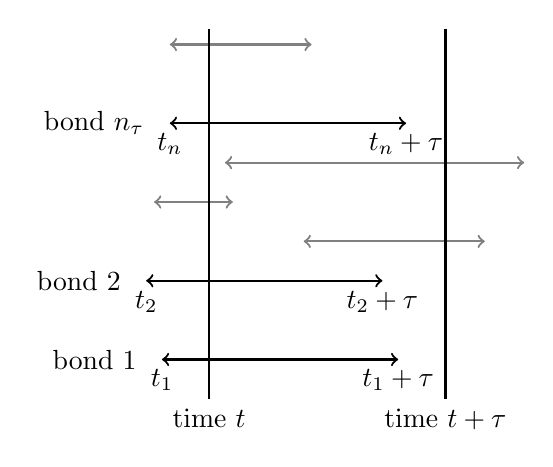
\begin{tikzpicture}[help lines/.style={thin,draw=black!50}]
%%\draw[help lines] (0,0) grid (4,4);
\draw [<->, thick] (0.4,0) node [anchor = north] {$t_1$} -- (3.4,0) node [anchor = north] {$t_1 + \tau$};
\draw (0.2,0) node [anchor = east] {bond $1$};
\draw [<->, thick] (0.2,1) node [anchor = north] {$t_2$} -- (3.2,1) node [anchor = north] {$t_2 + \tau$};
\draw (0,1) node [anchor = east] {bond $2$};
\draw [<->, thick] (0.5,3) node [anchor = north] {$t_n $} -- (3.5,3) node [anchor = north] {$t_n + \tau$};
\draw (0.3,3) node [anchor = east] {bond $n_{\tau}$};
\draw [gray,<->, thick] (1.2,2.5) -- (5.0,2.5);
\draw [gray,<->, thick] (0.3,2) -- (1.3,2);
\draw [gray,<->, thick] (2.2,1.5) -- (4.5,1.5);
\draw [gray,<->, thick] (0.5,4) -- (2.3,4) ;
\draw [thick] (1.0,4.2) -- (1.0,-0.5) node [anchor = north] {time $t$};
\draw [thick] (4.0,4.2) -- (4.0,-0.5) node [anchor = north] {time $t+\tau$};
\end{tikzpicture}
  \caption{\label{fig:P_tc} The H-bonds with lifetime $\tau$ in a certain configuration. 
At time $t$, we assume that there are totally $n_\text{tot}$ H-bonds can be detected, and $n_{\tau}$ H-bonds are of lifetime $\tau$, therefore,  the fraction of H-bonds that 
have the lifetime $\tau$ in the configuration at time $t$ is $P_\text{tc}(\tau) =  n_{\tau} /n_\text{tot}$.
Let $\tau$ take all the values in the interval $[0,\infty]$, we can get the HB lifetime distribution $P_\text{tc}(t)$.
}
\end{figure}

\paragraph{HB lifetime distributions}\label{diff_distr}
From the probability $P_\text{tc}(t)$ of the total HB lifetime in a configuration, and the probability $P_\text{a}$ of 
the first HB breaking in time $t$ after it have been detected at the moment $t$, one can introduce the average time 
$\langle \tau_\text{tc}\rangle$ and $\langle \tau_\text{a}\rangle$ :
\begin{equation}
\langle \tau_\text{tc}\rangle = \int_0^\infty t P_\text{tc}(t) dt,
\label{eq:tau_tc}
\end{equation}
\begin{equation}
\langle \tau_\text{a}\rangle = \int_0^\infty t P_\text{a}(t) dt. 
\label{eq:tau_a}
\end{equation}
Since $P_{\mathrm{a}}(t)=\int_{t}^{\infty} P_{\mathrm{tc}}(\tau) \frac{d \tau}{\tau}$, i.e., 
\begin{equation}
P_\text{tc}(t) = -t\frac{dP_\text{a}(t)}{dt}, \nonumber
\label{eq:relation_Ptc--Pa}
\end{equation}
integrating by parts, we obtain
\begin{eqnarray}
&&\langle \tau_\text{tc}\rangle = -\int_0^\infty t^2 \frac{dP_{\mathrm{a}}(t)}{dt}dt \nonumber \\
%
&&= -\int_0^\infty t^2 dP_\text{a}(t) \nonumber\\
&&= 2\langle \tau_\text{a}\rangle,\nonumber
\end{eqnarray}
in which we used $\int_0^\infty d(t^2 P_\text{a})=0$.

We denote the probability of the total HB lifetime along a trajectory as $P_{\mathrm{tt}}(t)$,
then the average HB lifetime over the trajectory is
\begin{eqnarray}
\left\langle\tau_{\mathrm{tt}}\right\rangle=\int_{0}^{\infty} t P_{\mathrm{tt}}(t) d t.
\label{eq:relation_tau_tt}
\end{eqnarray}
Because $\int_{0}^{\infty} P_{\mathrm{tc}}(t) d t=\frac{1}{\langle \tau_\text{tt}\rangle} \int_{0}^{\infty} t P_{\mathrm{tt}}(t) d t = 1$, 
we get 
\begin{eqnarray}
P_{\mathrm{tt}}(t)=\left\langle \tau_{\mathrm{tt}}\right\rangle P_{\mathrm{tc}}(t) / t.
\label{eq:relation_P_tt--P_tc}
\end{eqnarray}
The difference between the distribution functions, $P_{\mathrm{tt}}(t)$ and $P_{\mathrm{tc}}(t)$, can be described as follows.
$P_{\mathrm{tt}}(t)$ represents the percentage of pairs of molecules that had a continuous H-bonds during time $t$, 
while $P_{\mathrm{tc}}(t)$ the percentage of the number of H-bonds with a given lifetime $t$ 
to the number of all H-bonds in any configuration\cite{Voloshin2009}.

Since $P_{\mathrm{a}}(t)=\int_{t}^{\infty} P_{\mathrm{tc}}(\tau) \frac{d \tau}{\tau}$,
we can obtain
\begin{eqnarray}
&& P_{\mathrm{a}}(t)=\int_t^\infty \frac{P_\text{tt}}{\langle\tau_\text{tt}\rangle} \frac{\tau}{\tau} d\tau \nonumber \\
&& =  \int_t^\infty \frac{P_\text{tt}}{\langle\tau_\text{tt}\rangle}d\tau. \nonumber
\label{eq:P_a}
\end{eqnarray}
Let $t=0$, we have 
\begin{eqnarray}
P_{\mathrm{a}}(0)=1 /\left\langle t_{\mathrm{tt}}\right\rangle = 1 /\left\langle t_{\mathrm{HB}}\right\rangle.
\label{eq:P_a0}
\end{eqnarray}

From Eq. \ref{eq:tau_tc} and the relation between \SHB and $P_{\mathrm{a}}(t)$
\begin{eqnarray}
s(t)=\int_{t}^{\infty} P_{\mathrm{a}}(\tau) d \tau,
\label{eq:P_a}
\end{eqnarray}
we obtain
%
\begin{eqnarray}
&&\int_{0}^{\infty} \int_{t}^{\infty} P_\text{a}(t) d \tau d t = \int_{0}^{\infty} \int_{0}^{\tau} P_\text{a}(\tau) d t d \tau \nonumber \\
&& = \int_{0}^{\infty} \tau P_\text{a}(\tau) d \tau \nonumber \\
&& = \langle \tau_{\mathrm{a}} \rangle, \nonumber
\end{eqnarray}
i.e., 
\begin{eqnarray}
\int_{0}^{\infty} s(t) d t = \langle \tau_{\mathrm{a}} \rangle.
\label{eq:int_Ca}
\end{eqnarray}
\paragraph{Calculation of HB lifetime distributions}
In this paragraph, we describe the method to calculate the above lifetime distributions $P_\text{tc}(\tau)$, $P_\text{a}(\tau)$, and $P_\text{tt}(\tau)$.

First, we describe the method of calculating $P_\text{tc}(\tau)$.
Theoretically speaking, in order to calculate $P_\text{tc}(\tau)$, our detection time $t$ must meet the following conditions: 
$t-t_0 > \tau_\text{hb}^{\max}$, where $t_0$ is the initial time and $\tau_\text{hb}^{\max}$ is the maximum lifetime value of the H-bonds in the system. 
However, the value of $\tau_\text{hb}$ cannot be known in advance. 
In order to reduce the error, the method we can adopt is to set an empirical value as large as possible for
 $\tau_\text{hb}^{\max}$ if conditions permit. Since the value of $\tau_\text{hb}^{\max}$ is limited, in principle the lifetime value of the HB 
can always be greater than $\tau_\text{hb}^{\max}$. 
Therefore, the average value of the HB lifetime distribution 
calculated in this approximate way will move to a shorter lifetime than the average value of the true HB lifetime distribution:
\begin{eqnarray}
\int_{0}^{\infty} \tau P_{\mathrm{tc}}^{\mathrm{approx}}(\tau) d \tau < \left\langle\tau_{\mathrm{tc}}\right\rangle.
\label{eq:upper_bound_1_for_tau_tc}
\end{eqnarray} 

Among H-bonds detected at time $t$, if there are H-bonds that have existed at the beginning $t_0$ and 
remain in existence until time $t$, then we can approximately express the lifetime of these H-bonds as $\delta t^{(j)}=t^{(j)} -t_0$, 
where $j=1,\cdots, m$ is the labels of the $m$ H-bonds and $t^{(j)}$ is the moment when the $j$-th HB is broken. 
If we use $\tau^{(j)},j=1,\cdots,m$ to represent the true lifetimes of these $m$ H-bonds,
then we can find that $\tau^{(j)}-\delta t^{(j)} >0 $.
Since we cannot judge the true lifetime of these H-bonds, we can use $\delta t^{(j)}$ to approximate 
the lifetime of these $m$ H-bonds, that is
\begin{eqnarray}
\tau^{(j)} = \delta t^{(j)}, j=1,\cdots,m.
\end{eqnarray}
For those H-bonds that did not exist at the beginning, the method of calculating their lifetime is straightforward, 
the lifetime $\tau^{(j)}$ is equal to the time $t^{(j)}$ when the HB is broken minus the time $t^{{(j)}}_0$ of its formation:
\begin{eqnarray}
\tau^{(j)} = t^{(j)} - t^{(j)}_0,
\end{eqnarray} 
where the superscript $j = 1, \cdots, m'$, identifies $m'$ H-bonds 
detected at time $t$, and
formed after $t_0$ and broken at $t^{(j)}$.

Specifically, for DFTMD results, we approximate $P_\text{tc}$ as follows: 
We select evenly distributed $n$ time points $t=t_1,...,t_n$, from the trajectory obtained by the simulation, 
and count the HB lifetime at each time point $t_i$.
The distribution $P_\text{tc}(\tau)$ 
can be obtained by the average of the lifetime distribution detected at a certain time $t_i$, $i=1,\cdots, n$, 
where $t_i-t_{i-1} = \tau_\text{hb}^{\max}$. 

From the perspective of simulation data, we have another way to obtain $P_\text{tc}(\tau)$: 
Count the lifetimes of H-bonds that are formed after the initial time $t_0$ and are broken before the end time $t_\text{f}$.
%Although the distribution obtained in this method cannot be verified experimentally, it is the true distribution of HB bonds in simulated systems. 

\section{HB population operator}\label{hbpo}
\paragraph{Calculation of the reactive flux}\label{calc_rf}
For dynamical variables $x_i(t)$ and $x_k(t)$, their correlation functions have the following relationship\cite{Landau1980}:
\begin{equation}
\langle x_i(t') x_k(t)\rangle = -\langle x_i(t) x_k(t')\rangle.
\label{eq:correlation_relation}
\end{equation}
Let $x_i = h$, $x_k = \dot h$,
then, we obtain
\begin{equation}
\langle h(0) \dot{h}(t)\rangle=-\langle\dot{h}(0) h(t)\rangle. 
\label{eq:h_correl_relation}
\end{equation}
From the definition of the reactive flux $k(t) = -dc/dt$, we obtain 
\begin{equation}
k(t)=-\langle h(0) \dot{h}(t)\rangle /\langle h\rangle. 
\label{eq:rf1}
\end{equation}
Then from Eq. \ref{eq:h_correl_relation},
we get 
\begin{equation}
k(t) =  \langle \dot{h}(0)h(t)\rangle /\langle h\rangle. \nonumber
\label{eq:rf2}
\end{equation}
Since $\langle\dot{h}(0)\rangle=0$, $k(t)$ can be calculated by
\begin{equation}
k(t) = - \langle \dot{h}(0)[1-h(t)]\rangle /\langle h\rangle.
\label{eq:rf3}
\end{equation}


\paragraph{Relaxation time of H-bonds in bulk water}\label{rate_const_and_tau_R_128w}
% 
For the dynamic trajectory of such a system, we also calculated the self-correlation function $c(t)$ of the HB population operator, 
and the functions $k(t)$ and $n(t)$ derived from it. 
Tables \ref{tab:k_k_prime_128w_1} and \ref{tab:k_k_prime_128w_2} show the rate constants $k$ and $k'$, and 
the relaxation time $\tau_\text{HB}$ obtained by the least squares fit method. 
%It can be seen from the tables that the accuracy of the calculation of $k$, $k'$ are accurate to at least two decimal places.

%
\begin{table}[H] %[htbp]
\centering
\caption{\label{tab:k_k_prime_128w_1} 
    The $k$ and $k'$ for bulk water. We carried on the short time region 0.2 ps $< t <$ 2 ps. 
The unit for $k$ ($k'$) is ps$^{-1}$, and that for $\tau_{\text{HB}}$ ($=1/k$) is ps. The $h(t)$ is bond-based.} 
\begin{tabular}{cccc}
 Criterion & $k$  (bulk) & $k'$ (bulk) & $\tau_{\text{HB}}$ (bulk) \\
\hline
  %ADH & 0.335 & 0.937 & 2.988  \\
  %ADH(from $k_{in}$) & 0.299  & 1.029 & 3.347   \\
  %AHD & 0.322 & 1.01 & 3.101 \\ 
  %AHD(from $k_{in}$) & 0.288 & 1.121 & 3.468 \\ 
  ADH & 0.299  & 1.029 & 3.347   \\
  AHD & 0.288 & 1.121 & 3.468 \\ 
\end{tabular}
\end{table}
%
\begin{table}[H]%[htbp]
\centering
\caption{\label{tab:k_k_prime_128w_2} 
    The $k$ and $k'$ for bulk water. We carried on the long time region 2 ps $< t <$ 12 ps. 
The unit for $k$ ($k'$) is ps$^{-1}$, and that for $\tau_{\text{HB}}$ ($=1/k$) is ps. The $h(t)$ is bond-based.} 
\begin{tabular}{cccc}
 Criterion & $k$  (bulk) & $k'$ (bulk) & $\tau_{\text{HB}}$ (bulk) \\
\hline
  %ADH & 0.103 & 0.024 & 9.690 \\
  %ADH(from $k_{in}$) & 0.103  & 0.028 & 9.728 \\
  %AHD & 0.104 & 0.034 & 9.656  \\
  %AHD(from $k_{in}$) & 0.103  & 0.040 & 9.702  \\
  ADH & 0.103  & 0.028 & 9.728 \\
  AHD & 0.103  & 0.040 & 9.702  \\
\end{tabular}
\end{table}

%\paragraph{Different definitions of the $h(t)$}\label{DEF_POPULATION_OPERATOR}
%Here we discuss the definition of another possible hydrogen bond population operator $\tilde{h}(t)$ besides $h(t)$ introduced in the text.
%When a pair of water molecules $a$ and $b$ are H-bonded, 
%the oxygen atom in each water molecule can act both as a donor and an acceptor. 
%In particular, a pair of water molecules can form 4 different forms of H-bonds. 
%In other words, if the role of H atoms between the pair of water molecules changes, but they still form H-bonds, 
%we think that an old H-bond is broken and a new H-bond is formed.

%The correlation functions \CHB of water molecules in bulk water is shown in Fig. \ref{fig:bk_water_c_two_population_operators_with_ADH}.
%It shows that there are big differences in the correlation functions of the two definitions $h(t)$ and $\tilde{h}(t)$,
%because hydrogen exchange is considered in the O--H pair-based HB population $\tilde{h}(t)$, but not in the W--W pair-based HB population $h(t)$.
% bk_water_c_two_population_operators_with_ADH.eps
% /home/gang/Github/water_pair_HB_dynamics/plot/plot_c/bk_water_c_two_population_operators_with_ADH.eps
% old version: 128w_bk--water-pair-based_and_bond-based_c.eps
%\begin{figure} [htbp]
%\centering
%	\includegraphics [width=0.36\textwidth] {./diagrams/bk_water_c_two_population_operators_with_ADH}
%\setlength{\abovecaptionskip}{0pt}
%	\caption{\label{fig:bk_water_c_two_population_operators_with_ADH} The correlation functions \CHB of water molecules in bulk water (ADH criterion). 
%        Here HB population is based on two different definitions, one is based on a pair of water molecules (solid line),\cite{Khaliullin2013} 
%and the other is based on O--H pairs between water molecules (dashed line).}
%\end{figure} 

%\section{Fitting $C_2(t)$ with a single exponential function}\label{single_exp}
%We assume that the anisotropy decay $C_2(t)$ is a single exponential given by 
%\begin{equation}
%C_2(t) = A e^{-\kappa t},
%\label{eq:tcf2}
%\end{equation}
%where $\kappa$ is a relaxation rate constant of the anisotropy decay. For each value of $\kappa$, we denote the relaxation period as $1/\kappa$.
%The $C_2(t)$ for water molecules in different environments in LiI solution at 330 K is shown in
%Fig.\thinspace\ref{fig:2LiI-124w_c2_fit_5_single-exp}.
%\begin{figure} [htbp]
%\centering
%	\includegraphics [width=0.60\textwidth] {./diagrams/2LiI-124w_c2_fit_5_single-exp}
%\setlength{\abovecaptionskip}{0pt}
%	\caption{\label{fig:2LiI-124w_c2_fit_5_single-exp} The anisotropy decay of OH bonds in water molecules at the interface of LiI solutions.}
%\end{figure} 
%It is evident, from the figure, that $C_2(t)$ for water molecules neither in the bulk or at interface of the LiI solution can \emph{not} be described as a single exponential dynamics.  Besides, we also have fitted the $C_2(t)$ for water molecules in NaI solution and the result is the same as above. The fitting parameters for LiI and NaI solution are presented in table \ref{tab:c2_single-exp-fitting_LiI} and \ref{tab:c2_single-exp-fitting_NaI}, respectively.
%%-- 
%\begin{table}
%\centering
%\caption{\label{tab:c2_single-exp-fitting_LiI}%
%	The single-exponentially fitted parameters---the amplitude $A$, the decay rate $\kappa$, the relaxation period $1/\kappa$, of anisotropy decay for water molecules 
%  at the interface of 0.9 M LiI solutions, at 330 K.} 
%\begin{tabular}{lccc}
%	water molecules &  $A$ & $\kappa$ (THz) & $1/\kappa$ (ps)  \\
%\hline
%	I$^-$-shell  & 0.83  & 0.26  & 3.85  \\
%	Li$^+$-shell & 0.89  & 0.07  & 14.29 \\
%	bulk & 0.86 & 0.12 & 8.33 \\
%	surface & 0.75 & 0.29 & 3.45 \\
%\end{tabular}
%\end{table}
%%-- 
%\begin{table}[H]
%\centering
%\caption{\label{tab:c2_single-exp-fitting_NaI}%
%	The single-exponentially fitted parameters---the amplitude $A$, the decay rate $\kappa$, the relaxation period $1/\kappa$, of anisotropy decay for water molecules 
%	at the interface of 0.9 M NaI solutions, at 330 K.} 
%\begin{tabular}{lccc}
%	water molecules &  $A$ & $\kappa$ (THz) & $1/\kappa$ (ps)  \\
%\hline
%	I$^-$-shell  & 0.86  & 0.14  & 7.14 \\
%	Na$^+$-shell & 0.79 & 0.07  & 14.29 \\
%	bulk & 0.83 & 0.06  & 16.67 \\
%	surface & 0.78 & 0.12 & 8.34 \\
%\end{tabular}
%\end{table}

%\section{Reorientation dynamics of water molecules at solution/vapor interfaces}\label{C2_DOUBLE_FIT}
%\paragraph{Double exponential fit}
%In general, the rotational motion of water molecules are not simply characterized by a well-defined rate constant. 
%Similar non-single-exponential kinetics is also obtained in HB dynamics 
%in liquid water\cite{AL96,Dirama2005} and in the time variation of the average frequency shifts of the 
%remaining modes after excitation in hole burning technique\cite{Rey2002,Moller2004}.
%We can understand the non-single-exponential kinetics of rotational 
%anisotropy decay by fitting the rotational anisotropy decay by a 
%biexponential function.

%To obtain the effects of diffusion and HB decay of water molecules
%in solutions respectively, we assume that 
%the correlation function $C_2(t)$ has the form\cite{TanHS2005}
%\begin{equation}
%C_2(t)=A_1e^{-t/\tau_{2,1}} +A_2e^{-t/\tau_{2,2}},
%\label{eq:tcf3}
%\end{equation}
%where $A_i$ are amplitudes and $1/\tau_{2,i}$ ($i=1, 2$) are decay rates of $C_2(t)$,
%and the $\tau_{2,i}$ represent the relaxation times of the $C_2(t)$. 
%%(DONE: Here I should comment on which is the physical meaning of a double exponential.)
%Here, we assume that the orientation relaxation $C_2(t)$ is composed of two independent relaxation processes 
%with different time scales, and each process can be described by an exponential decay function, respectively.
%For alkali-iodine solutions (LiI and NaI), the $A_i$ and $\tau_{2,i}$ of the biexponentials fits for functions 
%$C_2(t)$ are shown in Table ~\ref{tab:table8}.
%%As an example, for the interface of LiI solution, we made a comparison between $C_2(t)$ 
%%and the function fitted according to Eq.\thinspace\ref{eq:tcf3},
%%as shown in Fig.\thinspace\ref{fig:2LiI-124w_c2_fit_5ps_biexp}. 
%We found that Eq. \ref{eq:tcf3}, the biexponential kinetics is sufficiently accurate to 
%describe the characteristics of anisotropy decay.                        

%Then we considered the effect of ion species in solution/vapor interfaces on the anisotropy decay of water molecules.
%%(DONE: Here is on the surface or not? interfaces.).
%For both LiI and NaI solutions, there are two decay processes 
%(Table \ref{tab:table8})
%--- amplitude $\sim 1$,
%decay time $\tau_{2,2}\sim$ 10.0 ps, and for the other describe the initial fast decay 
%of the anisotropy, with amplitude $\sim 0.1$, decay time $\tau_{2,1}\sim$ 0.1--1.0 ps, 
%due to the inertial--librational motion preceding the orientational diffusion.
%%The one describe the initial fast decay of the anisotropy, 
%%with amplitude $\sim$ 0.1, decay constant $\sim$ (1--10) THz,
%%results from the inertial-librational motion preceding the orientational diffusion.
%%


%%{Fitting by a biexponential}
%\begin{table}[H]  % or [!htbp]
%\centering
%\caption{\label{tab:table8}
%The fitted parameters of anisotropy decay of water molecules at the LiI (NaI, KI) solution/vapor interface 
%according to Eq. \ref{eq:tcf3} for the time range [0,10] ps. The standard errors: $\delta A_i \sim 0.01$, $\delta \tau_{2,i} \sim 0.1$ ps ($i=1,2$).}
%\begin{tabular}{lccccc}
%\wat & $A_1$  & $\tau_{2,1}$ (ps) & $A_2$ & $\tau_{2,2}$ (ps) \\
%\hline
%%\I-shell (LiI)  &0.45 & 3.23  & 0.45 & 3.23\\
%\Li-shell & 0.56 & 8.3 & 0.33 & 50.0  \\
%%bulk (LiI) &0.43  & 9.09 & 0.43 & 8.33 \\
%%surface (LiI) & 0.41 & 2.86 & 0.40  & 2.78 \\
%\I-shell &0.86 & 7.1 & 0.08 & 0.1 \\
%\Na-shell & 0.71 & 16.7 & 0.19 & 1.3 \\
%%Bulk water & 0.60 & 13.51 & 0.31  & 3.45 \\
%%bulk (NaI) & 0.81 & 16.67 & 0.099  & 0.80  \\
%LiI/vapor & 0.84 & 4.9 & 0.09 & 0.6 \\ 
%NaI/vapor & 0.77 & 9.1 & 0.13 & 0.4 \\
%KI/vapor & 0.80 & 6.1 & 0.12 & 1.1 \\
%\end{tabular}
%\label{tab:biexponential1}
%\end{table}
%%{Fitting by a single exponential}
%The orientation relaxation time constants $\tau_{2,i}$ and amplitudes $A_i$ ($i=1,2$) of the single exponential fits (10 ps) for $C_2(t)$ are in Table \ref{tab:table8}.
%For comparison, we also fit $C_2(t)$ for water molecules at each interface with a single exponential (Table \ref{tab:1exp_alkali-iodide}). 
%It can be seen that the value of $\tau_2$ is between the two characteristic times $\tau_{2,1}$ and $\tau_{2,2}$, obtained by biexponential fitting. 
%At the same time, we can see the obvious difference in water molecules under various conditions: 
%the reorientation characteristic time $\tau_2$ in the first solvation shell of alkali metal ions is 2 to 3 times that of I$^-$ ion.
%This is a reasonable result. However, the single exponential model describes the reorientation of water molecules 
%as an exponential decay process. The above biexponential function model (Eq. \ref{eq:tcf3}) can be explained as: 
%the reorientation dynamics of each water molecule is composed of two independent decay processes.
%One has amplitude $\sim$ 1, decay time $\sim$ 10 ps, which describes the initial fast decay of the anisotropy, 
%and the other is of amplitude $\sim$ 0.1, decay time $\sim$ 0.1 ps, due to the inertial-librational motion preceding the orientational diffusion.
%\begin{table}[H]  % or [!htbp]
%\centering
%\caption{\label{tab:1exp_alkali-iodide}
%The fitted (single exponential) parameters of anisotropy decay of water molecules at the LiI (NaI, KI) solution/vapor interface 
%according to Eq. \ref{eq:tcf3} for the time range [0,10] ps. The standard errors: $\delta A \sim 0.01$, $\delta \tau_{2} \sim 0.1$ ps.}
%\begin{tabular}{lccccc}
%\wat & $A$  & $\tau_{2}$ (ps) \\
%\hline
%\Li-shell & 0.88 & 13.7 \\
%\I-shell & 0.83 & 3.9 \\
%\Na-shell & 0.84 & 10.1 \\
%LiI/vapor & 0.80 & 3.0 \\ 
%NaI/vapor & 0.86 & 4.2 \\ %scr_c2--121_pure--2KI_2NaI_16--inset_fit_single-exp.gp
%KI/vapor & 0.86 & 5.7 \\ %scr_c2--121_pure--2KI_2LiI_16--inset_fit_single-exp.gp
%\end{tabular}
%\label{tab:biexponential1}
%\end{table}

\chapter{Structural characterization of water clusters and solutions}
\section{Water clusters}\label{structure_of_clusters}
The structural parameters of the considered water clusters are shown here.
Table \ref{tab:3_nitrate_bond_0} gives the average HB lengths $r_a$ (with standard deviations) in [NO$_3\cdot$(H$_2$O)$_3$]$^-$.  
Table \ref{tab:3w_nitrate} (\ref{tab:table_geo_opt}) reports the selected distances characterizing 
[NO$_3\cdot$(H$_2$O)$_3$]$^-$ (RNO$_3$(H$_2$O)$_3$), and Table \ref{tab:table_rnitrate_3w} the selected parameters for RNO$_3$   
 (H$_2$O)$_3$ (R=Li, Na, K).
The unit for length and angle are \AA and degree ($^\circ$), respectively.
% 
\begin{table}[!h]
\centering
\caption{\label{tab:3_nitrate_bond_0}%
HB lengths $r_a$ in [NO$_3\cdot$(H$_2$O)$_3$]$^-$.} % T=300 K. 
\begin{tabular}{cc} \\\toprule
 HB bound to & \multicolumn{1}{c}{ $r_a$} \\
\hline
 w1 &2.40$\pm$0.52; 3.02$\pm$0.72 \\
 w2 &2.56$\pm$0.48; 3.20$\pm$0.41 \\
 w3 &2.29$\pm$0.47; 3.11$\pm$0.72
\end{tabular}
\end{table}
%
\begin{table}[!htbp]
\centering
\caption{\label{tab:3w_nitrate}%
Parameters of water molecules and H-bonds in [NO$_3\cdot$(H$_2$O)$_3$]$^-$.} % T=300 K.
\begin{tabular}{lccc}
water &$R_\text{OH}$ &$\angle$HOH & $r_\text{OH}$ \\
\hline
w1 &0.98$\pm$0.02 &101$\pm$4 & 2.40$\pm$0.52, 3.02$\pm$0.72 \\
w2 &0.98$\pm$0.02 &101$\pm$5 & 2.56$\pm$0.48, 3.20$\pm$0.41 \\
w3 &0.98$\pm$0.02 &101$\pm$4 & 2.29$\pm$0.47, 3.11$\pm$0.72
\end{tabular}
\end{table}
%
\begin{table}[!htbp]
\centering
\caption{\label{tab:table_geo_opt}%
  Structural parameters of RNO$_3$(H$_2$O)$_3$ from geometry optimization.} 
\begin{tabular}{l*{4}ccc}
Parameter  & LiNO$_3$(H$_2$O)$_3$& NaNO$_3$(H$_2$O)$_3$ & KNO$_3$(H$_2$O)$_3$\\
\hline
$r_\text{HB1}$& 1.67 & 1.71 & 1.82 \\
$r_\text{HB2}$& 1.91 & 1.78 & 1.92\\
$r_\text{HB3}$& 1.82 & 1.69 & 1.94\\
$r_\text{R-O(w1)}$ & 1.91 & 2.31 & 2.70\\
$r_\text{R-O(w2)}$ & 1.90 & 2.26 & 2.70\\
$r_\text{R-O(\nitrate)}$ & 1.84 & 2.29 & 2.69 \\
$\angle$HOH(w1)& 109 & 106 &107 \\
$\angle$HOH(w2)& 106 & 105&105 \\
$\angle$HOH(w3)& 108 & 107 &106
\end{tabular}
\end{table}
%
\begin{table}[H] %[!htbp]
\centering
\caption{\label{tab:table_rnitrate_3w}%
Parameters of RNO$_3$(H$_2$O)$_3$ at 300 K, obtained from the averaging during a DFTMD trajectory. 
  For RNO$_3$(H$_2$O)$_3$, $R_\text{OH}$ and $R'_\text{OH}$ 
  denote the lengths of O-H bonds in which H atoms is H-bonded and is free, respectively.
  }
\begin{tabular}{l*{4}lll}
Parameter & LiNO$_3$(H$_2$O)$_3$& NaNO$_3$(H$_2$O)$_3$ & KNO$_3$(H$_2$O)$_3$\\
\hline
$r_\text{HB1}$ & $1.83\pm0.14$ & $1.78\pm0.09$ & $1.82\pm0.13$\\
$r_\text{HB2}$ & $2.00\pm0.25$ & $1.91\pm0.24$ & $1.80\pm0.12$\\
$r_\text{HB3}$ &$1.79\pm0.16$ & $1.76\pm0.11$ & $1.89\pm0.18$\\
$R_\text{OH}$(w1) &$0.97\pm0.01$ &$0.98\pm0.04$ &$0.97\pm0.03$ \\
$R'_\text{OH}$(w1) &$1.00\pm0.02$ &$1.00\pm0.02$ & $1.00\pm0.03$ \\
$R_\text{OH} $(w2) &$0.97\pm0.01$ &$0.98\pm0.02$ &$0.97\pm0.02$ \\ 
$R'_\text{OH}$(w2) &$0.99\pm0.01$ &$1.00\pm0.02$ & $1.00\pm0.03$ \\
$R_\text{OH}$(w3) &$0.97\pm0.01$ & $0.97\pm0.02$&$0.97\pm0.03$ \\
$R'_\text{OH}$(w3) &$1.00\pm0.02$ &$1.00\pm0.02$ & $1.00\pm0.03$ \\
$r_\text{R-O(w1)}$ & $1.95\pm0.09$ & $2.34\pm0.08$ & $2.76\pm0.11$\\
$r_\text{R-O(w3)}$ & $1.92\pm0.07$ & $2.32\pm0.11$ & $2.74\pm0.13$\\
$r_\text{R-O(\nitrate)}$ & $1.91\pm0.08$ & $2.31\pm0.09$ & $2.74\pm0.12$ \\
$\angle$HOH (w1) &$107\pm4$ & $106\pm4$ &$105\pm5$ \\
$\angle$HOH (w2) &$106\pm6$ & $105\pm4$ &$106\pm4$ \\
$\angle$HOH (w3) &$108\pm5$ & $106\pm3$ &$106\pm3$ 
\end{tabular}
\end{table}
\paragraph{Structural and vibrational properties of [NO$_3\cdot$(H$_2$O)$_3$]$^-$}
% [In the main text, I deleted this paragraph, because now i am not sure on this idea.]
To find possible source of the vibrational features of water molecules in the 
cluster [NO$_3\cdot$(H$_2$O)$_3$]$^-$, we consider structural properties and the VDOS for water molecules 
in it. 
Lengths of H-bonds are shown in Table\thinspace\ref{tab:3_nitrate_bond}. 
The nitrate O (ON)--water O (OW) 
and nitrate O--water H (HW) RDFs are shown in Fig.\thinspace\ref{gdr_ON-wat--3_NO3}.

%
When $T=300$ K, the difference $r_a$ between different H atoms in one water molecule is
$\Delta{r_a}=0.69$ \AA, while $\Delta{r_a}=0.13$ \AA for $T=100$ K. It shows that vibrational 
peaks for the three water molecules are much closer than that at the higher temperature 300 K. 

%
The calculated VDOS for water molecules in the cluster at a lower temperature 100 K is given in 
Fig.\thinspace\ref{fig:vdos_LiNO3-3w_100K_w1-2-3_font35}. 
It shows that the vibrational peaks for the three water molecules 
are close to each other ($\Delta\nu <$ 10 \cm) for both vibrational and bending modes.
At the lower temperature, the three water molecules 
are more symmetric distributed bound to the central nitrate. Therefore, the difference between H-bonds in the 
symmetric isomer of [NO$_3\cdot$(H$_2$O)$_3$]$^-$ is likely a finite temperature effect,
which can be verified by the calculation of the VDOS for water molecules.

%
Both differences $\Delta\nu$ and $\Delta{d}$ decrease as the temperature decrease,
therefore, the different vibrational features are $T$-dependent effect. 

\begin{table}[H]
\centering
\caption{\label{tab:3_nitrate_bond}%
Lengths of H-bonds in [NO$_3\cdot$(H$_2$O)$_3$]$^-$. Indices of H atoms: H6, H7 in w1; 
H9, H10 in w2; and H12, H13 in w3.} 
\begin{tabular}{ccc} \\\toprule
 HB & $r_a\pm\delta$ (100 K)(\A) & \multicolumn{1}{c}{ $r_a\pm\delta$ (300 K)}(\A)\\
\hline
 H6-O2 &2.75$\pm$0.62& 2.40$\pm$0.52 \\
 H7-O4 &2.79$\pm$0.58& 3.02$\pm$0.72 \\
 H9-O3 &2.89$\pm$0.60 &2.56$\pm$0.48 \\
 H10-O4 &2.74$\pm$0.49&3.20$\pm$0.41 \\
 H12-O3 &2.46$\pm$0.45&2.29$\pm$0.47 \\
 H13-O2 &2.75$\pm$0.59 &3.11$\pm$0.72
\end{tabular}
\end{table}
%===================
\begin{figure}[H] %[htbp]
\centering
\includegraphics [width=0.5\textwidth] {./diagrams/gdr_ON-wat--3_NO3} 
\setlength{\abovecaptionskip}{0pt}
\caption{\label{gdr_ON-wat--3_NO3}
The nitrate O (ON)--water O (OW) 
and nitrate O--water H (HW) RDFs for [NO$_3\cdot$(H$_2$O)$_3$]$^-$.
Peaks for the former are 1.93, 2.95 and 3.95 \A, and for the later are 2.95 and 4.80 \A.}
\end{figure} 
%==================================================================================
%--------------------
\begin{figure}[H]%[htbp]
\centering
\centering
\includegraphics [width=0.5 \textwidth] {./diagrams/vdos_LiNO3-3w_100K_w1-2-3_font35} 
\setlength{\abovecaptionskip}{0pt}
\caption{\label{fig:vdos_LiNO3-3w_100K_w1-2-3_font35} The VDOS $g(\nu)$ for water molecules in the
cluster [NO$_3\cdot$(H$_2$O)$_3$]$^-$ at 100 K.} 
\end{figure}
%====================================================================================
%In addition, the VDOS for H atoms and water molecules in [NO$_3\cdot$(H$_2$O)$_3$]$^-$ (Fig.\thinspace\ref{fig:vdos_NO3-3w_2_H-wat}) shows 
%that H's contribution dominates that of the water molecule. 

\section{Solution/vapor interfaces}\label{SOLUTION_VAPOR_PROPERTIES}
%\paragraph{Dipole orientation distribution of water at aqueous/vapor interfaces}
%Set $\theta$ as the angle between the dipole moment of water molecules and the normal vector 
%of the interface, and $P(\theta)$ as the probability.
%The data used to statistics is the dipole tilt angle $\theta_{i}$. 
%We use the $\theta_i$ instead of $\langle\theta\rangle$ to do the statistics.
%With picking up $\theta_{l}$, $l=0, 10, 20, ...$ from the series $\theta_{i}$,
%we find that pure water's dipole moment tilt angle is smaller than that of water molecules at the salty water surface. 
%This result means that at the pure water surface, water molecules have more $p$-polarization components than those at the salty water surface. 
%However, water molecules at the salty water surface has more $s$-polarization component.
%The result is shown in Fig.\thinspace\ref{fig:prob_theta_ln_itp_256}.
%%
\paragraph{Solvation shell HB dynamics of W--W bonds at the alkali iodide/vapor interfaces}
%%%%%%%%%%%%
% !?USEFUL %
%%%%%%%%%%%%
%%
%[ALSO INTERESTING TO COMPARE THESE CURVES TO THOSE FOR THE NEAT WATER/VAPOR INTERFACE] 
\begin{figure}[H]
\centering
\includegraphics [width=\textwidth] {./diagrams/hbacf_C_sh2_2p}
\setlength{\abovecaptionskip}{0pt}
\caption{\label{fig:hbacf_C_sh2_2p}The $c^{(k)}(t)$ of W--W bonds in the solvation shell 
  of (a) cations and (b) I$^-$ at the interfaces of 0.9 M LiI, NaI and KI solutions, respectively.
  As a reference, the \CHB for the 1-\AA water/vapor interface (Paragraph\thinspace\ref{PARA_IHB} in Chapter \ref{CHAPTER_HBD}) and bulk water are also shown.
%The data for bulk water are calculated from water in the middle of the slab of the LiI solution.
}
\end{figure}
%Fecko and co-workers' study of liquid D$_2$O by IR spectroscopy reveals that the vibrational dynamics observed are dominated by underdamped displacement of the hydrogen-bond coordinate at short times ( less than 200 fs).\cite{CJF03,CJF05} 

Figures \thinspace\ref{fig:hbacf_C_sh2_2p} a and b 
report the  $c^{(k)}(t)$ of W--W bonds in the solvation shell of cations and I$^-$ at the interfaces of the alkali iodide solutions.
%[HOW TO EXPLAIN (a)?] [(WHAT DOES THIS SENTANCE FOR?)
The interface of the LiI solution contains H-bonds between water molecules similar to those in bulk water, i.e.,
water molecules participating in these H-bonds are not in the solvation shell of ions. 
This result is consistent with the observation of femtosecond mid-infrared pump-probe experiments 
on the O--H stretch vibration of water molecules in aqueous solution,
that changing the nature of the cation does not affect the dynamics of solvating water\cite{Kropman2001}.
It is also in agreement with to the following \abinitio simulation results: water molecules that directly surround the cation, the O--H groups point
away from the cation and form O--H$\cdots$O bonds with bulk water molecules\cite{Hashimoto1994,Ramaniah1998,Kropman2001}.
From Fig.\thinspace\ref{fig:hbacf_C_sh2_2p} b, we found that for all three alkali iodide solutions, $c^{(k)}(t)$ for solvation shell  
of \I decays faster than that for molecules in bulk water.
The simulation produces similar result as Omta and coworker's experiments of femtosecond pump-probe spectroscopy,
which demonstrate that anions ( $\text{SO}^{2-}_4$, $\text{ClO}^-_4$, etc) have no influence on the dynamics of bulk water, 
even at high concentration up to 6 M\cite{Omta2003, ZhangYanjie2006}. 
Here, we have found that the cations \Li and \Na do not alter the H-bonding network outside the first solvation shell of cations. 
It is concluded that no long-range structural-changing effects for alkali metal cations.

In addition, \CHB for the instantaneous interface layer of thickness $d=1$ \AA in pure water is also shown in Fig.\thinspace\ref{fig:hbacf_C_sh2_2p}.
Its ultrafast relaxation process has a shorter relaxation time, which shows that the effects of ions (alkali cations and \I) are not as obvious as that of the water/vapor interface.


\paragraph{RDFs in alkali nitrate solutions}
%\{figure}[htb]
%\centering                                          
%\includegraphics [width=0.36 \textwidth] {./diagrams/gdr_N-W_127_LiNO3} 
%\setlength{\abovecaptionskip}{0pt}
%  \caption{\label{fig:gdr_N-W_127_LiNO3} RDFs $g_{N-OW}(r)$ and $g_{N-HW}(r)$ in bulk LiNO$_3$ solution.
%Box size: 15.78 $\times$ 15.78 $\times$ 15.78 \A$^3$; $T = 300$ K.}
%\end{figure}
RDFs $g_\text{Li-OW}(r)$, $g_\text{Li-HW}(r)$, $g_\text{ON-OW}(r)$ and $g_\text{ON-HW}(r)$ in bulk LiNO$_3$ solution are shown in Fig.\thinspace\ref{fig:gdr_127_LiNO3}.
\begin{figure}[H] %[htb]
\centering                                          
\includegraphics [width=0.8 \textwidth] {./diagrams/gdr_127_LiNO3} 
\setlength{\abovecaptionskip}{0pt}
  \caption{\label{fig:gdr_127_LiNO3} RDFs $g_\text{Li-OW}(r)$, $g_\text{Li-HW}(r)$, $g_\text{ON-OW}(r)$ and $g_\text{ON-HW}(r)$ in bulk LiNO$_3$ solution.}
%Box size: 15.78 $\times$ 15.78 $\times$ 15.78 \A$^3$; $T = 300$ K.
\end{figure}
%
\paragraph{RDFs in alkali iodide solutions}
RDFs $g_\text{Li-OW}(r)$, $g_\text{Li-HW}(r)$, $g_\text{I-OW}(r)$ and $g_\text{I-HW}(r)$ for the LiI/vapor interface are shown in Fig.\thinspace\ref{fig:gdr_124_2LiI}.
\begin{figure}[H]%[htb]
\centering                                          
\includegraphics [width=0.8 \textwidth] {./diagrams/gdr_124_2LiI} 
\setlength{\abovecaptionskip}{0pt}
  \caption{\label{fig:gdr_124_2LiI} RDFs $g_\text{Li-OW}(r)$, $g_\text{Li-HW}(r)$, $g_\text{I-OW}(r)$ and $g_\text{I-HW}(r)$ for the LiI/vapor interface.}
%Box size: 15.60 $\times$ 15.60 $\times$ 31.00 \A$^3$; $T = 330$ K.
\end{figure}
The radii of the second solvation shell are: 5.0 \AA for \li, 5.38 \AA for \na,
and 6.0 \AA for \I ions, which are obtained from the RDFs.
The RDFs $g_{\text{X-O}}$ (X=\li, \na, K$^+$) for the interfaces 
of LiI (NaI,KI) solutions are shown in Fig.\thinspace\ref{fig:gdr_XO--124_2XI} a,
and the coordination numbers are in Fig.\thinspace\ref{fig:gdr_XO--124_2XI} b.
We see that the radius of the solvation shells of \Li ions, \Na ions, 
and \K ions increase sequentially, and the number of coordination molecules also increase sequentially. 
However, this order is not true for the relaxation time of HB dynamics between water molecules in the first solvation shell of the ion 
and other water molecules. 
The effects of the alkali metal ions and iodide ions are similar
(Fig.\thinspace\ref{fig:hbacf_C_sh2_2p}), 
that is, the relaxation time of HB dynamics in the outer layer is smaller than that in bulk water.
%从图中我们看出,锂离子,钠离子,钾离子的溶解壳的半径依次增大,其配位分子数也依次增大。但这种有序性对于离子第一溶解壳内的水分子与其他水分子之间的氢键的弛豫时间却不成立。因为从7.5图可以看出,R离子和碘离子的效应很类似,即,其外层的HBD的弛豫时间都比体相纯水中的更小。
%为了看清不同溶液中的氢键的差别,我们在下一段研究了I-H氢键的动力学.
\begin{figure}[H]
\centering
\includegraphics [width=0.6\textwidth]{./diagrams/gdr_XO--124_2XI}%fig.6.1 
\setlength{\abovecaptionskip}{0pt}
\caption{\label{fig:gdr_XO--124_2XI}
(a) RDFs $g_{\text{X-O}}(r)$(X=\li, \na, K$^+$) and (b) the coordination number of \Li (\na, K$^+$) ions at the interfaces of LiI (NaI, KI) solution. 
The coordination numbers are $n_{\text{Li}^+}$=4, $n_{\text{Na}^+}$=5 and $n_{\text{K}^+}$=6.} 
\end{figure} % There is a first shell exist for both \Li and \Na cations. %(NEED the NORMED VERSION)
%%
%\begin{table}[H] %[!hbtp]
%\centering
%\caption{\label{tab:table_CoordNo}%
%The coordination number for ions in LiI (NaI) solution.}
%\begin{tabular}{lccc}
%name & $r_\text{shell}$ (\AA) & coordination number \\
%\hline
%$n_\text{Li-O}$ & 3.0 & 4.0 \\
%$n_\text{I-H}$ & 3.3 & 5.5 \\
%$n_\text{Na-O}$ & 3.5 & 6.0 \\ 
%$n_\text{I-O}$ & 4.3 & 5.8 \\
%\end{tabular}
%\end{table}
%\FloatBarrier
\section{Free energy of the water separated and the contact ion pair}\label{calculate_free_energy} 
From the blue-moon ensemble method\cite{Carter1989,Sprik1998}, we have obtained the constraint force (unit: a.u.force) acting on the atoms. 
The distance between the ion pair (unit: \A) is chosen as the reaction coordinate, the formula for calculating the free energy (unit: kcal/mol) is given as follows.
%First, note that
%\begin{equation}
%  1\ \text{a.u.force} =8.2387\times 10^{-8}\ \text{N}\nonumber;
%\label{eq:au2n}
%\end{equation}
%\begin{equation}
%  1\ \text{\A} = 10^{-10}\ \text{m} \nonumber;
%\label{eq:aa}
%\end{equation}
%\begin{equation}
%  1\ \text{J} = 1.44\times 10^{20}\ \text{ kcal/mol}.\nonumber
%\label{eq:j2kcpm}
%\end{equation}
The relative free energy is given by
%\begin{equation}
%  F = \sum_{i}^{N}f_i{\Delta{r}} \ \text{ a.u.energy},
%  \label{eq:f-e}
%\end{equation}
\begin{equation}
  F = \sum_{i}^{N}f_i{\Delta{r}},\nonumber
  \label{eq:f-e}
\end{equation}
where $i$ denote a point on the one-dimensional reaction coordinate, 
$N$ is the number of the sampling points of the reaction coordinates,
and $f_i$ denotes the average force on atoms over the trajectory when $i$ is fixed. 
%Furthermore,
%\begin{equation}
%  \begin{split}
%  &F = \sum_{i}^{N}f_i{\Delta{r}}\times 8.2387\times10^{-18}\text{ J}\\
%  &= \sum_{i}^{N}f_i{\Delta{r}}\times 8.2387\times10^{-18}\times1.44\times10^{20}\text{ kcal/mol}.
%  \end{split}
%\label{eq:f-e2}
%\end{equation}
Now we estimate the error of the free energy $\delta{F}$ from the summation approximation. It reads
\begin{equation}
  \delta{F} = \frac{1}{N}\sum_{i}^{N}\delta{f_i}{\Delta{r}}.
  \label{eq:dleta_f}
\end{equation}
Usually, $\delta{f_i}\approx\delta{f}$, thus
\begin{equation}
  \delta{F} = \frac{1}{N}\delta{f}\sum_{i}^{N}{\Delta{r}}.
\label{eq:dleta_f-2}
\end{equation}
Particularly, if $\Delta{r}= 0.2$ \AA, $\delta{f}=0.0075\ \text{a.u.force}$, we get 
%\begin{equation}
%\begin{split}
%  &\delta{F} = \frac{0.0075\times\sum_{i}^{N}237}{N}\ \text{kcal/mol}\\
%  &          \approx 1.78\ \text{kcal/mol}.
%\end{split}
%\label{eq:dleta_f-3}
%\end{equation}
\begin{equation}
\begin{split}
  &\delta{F} \approx 1.78\ \text{kcal/mol}.\nonumber
\end{split}
\label{eq:dleta_f-3}
\end{equation}
%  &= 0.0075\times237\ \text{kcal/mol}\

%TODO: answer this quesntion 1
%\paragraph{Question 1}
%Is there an approximation required to obtain eq.(~\ref{eq:i1}) from Eq. \ref{eq:GDb}? 
%Since expression $\nu_{\pm}+\epsilon_{\pm}^b$ or $\frac{d (lnm_i^{\sigma})}{d (ln m_2)}+\epsilon_{\pm}^b$ rather than $1+\epsilon_{\pm}^b$ included eq.(~\ref{eq:i1}) is obtained.
%
%Since $\frac{d\mu_i^0}{dm_2} = 0$ and ln$(m_if_i) =$ln$f_i +$ln$m_i$. From eq.(~\ref{eq:GDb}),
%for bulk,  $m_i= \nu_i m_2$, then
%\begin{equation}
%\frac{d\mu_{\pm}}{dm_2} = \frac{RT}{m_2} (\nu_{\pm}+\epsilon_{\pm}^b) + z_{\pm}F\frac{d\phi^{b}}{dm_2} \approx \frac{RT}{m_2} (\nu_{\pm}+\epsilon_{\pm}^b) \nonumber,
%\label{eq:i4}
%\end{equation}
%where $\epsilon_{\pm}^b=: d($ln$f_{\pm}^b)/d($ln$m_2)$. 
%
%For surface, $m_i= m_i^{\sigma}$, then
%\begin{equation}
%\frac{d\mu_{\pm}}{dm_2}=\frac{RT}{m_2}[\frac{d(\ln{m}_i^{\sigma})}{d (\ln{m}_2)}+\epsilon_{\pm}^b] + z_{\pm}F\frac{d\phi^{b}}{dm_2} \approx\frac{RT}{m_2}[\frac{d (\ln{m}_i^{\sigma})}{d (\ln{m}_2)}+\epsilon_{\pm}^b].\nonumber
%\label{eq:i3}
%\end{equation}
%

\section{Classification of water molecules based on H-bonds}\label{classification_water}
Here we  discuss the relation between the reorientation relaxation time of water molecules and their environment. 
The method is to classify the water molecules at solution/vapor interfaces based on the types of H-bonds and the number of H-bonds. 
%For both alkali nitrate and alkali iodide solutions, these two factors are main reasons to result in different reorientation relaxation time of water molecules.  
%
\paragraph{Alkali nitrate solutions}\label{para:types_wat_alkali_nitrate}
For alkali nitrate solution/vapor interfaces, we can classify the water molecules into three types: nitrate-bound water, 
water at the water/vapor interface, and bulk water. 
Because nitrate ions have more surface propensity (Fig.\thinspace\ref{fig:prob_LiNO3-wat--256_LiNO3_double_axis}), 
and we have studied the effect of alkali cations on the reorientation relaxation of water molecules, here we consider \LiN solution/vapor interface.
We have known that nitrate-bound water are located at the solution/vapor interface (the thickness $\sim 2$ \AA, see Fig.\thinspace\ref{fig:surf_x-vs-l_x_d1-5}).
Therefore, among the three types, the first two types of water molecules are interfacial ones.
For each type of water molecules, we have chosen \emph{six} water molecules for obtaining the correlation function $C_2(t)$. 
The IMS method (Paragraph \ref{para_MS_interface}) is used to choose water molecules of each type.

\paragraph{Lithium iodide solution}
Following the definition used in Ref.\cite{TianCS08}, we use the following labels to denote water molecules in an alkali iodide solution: 
D denotes that the water molecule donates a HB, D$'$ donates a H-I bond, and A accepts a HB. 
DDAA represents a water molecule with two H-Bonds donated to water molecules and two H-bonds accepted from water molecules (Fig.\thinspace\ref{fig:Multiple_figs} a);
DD$'$AA represents a water molecule with two H-bonds donated to a water molecule and \I (Fig.\thinspace\ref{fig:Multiple_figs} b), 
and with two H-bonds accepted from other water molecules (Fig.\thinspace\ref{fig:Multiple_figs} c), 
D$'$AA represents a water molecule bonded to \I at the water/vapor interface and other H-bonds to water molecules (Fig.\thinspace\ref{fig:Multiple_figs} d).
Clearly, we found that D$'$AA molecules are of free OH stretching during the dynamics. 
% 
\begin{figure}[h]%[!htbp]
\centering
\includegraphics [width=0.7 \textwidth] {./diagrams/Multiple_figs} 
\caption{\label{fig:Multiple_figs} Four types of water molecules at the LiI/vapor interface, regarding the HB environments: (a) DDAA; (b) DDA; (c) DD$'$AA; (d) D$'$AA. The cyan balls denote \I ions. }
\end{figure} 

It is evident that $C_2(t)$ for DDAA and DD$'$AA molecules do not decay exponentially (Fig.\thinspace\ref{fig:2LiI-124w_c2_fit_single_exp_I_shell_7water_2ps_class_DDAA} 
and Table \ref{tab:fitting_c2_for_each_type_of_water}).
%[BUT Table \ref{tab:fitting_c2_for_each_type_of_water} CAN NOT GIVE THE EVIDENCE. STH. IS MISSING!] 
This result is similar to the reactive flux function $k(t)$, i.e., 
the escaping rate kinetics of H-bonds in bulk water.
The relaxation of H-bonds in water appears complicated, with no simple characterization in terms of a few relaxation rate constants. 
Most of the authors believe that the cooperation between neighbouring H-bonds\cite{Sciortino1989, Ohmine1995} or 
self evident coupling between translational diffusion and HB dynamics is the source of the complexity. 
However, for D$'$AA molecules at the LiI/vapor interface,
the $C_2(t)$ decays exponentially,
\begin{eqnarray}
  C_2(t) &=& C e^{-t/{\tau_2}},\nonumber
\end{eqnarray}
where the amplitude is $C=0.76$, and the reorientation rate is $1/\tau_2 = 7.14$ ps$^{-1}$.
The single exponential decay of $C_2(t)$ for D$'$AA molecules, indicates that each D$'$AA  molecule reorientate independently to each other. 

Furthermore, $C_2(t)$ for D$'$AA molecules decays much faster than that for DDAA or DD$'$AA molecules.
From the definitions, the D$'$AA molecule accepts two H-bonds and donates only one H-bond, 
while both DDAA and DD$'$AA molecules own \emph{four} H-bonds.
Therefore, the correlation between H-bonds around the D$'$AA molecule is weaker than those around a DDAA or DD$'$AA molecule. 
Faster decay of $C_2(t)$ for D$'$AA molecules shows that the reorientation process of D$'$AA
molecules is faster than water molecules in bulk phase, e.g., DDAA or DD$'$AA molecules.

Additionally, a D$'$AA molecule has a free OH bond, which can stretch and vibrate freely. 
This feature is not available in other types of molecules such as DDAA, DD$'$A, DD$'$AA. 
Therefore, at the LiI/vapor interface, the most closely related feature of the molecular orientation relaxation process is 
the number of H-bonds \emph{donated} by water molecules. 
The result that D$'$AA molecules have shortest relaxation time among the four types of water molecules 
implies that the factor $\langle n\rangle_\text{HB}$, the average number of H-bonds per water molecule, plays a dominate role. 
This conclusion is consistent with the one obtained from above discussion for \LiN/vapor interface.

Besides, the type (or strength) of H-bonds (water--water, or ion--water) 
also affects the orientation relaxation process, which is also consistent with the above conclusion about \LiN/vapor interface. 
However, from our calculation, the number of H-bonds \emph{accepted} by water molecules has no major effect on the orientation relaxation of the water molecules at the interface.
%D'AA 水分子有一个自由的OH化学键,它可以自由地伸缩振动。这个特征是其他类型的分子如DDAA,DD'A, DD'AA等所没有的。因此在溶液表面,与分子取向弛豫过程的快慢关系最密切的特征就是水分子贡献氢键的个数。其次氢键的类型(水与水之氢键,水与离子的氢键等)也影响水分子的取向弛豫过程。水分子所接受的氢键的个数则对界面水分子的取向弛豫不起主要作用。

Finally, D$'$AA molecules' inertial-librational motion can not be seen in Fig.\thinspace\ref{fig:2LiI-124w_c2_fit_single_exp_I_shell_7water_2ps_class_DDAA}. 
This result implies that the rotational anisotropy decay of D$'$AA molecules
are of the same time scale of the inertial libration, i.e., $\sim$ 0.2 ps. 
This conclusion can be verified from the value of $\tau_{2}$ in Table \ref{tab:fitting_c2_for_each_type_of_water}: $\tau_{2}=0.97$ for D$'$AA molecules, 
which is smaller than the $\tau_{2}$ for DDAA, DD$'$A, and DD$'$AA molecules.
%

To summarize, rotational anisotropy decay of water molecules under different local environments is calculated at the LiI/vapor interface. 
The result comes from a different HB types from the usual DDAA HB type in bulk water.
The faster anisotropy decay for D$'$AA molecules reflects the less correlation between different H-bonds for D$'$AA molecules, 
which comes from H--I bond at the interfaces and the existence of free OH stretching.
As we already known from Fig.\thinspace\ref{fig:prob_124_LiI_double_axis}, in the LiI solution, 
\I ions prefer to locate at the interface.  
Therefore, we infer that the reduction of the inter-correlations between H-bonds occurs at the interface. 
Slower rotational anisotropy decay exists for water molecules  at the alkali iodide solution/vapor interfaces, 
which is the result of a different HB types (D$'$AA) from DDAA molecules in bulk water. 
The slowing down of anisotropy decay is the effect of H--I bonds at the interface. 
Since iodide's surface propensity is high, this difference of HB structure from the water/vapor interface changed 
the Im$\chi^{(2)}$ spectrum and the total HB dynamics of the interface of alkali iodide solutions.  

%图 2LiI-124w_c2_fit_exp_I_shell_7water_2ps_class_DDAA.eps
\begin{figure}[H]%[!htbp]
\centering
\includegraphics [width=0.5 \textwidth] {./diagrams/2LiI-124w_c2_fit_single_exp_I_shell_7water_2ps_class_DDAA} 
    \caption{
Time dependence of $C_2(t)$ for DD$'$A, DD$'$AA, and D$'$AA water molecules at the LiI/vapor interface.
    \label{fig:2LiI-124w_c2_fit_single_exp_I_shell_7water_2ps_class_DDAA}%
}%
\end{figure} 
%
\begin{table}[H]
\centering
\caption{\label{tab:fitting_c2_for_each_type_of_water}%
	Exponential fitting of $C_2(t)$ for water molecules in the LiI solution. 
        The relative standard errors: $\Delta A/A \le 10^{-2}$, $\Delta \tau_{2}/\tau_{2} \le 3\times 10^{-2}$.}
% 2-ps fit.
%\begin{ruledtabular}
\begin{tabular}{lccccc}
water molecules & $A$  & $\tau_{2}$ (ps) \\
\hline
DD$'$A & 0.84 & 4.04  \\
DD$'$AA & 0.85 & 4.08  \\
DDAA & 0.87 & 3.76 \\
D$'$AA & 0.78 & 0.97 \\
\end{tabular}
%\end{ruledtabular}
\end{table}
%
%\subsection{\LiN Solution/vapor Interface}
%The anisotropy decay of OH bonds in water molecules in 0.4 M LiNO3 solution/vapor interface is shown in Fig.\space\ref{fig:c2_LiNO3_inset}.  In the model of the interface, there is one \Li and one \nitrate in the 15.6 \AA$\times$15.6 \AA$\times$31.0 \AA simulation box. 
%The larger decay rate consistent to the conclusion infered from the VDOS for the interfaces, although the concentration of \LiN is lower. This result obtained from another DFTMD trajectory consistent with the previous one, and it reflects that the \nitrate on the surface of the alkali nitrate solution weaken the H-bonds and  accelerate the anisotropy decay of water molecules at the interfaces.

%{Rotational Anisotropy Decay of Water at Aqueous/vapor Interfaces of Alkali Halide Solutions}\label{RAD}
%\paragraph{Aqueous vapor interface of LiI(NaI) solution}
%We use the following procedures to calculate the molar concentration of ions in the solutions we study.
%\begin{align}
%&n_j=N_j\times[1/(6.02\times10^{23})] {\text{ mol}} \nonumber \\
%&V_{\text{liquid}}=15.6\times15.6\times15.6 \text{\AA}^3=3796\times10^{-30}\text{ m}^3 \nonumber
%\label{eq:concen}
%\end{align}
%where $n_j$, $N_j$ and $V_{\text{liquid}}$  is the amount of substance $j$, the number of substance $j$, and the volume of the liquid part of the liquid/vapor interface.  
%For the LiI/vapor interface system. The simulation box is with the size of 31.0 \AA$ \times$15.6 \AA$ \times$15.6 \AA. Half of the volume of the simulation box is vacuum. In the liquid part of the simulation box, there are two \Li cations and two \I anions.
%Therefore, the molar concentration of the solution LiI is $c_{\text{LiI}}={n_{\text{LiI}}}/{V_\text{liquid}}=0.9\times10^3  \text{ mol}/\text{m}^3$.

%

\chapter{Thickness of the interface of aqueous solutions} \label{thickness_interface}
%===================
\section{Thickness of the solution/vapor interfaces}\label{thickness_more}
Here we use an easy way to determine the thickness of the solution/vapor interface of alkali solutions.
We chose several different thickness values of slab of the interface and calculate 
the corresponding susceptibility for these slabs, respectively.
Take the LiNO$_3$ solution/vapor interface as an example. We chose several different thickness 
values---from 2 to 8 \A, and calculate VSFG intensities $I_{SSP} \propto |\chi^{(2),\text{R}}_{SSP}|^2$ 
for the water/vapor interface with a thickness of each of these values. 
The result is given in Fig.s \ref{fig:117_2LiNO3_30ps_2-6A_150_Im_150720} a and b.
It shows that $|\chi^{(2),\text{R}}_{SSP}|^2$ converges as the thickness increases. 
%
\begin{figure}[H]
%\begin{figure}[!ht]
\centering
\includegraphics [width= \textwidth] {./diagrams/117_2LiNO3_30ps_2-6A_150_Im_150720}
\setlength{\abovecaptionskip}{0pt}
\caption{\label{fig:117_2LiNO3_30ps_2-6A_150_Im_150720} The calculated $|\chi^{(2),\text{R}}_{SSP}|^2$, 
of water molecules at the \LiN solution/vapor interfaces with different thickness.
} 
\end{figure}
%
%\begin{figure}[H]
%\centering
%  \includegraphics [width=0.6 \textwidth] {./diagrams/124_2LiI_30ps_2-5A_150_Im_150720}
%\setlength{\abovecaptionskip}{0pt}
%\caption{\label{fig:124_2LiI_30ps_2-5A_150_Im_150720} The calculated $|\chi^{(2),R}_{SSP}|^2$, 
%  of water molecules at water/vapor interfaces (LiI solution) with different thickness. This calculation is done for a model 
%  for water/vapor interface where a slab of 118 water molecules containing one \Li and one \I is included 
%  in a period simulation box of 15.60 \AA $\times$ 15.60 \AA $\times$ 31.00 \AA.}
%\end{figure}


%E2
The VSFG intensities $I_{SSP} \propto |\chi^{(2),R}_{SSP}|^2$ for the LiI solution/vapor interface 
are given in Fig.s \ref{fig:2LiI-124w_0-30ps_2-8A_150_Im_150720} a and b. The results show that $|\chi^{(2),R}_{SSP}|^2$ 
converges as the thickness increase from 0 to 8 \A. 

%E3
Furthermore, correlation functions \CHB and \SHB depend on the thickness of a solution/vapor interface. 
Fig.\thinspace\ref{fig:2LiI-124w_S_layers} shows the dependence of the logarithm of survival probability on the thickness of the  
LiI solution/vapor interface. We found that when $d = 6$ \AA the correlation function \SHB of the interface 
converges as the thickness increases, indicating the thickness of the interface. 
\begin{figure}[H]
%\begin{figure}[!h]
\centering
  \includegraphics [width= \textwidth] {./diagrams/2LiI-124w_0-30ps_2-8A_150_Im_150720}
\setlength{\abovecaptionskip}{0pt}
\caption{\label{fig:2LiI-124w_0-30ps_2-8A_150_Im_150720} The calculated $|\chi^{(2),R}_{SSP}|^2$, 
  of water molecules at the LiI solution/vapor interface with different thickness.}
\end{figure}
%
%

%The thickness of the water/vapor interface of solutions can also be seen from the calculated RDF. 
%For example, the RDFs of interface of the NaI solution is shown in Fig. \ref{fig:2NaI-124w_gdr_OH_s2_150122}.
%It indicates that the thickness of the water/vapor interface is $\sim$ 8 \A.
%\begin{figure}[H] %[!hb]
%\centering
%\includegraphics [width=0.46\textwidth] {./diagrams/2NaI-124w_gdr_OH_s2_150122}
%\setlength{\abovecaptionskip}{0pt}
%\caption{\label{fig:2NaI-124w_gdr_OH_s2_150122} The RDF $g_{\text{OH}}(r)$ in the NaI solution/vapor interface. 
%The simulation system includes one \Na ion, one \I ion, and 124 water molecules in 15.60 \AA $\times$ 15.60 \AA $\times$ 31.00 \AA 
%  simulation box. The solid and dashed lines are corresponding to one of the two interfaces in our simulation, respectively. 
%  The simulation time is 22.5 ps.}
%\end{figure}
%
\begin{figure}[H]%[!ht]
\centering
\includegraphics [width=0.7\textwidth] {./diagrams/2LiI-124w_S_layers} %fig.5.9
\setlength{\abovecaptionskip}{0pt}
\caption{\label{fig:2LiI-124w_S_layers}The function \SHB  and its logarithm for water-water H-bonds at interfaces with different thickness
in the LiI solution.} % 0.9 M.
\end{figure}

In addition, the survival probability \SHB depends on the temporal resolution \rt,
which is the time interval between two adjacent states in time used to calculate the survival probability.
As an example, the \rt dependence of the $\tau_{\text{HB}}$ of the three alkali-iodine solution interfaces in DFTMD simulations is 
reported in Fig.\thinspace\ref{fig:hb_lifetime_124_2LiI-2NaI-2KI}. 
It shows that, if one decrease \rt, the number of times that H-bonds break and form again in this period of time (\rt) will be reduced.
The value of $\tau_{\text{HB}}$ corresponding to the intersections of the $\tau_{\text{HB}}(t_\text{t})$ functions and the line \rt = 5 fs approximately give the continuum HB lifetimes.
For \rt = 5 fs, the calculated continuum HB lifetime is 0.30, 0.31 and 0.23 ps, for the interface of LiI, NaI and KI solution, respectively.
Then, the estimated value of $\tau_\text{a}$ is $\sim 0.2$ ps.
Moreover, we can obtain the continuum HB lifetime independent of the \rt by $\tau_\text{HB} = \lim_{t_\text{t} \to 0} \tau_\text{HB}(t_\text{t})$. 
%E4
\begin{figure}[H]
 \centering
 \includegraphics [width=0.7\textwidth] {./diagrams/hb_lifetime_124_2LiI-2NaI-2KI} %fig5.16
 \setlength{\abovecaptionskip}{0pt}
 \caption{\label{fig:hb_lifetime_124_2LiI-2NaI-2KI} The resolution dependence of the continuum lifetime $\tau_{\text{HB}}$ of water--water H-bonds at interfaces of
 different alkali-iodine solutions at 330 K, calculated for six temporal resolutions (\rt)\cite{Ferrario1990,Mountain1995,Root1997}.
 } % 0.9 M
\end{figure}
%\paragraph{PBC's effect on $C_2(t)$}
%As an example, Figure \ref{fig:c2_128w_itp_pbc_15c2-vs-21} shows the effect of PBC on $C_2(t)$. 
%In our simulation, whether the PBC is considered or not will not have a substantial impact on the result 
%that the orientation relaxation of OH bond depends on the thickness of the interface. 
%Even without considering the PBC, we can still conclude that the orientation relaxation process of OH bonds at the water/vapor interface 
%slows down obviously with the increase of interface thickness.
%\begin{figure}[H]
% \centering
% \includegraphics [width=0.36\textwidth] {./diagrams/c2_128w_itp_pbc_15c2-vs-21} %fig5.16
% \setlength{\abovecaptionskip}{0pt}
% \caption{\label{fig:c2_128w_itp_pbc_15c2-vs-21} The PBC's effect on the thickness-dependence of $C_2(t)$ for water molecules at the water/vapor interfaces.
% }
%\end{figure}

\section{Interfacial HB dynamics} \label{ihb_and_selection}
\paragraph{Instantaneous Surfaces}
At a certain time $t$, the instantaneous surface ${\mathbf s}^0(x(t),y(t))$ for the water/vapor interface system can be determined by calculating 
the coarse-graining density field: we can specify that the coarse-grained density is the reference density $\rho_\text{ref} = 0.016 $ \A$^{-3}$,
and those grid points constitute the surface ${\mathbf s}^0(x,y)$ of pure water. In our simulated pure water system, there are two such surfaces.
The code for calculating the instantaneous surfaces of interfacial systems can be found on \url{https://github.com/hg08/interface}. 
%===================
\paragraph{Griding and layering}
We assume that the normal is along the $z$-axis direction. 
First, we discretize the coordinates of the $xy$ plane. 
%We divide the edges along the $x$- and  $y$-axis directions of the simulated box into $N$ parts uniformly, respectively, and 
The $xy$ plane can be approximated by $N\times N$ discrete points. 
Then $N\times N$ ordinates of the surface ${\mathbf s}^0(x(t_0),y(t_0))$ at the initial time $t_0$ can be represented as components of an $N\times N$-vector ${\mathbf z}^0(t_0$). 
The surface ${\mathbf s}^0(x(t_0),y(t_0))$ is also the upper boundary of the interface.
Secondly, we define a layering strategy, or define the thickness $d$ of the interface layer. 
We then determine the lower boundary ${\mathbf s}^1(x(t_0),y(t_0))$ of the interface. 
It can be expressed as a $N\times N$-vector ${\mathbf z}^1(t_0)={\mathbf z}^0(t_0)-{\mathbf d}$, 
and ${\mathbf d}$ is a $N\times N$-dimensional constant vector in which all the entries are equal to $d$. 
The superscripts 0 and 1 identify the upper and lower boundaries of the interface layer, respectively. 
Similarly, other instantaneous interfaces can also be determined if one change the value of $d$.

%So far, the instantaneous interfaces are static, because we only considered the initial configuration. 
Next, the instantaneous interfaces can be defined for different moments naturally. 
Therefore, according to the same method, for the molecular motion trajectory of an interface system, 
we can obtain the dynamically changing interface layer, i.e., ${\mathbf z}^1(t)={\mathbf z}^0(t)-{\mathbf d}$. 
To answer the question that whether an atom with coordinates $(x, y, z)$ at any time $t$ is in the interface layer,
we map the atom's coordinates $(x, y)$ to an integer pair $(i, j)$, $i,j \in  \{0,\cdots,N\}$, 
where $i = \text{int}(x /\Delta x), j = \text{int}(y/\Delta y)$, $\Delta x = a/N$, and $\Delta y = b/N$, 
where $\text{int}(x)$ converts a real number $x$ to the nearest integer.
At a certain time $t$, the coordinate $z$ of an atom can be approximately represented as a function defined on point $(i, j)$, $z=z(i,j)$. 
Then we compare $z(i,j)$ and $z^l_{i,j}$ ($l=0,1$) to determine if the atom is in the interface layer. 
If $z^0_{i,j}(t)<z(i,j)<z^1_{ij}(t)$, then the atom at $(x,y,z)$ is located in the interface layer at time $t$.

\paragraph{Interfacial molecule sampling}\label{para_MS_interface}
The steps of the IMS method is as follows. 
1) Determine the instantaneous surface of the water/vapor interface system;
2) Define a interfacial layer with a thickness $d$ below the surface; 
3) Identify the atoms which are located between the two instantaneous surface;
4) Obtain HB dynamics for molecules in interface layer at different time $t$.
Given the thickness of layer $d$, at any sampling time $t_0$, $t_1$, $t_2$, $\cdots$, $t_n$, the set of molecules in the interface layer can be determined.
The $t_j$ is given by 
\begin{equation}
t_j = t_0 + j{\delta} t \ \ (j=0,1,\cdots,n).
\end{equation}
We denote the set $S^0(t_i)$ of the molecules in the interface layer at two time $t_i$  and $t_j$ as $S^0(t_i)$ and $S^0(t_j)$, respectively.
Since the molecules are always in motion, generally, we have $S^0(t_j) \neq S^0(t_i)$. 
Therefore, to calculate HB dynamics of molecules in the interface layer, we calculate the correlation functions of 
the HB population $h(t)$ of the molecules in the interface layer at different times, 
and calculate the \emph{average} of the obtained correlation functions. 
 
\paragraph{Interfacial HB population operator \hbos} 
The IHB method to identify the interfacial molecules is as follows. 
It shares the same procedures to define the instantaneously interfacial layer as we described in the above paragraph.
%Once the interfacial layer is determined, 
Then we define the interfacial HB population operator \hbos,
and calculate the autocorrelation function of \hbos and then the related observations. 

%If we want to calculate dynamical characteristics of the molecules located in the interface layer, 
%the MS method will have a error in select correct molecules in interface. 
%In Chapter \ref{CHAPTER_HBD}, we had combined the recognition technology of the instantaneous liquid interfaces\cite{Willard2010} 
%with the definition of H-bonds\cite{AL96b,Luzar1996} to define H-bonds that depend on the environment. 
%With this method, we can have more understanding of the differences and commonalities in the kinetics of the breaking and reconstruction of the hydrogen bonds 
%of the water molecules in the interface system. At the same time, we can compare HB dynamics in the interface of different thicknesses 
%with the HB dynamics in bulk water to obtain the thickness of the interface from the perspective of HB dynamics. 
%In addition, for the interface system of different solutions, we can also use the layering technique to study HB dynamics,
%so that we can understand the particularity of the interface of various solutions relative to pure water. 
%%These results may help us have a better understanding of the physical and chemical processes related to interfaces.

None of the two methods (IMS and IHB) for obtaining HB dynamics of the interface water molecules 
can give the true interface HB dynamics completely. However, they respectively give an extreme case of interface HB dynamics. 
In the IMS method, the formation and breaking of intermolecular H-bonds can be truly described, 
but the selection of interface water molecules is not accurate enough, because of the sampling rate $1/{\delta t}$. 
Since the configuration of the molecule changes over time, 
the contribution of H-bonds in bulk phase will be included. 
In the IHB method, we are accurate in choosing the interfacial water molecules and interfacial H-bonds, 
but we may miss some intact H-bonds intersecting the boundary of the interface layer. 
To a certain extent, HB dynamics obtained by the IHB method is \emph{accelerated}. 
Therefore, the comparison of the results obtained by the two methods may give a true picture of the interfacial HB dynamics.
In particular, as the interface thickness increases, they achieve the same results.
The code for calculating HB dynamics for instantaneous interfaces can be found on \url{https://github.com/hg08/hb_in_interface}. 


%
%%\include{chapters/chap_hkt/chap_hkt}

%----------------------------------------------------------------------------------------
%	BIBLIOGRAPHY
%----------------------------------------------------------------------------------------

\printbibliography[heading=bibintoc]

%----------------------------------------------------------------------------------------

\end{document}  

